\documentclass[12pt]{article}

\usepackage{graphics}
\usepackage{epsfig}
\usepackage{times}
\usepackage{amsmath,amssymb,amsfonts}
\usepackage[table,dvipsnames]{xcolor}
\usepackage{tcolorbox}
\usepackage{hyperref}

\usepackage{tabularx}
\usepackage{amsthm}
\usepackage{eqparbox}
\usepackage{relsize}
\usepackage{color}
\usepackage{listings}
\usepackage[export]{adjustbox}
\usepackage{multirow}
\usepackage{pifont}
\usepackage{soul}
\usepackage{booktabs,rotating}
\usepackage{array}
\usepackage{graphicx}
\usepackage{adjustbox}
\usepackage{caption}
\usepackage{subcaption}
\usepackage[normalem]{ulem}
\usepackage{xcolor}
\usepackage{xcolor}
\usepackage{colortbl}
\usepackage{listings}
\definecolor{mycolor}{RGB}{211, 211, 211} % Define the color 'mycolor' as blue
\definecolor{codegreen}{rgb}{0,0.6,0}
\definecolor{codegray}{rgb}{0.5,0.5,0.5}
\definecolor{codepurple}{rgb}{0.58,0,0.82}
\definecolor{backcolour}{rgb}{0.95,0.95,0.92}
\newtheorem{definition}{Definition}
\write18{}

\lstdefinestyle{XMLStyle}{
  language=XML,
  keywordstyle=\color{blue},
  numberstyle=\tiny\color{codegray},
  stringstyle=\color{codepurple},
  morekeywords={E,S,M,T,Failure,line},
  basicstyle=\tiny\ttfamily,
  columns=fullflexible,
  keepspaces=true,
  frame=none,
  breaklines=true,
  aboveskip=10pt,
  belowskip=10pt,
  numbers=none,
  xleftmargin=10.5em
}
\newcommand{\FRAME}{{\sc Frame}\xspace}
\newcommand{\MotorEaseB}{{\bfseries\scshape MotorEase}\xspace}
\newcommand{\MotorEase}{{\sc MotorEase}\xspace}
\newcommand{\MotorCheck}{{\sc MotorCheck}\xspace}
\newcommand{\Miracle}{{\sc Miracle}\xspace}
\newcommand{\AidUI}{{\sc AidUI}\xspace}
\newcommand{\AidUIs}{{\sc AidUI's~}\xspace}
 
% \usepackage{comment}
% \excludecomment{figure}
% \let\endfigure\relax

% %%% Remove the next two lines if you want the figures and tables at their place    
% \usepackage[nolists,nomarkers]{endfloat}
% \renewcommand{\processdelayedfloats}{}

%%% custom commands

\newcommand{\code}[1] {{\smaller\texttt{#1}}}

\usepackage{tikz}

\newcommand*\emptycirc[1][black]{\tikz\draw[#1] (0,0) circle (1ex);} 
\newcommand*\halfcirc[1][black]{%
    \begin{tikzpicture}
        \draw[fill=#1] (0,0)-- (90:1ex) arc (90:270:1ex) -- cycle[#1] ;
        \draw[#1] (0,0) circle (1ex);
    \end{tikzpicture}
  }
\newcommand*\fullcirc[1][black]{\tikz\fill[#1] (0,0) circle (1ex);} 

\newcommand{\SAT}{{SAT}}
\newcommand{\PAT}{{PAT}}
\newcommand{\NLC}{\textsf{NLC}}
\newcommand{\FC}{\textsf{FC}}

\newcommand*\circled[1]{\tikz[baseline=(char.base)]{\small{\textbf{
			\node[shape=circle,fill=mycolor,draw=black, inner sep=0.75pt] (char) {\textcolor{black}{#1}};}}}}


\newcommand{\subsubsubsec}[1]{\paragraph{#1}\mbox{}\\}

\definecolor{cOrange}{rgb}{0.93, 0.35, 0.0}
\definecolor{cPurple}{rgb}{0.55, 0.0, 0.55}




% <http://psl.cs.columbia.edu/phdczar/proposal.html>:
%
% The standard departmental thesis proposal format is the following:
%        30 pages
%        12 point type
%        1 inch margins all around = 6.5   inch column
%        (Total:  30 * 6.5   = 195 page-inches)
%
% For letter-size paper: 8.5 in x 11 in
% Latex Origin is 1''/1'', so measurements are relative to this.

\topmargin      0.0in
\headheight     0.0in
\headsep        0.0in
\oddsidemargin  0.0in
\evensidemargin 0.0in
\textheight     9.0in
\textwidth      6.5in
\linespread {1}



\usepackage{booktabs}
\usepackage{xspace}
\usepackage{enumitem}
\usepackage[table]{xcolor}  
\newcommand{\sysName}{FlakeFlagger\xspace}
\newcommand{\vocabName}{vocabulary-based approach\xspace}
\usepackage{flushend}

\newcommand{\testName}[1]{%
  \begingroup
  \ttfamily
  \begingroup\lccode`~=`/\lowercase{\endgroup\def~}{/\discretionary{}{}{}}%
  \begingroup\lccode`~=`[\lowercase{\endgroup\def~}{[\discretionary{}{}{}}%
  \begingroup\lccode`~=`.\lowercase{\endgroup\def~}{.\discretionary{}{}{}}%
  \catcode`/=\active\catcode`[=\active\catcode`.=\active
  \scantokens{#1\noexpand}%
  \endgroup
}
\definecolor{c1}{HTML}{AD302E}
\definecolor{c2}{HTML}{E9923E}
\definecolor{c3}{HTML}{F8CC47}
\definecolor{c4}{HTML}{428F4D}
\newcommand{\rowHighlight}{\rowcolor{gray!15}}


% Terms used :
\newcommand{\stack}{stacktrace lines\xspace}
\newcommand{\exception}{Exception\xspace}

\newcommand{\failure}{failure message and stacktraces\xspace}
\newcommand{\failures}{failure messages and stacktraces\xspace}


% Table 1 


% Names
\newcommand{\syntax}{text-based matching\xspace}
\newcommand{\classifier}{Failure Log Classifier\xspace}
\newcommand{\tfidf}{{TF-IDF}\xspace}
\newcommand{\flaky}{\emph{OnlyFlaky}\xspace}
\newcommand{\nonflaky}{\emph{Only Non-Flaky}\xspace}
\newcommand{\both}{\emph{Both}\xspace}


% Project names
\newcommand{\alluxio}{\emph{Alluxio}\xspace}
\newcommand{\okhttp}{\emph{Okhttp}\xspace}
\newcommand{\hbase}{\emph{Hbase}\xspace}
\newcommand{\ambari}{\emph{Ambari}\xspace}
\newcommand{\hector}{\emph{Hector}\xspace}
\newcommand{\activiti}{\emph{Activiti}\xspace}
\newcommand{\httpcore}{\emph{Httpcore}\xspace}
\newcommand{\websocket}{\emph{Java-websocket}\xspace}
\newcommand{\logback}{\emph{logback}\xspace}
\newcommand{\wildfly}{\emph{Wildfly}\xspace}
\newcommand{\http}{\emph{Http-request}\xspace}
\newcommand{\spring}{\emph{Spring-boot}\xspace}
\newcommand{\undertow}{\emph{Undertow}\xspace}
\newcommand{\elastic}{\emph{Elastic-job-lite}\xspace}
\newcommand{\orbit}{\emph{Orbit}\xspace}
\newcommand{\exec}{\emph{Commons-exec}\xspace}





\newcommand{\Space}[1]{}
% list of general macros .. ~ removed just to manage when numbers between parenthesis .. ~ will be followed each command instead. 

\newcommand{\numruns}{10,000} % number of runs ..
\newcommand{\numtests}{22,244} % number of all tests ..
\newcommand{\numflakyruns}{811} % number of observed flaky tests .. 
\newcommand{\numprojects}{24} % number of projects in rerun .. 

% after inspection phase
\newcommand{\numtestsinspected}{22,244} % number of tests ( more than 10 flaky + no missing values) .. 
\newcommand{\numflakyinspected}{808}%number of actual flaky tests ..
\newcommand{\numflakypredict}{599}% number of predicted flaky tests ..
\newcommand{\bestfscore}{67\%} % best F1 score
\newcommand{\misstests}{298} % Tests ( flaky + non flaky) with missing values
\newcommand{\missflaky}{three} % flaky with missing values .. 

% number of projects in/out classification and others .. 
\newcommand{\projectsin}{14}% projects have more than or(=) 10 flaky tests .. 
\newcommand{\projectsout}{10}% projects have less than 10 flaky tests ..
\newcommand{\projectsmaxflaky}{163} % a project has maximum number of flaky tests ..
\newcommand{\projectsminflaky}{16} % a project has minimum number of flaky tests ..
\newcommand{\projectsoneflaky}{4} % projects which have only one flaky test ..
\newcommand{\projectshundredsflaky}{4} %  projects which have more than or(=) 100 flaky test ..

% list of flaky tests by projects
\newcommand{\springbootFlaky}{163}
\newcommand{\hbaseFlaky}{145}
\newcommand{\alluxioFlaky}{116}
\newcommand{\okhttpFlaky}{100}
\newcommand{\ambariFlaky}{52}
\newcommand{\hectorFlaky}{33}
\newcommand{\activitiFlaky}{32}
\newcommand{\javawebsocketFlaky}{23}
\newcommand{\wildflyFlaky}{23}
\newcommand{\logbackFlaky}{22}
\newcommand{\httpcoreFlaky}{22}
\newcommand{\incubatordubboFlaky}{19}
\newcommand{\httprequestFlaky}{18}
\newcommand{\wrojFlaky}{16}
\newcommand{\orbitFlaky}{7}
\newcommand{\undertowFlaky}{7}
\newcommand{\achillesFlaky}{4}
\newcommand{\elasticjobliteFlaky}{3}
\newcommand{\zxingFlaky}{2}
\newcommand{\handlebarsFlaky}{1}
\newcommand{\ninjaFlaky}{1}
\newcommand{\assertjcoreFlaky}{1}
\newcommand{\commonexecFlaky}{1}


% FP results .. 
\newcommand{\flaggerfp}{406} % total FP in FlakeFlagger .. 
\newcommand{\msrfp}{4,683} % total FP in MSR .. 
\newcommand{\mergefp}{314} % total FP in combined models .. 


% related Works stats
\newcommand{\idflakiesTotalFlaky}{422} % total flaky tests in idflakies .. 
\newcommand{\idflakiesTotalprojects}{82} % total projects in idflakies ..
\newcommand{\idflakiesNODFlaky}{191} % total NOD flaky tests in idflakies ..
\newcommand{\idflakiesCommonProjects}{3} % Common project with rerun (consider SHA)
\newcommand{\idflakiesRerunFlaky}{70} % flaky tests based on common projects
\newcommand{\idflakiesCommonFlaky}{28} % common flaky tests based on rerun
\newcommand{\idflakiesMissedFlaky}{42} % number of flaky tests that not observed by rerun

\newcommand{\deflakerTotalFlaky}{96} % total flaky tests in deflaker ..
\newcommand{\deflakerTotalProjects}{26} % total projects in deflaker ..
\newcommand{\deflakerCommonProjects}{12} % Common project with rerun (consider SHA)
\newcommand{\deflakerRerunFlaky}{20} % flaky tests based on common projects
\newcommand{\deflakerCommonFlaky}{10} % common flaky tests based on rerun
\newcommand{\deflakerMissedFlaky}{10} % number of flaky tests that not observed by rerun


% FLAST part ..
\newcommand{\FLASTdefalker}{57}
\newcommand{\FLASTidflakies}{258}
\newcommand{\FLASTsmells}{3,424}

% Percentages lists ... 
\newcommand{\missingtestsrate}{1.3} % ratio of tests with missing values to total tests.. 
\newcommand{\flakytestsrate}{3.6} % ratio of flaky tests to total tests..
\newcommand{\highestflakyrate}{20} % ratio of highest project (spring-boot) to total number of flaky tests ..
\newcommand{\redbarsratio}{8} % how many projects where red bar appears as the majority ..
\newcommand{\alluxiofailrate}{90}% ratio of flaky test failure in alluxio project .. 
\newcommand{\NumFailingRunsTen}{33}% 268 flaky tests fail <=10 times .. 
\newcommand{\NumFailingRunsHundred}{22}% 175 flaky tests fail (10:100] times .. 
\newcommand{\NumFailingRunsThousand}{19}% 157 flaky tests fail (100:1000] times .. 
\newcommand{\NumFailingRunsOthers}{26}% 210 flaky tests fail >1000 times .. 


% missclassified result .. 
\newcommand{\missclassifiedrate}{26\%}% percentage of FN to flaky tests
\newcommand{\FNokhttp}{63}% FN in okhttp
\newcommand{\FNfourprojects}{74}% FN in activiti, logback, httpcore and wro4j
\newcommand{\Flakyfourprojects}{92}% flaky tests in activiti, logback, httpcore and wro4j


% smells part .. 
\newcommand{\smellsflaky}{80\%}% percentage of flaky tests which have at least one smell
\newcommand{\smellsnonflaky}{85\%}% percentage of non flaky tests which have at least one smell


\usepackage{textcomp}

{\makeatletter
 \gdef\jonmark{%
   \expandafter\ifx\csname @mpargs\endcsname\relax % in minipage?
     \expandafter\ifx\csname @captype\endcsname\relax % in figure/caption?
       \marginpar{\textcolor{blue}{jon~}}% not in a caption or minipage, can use marginpar
     \else
       \textcolor{blue}{jon~}% notice trailing space
     \fi
   \else
     \textcolor{blue}{jon~}% notice trailing space
   \fi}
 \gdef\jon{\@ifnextchar[\jon@lab\jon@nolab}
 \long\gdef\jon@lab[#1]#2{{\bf [\jonmark \textcolor{blue}{#2} ---{\sc #1}]}}
 \long\gdef\jon@nolab#1{{\bf [\jonmark \textcolor{blue}{#1}]}}
  % This turns them off:
%  \long\gdef\jon@lab[#1]#2{}\long\gdef\jon@nolab#1{}%
}

{\makeatletter
 \gdef\checkmark{%
  \expandafter\ifx\csname @mpargs\endcsname\relax % in minipage?
     \expandafter\ifx\csname @captype\endcsname\relax % in figure/caption?
      \marginpar{\textcolor{red}{CHECK~}}% not in a caption or minipage, can use marginpar
     \else
      \textcolor{red}{CHECK~}% notice trailing space
     \fi
  \else
     \textcolor{red}{CHECK~}% notice trailing space
  \fi}
 \gdef\check{\@ifnextchar[\check@lab\check@nolab}
 \long\gdef\check@lab[#1]#2{{\bf [\checkmark \textcolor{red}{#2} ---{\sc #1}]}}
 \long\gdef\check@nolab#1{{\bf [\checkmark \textcolor{red}{#1}]}}
  % This turns them off:
%  \long\gdef\check@lab[#1]#2{}\long\gdef\check@nolab#1{}%
}

{\makeatletter
 \gdef\michaelmark{%
   \expandafter\ifx\csname @mpargs\endcsname\relax % in minipage?
     \expandafter\ifx\csname @captype\endcsname\relax % in figure/caption?
       \marginpar{\textcolor{blue}{michael~}}% not in a caption or minipage, can use marginpar
     \else
       \textcolor{blue}{michael~}% notice trailing space
     \fi
     \textcolor{blue}{michael~}% notice trailing space
   \fi}
 \gdef\michael{\@ifnextchar[\michael@lab\michael@nolab}
 \long\gdef\michael@lab[#1]#2{{\bf [\michaelmark \textcolor{blue}{#2} ---{\sc #1}]}}
 \long\gdef\michael@nolab#1{{\bf [\michaelmark \textcolor{blue}{#1}]}}
  % This turns them off:
%  \long\gdef\michael@lab[#1]#2{}\long\gdef\michael@nolab#1{}%
}


\definecolor{paulcolor}{rgb}{0.44, 0.26, 0.08}
{\makeatletter
 \gdef\paulmark{%
   \expandafter\ifx\csname @mpargs\endcsname\relax % in minipage?
     \expandafter\ifx\csname @captype\endcsname\relax % in figure/caption?
       \marginpar{\textcolor{paulcolor}{paul~}}% not in a caption or minipage, can use marginpar
     \else
       \textcolor{paulcolor}{paul~}% notice trailing space
     \fi
   \else
     \textcolor{paulcolor}{paul~}% notice trailing space
   \fi}
 \gdef\paul{\@ifnextchar[\paul@lab\paul@nolab}
 \long\gdef\paul@lab[#1]#2{{\bf [\paulmark \textcolor{paulcolor}{#2} ---{\sc #1}]}}
 \long\gdef\paul@nolab#1{{\bf [\paulmark \textcolor{paulcolor}{#1}]}}
  % This turns them off:
%  \long\gdef\paul@lab[#1]#2{}\long\gdef\paul@nolab#1{}%
}

\definecolor{abdulcolor}{rgb}{0.0, 0.37, 0.23}
{\makeatletter
 \gdef\abdulmark{%
   \expandafter\ifx\csname @mpargs\endcsname\relax % in minipage?
     \expandafter\ifx\csname @captype\endcsname\relax % in figure/caption?
       \marginpar{\textcolor{abdulcolor}{abdul~}}% not in a caption or minipage, can use marginpar
     \else
       \textcolor{abdulcolor}{abdul~}% notice trailing space
     \fi
   \else
     \textcolor{abdulcolor}{abdul~}% notice trailing space
   \fi}
 \gdef\abdul{\@ifnextchar[\abdul@lab\abdul@nolab}
 \long\gdef\abdul@lab[#1]#2{{\bf [\abdulmark \textcolor{abdulcolor}{#2} ---{\sc #1}]}}
 \long\gdef\abdul@nolab#1{{\bf [\abdulmark \textcolor{abdulcolor}{#1}]}}
  % This turns them off:
%  \long\gdef\abdul@lab[#1]#2{}\long\gdef\abdul@nolab#1{}%
}


\definecolor{dkgreen}{rgb}{0,0.6,0}
\definecolor{gray}{rgb}{0.5,0.5,0.5}
\definecolor{verylightgray}{rgb}{0.94,0.94,0.94}

\definecolor{mauve}{rgb}{0.58,0,0.82}
\definecolor{lightblue}{rgb}{0.61,0.78,0.91}
\definecolor{lightpurple}{rgb}{0.85,0.83,0.91}

\lstdefinelanguage{HTML5}{
        language=html,
        sensitive=true, 
        alsoletter={<>=-},
        otherkeywords={
        % HTML tags
        <html>, <head>, <title>, </title>, <meta, />, </head>, <body>,
        <canvas, \/canvas>, <script>, </script>, </body>, </html>, <!, html>, <style>, </style>, ><
        },  
        ndkeywords={
        % General
        =,
        % HTML attributes
        charset=, id=, width=, height=,
        % CSS properties
        border:, transform:, -moz-transform:, transition-duration:, transition-property:, transition-timing-function:
        },  
        morecomment=[s]{<!--}{-->},
        tag=[s]
}


\lstdefinestyle{inlinecode}{basicstyle=\ttfamily,language=Java, backgroundcolor = \color{lightgray}, breaklines=true}
\lstdefinestyle{inlinesql}{basicstyle=\ttfamily,language=SQL, backgroundcolor = \color{lightgrey}, showspaces=false,                
        showstringspaces=false,
        showtabs=false, breaklines=true}
\lstdefinestyle{inlinehtml}{basicstyle=\ttfamily,language=Java, backgroundcolor = \color{lightgrey}, 
        showtabs=false, breaklines=true} %I actually DONT think we should have code colors in this so this is set to "java" to not highlight HTML tags.
\lstset{
	language=Java,
        basicstyle=\small,
	breaklines=true,
	showspaces=false,
	showstringspaces=false,
	commentstyle=\color{dkgreen},
	stringstyle=\color{mauve},
	abovecaptionskip=2pt,
	captionpos=b,
	numbers=left,
	frame=single,
	xleftmargin=10pt,
	xrightmargin=5pt,
	numbersep=2pt,
	framexleftmargin=7pt,
	framexrightmargin=0pt,
	numberstyle=\color{gray},
	keywordstyle=\color{blue},
	tabsize=2,
	keepspaces=true,
	moredelim=[is][\underbar]{ZZ}{ZZ},
    escapeinside={/*@}{@*/},
	upquote=true
}

\lstdefinestyle{smalljava}{
	language=Java,
        basicstyle=\footnotesize,
	breaklines=true,
	showspaces=false,
	showstringspaces=false,
	commentstyle=\color{dkgreen},
	stringstyle=\color{mauve},
	abovecaptionskip=2pt,
	captionpos=b,
	numbers=none,
	frame=single,
	xleftmargin=4pt,
	xrightmargin=4pt,
	numbersep=0pt,
	framexleftmargin=0pt,
	framexrightmargin=0pt,
	numberstyle=\color{gray},
	keywordstyle=\color{blue},
	tabsize=2,
	keepspaces=true,
	moredelim=[is][\underbar]{ZZ}{ZZ},
    escapeinside={/*@}{@*/},
	upquote=true
}
\lstdefinestyle{smalljavanumbered}{
	language=Java,
        basicstyle=\footnotesize,
	breaklines=true,
	showspaces=false,
	showstringspaces=false,
	commentstyle=\color{dkgreen},
	stringstyle=\color{mauve},
	abovecaptionskip=2pt,
	captionpos=b,
	numbers=left,
	frame=single,
	xleftmargin=4pt,
	xrightmargin=4pt,
	numbersep=0pt,
	framexleftmargin=3pt,
	framexrightmargin=0pt,
	numberstyle=\color{gray},
	keywordstyle=\color{blue},
	tabsize=2,
	keepspaces=true,
	moredelim=[is][\underbar]{ZZ}{ZZ},
    escapeinside={/*@}{@*/},
	upquote=true
}


% \newcommand{\code}{\lstinline[style=inlinecode]}
\newcommand{\inlinesql}{\lstinline[style=inlinesql]}
\newcommand{\inlinehtml}{\lstinline[style=inlinehtml]}

\begin{document}
\pagestyle{plain}
\pagenumbering{roman}
% \maketitle

\begin{titlepage}
   \begin{center}
       \vspace*{1cm}

       \textbf{\LARGE Engineering Accessible Software}

       \vspace{2.5cm}
        \textit{Thesis proposal} 
        
       \vspace{2.5cm}

       {\bf Arun Krishna Vajjala}  \\
Department of Computer Science \\
George Mason University\\
Fairfax, VA 22030\\
 akrishn@gmu.edu \\

\vfill
            
\textbf{Committee}\\
Kevin Moran, University of Central Florida (Chair)\\
Brittany Johnson-Matthews, George Mason University \\
Andrian Marcus, George Mason University \\ 
Thomas LaToza, George Mason University \\
Vivian Motti, George Mason University \\
    
\vspace{0.8cm}
 
    
\date{\today}
\end{center}
\end{titlepage}

\pagebreak

\begin{abstract}

Continuous integration (\textbf{CI}) is a principle in current software development focusing on enhancing software quality by detecting bugs earlier. A primary task in \textbf{CI} is executing the test suite to ensure software correctness, particularly after code modifications. The expected outcome of these tests should be deterministic. However, certain tests may exhibit non-deterministic behavior even when run on an unchanged codebase. Such non-deterministic tests, known as \emph{Flaky Tests}, can pass or fail for the same version of the software. This inconsistent outcome reduces reliability and can complicate the \textbf{CI} process.

The traditional way to detect flaky tests is to rerun them multiple times and if a test produces both passing and failing outcomes without any changes in the codebase, it is confirmed flaky~\cite{luo2014empirical}. 
Rerunning tests can be costly, leading to unacceptable overhead expenses, and it may not detect flakiness in tests that behave inconsistently in different running environments. Hence, researchers have been exploring alternative methods to detect flaky tests effectively rather than rerunning them.


To address the issue of flaky tests, I began by conducting a rerun experiment, aiming to understand the limitations of this technique beyond its obvious costs. From the data gathered during this experiment, I detect a set of flaky tests. Using this dataset, I developed a machine learning classifier, named FlakeFlagger, designed to predict if a test is flaky or not. The goal was to use FlakeFlagger without the need for reruns by finding the similar symptoms a test shares with other identified flaky tests. I evaluated the performance of FlakeFlagger against state-of-the-art tools to gain a better understanding of its effectiveness.

Flaky tests could exist in their test suites even after being confirmed as flaky for various reasons (e.g. helpful to detect defects). Identifying which failure from these tests are flaky or not is another main challenges. Hence, I proposed machine learning and non machine learning approaches to identify which failure is flaky or not based on the tests failure logs. 
% Flaky tests might exist in test suites even after being identified for many reasons~\cite{?}. 
% Finding the differences between flaky and non-flaky failures from these tests shows a significant challenge. Hence, I proposed both machine learning and non-machine learning approaches designed to predict if a failure is flaky or not using its failure log. 
Using the failure logs for each test, I am currently leveraging them to identify the root causes of test flakiness. This helps understanding the flaky failures and determining how to address them. 



% \sout{In order to detect flaky tests without the need to run tests multiple times, I proposed a machine learning-based classifier called FlakeFlagger. The classifier is trained to identify flaky tests based on static and dynamic features collected from both flaky and non-flaky tests. The collected features are used as inputs to the classifier, which then learns to predict whether new tests are likely to be flaky or not. By using FlakeFlagger, the rerun task can be prioritized by focusing on tests that FlakeFlagger labels as flaky, but have not yet shown any flakiness. I evaluated the performance of FlakeFlagger against state-of-the-art tools to gain a better understanding of its effectiveness.

% An alternative technique proposed to avoid rerunning tests to detect flakiness is to analyze failure logs. This approach involves examining failure logs to identify flaky tests. I conducted a comprehensive study of existing flaky failures to determine if there were any distinguishing characteristics in their logs compared to non-flaky failures. This led me to design a failure log classifier that takes failure logs as inputs and predicts whether new failure could be flaky. I am currently continuing to evaluate the classifier to gain a better understanding of how useful failure logs can be in detecting flakiness.}





% Once the code is modified, regression testing is a best practice to ensure these modifications do not introduce failures in systems. 
% Developers may link the failed tests to the recent modifications 
% % Failed tests may let developers think about the recent modifications as a cause of the failures. 
% However, a test may fail because of the test flakiness. Flaky tests non-deterministically pass and fail on the same version of the code. 
% Given inconsistent results means less reliability and making the continuous integration complicated and delayed. 
% Flaky tests, observed from large-scale projects down to smaller software systems, have encouraged both researchers and practitioners to investigate toward the problem of flaky tests.
% % Given two outcomes of the same test reduce the reliability of the test outcome. The impacts on the reliability of the testing activities due to test flakiness encourage researchers and practitioners to investigate toward the problem of flaky tests.


 
% However, several studies shows that there is no agreed-upon standard for the number of times a test should be run to detect flakiness~\cite{bell2018deflaker,luo2014empirical}. Additionally, rerunning tests can be costly, leading to unacceptable overhead expenses, and it may not detect flakiness in tests that behave inconsistently in different running environments. 
% Hence, researchers have been exploring alternative methods to detect flaky tests effectively rather than rerunning them.


\end{abstract}

\pagebreak
\tableofcontents
\pagebreak
\listoffigures
\listoftables
\newpage
\cleardoublepage
\pagenumbering{arabic}


% input each section here .. 

\section{Introduction}
\label{sec:introduction}

Software has become an integral part of everyone's lives and its impact continues to grow. Software takes many forms such as web applications, smartphone applications, and desktop or operating system applications, etc \cite{7}. Our everyday lives depend on the use of critical software applications which allow us to bank, invest, get news, and communicate with others. Touch screen devices such as smartphones and tablets provide a quick and easy means of access to important information and functions within our daily lives. The abundance of critical software introduces the responsibility to ensure people of all abilities and skill level are able to use and access their information. Software is ideally designed as all encompassing, where any user can use it as intended under their own abilities, but that is far from the current situation of software.

Software accessibility has become more important as more users are dependent on smartphones and computers. People of different abilities have found it difficult to use software the way it is currently developed and designed \cite{11}. According to the world health organization (WHO), 15\% of people have some disability \cite{28}, making software accessibility more important to ensure all users are able to use applications as intended.Though software engineers and companies are ethically motivated to create more accessible software, the United States Government is also making efforts to require public websites and services to be accessible \cite{23}. The government in conjunction with the American with Disabilities Act (ADA) introduced legislation which "prohibits discrimination on the basis of disability in the activities of public accommodations" \cite{23,16}. This has lead to a 180\% increase in more accessible software as of 2018 \cite{27}. This change in policy increases a need for more accessible software and tools that will help developers make their applications more accessible.

This effort to make more accessible software, however, has found its limitations. Google and Apple have the largest distribution for applications for the market \cite{17}. Google's Google Play and Apple’s App Store make it convenient for users to both download and create their own applications \cite{17}. Though, these companies have worked to make their own devices more accessible, most of the applications on their app stores are not controlled and developed by them, therefore being largely inaccessible \cite{16}. Large corporations have made their guidelines available to developers to follow \cite{25,26}, but prior work has suggested that, although there is an abundance of accessibility research and guidelines, there has not been much research or work done to educate the large community of developers on accessibility related issues \cite{16, 15}. The current state of software accessibility tools are generally ignored by developers because of a lack of concise warnings and difficulty of use \cite{9,16}.As a result, 95\% of the android applications randomly mined had elements that violated android GUI accessibility guidelines making the applications less accessible \cite{15}. This raises the need for better accessibility focused developer tools so that developers can make more accessible applications. 

Software engineering research is constantly innovating how software is made. Software testing and developer tools are constantly evolving and are making their way into the accessibility space. Software testing has been around for decades, but has recently grown into a more complex field with the use of computer vision and machine learning techniques to automatically generate and run tests. Moran et al. \cite{42}, for example, created a testing framework that took in application screenshots and automatically reported GUI design violations set by Android, therefore, letting developers know that their applications are not in accordance with the guidelines that are suggested. This exciting new way of testing could provide an ample amount of ways to test for accessibility guideline violations without developers needing to explicitly check for violations on their own. An extremely important part of software engineering research is the constant need for new, robust developer tools to assist developers in the process of designing and creating software. These tools allow developers to have quick access to information and functions that make the development process more efficient. Zhang et al. \cite{15} created a tool for developers to automatically label the elements in their code that helps screen readers identify each element on the screen. Simple, but intelligent tools such as the ones Zhang et al. \cite{15} proposed would drastically improve how accessible software is made by providing an effortless way for developers to quickly incorporate accessibility features into their software. 

Given the current state of HCI, accessibility, and software engineering research, we can work towards the intersection of these areas and develop exciting new ways to make accessible software. Using data, accessibility research, and software engineering tools, we can address the lack of software accessibility at its core by providing intelligent tools for developers to create accessible software in the developmental and design stages. 


The thesis proposal is organized as follows: Section~\ref{sec:background} provides an introduction of works towards the problem of test flakiness. The main contributions of the thesis are discussed in Section~\ref{sec:thesis}. Section~\ref{sec:detectFlakyTests} provides a summary of the findings related to the detection of flaky tests. Section~\ref{sec:livingTestFlakiness} emphasizes current research on how to identify flaky \emph{failures} and explores techniques for their detection. The main key points for my future work, which form the remainder of my PhD, are discussed in Section~\ref{sec:categotize}. Lastly, the current plan for the remaining phase of my PhD is outlined in Section~\ref{sec:researchPlan}.

\section{Background}
\label{sec:background}


Test flakiness is a timely and relevant research problem in software testing. The first empirical study focusing on defining flaky tests was conducted by Luo et al. \cite{luo2014empirical}. They investigate that of 201 historical commits, 51 open-source projects contain logs of fixed flaky tests. They classify these flaky tests into different categories such as Async Wait and Test Order dependent \cite{luo2014empirical}.   

Flaky tests have various impacts on the process of software development at the developer, team, and organizational levels. The degree to which both awareness of flaky test results and the measurement of flaky test side-effects can greatly aid developers in making the right decision when fixing an issue. Eck et al. \cite{eck2019understanding} show that the majority of developers who participate in their study face flaky tests yearly (109 out of 120) and 58\% out of 109 deal with flaky tests on a monthly basis. Eck et al. \cite{eck2019understanding} also show that 79\% of 109 participants consider flaky tests as a moderate-to-serious problem and that 77\% believe flaky tests are a time-consuming problem as they are hard to reproduce. Developers who encounter flaky tests have different opinions regarding the reliability of the test suite. Based on the study, 77\% of developers consider the test suite to be not fully reliable if it contains at least one flaky test.


Flaky tests are hard to reproduce which make them difficult for developers to debug. Some characteristics of software environments such as operating systems (where a test suite has been executed) may play a critical role to either hide or reveal a flaky test. Out of 311 flaky tests from the dataset of flaky tests Lam et al. \cite{lam2019root} provide, 97 flaky tests could not be reproduced locally with 100 runs. This emphasizes the \emph{difficulty} of establishing a particular number of runs in order to observe flaky tests. If a flaky test has been detected after $n$-number of runs on-server, then how is a developer to determine the number of runs to observe the same flaky test in different environments? Also, this implies that most studies that limit their runs may not have observed all of the possible flaky test scenarios in their test suites. This demonstrates how observing flaky tests can be extremely challenging.


With the effort to fix flaky tests, do all flaky tests be fixed before releasing the software? There are many implications of why some of the already-detected flaky tests still exist in further software releases. First, developers may not be able to resolve the flaky test because the current resources are not sufficient enough to fix all detected flaky tests or that developers need to involve many decisions at the team or organization levels such as providing external resources. The second implication is related to how developers evalxuate their proposed fixes. For example, developers usually use the rerun technique to see if their changes eliminate flakiness in a test suite. However, the rerun technique is not guaranteed to confirm if a test is not flaky. It is also true that a test may flake due to various reasons in the future and some of them may not be observed yet. Another explanation is that developers could be aware of the side-effects of a specific flaky test and decide to keep it after developers measure the cost of fixing the flaky test. The worst implication that a developer can make is to just ignore the flaky test without any potential work toward fixing or analyzing it. Throve et al. \cite{thorve2018empirical} report that 13\% of the total number of commits that deal with flaky tests do so by just skipping them or removing the tests that cause flakiness.


\subsection{Detecting Test Flakiness}


There are significant studies proposing tools to help developers detect flaky tests without manual inspections. Each of these tools has its own mechanism to detect flaky tests. This section presents some of these effective tools. 
% \abdul{I put these works, Any others syggestions that should be included in detailss? Should I use two section like 2.1) Detecting Flaky Tests and 2.2) Detecting Flaky Failures ?}


\textbf{DeFlaker}. Bell et al. \cite{bell2018deflaker} propose \emph{DeFlaker}, a new approach to detect flaky tests from the first failure without the need to rerun. Their approach uses execution coverage to detect flaky tests. Specifically, if a test fails but does not cover any changed code, the tool labels the test as flaky.
To accomplish this, their tool consists of three main phases. First, \emph{DeFlaker} uses a syntactic diff from a version control system to determine which changes the tool needs to track. Then, \emph{DeFlaker} starts to collect coverage of each change identified from the previous phase. In the final stage, test outcomes and coverage information are analyzed to determine if a test is flaky or not. Detecting flaky tests by \emph{DeFlaker} requires collecting complete statement coverage for each line of code. Bell et al. \cite{bell2018deflaker} believe that collecting coverage for all lines of code can be expensive. In order to make their tool light-weighted, they designed the tool to collect differential coverage, which means collecting only the coverage of the changed lines instead of all lines of code. Bell et al. \cite{bell2018deflaker} also consider that syntactic change information may be insufficient and there is a need to monitor even some syntactically unchanged lines. For instance, if there are changes made to the inheritance structure of a class or method, this may have different dynamic results. Bell et al. \cite{bell2018deflaker} have evaluated their tool on 5,966 builds of 26 open-source projects. They have found 87 previously unknown flaky tests in 10 of these projects. They also show that \emph{DeFlaker} was able to detect 1,874 flaky tests from 4,846 previously known failures, with a low false alarm rate (1.5\%). Their evaluation includes a strong comparison of the rerun experiment which was a main contribution in their work. The evaluation also considers the performance (overhead of running) of their tool by showing that \emph{DeFlaker} was very fast, with an average slowdown of only 4.6\% across all of selected projects. 



% \subsection{iDFlakies}
\textbf{iDFlakies}. Lam et al. \cite{lam2019idflakies} provide a framework called \emph{iDFlakies} to detect and partially classify flaky tests. Their framework relies on rerun by reordering tests during their executions. With a time limit for rerunning certain test suites, \emph{iDFlakies} runs a test suite based on the original order and with reordering approaches. If a test passes and fails within the same order of tests, \emph{iDFlakies} labels this test as a non-order dependency (NOD) flaky test. The second case is when a test fails during reordering the tests while it passes with the original order. In this case, \emph{iDFlakies} labels this test as an order-dependency (OD) flaky test. In the process of changing the order of tests, \emph{iDFlakies} shows that NOD flaky tests can be detected in the way as they may keep their original orders e.g. reorder test \#6 with \#7 while all tests from \#1 to \#5 have the same orders and test \#3 for example passes and fails. \emph{iDFlakies} can only partially classify the flaky tests to OD and NOD and it does not have any further classification for NOD flaky tests. Lam et al. \cite{lam2019idflakies} mention that \emph{iDFlakies} does not randomly reorder tests during their executions. There are four different configurations of rerun tests in addition to rerunning based on the original order of tests. The first configuration is called random-class, where \emph{iDFlakies} runs test classes in random order but it keeps the order of methods in each class in their original order. Random-class-method is another configuration by hierarchically randomizing the order of the test classes first and then the methods within test classes without interleaving methods from different classes. The third one is called reverse-class where all classes are run in reverse orders and keep the methods in each class with their original order. The last one is called the reverse-class-method which reverses the order of all test classes and methods from the original order. The tool is configured to run up to a limit number of rounds (the amount of reruns needed), run time (how long developers can rerun each project), or based on the minimum of both. The depth-first technique is used when, for example, a number of rounds $x$ is given, \emph{iDFlakies} runs on the first module up to $x$-times before rerunning another module. Their evaluation has been based on Java projects which build with Maven and use JUnit. As a result of applying \emph{iDFlakies} on 82 different projects (111 modules in total), 422 flaky tests have been detected. In detail, 213 (50.5\%) are classified as OD flaky tests and 209 (49.5\%) as NOD flaky tests. Lam et al. \cite{lam2019idflakies} find that the random-class-method is the most effective configuration to detect OD flaky tests. In their studies, they used a time limit for rerun different ordering of configurations by 57 hours per project. 


\textbf{The Vocabulary of Flaky Tests}. Pinto et al. \cite{Pinto2020WhatIT} apply machine learning algorithms in order to find flaky test ``vocabularies" that aid in predicting new flaky tests. The approach is defined as a classification problem. This means that supervised learning algorithms are needed to have prior knowledge of some existing flaky and non flaky tests (known as a training dataset) to be able to predict the status of flakiness for unseen tests (known as a testing dataset). Collecting the vocabulary list is done by applying text analysis on the syntax of given flaky and non-flaky tests. In other words, test contents are processed through natural language processing (NLP) techniques, including identifier splitting, stemming, and stop word removal, to turn the content of each test to a list of vocabulary (called tokens). In addition to collecting tokens, this approach collects Java keywords from each test and considers the length of tests (line of codes) as extra details to help the classifier distinguish between flaky and non-flaky tests. This approach simply turns each test to a list of tokens, Java keywords, and a variable called test length. Pinto et al. \cite{Pinto2020WhatIT} aim to measure how well a flaky test classifier can learn from test contents. This approach has been evaluated based on the F1-score (measuring the accuracy of prediction performance based on the recall and precision scores) and information gain (known as the usefulness of a single token/Java keyword in terms of helping the classifier to identify a flaky test). By applying multiple supervised learning algorithms, these metrics can show the strength of flaky test predictors. This approach uses the dataset provided by Bell et al. \cite{bell2018deflaker} as a source to evaluate their approach. Pinto et al. \cite{Pinto2020WhatIT} find that their approach was effective to distinguish between flaky and non-flaky tests by achieving an F1-score of 0.95 for the identification of flaky tests. They find that the Random Forest (RF) is the most effective algorithm used toward this classification problem. They used different outcomes of processing NLP techniques as an input of the classifier. For example, they measure the effectiveness of using only Java keywords in the learning phase or using the whole set of tokens without stop words removals.



\newpage
\section{Thesis}
\label{sec:thesis}

% \abdul{The remaining: Maping the RQs with the correct subsection (e.g. 5.1.2). Will be finalized}

% \abdul{After last discussion with Jon and Paul on July 26, this section has been added.}
% \abdul{ I need to make the proposal clear before start }

% \begin{itemize}
%     % \item I need to check the structure of the CS proposal. 
%     \item Thesis: ML and data science can address better the problem of test flakiness in terms of detecting, living with, and categorizing test flakiness. 
% \begin{itemize}
%     \item{Detecting Flaky Tests}
%     Words, research questions
%     \item{Living with test flakiness}
%     Words (detecting failure tests isn't enough; developers keep flaky tests.  How does a developer deal with flaky tests in practice?  Answer:  Flaky failure detection), research questions
%     \item{Categorizing flaky failures}
%     Words, research questions
% \end{itemize}
 

%     % \item each chapter ( make the intro clear that map with the thesis goal then ends with a summary point.

%     % \item I need to make the high level clear before go to the details. (due to next week)
% \end{itemize}


\subsection{Problem Statement}

Test flakiness presents significant challenges in software testing and development. As previously discussed in Section~\ref{sec:background}, various existing works show variable success, starting from detecting flaky tests to fixing them.
Yet, despite these works, test flakiness continues to be a significant issue. While some solutions rely on rerun-based approaches that introduce overhead or depend on extra metrics like code coverage, others struggle to scale effectively across varied codebases. Most importantly, several of these methods often fall short to align with the practical needs of developers as they need to detect flaky tests without any overhead costs. Given the critical role of tests in software development and the presence of test flakiness problem, there is a need for comprehensive and efficient solutions to detect and deal with test flakiness.



% \jon{Small fix - might help to describe what the problems are that existing works aim to address. I think that there are probably two issues: 1) prior work doesn't ask all of the questions that we think are important, and 2) prior work may not answer those questions sufficiently adequately}





% Some of the works related to detecting flaky tests are basically rerun-based-approaches and 

% As previously outlined, test flakiness presents significant challenges in the field of software testing and development as can impact the progress of software releases and the overall reliability of the testing outcomes.
% Existing methods toward test flakiness show variable success, ranging from accurately labeling a test as flaky to the more complicated task of identifying and fixing the flakiness root cause.
% \jon{Small fix - might help to describe what the problems are that existing works aim to address. I think that there are probably two issues: 1) prior work doesn't ask all of the questions that we think are important, and 2) prior work may not answer those questions sufficiently adequately}
% Despite advancements in this field, the issue of test flakiness still demands further focus to aid developers to deal with test flakiness. The detection of test flakiness continues to be a challenge that requires additional effort to enhance the reliability of software testing activities.
% While there have been strides towards proposing tools and strategies to manage and mitigate test flakiness, there remains substantial room for innovation and improvement.


\subsection{Thesis Statement}

% \abdul{my thesis is that ML and DS .... } 
% \abdul{Missing at the end: I will evaluate the thesis by ... }

% \sout{The main objective of this thesis is to make meaningful contributions to the field of test flakiness and aid the research community. The thesis emphasizes on how machine learning and data science can address better the problem of test flakiness in terms of detecting, living with, and categorizing test flakiness. Specifically, the thesis aims to illustrate the impact of employing machine learning classifiers to assist developers in identifying test flakiness, and examine how data science can enhance decision-making processes related to test flakiness.}

The thesis statement is that machine learning and data science can address \emph{better} the problem of test flakiness in terms of detecting, living with, and categorizing test flakiness. To investigate this, I evaluate current methodologies addressing test flakiness based on the discussed problem statement. By understanding the needs from these evaluations, I discuss and propose solutions based on machine learning and data science to overcome the needs. I evaluate the thesis by discussing each proposed solution with research questions, which are detailed in following subsections.


\subsubsection{Detecting Flaky Tests}

I started my research in detecting flaky tests by conducting a rerun experiment to analyze this approach. During the experiment, I investigate the frequency of detecting flaky tests within a specific number of test suite runs and analyze the possibility of reproducing previously detected flaky tests by other studies.
Follow this experiment, I investigate using machine learning techniques to predict if a test is flaky or not learning from other flaky tests in the test suite. I propose \sysName, a machine learning classifier to make predictions for new tests by utilizing data of both flaky and non-flaky tests. In addition to the purpose of \sysName, it could be valuable as it allows developers to minimize the cost of re-running tests by focusing on tests that \sysName predicts as being more likely to become flaky. 
% Detecting flaky tests proactively, before they actually fail, enables developers to pay close attention to these tests and take appropriate actions.
To address the challenge of detecting flaky tests using my experiment of the re-run and \sysName, I am answering the following questions:

% I investigate the frequency of detecting flaky tests within a specific number of test suite runs and analyze the possibility of reproducing previously detected flaky tests under different rerun environment setups.
% The traditional method used to detect flaky tests is by running a test multiple times. However, I am well aware of the impracticality and cost associated with this technique. To start with, my research starts with assessing the reproducibility of flaky tests using this re-run approach. I investigate the frequency of detecting flaky tests within a specific number of test suite runs and analyze the possibility of reproducing previously detected flaky tests under different rerun environment setups.


\begin{description}
% \setlength{\itemindent}{3em}
\item[\textbf{RQ \ref{FlakeFlaggerRQ1}:}]
How many flaky tests can be found by rerunning tests given different rerun budgets?
\item[\textbf{RQ \ref{FlakeFlaggerRQ2}:}] 
How hard is it to reproduce a flaky test failure? 

\item[\textbf{RQ \ref{FlakeFlaggerRQ3}:}] How effective is \sysName at predicting flaky tests?
\item[\textbf{RQ \ref{FlakeFlaggerRQ4}:}] How helpful \sysName's features in distinguishing between flaky and non flaky tests?


\end{description}

The related findings of the detection of flaky tests are detailed in Section~\ref{sec:detectFlakyTests}. Specifically, the first two research questions are discussed in Section~\ref{sec:flakeFlaggerStudy}. The responses to research questions 3 and 4 are found in Section~\ref{sec:flakeFlaggerClassifier}. The answers to all these questions are primarily summarized from the paper ``FlakeFlagger: Predicting Flakiness Without Rerunning Tests"\cite{alshammari2021flakeflagger}.



% Living ... 
\subsubsection{Living with Test Flakiness}
Even with the detection of flaky tests, they continue to exist in test suites. Developers often keep these tests for various reasons, such as understanding these tests impacts or they may be relied upon to detect true (non-flaky) failures. 
% Generally, tests may produce both types of failures.
Hence, for a given failure from a known flaky test, how to determine if the failure is flaky or true failure. Recent studies show that developers can recognize a failure is flaky by examining the failure message and stacktraces as they could have encountered flaky failures with similar failure message and stacktraces\cite{gradlePreventingFlaky}. A recent study refer to the process of identifying two failures with matching failure messages and stacktraces as \emph{failure de-duplication}. Based on this approach, I am studying the failure logs as a source to compare a new failure with both flaky and true failures and using approaches based on \emph{failure de-duplication} to determine if the failure is flaky or not~\cite{Podgurski03Automated,Jiang17WhatCauses}. As it is possible not to have previous flaky failure to compare with, I have proposed machine learning classifiers to learn from already existed flaky and true failure from other flaky tests. This lead me to formulate the following research questions:


% I am studying the failure logs of flaky failures to uncover unique characteristics that set them apart from non-flaky failures.

% This situation highlights the significance of developers accepting the existence of flaky tests, but distinguishing failures that may be come from these flaky tests by identifying flaky and non-flaky failures, as tests may produce both types of failures.

% In response to the observation that developers often rely on their previous knowledge with flaky failures, my research focuses on determining if a given failure is flaky by comparing it with previous flaky failures. Furthermore, I am studying the failure logs of flaky failures to uncover unique characteristics that set them apart from non-flaky failures. This investigation involves a tool I am proposing, referred to as \syntax, designed to compare the failure logs of flaky failures with the non-flaky failures for each test being studied. If this approach is successful in highlighting differences, these unique elements could serve as distinguishers between the two types of failures. In addition to \syntax, it could be useful to create a classifier trained on both types of failure logs, which could then be utilized for predicting flaky failures. This line of investigation lead me to the formulation of the following research questions:

\begin{description}
  \item[\textbf{RQ \ref{matchingRQ1}:}] How often are flaky failures repetitive?
  \item[\textbf{RQ \ref{matchingRQ2}:}] With prior flaky and true failures, is it feasible to use the failure de-duplication to tell if a failure is flaky or true one?
  \item[\textbf{RQ \ref{matchingRQ3}:}] How far utilizing machine learning being helpful in finding the differences between flaky and true failures?  
 \end{description}


The research and its findings are detailed in Section~\ref{sec:livingTestFlakiness}. Specifically, Section~\ref{sec:approaches} introduces the proposed approaches for failure de-duplication. In Section~\ref{sec:matchingEvaluation}, the methodology for addressing the research questions is discussed, and the findings are presented after answering the questions, as outlined in Section~\ref{matchingResult}. This works is already submitted.



\subsubsection{Categorizing Flaky Failures}

Identifying the cause behind test flakiness can aid in assessing flaky failures effectively. In the remainder of my thesis, I am working on proposing a tool designed to categorize flaky failures based on failure logs by clustering failures where each cluster should represent one root cause.
% The evaluation of this tool should be conducted on well-understood causes for a collection of known flaky failures. 
% The goal is to group flaky failures, where each group represents a specific root cause. 
I will explore leveraging machine learning to learn from the features of collected failures and predict the root causes.
This portion of the thesis is currently in the discussion phase, with particular focus on the process of data collection and the definition of the research methodology. This work remains flexible and may be adjusted to reflect the current trends and concerns within the broader research community, but I am initially focus to answer these research questions. 

% My main objective is to evaluate if failure logs from flaky tests can be leveraged to categorize the root causes of test flakiness and to explore how machine learning might assist in this task. 
\begin{description}
    \item \textbf{RQ \ref{future1}}: Is it possible for a flaky test to be triggered by multiple flakiness root causes?
    \item \textbf{RQ  \ref{future2}}: Can failure logs associate flaky failures with their root causes using machine learning?
\end{description}

The discussion of these research questions, along with detailed insights on the topic of categorizing flaky failures, can be found in Section~\ref{sec:categotize}.




\section{Detecting Motor-Impairment Accessibility Guideline Violations}
\label{sec:MotorEase}

The everyday lives of end-users depend on the use of software applications that support critical tasks such as banking, reading news, and communicating with others. Due to the central role of software in modern society, developers have an obligation to ensure that people of \textit{all} abilities and backgrounds are able to use applications to carry out daily tasks. However, this ideal is still very much a goal that engineers must collectively work toward, as past work has illustrated the prevalence of accessibility issues in mobile app software ecosystems~\cite{Alshayban20,Vendome19,Chen22}. Furthermore, the need for accessible software now transcends a moral pursuit, as government agencies worldwide have begun to advocate for more accessible software by introducing legislation which, ``prohibits discrimination on the basis of disability in the activities of public accommodations," ~\cite{ADALaws}. 
Beyond providing equitable access to software for users with a variety of backgrounds, accessibility features often improve user experience more broadly, as many accessibility guidelines are designed following the general principals of universal design~\cite{univ-design}, in that the adherence to such guidelines is more likely to lead to an improved user experience for \textit{all} users~\cite{Sarsenbayeva22}. 

Current research at the intersection of developer tools and software accessibility has generally been disproportionally focused on users with certain disabilities, such as visual impairments, i.e., low vision (LV), and hearing impairments, i.e., deaf and hard of hearing (DHH)~\cite{Park14,Zhang21,Gajos07,Vendome19, Chen22}. The visual nature of software user interfaces (UIs), and large populations of users with visual impairments have made this a natural and important focus area. This focus, however, must expand to study and create tools that aid developers in considering and implementing accessible features that support users with a wider range of disabilities. One understudied demographic, and the focus of this paper, is that of \textit{motor-impaired users}. The current landscape of research on developer tools that aim to support software accessibility for motor-impaired users is somewhat limited, due in part to the difficulty in supporting a wide spectrum of motor-impairment conditions (i.e., ranging from hand tremors, to more limited motor abilities that necessitate the use of assistive devices such as switch controls) and need to consider external hardware~\cite{Sarsenbayeva22}. Generally, developers currently lack tools for identifying, understanding, and implementing accessible features for motor-impaired users~\cite{Alshayban20}. 

The central challenge of building developer tools that support accessibility for motor impaired users is one of \textit{semantic screen understanding}. That is, in order to determine whether a given UI screen follows motor-impairment accessibility guidelines, the \textit{functional} and \textit{visual} properties of UI screens and individual components must be automatically inferred from a given app. For example, motor-impaired users that make use of hardware devices, such as switches, rely on assistive services (e.g., Android \texttt{\small Switch Access}~\cite{switch-access}) that iteratively scan through and highlight individual UI components, as illustrated in Figure ~\ref{fig:SwitchInterface}. This allows a motor-impaired user to easily select the icon or component with which they wish to interact. However, this process can be slower than traditional gesture-based control~\cite{MacKenzie11}, and switch users often rely on the \textit{consistency} of certain UI element patterns, such as menus, in order to quickly perform actions. As such, a popular motor-impairment accessibility design guideline for mobile apps~\cite{AppleAccess,GoogleAccess} states that persistent icons that appear across multiple screens, such as tab bars or menus, should retain a consistent ordering. This allows a user to anticipate which UI elements will be highlighted by the assistive service. However, in order to detect inconsistent icon orderings, an automated tool must be able to accurately identify functional groups of UI components, such as tab bars, and the ordering of icons within them. 


To help advance the current state of developer tools to better support motor impaired users, and overcome the challenges related to automated screen understanding, this paper introduces a novel approach, called \MotorEase, which aims to automate the detection of \textbf{Motor} impairm\textbf{E}nt \textbf{A}cce\textbf{S}sibility issu\textbf{E}s in mobile apps. \MotorEase is a novel approach that leverages automated dynamic analysis, computer-vision, and text-processing techniques to detect violations of motor-impairment accessibility guidelines in a given Android application. The approach is comprised of four detectors each targeted toward a popular UI design guideline meant to support motor impaired users. \MotorEase's novelty lies in both its  technical underpinnings and its ability. \MotorEase combines multiple neural models for screen understanding, allowing it to recognize screen semantics prior techniques cannot. This allows \MotorEase to identify violations of motor-impairment accessibility guidelines. 

\MotorEase is designed to seamlessly integrate into existing software testing workflows, and operates in a fully automatic manner by analyzing common artifacts produced by existing Android testing tools. More specifically, \MotorEase takes as input UI metadata extracted via the Android \texttt{\small uiautomator} utility, along with corresponding screenshots, from an application being run in conjunction with one of any number of existing automated input generation tools~\cite{mao2016sapienz,choudhary2015automated,li2017droidbot,ORBITYang,machiry2013dynodroid,Gu:ICSE'19,Moran:ICST'16,crashscope,Su:FSE'17}.
\MotorEase then passes this data to a series of four detectors, each of which identifies guideline violations. We aim to detect four main violations for design guidelines related to best practices for \textit{Touch-Target Size, Expanding Section Closure, Persisting UI Elements,} and \textit{Icon Distance}.

\subsection{Background and Motivation}



\label{sec:motivation}

In order to understand how the \MotorEase approach functions, it is important to understand how motor-impaired users use their devices. Motor-impaired users use devices in two main ways: Switch input and touch input \cite{Zhang13}. As described earlier, switch based input uses an external hardware input device. Switches are common in users with limited to no motor control but without impaired cognitive functions~\cite{Zhang13}. Most current smartphone and tablet devices offer accessibility services that support scanning a curser across the screen to highlight UI elements and icons (i.e Fig.~\ref{fig:SwitchInterface})~\cite{AppleAccess,GoogleAccess}. The users can then click the switch to select the UI element that is highlighted, forming a semi-automated form of user input. 
This input technique can be far slower than traditional touch-based interactions, as it requires waiting for appropriate UI elements to be highlighted by the system. Thus, switch users rely on consistent and accessible app designs to be able to anticipate the future UI elements that will be focused by the scanning service. One example that highlights how tedious this input can be is related to typing speed, where switch users average 3 words per minute (wpm), and touch-based users average closer to 40 wpm~\cite{MacKenzie11}. 


%\begin{table}[h]
%	\centering
%	\footnotesize
%	\vspace{-0.5em}
%	\caption{Accessibility guidelines extracted from our systematic literature review of accessibility guidelines -- includes recent research and Google's~\cite{GoogleAccess} and Apple's~\cite{AppleAccess} accessibility guidelines. (LV = low vision users, DHH = deaf and hard of hearing users)}
%	\vspace{-1em}
%	\begin{tabular}{>{\centering\arraybackslash}p{2in}|>{\centering\arraybackslash}p{1.8in}|>{\centering\arraybackslash}p{.82in}|>{\centering\arraybackslash}p{.82in}|>{\centering\arraybackslash}p{.82in} }
%	
%		\textbf{Accessibility Guideline} & \textbf{Primary Affected User Demographic} & \textbf{Guideline Source}  & \textbf{Previous Implementation} & \textbf{Implemented by \MotorEase} \\
%		\hline
%		Visual Touch Target Size & \footnotesize {Motor, LV} & \cite{Kong21, Parhi06} &  & X \\ 
%		\rowcolor{gray!30!} Touch Target Size & \footnotesize {Motor, LV} & \cite{AppleAccess, GoogleAccess, HarvardAccess, WebGuide, Nunes15, Calvo16, Alshayban20, Abascal11, Kane11, Kong21} & X & \\ 
%		Persistent Element Location & \footnotesize {Motor} &\cite{AppleAccess, HarvardAccess, WebGuide, GoogleAccess} &   & X \\
%		\rowcolor{gray!30!} Clickable Span & \footnotesize {Motor, LV} & \cite{Alshayban20} & X{} &  \\
%		Duplicate Clickable Bounds & \footnotesize {Motor} & \cite{Alshayban20} & X &  \\
%		\rowcolor{gray!30!} Editable Item Descriptions & \footnotesize {LV} & \cite{Alshayban20, Eler18} & X{} &  \\
%		Expanding Section Closure & \footnotesize {Motor, LV} & \cite{AppleAccess, GoogleAccess, HarvardAccess, WebGuide} &   & X\\
%		\rowcolor{gray!30!} Non-Native Elements & \footnotesize {Motor, LV} & \cite{GoogleAccess, Calvo16}& X{} &  \\
%		Motion Activation & \footnotesize {Motor, LV} & \cite{AppleAccess, GoogleAccess, HarvardAccess} &  & \\
%		\rowcolor{gray!30!} Labeled Elements & \footnotesize {Visual, DHH} & \cite{Alshayban20, FlrezAristizbal19, Li21, Eler18} & X & \\
%		Screen Captioning & \footnotesize {LV, DHH} & \cite{AppleAccess, GoogleAccess, HarvardAccess, WebGuide, ADAWeb, AccessGov, Ross18, Li21, Pavel20, Kane11}& X & \\
%		\rowcolor{gray!30!}Keyboard Navigation & \footnotesize {Motor, LV} & \cite{ADAWeb, AccessGov, FlrezAristizbal19, Li21, Chiou21} & X & \\
%		Traversal Order & \footnotesize {Motor} & \cite{AccessGov, Alshayban20, FlrezAristizbal19} & X & \\
%		\rowcolor{gray!30!}Adjacent Visual Icon Distance & \footnotesize {Motor} & \cite{AppleAccess, GoogleAccess, WebGuide, Yan19, Abascal11, Nunes15} &  & X \\
%		
%		 Proper Information Organization & \footnotesize {Motor, LV} & \cite{Calvo16} & X & \\
%		\rowcolor{gray!30!} Facial Recognition & \footnotesize {Motor} & \cite{Calvo16, Astler11} & X & \\
%		 Single Tap Navigation & \footnotesize {Motor} & \cite{AppleAccess, GoogleAccess, HarvardAccess, WebGuide, FlrezAristizbal19, Milne18} &  & \\
%		\rowcolor{gray!30!} Poor form design/instructions & \footnotesize {Motor, LV} & \cite{ADAWeb, AccessGov} &  & \\
%		
%		\end{tabular}
%\vspace{-1em}
%	\label{tab:guidelines}
%\end{table}

\begin{table}[h]
    \centering
    \footnotesize
    \caption{Accessibility guidelines extracted from our systematic literature review of accessibility guidelines -- includes recent research and Google's~\cite{GoogleAccess} and Apple's~\cite{AppleAccess} accessibility guidelines. (LV = low vision users, DHH = deaf and hard of hearing users)}
    \label{tab:guidelines}
    \scalebox{0.9}{
    \begin{tabular}{>{\centering\arraybackslash}p{2in}|>{\centering\arraybackslash}p{1.8in}|>{\centering\arraybackslash}p{.82in}|>{\centering\arraybackslash}p{.82in}|>{\centering\arraybackslash}p{.82in}}
        \textbf{Accessibility Guideline} & \textbf{Primary Affected User Demographic} & \textbf{Guideline Source}  & \textbf{Prev. Implementation} & \textbf{Implemented by \MotorEase} \\
        \hline
        Visual Touch Target Size & Motor, LV & \cite{Kong21, Parhi06} &  & X \\ 
        \rowcolor{gray!30!} Touch Target Size & Motor, LV & \cite{AppleAccess, GoogleAccess, HarvardAccess, WebGuide, Nunes15, Calvo16, Alshayban20, Abascal11, Kane11, Kong21} & X & \\ 
        Persistent Element Location & Motor &\cite{AppleAccess, HarvardAccess, WebGuide, GoogleAccess} &   & X \\
        \rowcolor{gray!30!} Clickable Span & Motor, LV & \cite{Alshayban20} & X &  \\
        Duplicate Clickable Bounds & Motor & \cite{Alshayban20} & X &  \\
        \rowcolor{gray!30!} Editable Item Descriptions & LV & \cite{Alshayban20, Eler18} & X &  \\
        Expanding Section Closure & Motor, LV & \cite{AppleAccess, GoogleAccess, HarvardAccess, WebGuide} &   & X\\
        \rowcolor{gray!30!} Non-Native Elements & Motor, LV & \cite{GoogleAccess, Calvo16}& X &  \\
        Motion Activation & Motor, LV & \cite{AppleAccess, GoogleAccess, HarvardAccess} &  & \\
        \rowcolor{gray!30!} Labeled Elements & Visual, DHH & \cite{Alshayban20, FlrezAristizbal19, Li21, Eler18} & X & \\
        Screen Captioning & LV, DHH & \cite{AppleAccess, GoogleAccess, HarvardAccess, WebGuide, ADAWeb, AccessGov, Ross18, Li21, Pavel20, Kane11}& X & \\
        \rowcolor{gray!30!} Keyboard Navigation & Motor, LV & \cite{ADAWeb, AccessGov, FlrezAristizbal19, Li21, Chiou21} & X & \\
        Traversal Order & Motor & \cite{AccessGov, Alshayban20, FlrezAristizbal19} & X & \\
        \rowcolor{gray!30!} Adjacent Visual Icon Distance & Motor & \cite{AppleAccess, GoogleAccess, WebGuide, Yan19, Abascal11, Nunes15} &  & X \\
        Proper Info. Organization & Motor, LV & \cite{Calvo16} & X & \\
        \rowcolor{gray!30!} Facial Recognition & Motor & \cite{Calvo16, Astler11} & X & \\
        Single Tap Navigation & Motor & \cite{AppleAccess, GoogleAccess, HarvardAccess, WebGuide, FlrezAristizbal19, Milne18} &  & \\
        \rowcolor{gray!30!} Poor form design/instructions & Motor, LV & \cite{ADAWeb, AccessGov} &  & \\
    \end{tabular}
    }
\end{table}


For users with some, but limited motor-control, touch input is typically used with constraints related to physical limitations such as tremors or gesture speed limitations~\cite{Montague14}. Some users with lesser motor-impairments may also turn to using voice commands to navigate applications due to difficulties/slowness related to switch operation~\cite{Zhang13}. Prior work in the HCI research community has aimed to improve gesture recognition for users with limited motor control~\cite{Peng19}. Google and Apple also offer sensitivity and touch settings that aim to allow users with limited motor control to customize touch controls for easier interaction~\cite{Peng19,AppleAccess,GoogleAccess}. Google and Apple \cite{AppleAccess,GoogleAccess} have also developed UI and human interaction guidelines which aim to support motor-impaired users, but as past work has illustrated, developers may often be unaware of such guidelines or ignore them due to other development constraints~\cite{Salehnamadi21}.

In accordance with the work done at an operating system level to create more native accessibility features, industry leaders such as Google and Apple \cite{AppleAccess,GoogleAccess}, who run the two largest App stores, have developed guidelines for developers to make more accessible apps on their own \cite{IOSDesign, ANDRDesign}. These guidelines are UI and metadata guidelines that help developers deign and implement UIs that allow disabled users navigate the UI more efficiently and help native accessibility tools provide more information to the user. Though these guidelines are available to developers, they are not mandatory to follow and many developers are unaware of such guidelines, often ignoring them and creating inaccessible apps \cite{Salehnamadi21}. We explore the guidelines we detect through out approach and why we decided on the specific ones we chose. 

\subsubsection{Accessibility Guideline Literature Review}

In order to fully capture the current landscape of accessibility guidelines that may impact various populations of users, and to aid in selecting the most impactful guidelines that aim to assist motor impaired users we conducted a systematic literature reviews on research at the intersection of software engineering, human-computer interaction, and accessibility. To conduct this review, we followed the methodology set forth by Kitchenham~ et al. ~\cite{kitchenham2007guidelines}. We defined a single research question that asked \textit{``What accessibility guidelines have been identified and discussed in prior research?''}. We used the relatively simple search string of "accessibility" to search DBLP, the ACM Digital Library, and IEEE Xplore, for work at the intersection of accessibility and software engineering for the date range of January 2010 - December 2022. The purpose of using such a simple search string was to "cast a wide net" and ensure that we did not miss important work. We defined inclusion criteria as follows: (i) must have been published in our studied date range, (ii) must have been published at one of 16 conference venues (ICSE, FSE, ASE, ICSME, MSR, ICPC, ISSTA, ICST, SANER, UIST, CHI, SPLASH, OOPSLA, PLDI, CSCW, ASSETS) or 5 journal venues (TSE, TOSEM, EMSE, JSS, ASE) that cross cut software engineering, HCI, and accessibility, (iii) the paper must describe a study or developer tool directly related to an accessibility issue that impacts end-users. The scope of our search was limited to these venues and digital libraries as they provide the highest quality of research in all matters including accessibility. Our search results returned 2948 papers from our selected conferences within our given date range. Then, two authors manually checked  each paper for adherence to the final inclusion criteria, resulting in 20 papers that intersect our desired research areas \textit{and} discuss developer guidelines for addressing accessibility issues. In addition to these 20 identified primary studies, we also examined Apple's and Google's design guidelines related to accessibility~\cite{AppleAccess,GoogleAccess}, as several of our primary studies referenced these sources.

After the search process concluded, one author extracted all accessibility guidelines discussed in the papers and platform documentation, and after the process, three authors met to discuss and verify that all guidelines were properly extracted in a joint meeting.  This process resulted in the derivation of 18 \textit{accessibility design guidelines}, which are illustrated in Table~\ref{tab:guidelines}. In this table, we provide (i) a short description of the guideline (with full definitions and examples available in our online appendix), (ii) the primary affected user groups, (iii) the sources that described the guideline, (iv) whether or not automated support for guideline has been implemented in past commercial or research developer tools, and (v) the guidelines targeted by \MotorEase. \textbf{It should be noted that none of the guidelines that M{\small OTOR}E{\small ASE} targets have been explicitly targeted by prior tools.} While touch-target size has been explored in prior work~\cite{Alshayban20, Abascal11, Kane11, GoogleAccess}, \textit{visual} touch-target size, which is of critical importance for motor-impaired users~\cite{Kong21}, has not been explored. While there is some recent work on Keyboard Accessibility failures in web applications that could affect Motor-impaired users~\cite{Chiou:CHI23}, this work does not explicitly target any of the guidelines targeted by \MotorEase. The Groundhog~\cite{Salehnamadi:ASE'22} tool is also inadvertently able to detect \textit{some} expanding section closures. The lack of exploration of these guidelines is largely due to the fact that implementing tools that detect when such guidelines are \textit{not} followed requires new types of automated UI screen understanding.


Of the many guidelines identified, \MotorEase supports identifying violations for four of them, \emph{Touch-Target Size, Expanding Section Closure, Persisting Elements, and Icon Distance}. These guidelines were selected for three main reasons: (i) current lack of implementation (ii) the need for complex screen screen understanding and less trivial methods of analysis (iii) integration with the output of automated UI testing tools for Android. Our goal in conceptualizing and implementing \MotorEase is to create a tool that can effectively identify and address motor accessibility issues that  that remain undetectable through conventional static analysis techniques. Our primary objective entailed the formulation of a set of guidelines that require a more sophisticated understanding of the screen, enabling a more nuanced search for motor accessibility barriers within mobile applications. We are confident that the combination of these guidelines, previously unexplored, in conjunction with UI comprehension, will result in a highly robust and functional accessibility testing tool, that caters to the unique requirements of individuals with motor impairments.


The four accessibility guidelines targeted by \MotorEase are (i) \textit{\textbf{Visual Touch Target Size}}, (ii) \textit{\textbf{Persistent Element Location}}, (iii) \textit{\textbf{Expanding Section Closure}}, and (iv) \textit{\textbf{Visual Icon Distance}}. One of these guidelines (\textit{Visual Touch Target Size}) was identified from a prior accessibility study, whereas the others come directly from Apple and Google's accessibility deign guidelines for mobile apps~\cite{AppleAccess,GoogleAccess}. These four guidelines were chosen as they had not been implemented by past work and could easily integrate with automated input generation (AIG) tools for Android, which is an important practical component of \MotorEase.  
In the following subsections, we describe each motor-impairment accessibility guideline in detail, and the screen understanding challenges in detecting guideline violations. More detailed descriptions of all  guidelines can be found in our online appendicies~\cite{appendix,site,zenodo}.  

\begin{figure}[t]
    \centering
    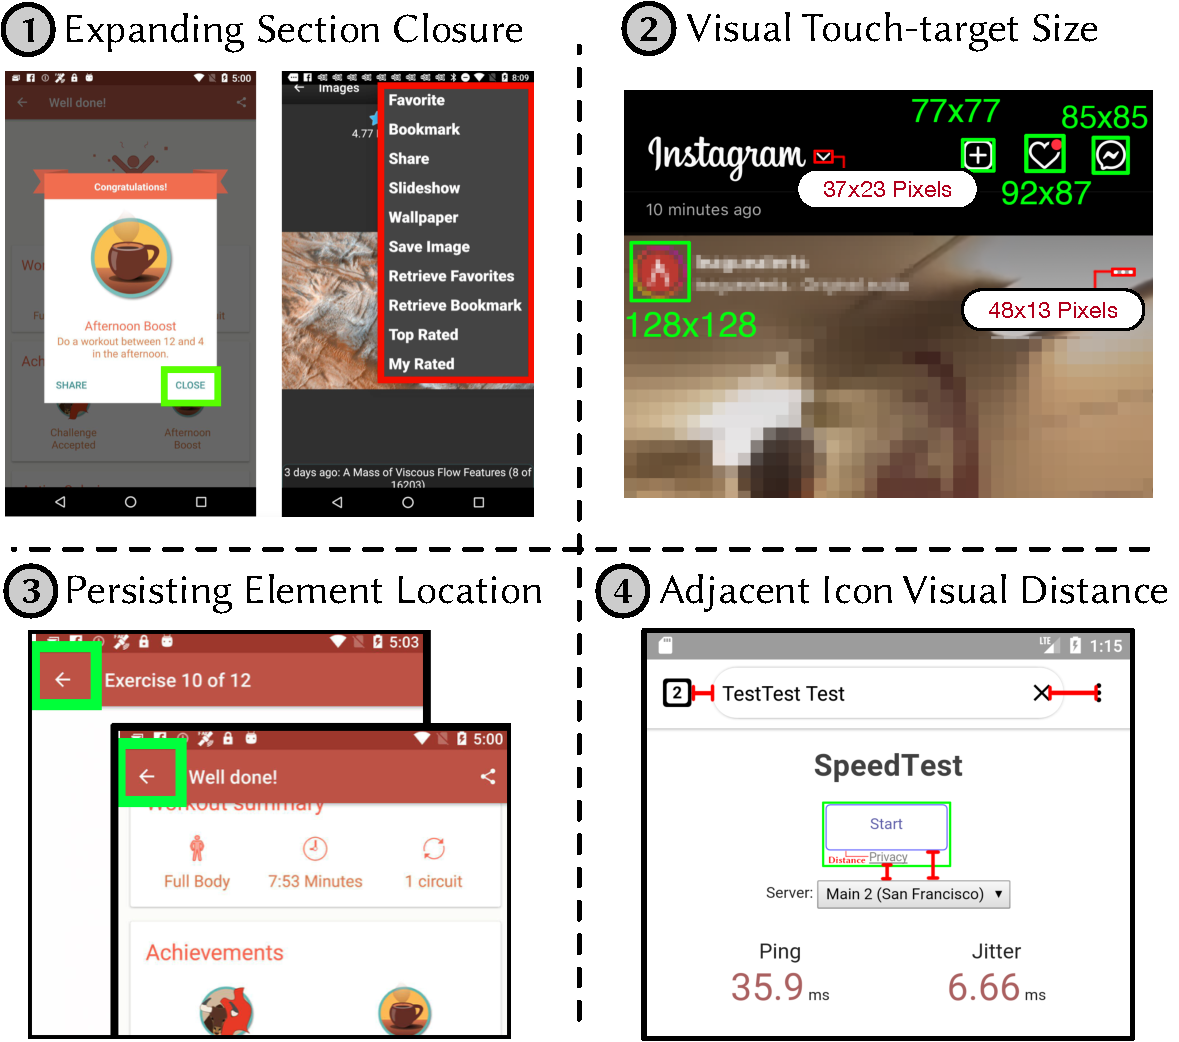
\includegraphics[width=0.6\textwidth]{imgs/guidelines.pdf}
    \caption{Illustration of four studied accessibility guidelines}
    \label{AllDetectors}
\end{figure}


\subsubsection{Expanding Section Closure}
Pop up menus and modal dialogs can provide meaningful information to the user, but closing them can be non-trivial for motor-impaired users who utilize a switch, as they may not contain explicit UI elements for closing the menu or dialog. As such, UI design guideline advocated for by both Apple and Google~\cite{AppleAccess,GoogleAccess} state that such closure UI elements should be present and easily interactive. Many expanding sections can be closed through a swiping gesture to dismiss the section or an external tap on the screen not within the bounds of the expanding section. Both of these options pose an accessibility issue for motor-impaired users due to the need for gestures and assumptive tapping on non-intuitive screen locations. A violation and adherence to this guideline is illustrated in Figure~\ref{AllDetectors}-1. Detecting UIs that violate this design guideline can be difficult as it requires automatically identifying (i) whether a pop-up menu or modal dialog is present within a given screen, and (ii) whether or not a UI element supports closing the pop-up. 

\subsubsection{Visual Touch-Target Size}
Motor-impaired users who experience tremors in their hands can experience difficulty tapping precisely on icons. This makes it difficult for them to interact with elements as intended. Apple and Google suggest minimum UI element sizes of 44x44 pixels and 48x48 pixels respectively, such that users with minor motor impairments can more easily tap icons~\cite{AppleAccess,GoogleAccess}. 
Typically, the ``size'' of a UI element is defined by the \textit{touchable area} of that element, and not the \textit{visual area} occupied by the pixels of a given element. However, as stated above, it is important to provide sizable \textit{visual} touch targets to users with more limited motor control, such that they can better hone their more limited movements to tap desired UI elements. Most past work that aims to identify icons or UI elements that do not meet a given minimum threshold read UI metadata to examine the ``touchable area'' only, even if the visual size of the icon does not fill the entire area. Thus, this can create a disconnect between the \textit{visual} touch target size, and the \textit{touchable area}. An example of this is shown in Figure \ref{AllDetectors}-2. The 
\includegraphics[width=0.04\linewidth]{imgs/insta-icon.png} icon next to the Instagram logo has a touch target size of larger than 44x44, however, the visual size of this icon is quite small, a making it difficult to tap. Detecting such issues can be difficult as it requires automatically inferring the visual area on a screen occupied by a given UI element. \MotorEase aims to overcome this issue by leveraging optical character recognition and neural object detection techniques.

 of just motor-impaired users. 
\vspace{-0.5em}
\subsubsection{Persistent Element Location}

Applications link various screens together to aid users in completing complex tasks, however, certain UI elements need to exhibit \textit{consistent} placement to assist switch users with anticipating UI element scanning. This guideline specifies that icons that appear across multiple screens should appear in the same general area of the screen~\cite{AppleAccess,GoogleAccess}. This means the locations of elements such as back buttons or search icons that appear across multiple different screens should remain consistent. An example of a back button with a consistent location is illustrated in Figure~\ref{AllDetectors}-3. Violations of this guideline can be difficult to detect as it requires automatic identification of corresponding UI elements across screens which may exhibit visual variability (e.g., displayed on different backgrounds).


\subsubsection{Adjacent Visual Icon Distance}

The design and placement of interactive icons that signal functional affordances is critical to ensuring a positive user experience, particularly for individuals with motor impairments. For users who may struggle with fine motor movement, it can be difficult to tap a single location on the screen without accidental triggers of other areas~\cite{Kong21}. As such, the \textit{Adjacent Visual Icon Distance} guideline states that adjacent ``clickable'' UI elements should be positioned at least eight pixels apart from one another.  This can be challenging as it again requires the automated inference of the visual area occupied by different UI elements. In this context, the issue of miss-clicks may trigger unwanted functions within the app. It is imperative that interactive icons can be accessed individually without any risk of accidental activation of adjacent icons. Google's Android Accessibility Guidelines \cite{GoogleAccess} stipulate that icons must be placed a minimum of 8 pixels apart to prevent miss-clicks by users with tremors or other motor impairments. Ensuring proper icon placement is crucial in enabling users with fine motor difficulties to interact with these icons effectively and without any possibility of error. Thus, the significance of this detector lies in the need to test for proper distance between icons.
An example of this is shown in Figure~\ref{AllDetectors}-4, wherein the ``Start'' and ``Privacy'' elements are located too close to one another and may result in accidental, unintentional triggering of the components by a motor-impaired user.

\subsection{\MotorEase Approach}


\begin{figure}[t]
	\centering
    \includegraphics[width=0.55\textwidth]{imgs/MotorEaseOverview.pdf}
    \caption{Overview of \MotorEase's Workflow}
    \label{fig:overview}
\end{figure}

\MotorEase is an automated approach that aims to detect motor-impairment accessibility guideline violations by analyzing UI metadata and screenshots collected via automated input generation (AIG) tools (i.e., automated app crawlers, UI testing tools). MotorEase operates in three stages, and implements four guideline violation detectors, as depicted in Figure ~\ref{fig:overview}. First, an AIG tool is run on a target application to produce a set of screenshot and uiautomator XML files (i.e. UI metadata) before and after each AIG tool action. We tailor our approach to utilize UI metadata generated using the uiautomator framework, which captures UI layout information in a structured XML format, as this is most prevalent utility used by recent Android AIG tools~\cite{mao2016sapienz,li2017droidbot,Gu:ICSE'19,Moran:ICST'16,crashscope,Su:FSE'17,Linares:MSR15,Linares:ICSME'17,Linares:ICSME'17-2,Zhao:FSE22}. It should be noted that \MotorEase does not require any pre-existing test cases, but instead can be used in conjunction with any of the AIG tools listed above. Second, \MotorEase utilizes a series of four \textit{violation detectors} to analyze the screenshots and UI metadata to determine if the target application failed to follow motor-impairment guidelines. Finally, \MotorEase collects the information from the detectors and compiles an \textit{accessibility report} that informs developers of accessibility guideline violations.



\subsubsection{Detectors}

The core components of \MotorEase are its four accessibility guideline violation detectors. Detectors \circled{1}, \circled{2} and \circled{4} operate upon \textit{single} uiautomator XML files, screenshots, in the form of PNGs, or both. Detector \circled{3} takes as input a series of \textit{multiple} \texttt{\small XML} and screenshot pairs. In the remainder of this section, we describe the technical underpinnings of each of \MotorEase's detectors.

\subsubsubsec{\textbf{Expanding Section Closure Detector}}

%\begin{figure}[h]
%    \centering
%    \includegraphics[width=0.45\textwidth]{imgs/expanding1.jpg}
%    \caption{Classification of Closing Expanding Sections}
%    \label{expandingClass}
%\end{figure}


The expanding sections detector aims to identify pop up messages or slide-in views that lack a visible means to close the section. Objects or text that imply closing the section is what \MotorEase aims to detect, if it cannot detect these, then a given screen with a dialog box or section is considered to be in violation of the guideline. 
This detector begins by determining whether the screen has an expanding section and then extracting it from the screenshot. This is done by identifying the largest element on the screen. \MotorEase extracts the largest \emph{android.widget.FrameLayout} and the largest \emph{android.widget.ListView} on the screen whose size is not the entire screen as the pop up screen or the slide-in list menu. %As a result, we built a tool that extracted all of the pop outs in a screen. 
An example of this is shown in Figure \ref{extractedSec}.

\begin{table}[h]
%\vspace{-1em}
\centering
\small
\renewcommand{\arraystretch}{2}
\caption{Mapping of Sample Lexical Patterns to detect Closure}

\label{tab:text-patterns}
\begin{tabular}{p{15cm}}
\hline
\textbf{Initial Closure Words}\\

"close", "cancel", "dismiss", "done", "ok", "finish", "return"\\
\hline
\textbf{GLoVE Embedding Words}\\

 "deny", "allow", "exit", "end", "terminate", "quit", "back", "stop", "ignore",  "proceed", "save","apply", "submit", "confirm", "abort", "decline", "reject", "ignore"\\
\hline
\end{tabular}
\end{table}

Once \MotorEase has extracted each of the expanding sections, it then aims to determine whether the pop-up or section provides a clear means of closing it. In order to offer a robust solution, \MotorEase accomplishes this via two main procedures: (i) Semantic Text Matching and (ii) Icon Detection. This is due to the fact that closure controls can have either textual (i.e. the word ``exit'') or visual (i.e. an $\times$ icon) signifiers that indicate functionality.

\noindent\emph{\underline{Semantic Text Matching:}} \MotorEase's semantic matching technique defines a certain set of keywords that are likely to signify an element that can close an expanding section or pop-up.  
These keywords comprise common lexical patterns derived through two authors of the paper examining expanding sections that appear in 1500 randomly sampled screenshots from the RICO dataset~\cite{Deka:UIST'17}. The RICO dataset, comprising 9,000+ Android apps and 66,000+ screenshots, serves as a popular resource for mobile app research given its diverse set of screens and apps. We randomly sampled 1500 screens as it represents a statistically significant sample size of the ~66k screenshots present in the RICO dataset (95\% confidence level and 2.5\% margin of error). These words were terms that implied a closure or completion action, i.e. ``close'', ``dismiss'', ``cancel'', ``ok''. To ensure that the selected words for semantic matching were relevant, we employed a manual process in which two authors reviewed the randomly sampled dataset for expanding elements and words that implied closure. The resulting set of words was agreed upon by the authors as suitable for the task. To further expand this set of words, we further utilized GloVe embeddings~\cite{glove} to compare the original selected words to the entire dataset. Glove embeddings capture semantic relationships between words by considering global word co-occurrence patterns, resulting in dense vector representations that preserve meaningful similarities between words~\cite{glove}. We extracted additional words that exhibited a cosine similarity of at least 0.95 to the GloVe embeddings of the original selected words. This approach enabled us to carefully curate a comprehensive set of words for semantic matching that accurately represented closure. We provide the complete list of 25 closure words in Table~\ref{tab:text-patterns} -- as our experiments illustrate, we found these words to generalize well to our experimental benchmark. %We then moved onto extracting the text from each of the sections. 

\begin{figure}[h]
    \centering
    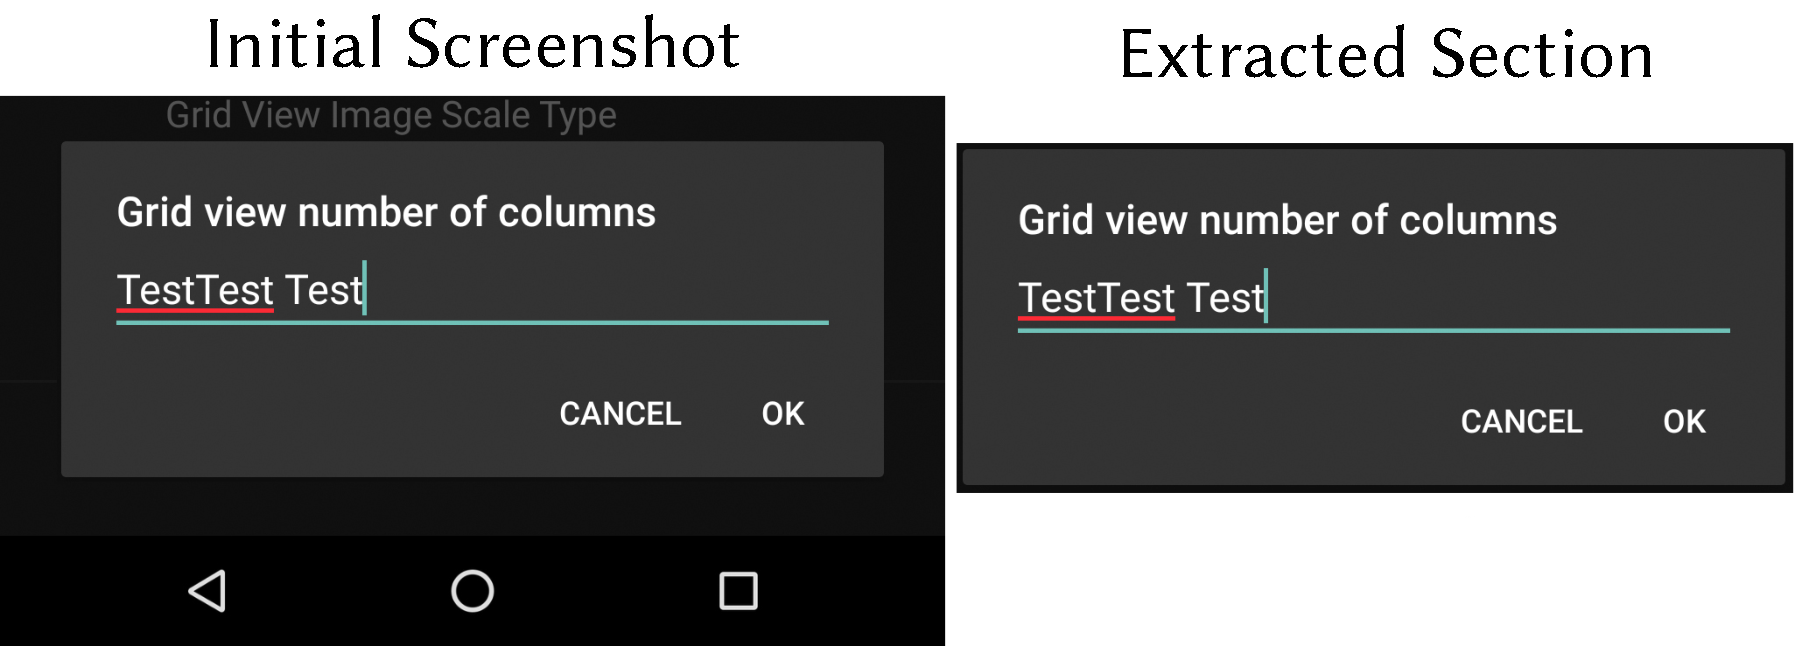
\includegraphics[width=0.7\textwidth]{imgs/extracted-section.pdf}
    \caption{Extracted Expanding Sections}
    \label{extractedSec}
\end{figure}

To extract the text from each image, \MotorEase leverages a combination of Google's Optical Character Recognition (OCR) text extraction~\cite{ocr}, which is based on the EAST OCR technique~\cite{zhou2017east} and the text present in the \texttt{\small uiautomator} \texttt{\small XML} file. We use both methods of text extraction as text displayed on the screen via images is often not captured in the \texttt{\small uiautomator} \texttt{\small XML} files. This method provides a binary classification for the presence of text that indicates a means to close the pop-up. If there are no matching extracted terms, \MotorEase then proceeds with icon detection.


\noindent\emph{\underline{Icon Detection:}} Icon detection is used to identify specific closing icons, i.e. $\times$, hamburger icon, checkmark, etc. Two authors examined the same set of 1500 screens from the RICO dataset discussed above and compiled a set of base icon types to train an image detection model in order to detect these icons. The chosen base icons are shown in Figure~\ref{fig:icons}. To accurately perform this detection, we trained a neural object detection model on a diverse set of examples of these identified icons, through a process we describe in detail below. 

\begin{figure}[t]
    \centering
    
\includegraphics[width=0.7\textwidth]{imgs/closure-icons.pdf}
    \caption{Base Closure Icons}
    \label{fig:icons}
\end{figure}

Training a neural object detection model typically requires a large-scale dataset with annotated examples of the target icons. To derive such a dataset, we \textit{automatically} constructed a realistic, synthetic dataset of icons that represent menu/pop-up closing. To do this, we extracted icon images with transparent backgrounds from the Fontawesome~\footnote{\url{https://fontawesome.com}} and Flaticon~\footnote{\url{https://www.flaticon.com}} image repositories until five icons for each icon type were identified that varied in color and style. Note that these icons do not directly appear in our evaluation dataset. We then superimposed these icons into random locations on screenshots derived from the RICO dataset~\cite{Deka:UIST'17}. During the analysis of the 1500 RICO screenshots two authors determined that a majority of icons on the screen were mathematically smaller than 10\% of the total screen size and larger than 2\% of the screen size. The screen size in question are the 1920x1080 pixel dimensions of the screen, limiting the maximum icon size to 192px and minimum icon size to 38px. Therefore, when an icon was superimposed on a screen, we varied their size between 2\% and 10\% of the screen area so that they remained relatively similar to the screens in the dataset. In this manner, we generated a dataset of 7,291 images (separate from the 1500 images sampled earlier) all with labeled and fully-localized icons on them (one per screen, spread evenly across the variations of our six icon types) and divided this into training and testing sets following an 80/20 split, 5,832 images for training, 1,458 for testing. We then used this dataset to train a Faster-RCNN object detection technique~\cite{ren2015faster} using the the torch-vision API~\cite{torchvision}. We generated $\approx$ 7k images as past work that uses a similar approach for icon detection was able to train an accurate model with this scale of data~\cite{Cardenas:ICSE'20,Cardenas:TSE23,Havranek:ICSE'21}. Our trained model was able to achieve over 95\% accuracy on the test portion of our dataset. 

%In our survey of the dataset, we noticed that these icons can be less than a tenth of the area of the entire screen, which means we needed a model that would precisely be able to only detect these icons on a large screen. In order to do that, we decided to overfit a multi-classification PyTorch image detection model \cite{torchvision}. 

%Overfitting a model to detect six specific icons requires an abundance of niche data that contains those exact icons. 

\MotorEase passes the cropped out expanding sections to the model in order to detect the icons. 
This detector works by first checking for semantic text matches and if there is no match, it then checks for icons. \MotorEase performs text pattern matching first because of the potential for X icons on the expanding section \textit{not} related to closing the icon. Had we done the icon detection first, the X icons to delete text in the text-fields would have been detected by the object detector. This means that this screen would have been classified as closable even though the X icons do not imply closing of the section. Therefore we use both the text and images on the expanding sections to try and classify if it can be closed. 
If neither technique can pick up on a pattern or icon, \MotorEase reports the section as a violation to the expanding section guidelines, capturing the the screenshot name, FrameLayout/ListView name, and violation and make it known to the developer. %We do this by providing the screenshot name, FrameLayout/ListView name, and violation or non-violation.}
%Figure \ref{expandingGood} illustrates an example of why the detector is constructed in this way. This screen is an example of a closable expanding section because of the explicit cancel button at the bottom left. The pattern matching is able to detect this and classify this screen as collapsible. 
%The reason \MotorEase performs the pattern matching first is due to that  of the other X icons on the screen. Had we done the icon detection first, the X icons to delete text in the text-fields would have been detected by the object detector. This means that this screen would have been classified as closable even though the X icons do not imply closing of the section. Therefore we use both the text and images on the expanding sections to try and classify if it can be closed. 
%\begin{figure}[h]
%    \centering
%    \includegraphics[width=0.36\textwidth]{imgs/goodExpanding.jpg}
%    \caption{Expanding Section Closure Detection}
%    \label{expandingGood}
%\end{figure}


\subsubsubsec{\textbf{Visual Touch-Target Detector}}

%The touch-target detector takes a deeper look into interactive icons on the UI. 
This detector uses both the screenshot and its corresponding XML file. It starts by processing the XML file and extracting the bounds for all elements which are clickable. XML has various properties in its metadata to describe an element, and if an element has a \emph{"True"} in the \emph{"clickable"} field, we determined that it is meant to be clicked on  or interacted with. 
This detector aims to identify elements that have a visible area that is smaller than their tappable/clickable bounding box. Hence with this detector, \MotorEase aims identify elements whose \textit{visual} size are under 48x48 pixels~\cite{ANDRDesign}, even when the reported touchable area (as indicated by \texttt{\small uiautomator}) may be larger than 48x48. The bounding boxes in \texttt{\small uiautomator XML} files can show a bounding box whose size is larger than the actual size of the icon. 
An example of this is shown in Figure~\ref{boundBox}. The true bounds of an icon corresponds to the visible area occupied by the icon. This can make these bounding boxes appear to be guideline abiding since they are generally larger than the true, visible bounds of the icon they hold. 
In order to identify these cases, \MotorEase adds 15 pixels to the width and height of the bounding boxes of each clickable item to extract the entire icon, before cropping the enlarged icon from the image. %This is done to extract the entire bounding box and icon in the image. %, as, bounding boxes can be accurate to their true size, so we want to ensure that we are able to extract the entire element from the screen. 

%\KEVIN{This is image is too large, images should be appropriately sized.}

%\begin{figure}[t]
%    \centering
%\vspace{-2em}
%    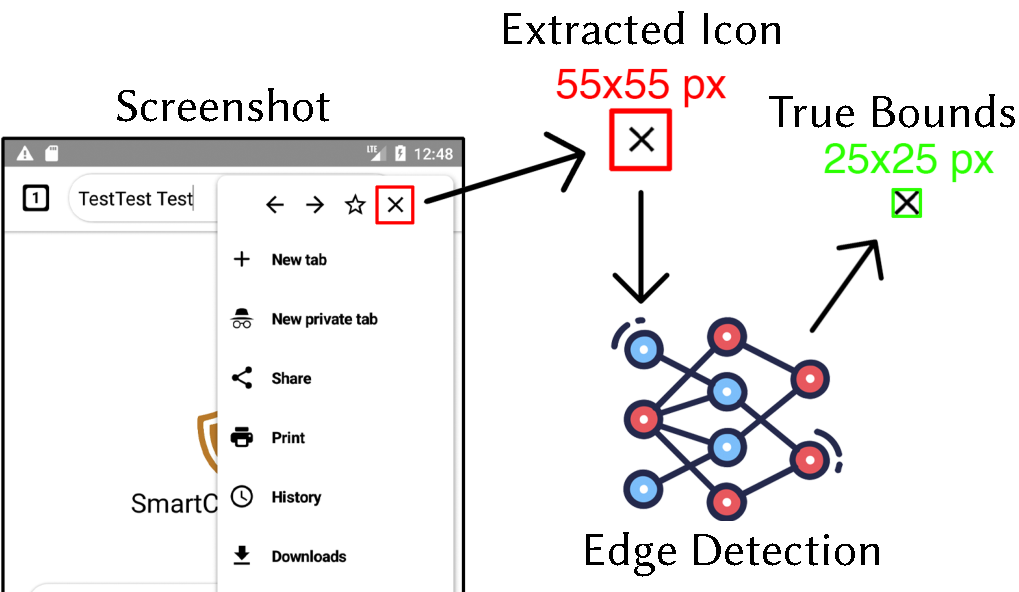
\includegraphics[width=0.45\textwidth]{imgs/extracted-icons.pdf}
%    \caption{Touch-Target Violation Detection Process}
%    \label{touchViolation}
%\end{figure}

\begin{figure}[t]
    \centering

    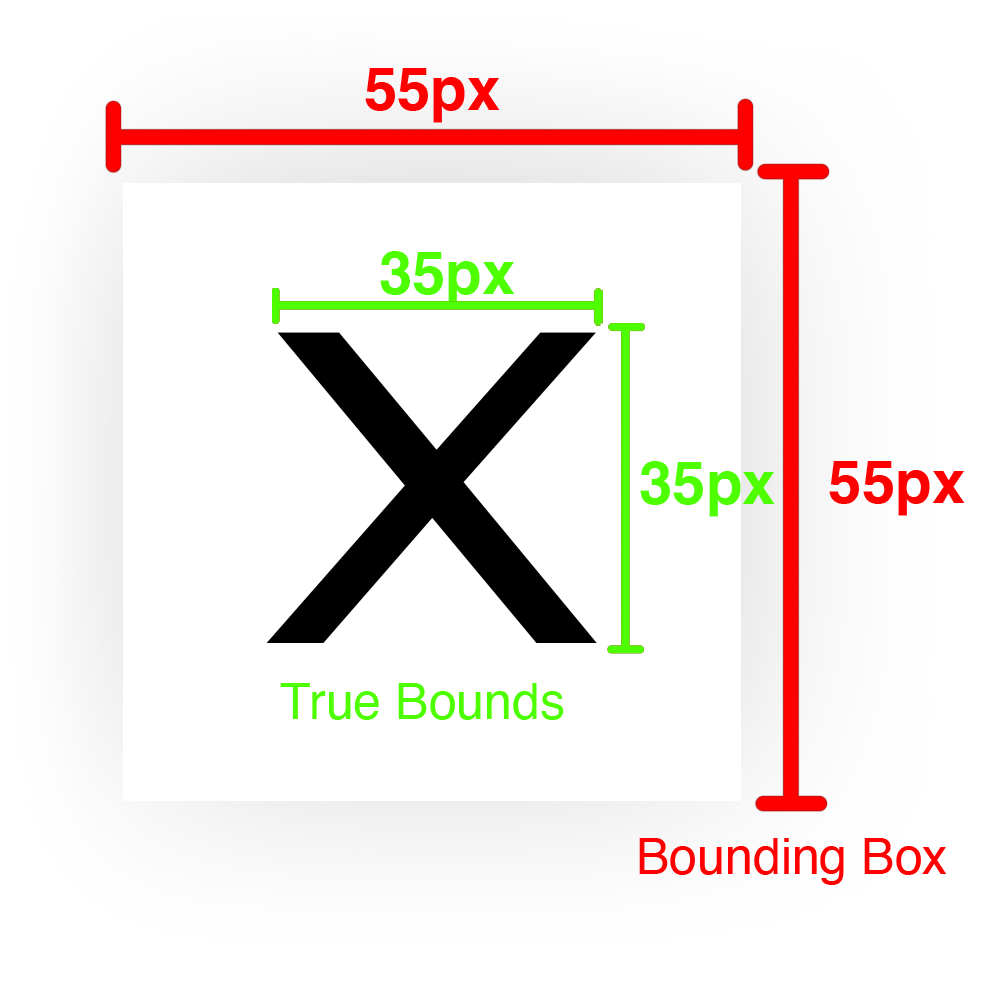
\includegraphics[width=0.35\textwidth]{imgs/boundBox.png}

    \caption{Example of Bounding Box vs. True Bounds}
    \label{boundBox}
\end{figure}

After \MotorEase extracts the element, it is used as input to an edge detection algorithm, implemented in the UIED tool~\cite{UIED}, which is an approach that combines both neural object detection and unsupervised edge detection to effectively segment mobile app UI screens. This edge detection procedure is able to derive the \textit{visual} bounds of a given UI element, and would identify the 35x35px edges for the "X" as shown in Figure~\ref{boundBox}. This procedure is applied to clickable icons extracted on each screen. Once the true edges are identified, \MotorEase is then able to then able to compare these bounds to the reported element size in the \texttt{\small uiautomator XML} file. If it is determined that the true element width or height is less than 48 pixels, \MotorEase labels that individual icon as a violation.  
\subsubsubsec{\textbf{Persisting Elements Detector}}
The persisting elements detector aims to identify an icon on a screen whose functionality remains the same, but location changes across multiple screens. An example of this is the navigation bar at the bottom of most applications. We expect that if the navigation bar is at the bottom of the screen on one screen, if a second screen has a navigation bar it should also be at the bottom of the new screen. 
This detector requires the use of both screenshots and \texttt{\small uiautoamtor XML} files from multiple screens, as \MotorEase directly analyzes properties of UI elements in the \texttt{\small uiautoamtor XML} files and compares the visual UI element similarity across multiple files.

\begin{figure}[t]
    \centering
    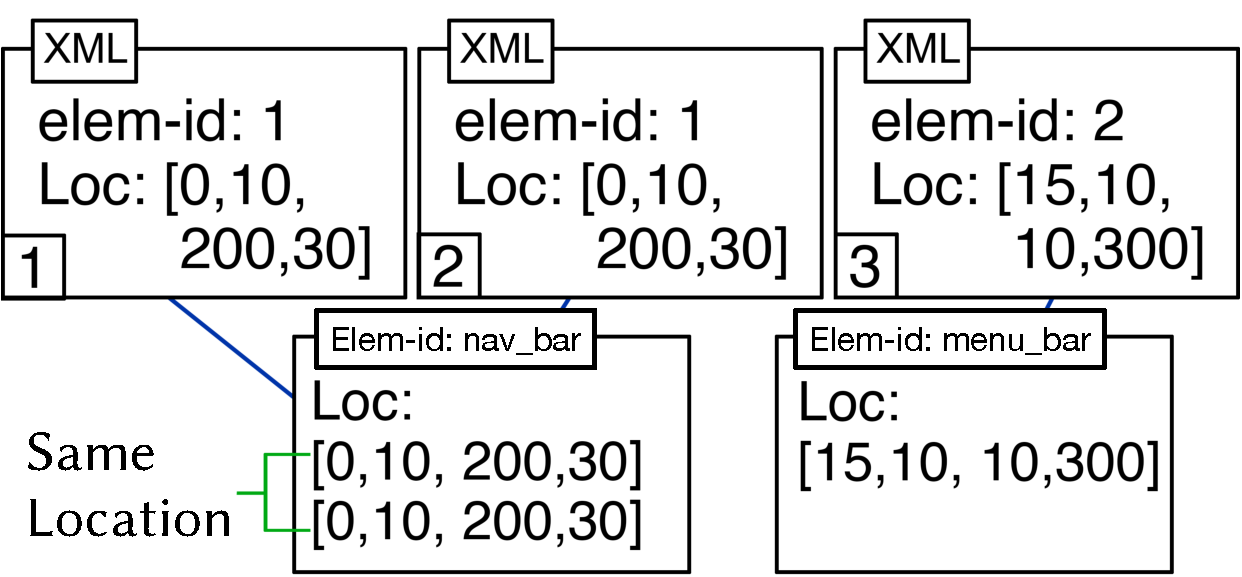
\includegraphics[width=0.6\textwidth]{imgs/persisting.pdf}
    \caption{Detection of Persisting Elements}
    \label{persistingDetect}
\end{figure}

%We looked at the dataset and found that dynamically produced XML files provide element identifications(IDs) for each element on the screen. We were able to leverage the IDs for each element across each screen to see if their location changed. 
This detector parses all of the \texttt{\small XML} files for a given application and records all of the UI element IDs. Then, it collects the location(s) across all \texttt{\small XML} files for each individual element ID. If there was more than 1 instance of a given ID across multiple screens, \MotorEase checks to determine whether the location bounds were the same as well as checking if the elements within those bounds are visually similar (95\% similar according to pixel-based mean squared error). If they are not, it deems it a violation of the persisting element guideline. This ensures that \MotorEase is checking every element in the application while checking to see if the icons with similar IDs have similar visual properties.  
If there is an element that appears across the \texttt{\small XML} files more than once, \MotorEase examines them to see if the location is the same for the element. 
It relays this information back to the developer by providing the ID of the violating element in the generated Accessibility report. 
\subsubsubsec{\textbf{Visual Icon Distance Detector}}


The icon distance detector is designed to analyze icons on a screen and determine whether the visual distance between any two icons is less than 8 pixels, which combines findings from Kong et al. ~\cite{Kong21} regarding visual icon size/spacing and recommendations from Google's accessibility Guidelines~\cite{GoogleAccess}. T

\begin{figure}[h]
    \centering
	
    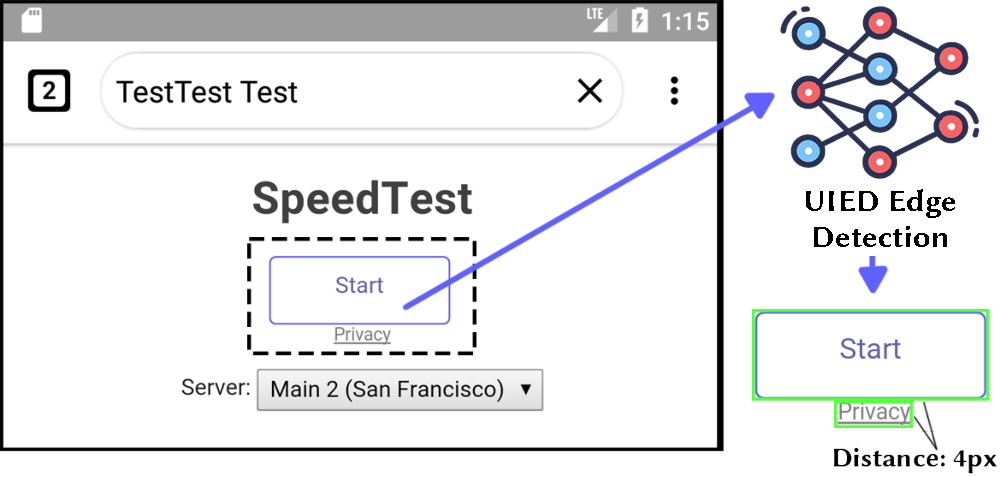
\includegraphics[width=0.5\textwidth]{imgs/visual-distance.pdf}
    \caption{Visual Icon Distance Detection Process}
    \label{iconViolation}
\end{figure}

his detector analyzes a XML and screenshot pair, and extracts all of the \emph{clickable} elements on the screen using the \texttt{\small uiautomator} metadata. Once the clickable elements are identified, \MotorEase crops out the icons and sends them as input to UIED~\cite{UIED} to find the true visual bounds of the icon via edge detection. The true bounds are then used to subtract the padding from the initial touch target to the visual touch target. These modified bounding box values are then stored, and the detector iterates through all of the other icons on the screen to calculate the distance between the target UI elements and all other elements. The distance between the bounding boxes is calculated by determining the horizontal, vertical, or diagonal distance in pixels between two bounding boxes on a screen.Once the distance between the icons is computed, \MotorEase checks whether there is a distance is less than 8 pixels. If a violation is detected, \MotorEase includes a description of the UI elements in the generated accessibility report allowing the developer to address the issue and improve the accessibility of their application.

\subsubsection{Accessibility Report Generation}

The accessibility report is generated using the target app screenshots that contain violations and a generated markdown file, with filenames to specific images of violations for each detector. We developed textual templates for each type of violation that are used by the report generation engine to automatically describe the accessibility violations by filling in the templates with information the \MotorEase analysis. This accessibility report aims to provide a comprehensive account of accessibility issues within a given app so that developers are able to take this information to make any changes they may need in order to make their apps more accessible.


\subsection{Evaluation Methodology}


\newlist{questions}{enumerate}{2}
\setlist[questions,1]{label=RQ\arabic*.,ref=RQ\arabic*}
\setlist[questions,2]{label=(\alph*),ref=\thequestionsi(\alph*)}

%RESULTS

%- how well did \MotorEase perform on the datasets

%- how well does each single detector perform



%EVALUATION

% combine all the tables for the dataset 
% add the research questions in the design of the eval design 
% explain how we measure the efficacy of each research question  

%- how we plan to do the experiments

%- how the data was labeled 

%- how did we create different datasets for each detector 

%- what the detectors output and how we plan to ma\\MotorEasetch that to the data

In this section, we describe the procedure we used to evaluate \MotorEase. The goal of our empirical study is to assess the accuracy, and practical utility of the approach. The main \textit{quality focus} of our study is to determine the extent to which \MotorEase is able to detect accessibility violations in applications.
To achieve our study goals, we formulated the following five research questions: 
\begin{itemize}
		\item{\textbf{RQ$_1$} \textit{How accurate is the Expanding Section detector?}}
		\item{\textbf{RQ$_2$} \textit{How accurate is the Visual Touch Target detector?}}
        \item{\textbf{RQ$_3$} \textit{How accurate is the Persisting Element detector?}}
        \item{\textbf{RQ$_4$} \textit{How accurate is the UI Element Distance detector?}}
		\item{\textbf{RQ$_5$} \textit{Does \MotorEase identify a limited number of false positive and negative violations?}}
\end{itemize}
        
\subsubsection{RQ$_1$ - RQ$_4$: Violation Detection Capability}
 
\MotorEase is one of the first tools to support the detection of violations of accessibility design guidelines targeting motor-impaired users, and accomplishes this via understanding the visual and textual modalities Android UI screens. 
Given that prior techniques are not able to explicitly detect the design violations that \MotorEase targets, by using the visual comprehension of the screen, we both derived an entirely novel benchmark and designed an evaluation methodology that tests each of its four detectors individually to determine their accuracy, precision, and recall. In addition, we also examine the false positive and false negative rates to better understand the practical utility of \MotorEase. The evaluation metrics used in this study provide insights into the ability of each detector to identify true positives and true negatives. Accuracy gives us an overall ability to deduce each detectors ability to detect true positive (TP) and true negative (TN) values accurately. Note that we balance the positive and negative samples in the \MotorCheck benchmark to allow for an informative accuracy measurement.
	
	\begin{center}$Accuracy = \frac{TP+TN}{TP+TN+FP+FN}$\end{center}
	
\noindent In the context of our study, a True Positive ($TP$) is defined as the detection of an existing design guideline violation as defined in our ground-truth dataset. A false positive ($FP$) is defined as the detection of a violation when one does not exist. A False Negative ($FN$) occurs when our approach does not report a violation, but one exists in the ground truth. Finally, a True Negative ($TN$) occurs when the approach does not report a violation and one does not exist. In addition to accuracy, we also measure the precision and recall (as defined below) to provide a more complete picture of \MotorEase's performance. The results of \MotorEase were manually validated (i.e. two authors compared MotorEase's output to the ground truth.)
	
	\begin{center}$Precision = \frac{TP}{TP+FP}$ \hspace{1em}$Recall = \frac{TP}{TP+FN}$\end{center}

		
\noindent Given these two evaluation metrics, we can determine how accurately each detector works. \MotorEase's overall effectiveness can be derived by averaging the the accuracy/precision/recall across all four detectors, providing a comprehensive understanding of \MotorEase's ability to detect accessibility guideline violations. 


\subsubsection{RQ$_5$: M{\normalsize OTOR}E{\normalsize ASE}'s Practical Utility}

In order to investigate \MotorEase's practical utility, we also report both the false positive and false negative rate, as these reflect the need for a developer to sift through incorrect violation reports, or lost quality in terms of miss unreported violations. This helps to provide a more holistic picture of \MotorEase's performance.

	\begin{center}$False Positive Rate = \frac{FP}{FP+TN}$ \hspace{1em}$False Negative Rate = \frac{TN}{FP+TN}$\end{center}

\begin{table}[t]
	
	\begin{center}
	\caption{Expending Sections Detector Test Dataset}
	\begin{tabular}{ c|c|c|c } 
		\hline
		\textbf{Total Files} & \textbf{Close: Icon} & \textbf{Close: Text} & \textbf{Cannot Close} \\
		\hline
		483 & 27 & 214 & 242\\ 
		\hline
	\end{tabular}
	\label{t2}
	\end{center}
\end{table}

\begin{table}[t]
	\begin{center}

	\caption{Visual Touch-target, Persisting Elements, and Visual Icon Distance Test Datasets}
	\begin{tabular}{ c|p{.6in}|p{.53in}|p{.5in} } 
		\hline
		\textbf{Detector} & \textbf{Total Files/Apps} & \textbf{Violations} & \textbf{Non-Violations} \\
		\hline
		Touch-Target & 400 files & 176 & 224 \\
		\hline
		Persisting Elements & 49 apps & 24 & 25 \\
		\hline
		Icon Distance & 400 files & 42 & 358 \\
		\hline
		
	\end{tabular}
	\label{t1}
	\end{center}
\end{table}


\subsubsection{Derivation of the M{\normalsize OTOR}C{\normalsize HECK} Benchmark}
\label{subsec:dataset}

Given that no prior approach has targeted the motor-impairment design violations targeted by \MotorEase, we develop a novel benchmark called \MotorCheck which we discuss below. It should be noted that all of the accessibility violations of this benchmark are real, no synthetic violations were injected in it's construction -- instead real violations were rigorously manually annotated.

To derive the initial set of screenshots and xml files for \MotorCheck we applied the {\sc CrashScope}~\cite{crashscope} automated testing tool to 70 popular Android apps that are cross-listed on both FDroid and Google Play. To do this, we gathered a list of apps from F-Droid~\cite{Fdroid} and considered only those apps that were cross-listed on Google Play~\cite{GooglePlayStore} and had at least 1000 downloads -- providing some confidence in the popularity of the chosen applications. We provide a full list of these applications with download statistics and links in our online appendicies~\cite{appendix,site,zenodo}. During this process, we used one of {\sc CrashScope}'s exploration strategies to extract 2,864 screenshot/\texttt{\small XML} pairs. Note that the goal of our study in assessing \MotorEase's capabilities is independent of the coverage provided by the underlying testing tool, although {\sc CrashScope} has been illustrated to be competitive with other tools~\cite{Moran:ICST'16}. It should be noted that the screen coverage of \MotorEase is dependent upon the Android AIG tool that the approach is paired with. Given recent advances in AIG tools~\cite{wang_vet_2021}, \MotorEase can integrate with these new tools and take advantage of the improved coverage. Next, we describe the dataset derivation process for each detector. Note, given that the data labeling process is quite objective for violations of our identified guidelines, for each dataset, we had one author manually label each instance, and another author verified the results. During this process, no instances of conflicts were noted, again due to the largely objective nature of the labeling procedure. We provide an overview of the \MotorCheck benchmark data in Tables~\ref{t2}~\&~\ref{t1}.

\subsubsubsec{Expanding Section Closure Detector Dataset} In order to detect expanding sections, this detector requires an input screenshot and its corresponding \texttt{\small XML} file. In order to evaluate the detector and remove any bias, one author labeled expanding sections without closure elements until all CrashScope files were exhausted, resulting in 241 screens. Of the 241 screens that had an expanding section, there were 121 screens were FrameLayouts and the remaining 120 were ListViews. Then, in order to balance the dataset, an additional 242 screenshots without violations were randomly selected to complete the dataset, for a total of 483 screens. The additional screens without violations consisted of expanding sections that could be closed. Table~\ref{t2} provides more information on how the dataset was split between violations and non-violation samples. Labeling was done manually using LabelStudio~\cite{LabelStudio}. For the screenshots without violations, icon types and closure word types were labeled. If neither the icon nor text clearly showed a means of closing the section, it was labeled as a violation. 

\begin{table*}[t]
    \caption{Overall Results for \MotorEase Detectors \& Baselines}

    \centering
    \begin{tabular}{ c|c|c|c|c } 
         \textbf{Approach} & \textbf{Precision} & \textbf{Recall} & \textbf{Accuracy} & \textbf{F1-Score}\\\hline
        \textbf{{\sc\textbf{MotorEase}} (Viz T.-Target)} & 1.0000 & 0.6648 & 0.8525 & 0.7986\\ 
		\textbf{G-Accessibility Scanner (T.-Target)} & 0.5556 & 0.5085 & 0.6025 & 0.5310 \\\hline 
        \textbf{{\sc\textbf{MotorEase}} (Exp. Sec)} & 0.9042 & 0.9205 & 0.9123 & 0.9129\\ 
		\textbf{Groundhog (Exp. Sec)} & 0.6849 & 0.8659 & 0.7207 & 0.7648 \\ \hline
        \textbf{{\sc\textbf{MotorEase}} (Pers. Elem)} & 0.8214 & 0.9583 & 0.8776 & 0.8846\\
        \textbf{{\sc\textbf{MotorEase}} (Icon Dist)} & 0.7119 & 1.0000 & 0.9575 & 0.8317\\\hline
        \textbf{{\sc\textbf{MotorEase}} (All Detectors)} & \textbf{0.8594} & \textbf{0.8859} & \textbf{0.8999} & \textbf{0.8570}\\
       
    \end{tabular}
    \label{results}
\end{table*}

\subsubsubsec{Visual Touch-Target and UI Element Distance Detector Dataset} The touch-target detector requires screenshot and XML pairs to determine if the screens had a touch-target violation (i.e. XML) and visual bounds differed. In order to evaluate the detector and remove any biases, we randomly chose 400 screenshots and XML pairs generated by CrashScope stratified across our 70 applications. This sample size was used as it represents a statistically significant sample of the total number of extracted CrashScope screens (99\% confidence interval). Table~\ref{t1} provides the dataset splits between violations and non-violation samples. Labeling for these screenshots was performed manually. One author analyzed each of the screenshots and set a bounding box on each of the interactive elements on the screen using Label Studio~\cite{LabelStudio}. If the size of the bounding box was less than 48 in width or height, it was labeled it as a violation, else it was labeled as a screen without violations. Additionally, the author checked the distance between all components on these screens and labeled any instances where UI elements were less than 8 pixels apart. This was done for all 400 images. 

\subsubsubsec{Persisting Elements Detector}

The persisting elements detector requires multiple app XMLs in order to detect violations. The CrashScope dataset \cite{crashscope} contains 70 applications and their screenshots. We filtered out apps that only contained screenshots of similar screens, resulting in 49 applications, 24 of which had persisting elements that violated our guideline, and 25 of which adhered to our guideline. One author labeled each app as having a violation or not having a violation. During the labeling, this author also specified which specific screenshot exhibited the violation.

\subsubsection{Comparison to Baseline Techniques}

While the Accessibility issues that \MotorEase targets have not been explicitly targeted by past tools, there are two tools which are capable of detecting a subset of the accessibility violations identified by MotorEase. These two baselines are  Groundhog~\cite{Salehnamadi:ASE'22} and Google Accessibility Scanner~\cite{GoogleScanner}. We ran these two tools on the same \MotorCheck benchmark used to evaluate \MotorEase to keep the comparison fair and consistent, and we report the same metrics for both \MotorEase and the baseline techniques. Upon careful analysis of these baselines, Google Accessibility Scanner and Groundhog are only capable of detecting Touch-target size violations and Expanding Sections violations, respectively.

The first baseline tool we compared \MotorEase to in our updated evaluation is Google's Accessibility Scanner~\cite{GoogleScanner}. This tool operates directly upon the dynamic representation of the GUI as reported by uiautomator, and checks to whether the bounds of screen elements fall below the 48x48 dp threshold. To apply this tool, we launched the each app included in the MotorEase dataset on an emulator of the same screen dimension (1920x1080) and Android version as the screens in the MotorCheck benchmark  and manually navigated to the screen in question, and triggered the Accessibility Scanner tool. One author then manually compared the output results from Accessibility Scanner to the ground-truth visual touch-target size violations defined in \MotorCheck. We then reported the Precision/Recall/Accuracy and F1 Score Metrics.

The second baseline tool that we compared \MotorEase to is the Groundhog Accessibility tool~\cite{Salehnamadi:ASE'22}. We worked directly with the authors of the Groundhog tool, who were quite helpful after some initial issues initializing the tool, in order to apply Groundhog to the \MotorCheck benchmark. Groundhog functions by first sending touch-based actions to a given Android app screen running on an emulator or real device, and then attempts to exercise the same actions using one of Google's accessibility services, such as Talkback. Given the manner in which Groundhog works, the only Accessibility issue in \MotorCheck that it was applicable to is the Expanding Section guideline violations. To apply Groundhog to detect Expanding Section violations in \MotorCheck we launched a target on an Android emulator configured to the 1920x1080 screen size and Android version of the MotorCheck screens, and then ran Groundhog on the screen with an expanding section. Groundhog then navigated the screen both with and without assistive services to determine whether it could close the expanding section, if there was a discrepancy, this was reported by Groundhog. Then one author manually checked the output of Groundhog to determine if it was able to detect an expanding section violated the \MotorCheck guideline and could not be closed by a tappable element. We then reported the metrics seen in Table~\ref{results}



\subsection{\MotorEase Evaluation Results}

\subsubsection{RQ$_1$: Expanding Section Detector Accuracy?}

The expanding section detector performed well across nearly all of our studied metrics, as indicated in Table~\ref{results}. With a precision of .9042, F1-Score of 0.9129, and an accuracy of 0.9123, this detector shows promising results that it is capable of identifying a section's ``collapsibility'' accurately. This indicates that, by using \MotorEase, developers will have an increased chance of identifying sections that were designed without a method of closure which may impede motor-impaired users. 

\begin{figure}[h]
    \centering
    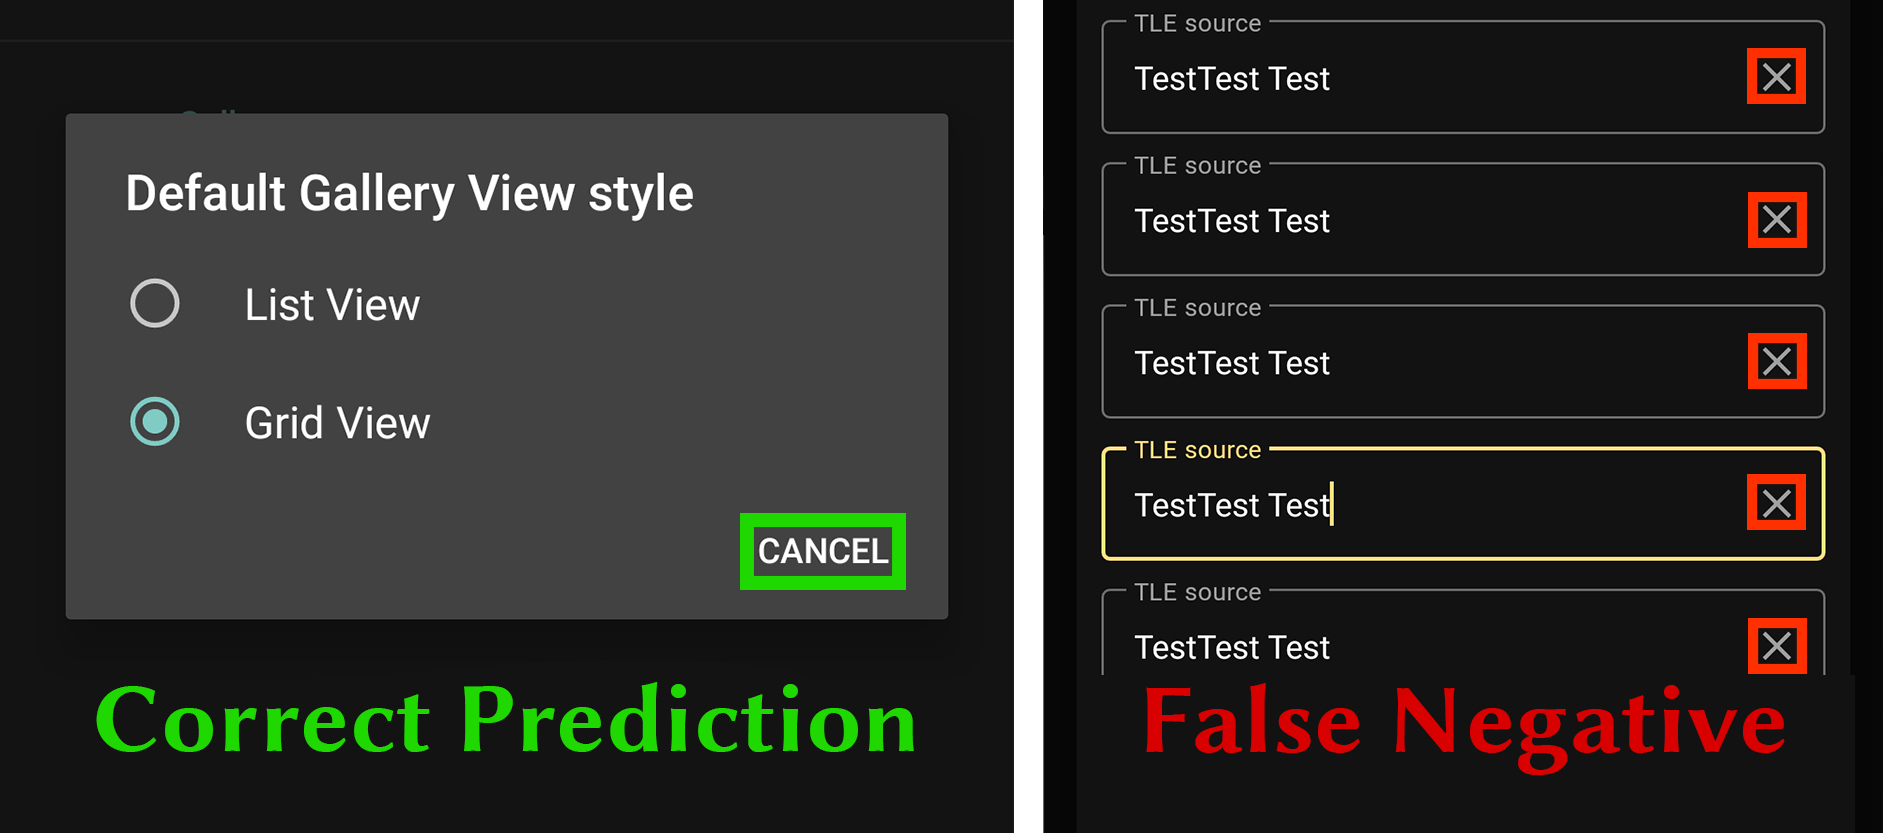
\includegraphics[width=0.5\textwidth]{imgs/expandingResultsV2.jpg}
    \caption{Expanding Section Closure Detection}
    \label{expandingResults}
\end{figure}

Importantly, as per Table~\ref{results} our approach surpassed the performance of Groundhog's ability to detect closable sections, with a precision of 0.6849, demonstrating its effectiveness in comparison. The difference between the two is attributable to the fact that \MotorEase and Groundhog do not have the same objective. MotorEase aims to detect the presence or absence of closing icons, while Groundhog aims to determine whether a closing icon can be accessed using an assistive service. If a closing icon is missing, Groundhog cannot detect it. Since there is no closing icon, Groundhog does not even attempt to close it using an assistive service. Groundhog relies on an accessibility service to detect icons on the screen, However, if the icon does not have any metadata indicating that it is an interactive, it is unable to interact with the icon and close it. \MotorEase's novelty lies in its ability to consider the visual presence of the icon independent of its metadata description. However, \MotorEase's detector does struggle to detect certain instances in the \MotorEase benchmark. An example of a successful and unsuccessful prediction is shown in Figure \ref{expandingResults}. The example on the left side is an expanding section that the detector correctly identified as collapsible. It is correctly identified by \MotorEase as a closing section because of the semantic matching's ability to generalize the word "cancel" as a means of closing the section. The image on the right is not collapsible but the detector deduced that it was collapsible. This was due to the use of X icons in the training data for the object detection model. The "X" icons used in this image imply the deletion of text, but this detectors object detection model is also trained to identify "X" icons that may be used to close the expanding section. It should be noted that this was an outlier in our dataset, and that the pattern for detecting "X" icons generally worked as expected.

\subsubsection{RQ$_2$: Visual Touch Target Detector Accuracy?}
 

The touch-target detector performed well as illustrated in Table \ref{results}. The detector exhibited perfect precision, an F1-Score of 0.7986, and an accuracy of 0.8525, showing encouraging results of its ability to detect and classify screens with touch target violations well.  Given the results, this detector is successfully able to give developers an insight into smaller icons that may inconvenience users with tremors and inaccurate touches. Importantly, our approach surpassed Google Accessibility Scanners's ability to detect visually small elements on the screen, which only had a precision of 0.5085, demonstrating its effectiveness in comparison. The primary reason for the gap in performance is that Google Accessibility Scanner is not able to check the \textit{visual} touch-target size, and can only parse the reported size from the \texttt{\small uiautomator} framework, which may not necessarily correspond to the visual touch target size. However, while nearly all violations returned by this detector are correct, it does tend miss certain types of violations. For instance, it cannot detect icons on the screen which are not labeled as clickable in the XML. By default, all elements on an android device have a clickable property with a boolean True/False label. If that property is labeled as False, \MotorEase does not consider the object to be clickable. Dynamically generated screenshots may not always have the metadata information for each element on the screen, and this absence of information was the main reason for incorrect or missed violations. This detector could be augmented in the future with work from the HCI community aimed at assessing icon tap-ability~\cite{Swearngin:CHI'19}. %This absence of information impacts the detector's ability to extract interactive elements on a screen since it cannot identify clickable elements, and this was the major reason for incorrect or missed violations.%Figure \ref{touchResults} shows an example of the touch target violations successfully detected by MotorEase's touch-target detector and ones it failed to detect. The three dot menus that were not detected were not labeled as clickable in the XML, therefore going undetected and never being sent to the edge detector to detect the true bounds.





\subsubsection{RQ$_3$: Persisting Element Detector Accuracy?}


This results of this detector are presented in Table \ref{results}. With a precision of 0.8214, F1-Score of 0.8846, and accuracy of 0.8786, this detector shows encouraging signs of viability. This detector's recall rate of 0.9583 suggests that the detector identifies true positives at a high rate. 

\begin{figure}[h]
    \centering
    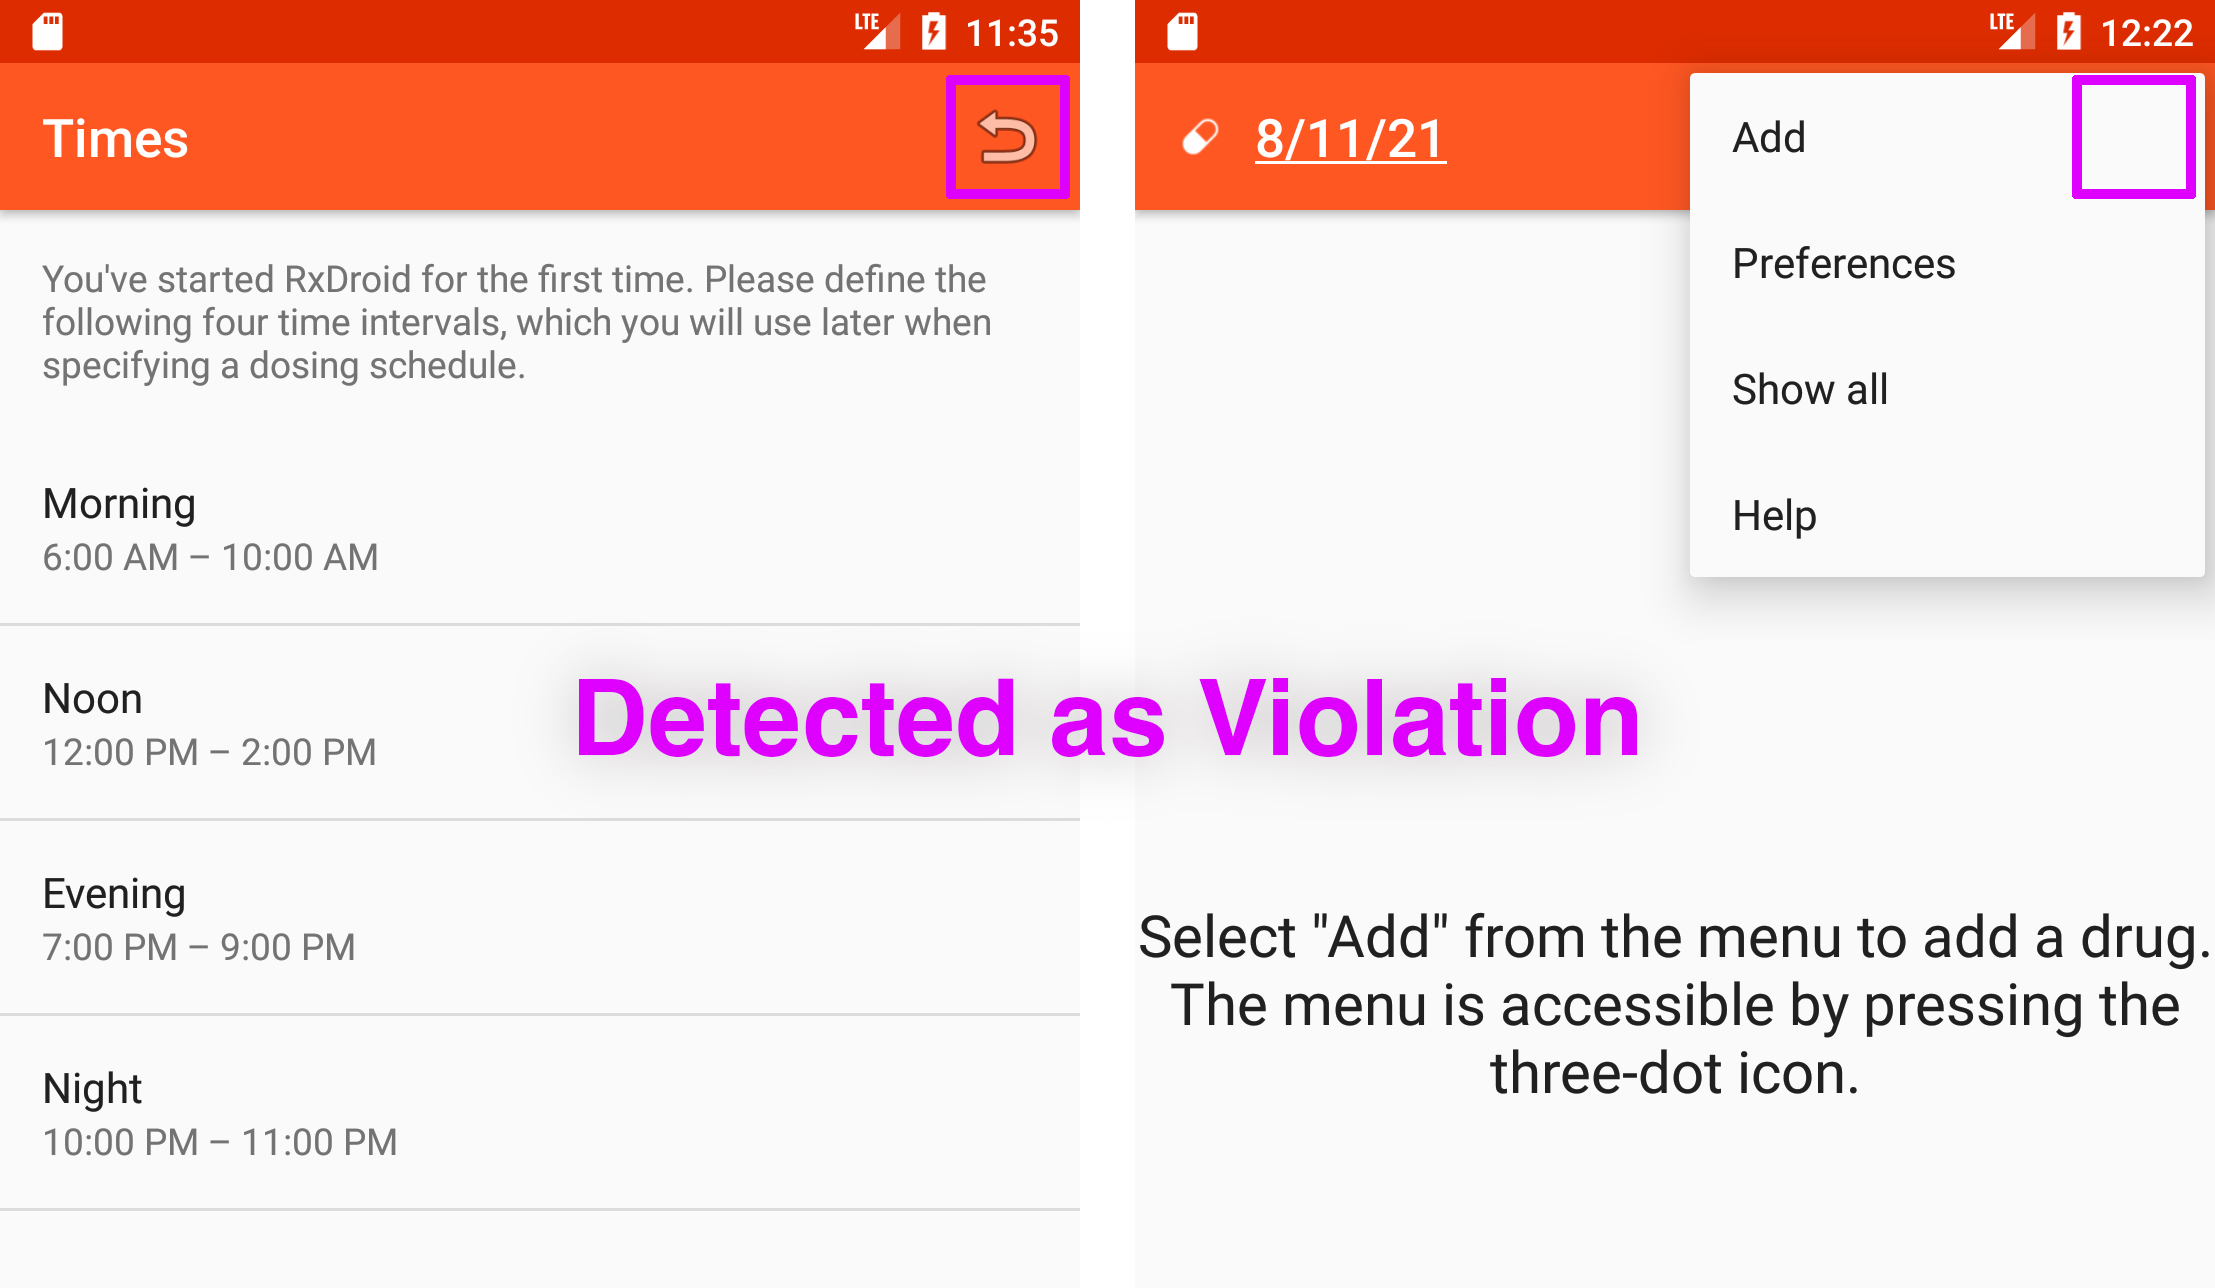
\includegraphics[width=0.5\textwidth]{imgs/persisstingResults.jpg}
    \caption{Persisting Elements Detection}
    \label{persistingResults}
\end{figure}

This detector, however, relies heavily on the XML to locate elements on the screen, which can lead to mis-classifications. One such example is shown in Figure \ref{persistingResults}. The example shows the undo icon on the screenshot on the left and a menu on the right side where the undo icon would be. The XML for this second screen has the undo icon in the data, but its bounds and information are missing since they are not visible on the screen. This was classified as a violation though it is not a violation. 


\subsubsection{RQ$_4$: Visual Icon Distance Detector Accuracy?}
This results of this detector are presented in Table \ref{results}. With a precision of 0.7119, F1-Score of 0.8317, and accuracy of 0.9575. This detector achieved a perfect recall rate, suggesting that this detector provides developers with a reliable tool that is capable of accurately detecting closely placed icons, prompting potential UI design and icon placement adjustments. 

\begin{figure}[h]
    \centering
    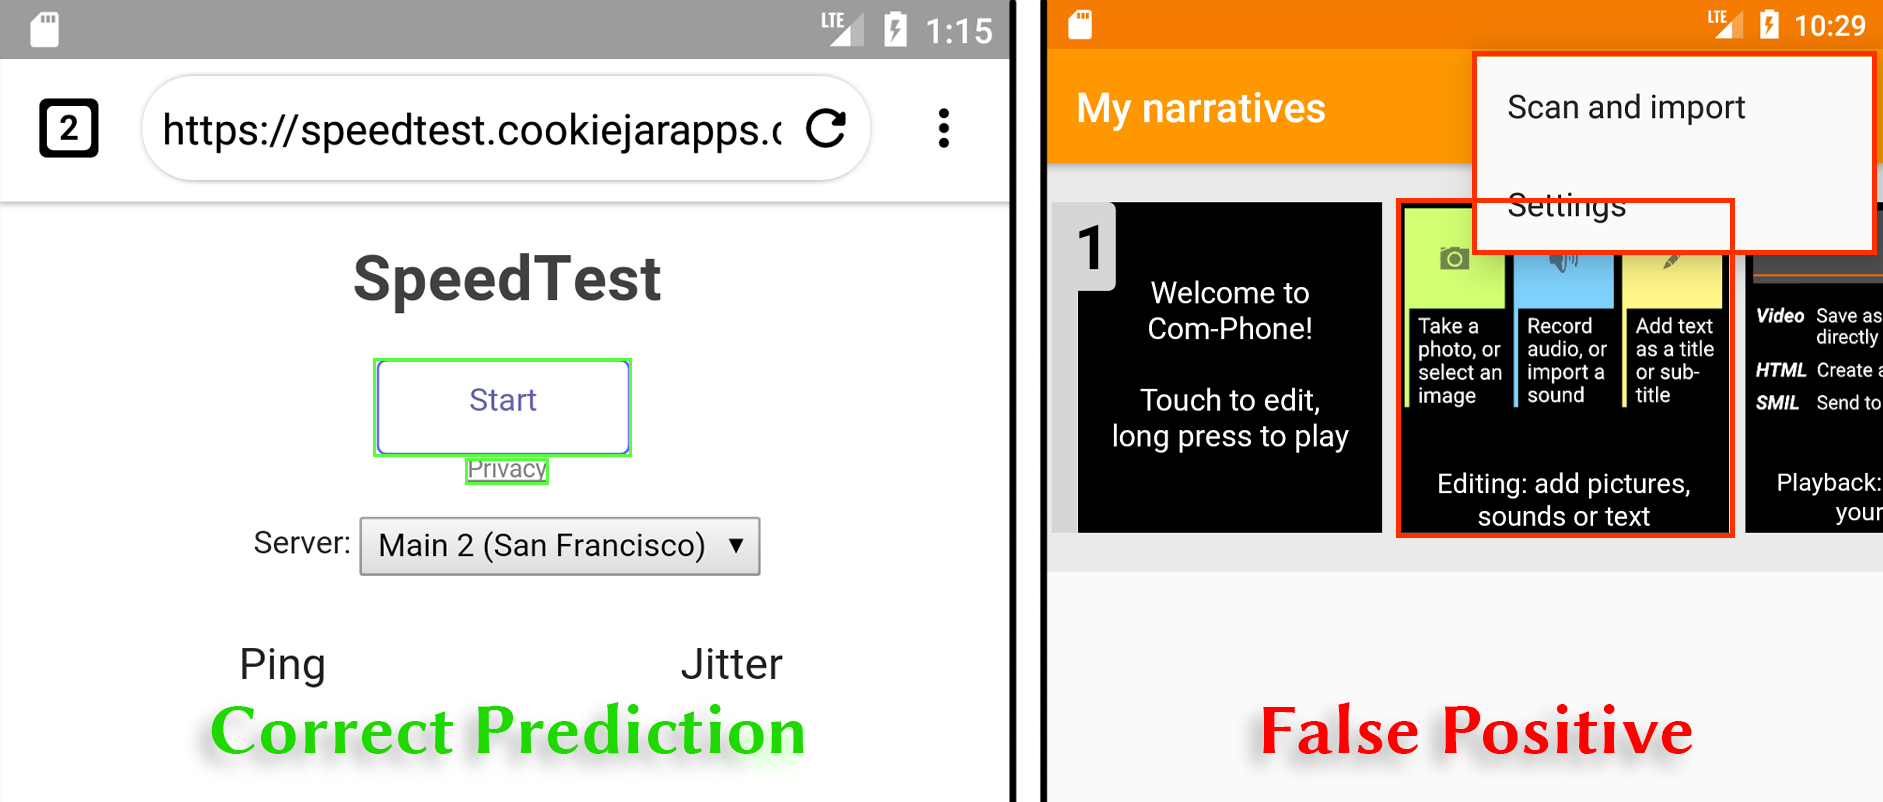
\includegraphics[width=0.55\textwidth]{imgs/IconDistanceResults.png}
    \caption{Visual Icon Distance Detection}
    \label{icondistanceResults}
\end{figure}

Like the Visual Touch-Target Violation detector, this detector relies heavily on the \texttt{\small uiautomator} metadata specifying clickable components, and the accuracy of the UIED element bound detector. The latter led to certain cases of inaccurate reporting of violations, due to incorrect overlapping bounds. Both of these examples are shown in Figure~\ref{icondistanceResults}. The first example shows a correct prediction where \MotorEase correctly identifies two icons on the screen and determines that they are not a minimum of 8 pixels in distance. However, Figure \ref{icondistanceResults} also has an example of a false positive prediction which shows an overlap of two elements on the screen. Due to the visual bounds of each overlapping, the distance between the two is 0, therefore predicting a false positive. 



\subsubsection{RQ$_5$: False Positives and Negatives}
The confusion matrices for the detectors are shown in Figure~\ref{matrices}, where green boxes illustrate predictions that matched the ground truth, and red boxes illustrate predictions that did not match the ground-truth. These figures provide 
	a visual representation of false positive and negative rates. 
	
	\begin{figure}[h]
    \centering
    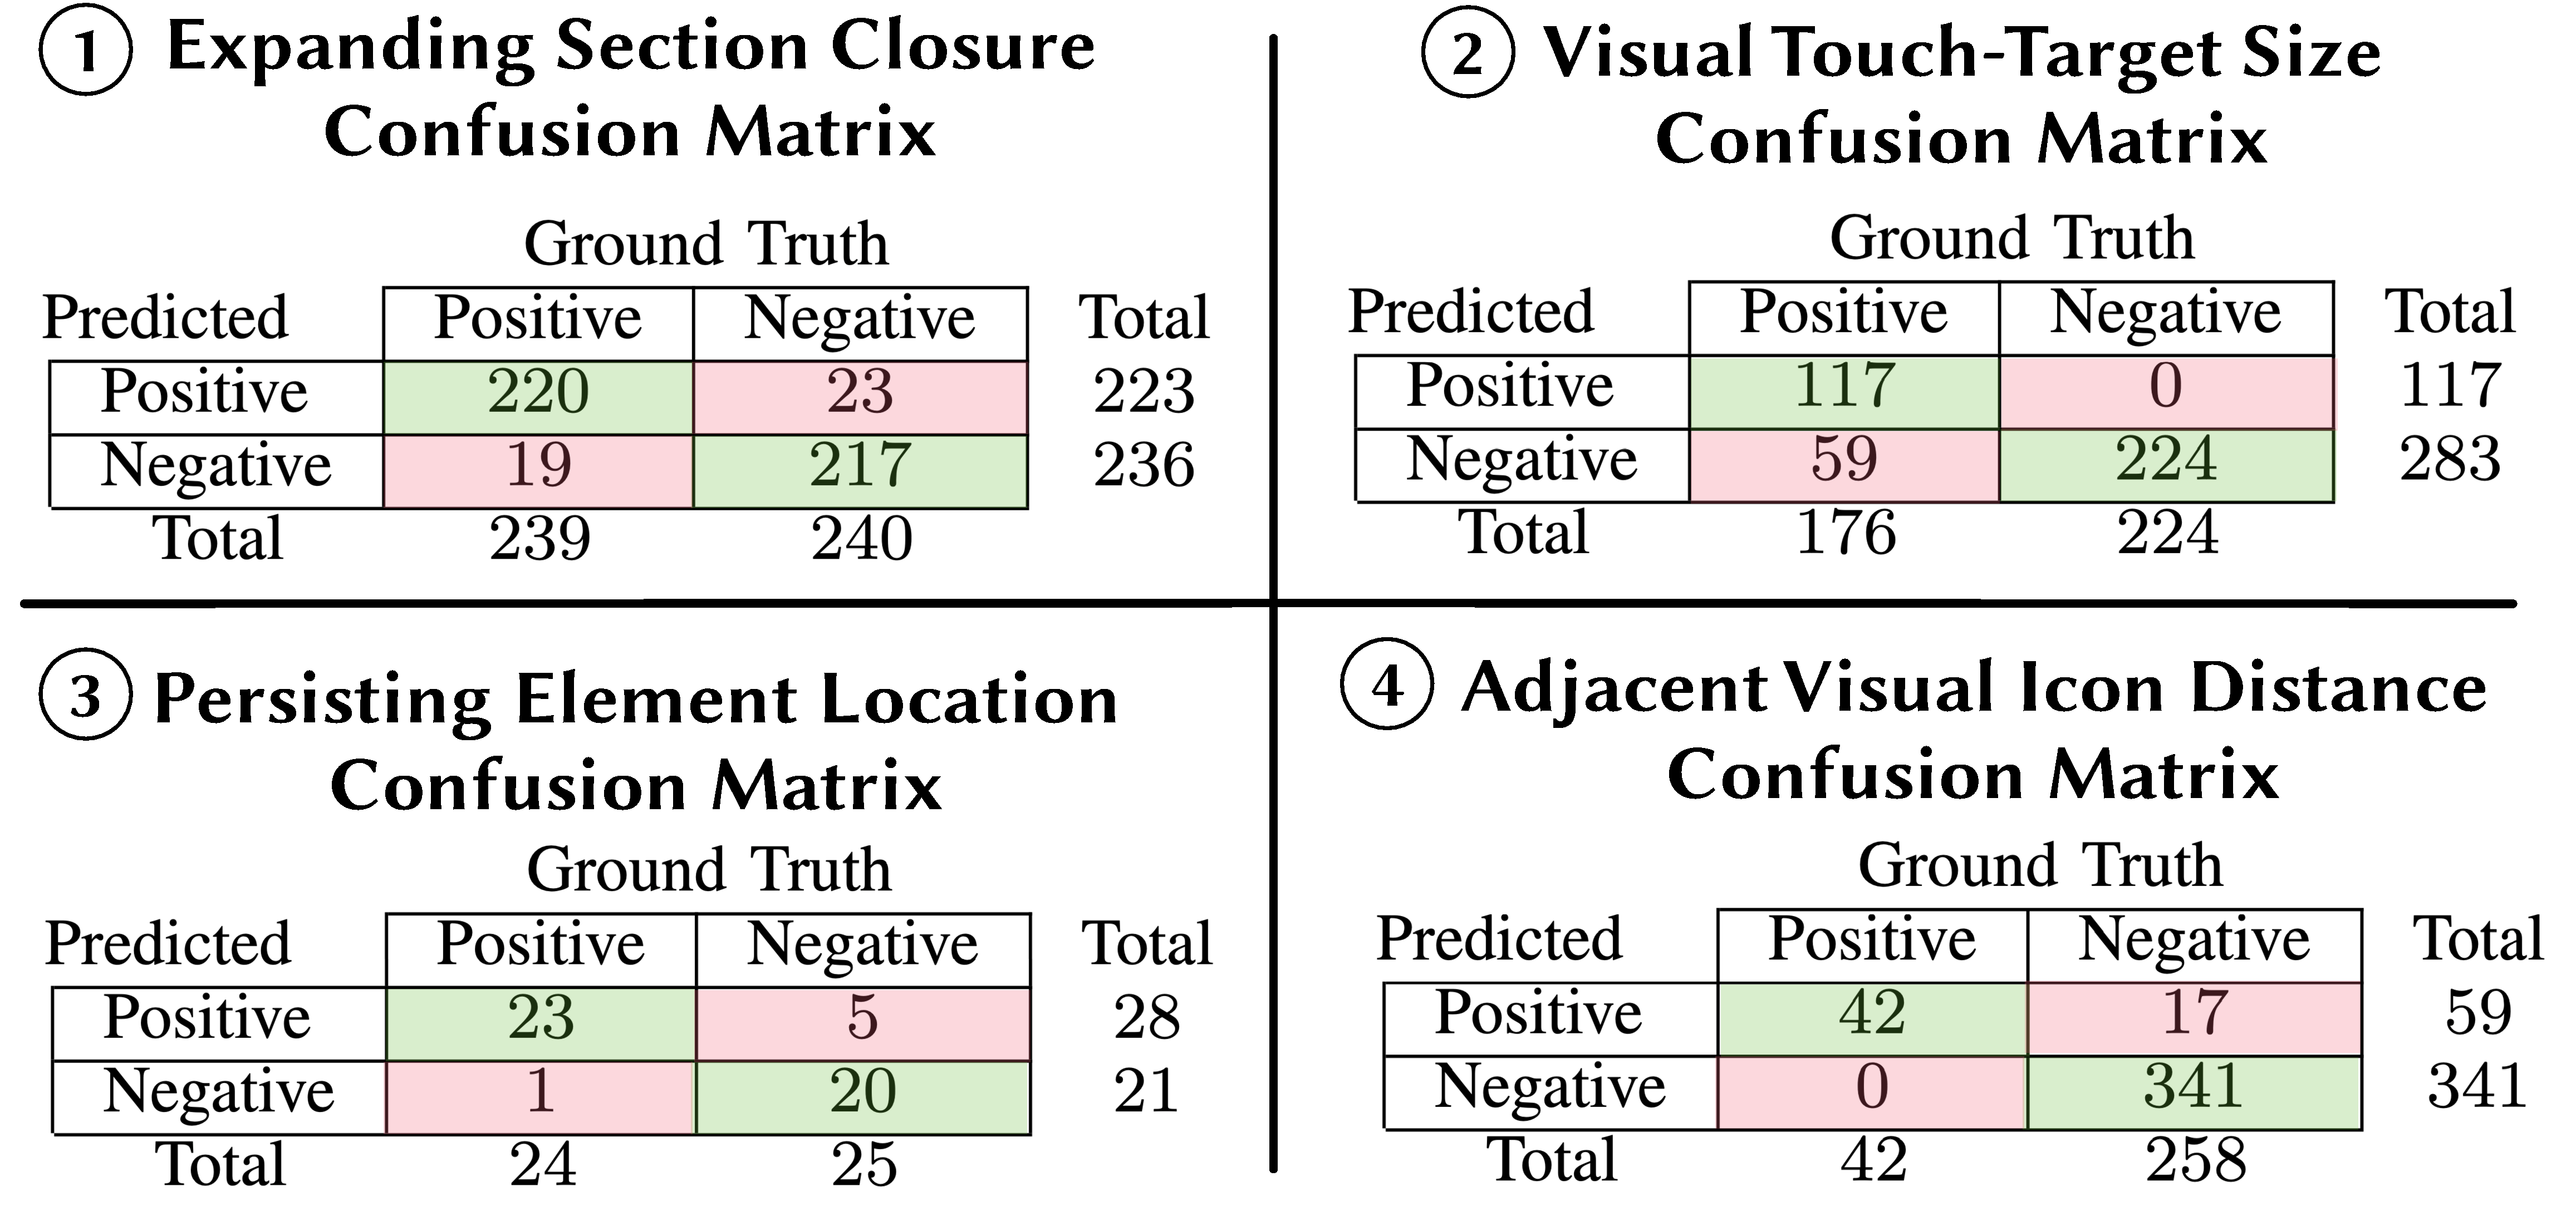
\includegraphics[width=0.75\textwidth]{imgs/confusion-matrices.pdf}
    \caption{Detector Confusion Matrices}
    \label{matrices}
\end{figure}

Figure~\ref{matrices}-\circled{2} illustrates that the visual touch target detector never produced a false-positive outcome. This is due to the fact that the detector specifically extracts elements labeled as clickable in the \texttt{\small XML}, therefore once they are extracted and have their edges analyzed, the detector is able to detect violations with certainty. The confusion matrix for the expanding section detector is shown in Figure~\ref{matrices}-\circled{1}, there were 23 false positive predictions, mainly due to limitations related to lexical pattern matching. Finally, \MotorEase's persisting element detector identified only 8 false positives, mainly due to inconsistencies in matching elements across screens due to unexpected changes in \texttt{\small uiautomator XML} files. In evaluating the effectiveness of \MotorEase, we also considered the impact of false negative predictions, as they signal violations that are not flagged by MotorEase, and hence could reach end-users. However, our evaluation revealed that the recall rate of \MotorEase was relatively high, indicating that it is a dependable tool with a high true positive rate, thus demonstrating its practical applicability.
In regards to \MotorEase's low false negative prediction rate, The confusion matrix analysis for the icon distance detector shown in Figure~\ref{matrices}-\circled{4} shows that \MotorEase predicted 0 false negatives. Moreover, the confusion matrix analysis for the persisting elements detector shown in Figure~\ref{matrices}-\circled{3} showed only one false negative prediction. Similarly, the confusion matrix for the expanding section detector presented in Figure~\ref{matrices}-\circled{1} demonstrated a false negative rate similar to its false positive rate, further supporting the viability of MotorEase. Overall, our evaluation demonstrates that \MotorEase is likely a generally practical tool, exhibiting a relatively low rate of false positives and negatives. % assisting developers in identifying as many motor-impairment accessibility issues as possible, while limiting the overhead imposed by false positive violations.
\MotorEase leverages it's ability to visually comprehend the visual and textual contents of a screen to determine accessibility violations. This approach offers distinct advantages. For instance, \MotorEase showcases its adaptability by effectively detecting accessibility guideline violations regardless of variations in UI design or format. In contrast, traditional metadata-based approaches might be limited in their ability to analyze physical elements on the screen. %making \MotorEase a more comprehensive solution.






\subsection{Accessibility Developer Tools Related Works}

This section will look at previous accessibility related research. Our approach introduces a novel way to determine motor accessibility guideline violations within apps. In our exploration for previous work, we found that motor impaired users were seldom the targeted demographic in accessibility testing research. We also discovered that testing for accessibility based on guidelines is a relatively young area of research with many open problems. However, previous work has been done in accessibility testing and is presented below.  

\subsubsection{Accessibility Studies on Mobile Apps}

There exists a large body of work that aims to understand how users with disabilities use their devices, and the potential accessibility issues that exist in current software applications~\cite{Mchugh20,Almeida10,Yan19,Silva20,Santiago22,Mateus20,Aizpurua14,Silva19,Oh13,Montague14}. Such studies tend to take two forms, user studies~\cite{Aizpurua14,Mateus20} and empirical analyses of software~\cite{Silva20,Yan19}.
Blind and low-vision users, like a majority of the population, have found themselves depending on their smartphones or touch screen devices recently \cite{Li22}.Touch devices have improved the life of people with disabilities, but some applications are still inaccessible to LV users \cite{Park14}. 
A study by Park et al. \cite{Park14} examined mobile application accessibility through a user study with four participants with an average of 1.9 years of experience with smartphones running IOS. The study aimed to produced a list of design guidelines for app developers to better support LV users some of which include text associations to UI elements, press action support (which is a way to make every interaction with a tap and no gestures), and under 30 items in a page \cite{Park14}. This study successfully produced a list of ten guidelines that the participants had the most issues with. 
The previous study looked at accessibility from an IOS standpoint and looked to create a set of guidelines for LV users \cite{Mateus20, Alshayban20, Kim16}. Alshayban et al. \cite{Alshayban20} examined the current state of accessibility issues in Android applications~\cite{Alshayban20} using a Google-provided accessibility testing framework~\cite{GoogleAccess},they found that Text Contrast, Touch Target, Image Contrast, and Speakable Text are the most frequent accessibility issues~\cite{Alshayban20}. 

Vendome et al. \cite{Vendome19} also examined the prevalence of accessibility issues in Android apps. In this study, the authors mined thousands of android applications and analyzed the usage of accessibility APIs and whether or not applications adhered to accepted guidelines. In addition, they mined thousands of messages on Stack Overflow and other interaction platforms to understand the sentiment of developers and the types of questions they were asking. They found that most accessibility based conversations were centered around LV features while a lesser number focused on DHH features. Surprisingly though, they found that accessibility APIs imported into the programs were used as a way to resolve non-accessibility issues such as, retrieving notifications from other apps or automating touch interactions in the device \cite{Vendome19}. 

Our approach is motivated by and complements what researchers have discovered in the above studies. These studies have shown the importance of the problem that \MotorEase tackles through illustrating the widespread prevalence of accessibility issues in mobile apps and illustrating a comparative lack of awareness of motor-impairment design guidelines and the needs of such users. Hence, these studies both motivate and validate our work on \MotorEase.

\vspace{-1em}
\subsubsection{Accessibility Testing}

Software testing for accessibility aids developers in identifying violations of guidelines set forth by companies and governments~\cite{Norman13, GoogleAccess, AppleAccess, Park14}. A wide range of research has been carried out to automate this process~\cite{Ramachandra18,Brajnik15,Salehnamadi21,axeray,Norman13,Eler18,Salehnamadi:ASE'22}. We discuss the most closely related approaches below.

Eler et.al. introduced the MATE tool~\cite{Eler18} that uses automated dynamic analysis to check for accessibility issues that affect users with visual impairments in mobile apps, and generate detailed reports that facilitate developers fixing identified issues. Similar to MATE, \MotorEase also leverages automated dynamic analysis and is able to generate reports that aid developers in fixing accessibility issues. However, our tool is differentiated by the ML-based analyses employed, and by it's focus on motor-impaired users.

Latte~\cite{Salehnamadi21} is an accessibility testing framework introduced by Salehnamadi et.al. for android applications that aims to provide a deeper analysis compared to testing frameworks provided by Google~\cite{ANDRDesign, GoogleAccess} by testing how accessibility services, such as VoiceOver, function in conjunction with feature-based use cases. The authors carried out an evaluation of their tool using the \texttt{\small switchAccess} and \texttt{\small TalkBack} services~\cite{AppleAccess, GoogleAccess} and found that several applications did not accommodate for both forms of accessible interactions. Latte is one of the only tools or studies that explicitly considers accessibility issues for users with motor impairments, given that it is capable of integrating with the \texttt{\small switchAccess} service in Android. However, given Latte's use case driven nature it both (1) requires pre-existing test cases, which many mobile apps have been shown to lack~\cite{Lin:ASE'20}, and (ii) cannot detect violations of the specific accessibility guidelines targeted by \MotorEase, as it attempts to carry out actions of a use case using an assistive service, and does not analyze the UI for specific patterns.  In short, \MotorEase and Latte serve largely \textit{complementary} purposes, that is \MotorEase provides UI design guidance to developers to avoid common pitfalls related to motor-impaired accessibility issues, and Latte can point out issues specific to given use cases and accessibility services. 

AXERAY~\cite{axeray} provides an accessibility testing tool that tests for accessibility design violations in web applications identified by prior work~\cite{Li22, Silva19, Almeida10}. This tool infers a semantic connection between different elements on the screen and attempts to group them together, then identifies whether the \texttt{\small HTML}/\texttt{\small CSS} markup on the page matches the semantic grouping. While \MotorEase shares some elements of the visual and textual analyses employed by AXERAY, it does so to target the detection of specific guideline violations, as opposed to forming semantic groups of UI elements. Furthermore, \MotorEase is focused on analyzing mobile apps as opposed to web apps, and is further focused specifically on accessibility issues that affect motor impaired users. We believe future work could translate techniques in this paper to the web domain.  

Chen et al. \cite{Chen22} introduced Xbot, an accessibility testing tool that is capable of identifying accessibility issues within an app using a combination of dynamic and static program analysis. Xbot is not able to uncover any of the accessibility issues targeted by \MotorEase. \MotorEase exhibits novelty as compared to Xbot as it  utilizes semantic understanding of the visual and textual elements of UI screens to detect new issues that affect motor-impaired users. 

Finally, recently Salehnamadi et.al introduced the Groundhog approach~\cite{Salehnamadi:ASE'22}, which is an accessibility crawler for mobile apps. Groundhog implements an automated UI crawler that explores an app both with and without assistive services, such as \texttt{\small TalkBack}, and notes any cases where an action can be performed through traditional touches, but cannot be performed via an assistive service. Again, \MotorEase is largely \textit{complementary} to this work, in that Groundhog targets general issues related to actionability and locatability of UI elements more broadly, but does not target the specific motor-impairment accessibility issues addressed by \MotorEase. In fact, \MotorEase aims to address two specific classes of issues identified in the Groundhog paper as being important for future work, (i) counterintuitive navigation (e.g., persisting elements) and (ii) inoperative actions (e.g., expanding sections).

\subsubsection{Accessibility-Based UI Comprehension}

%Developers and designers work to create UIs with able bodied users in mind, but they can violate accessibility guidelines or create cumbersome interfaces for users with disabilities \cite{Salehnamadi21, Li22, Bajammal21, Peng19}. 
Given that users interact with software through a UI, and past work has illustrated accessibility issues present in UIs~\cite{Salehnamadi21,Li22,Bajammal21,Peng19}, there is a body of work dedicated to automatically comprehending and augmenting UIs to identify and circumvent accessibility and UI issues~\cite{Liu21,Liu2021,Chen18,Gajos07,Shiver15,Montague12,Zhang21,Moran:ICSE'18,Moran:ASE'18}. %Below, we survey the most closely related work on UI comprehension and augmentation, differentiating \MotorEase in context. %There are two main areas of research being presented in this section GUI comprehension and GUI augmentation  . GUI comprehension, looks to dissect and understand the hierarchy of a GUI while GUI augmentation comprehends the UI and automatically changes elements to make a more accessible UI. Examples of previous research are presented below. 

UI elements and icons typically need to be labeled in order for screen readers to be able to properly describe their appearance and functionality, however, such metadata is often missing from apps~\cite{chen2020unblind}. Zhang et.al.\cite{Zhang21} and Chen et.al.~\cite{chen2020unblind} designed machine learning models trained from both existing UI labels and annotated labels from developers. %These approaches were found to be fairly accurate, with exact matches of labels on test sets eclipsing 60-70\% precision. 
Follow-up work by Mehralian et. al. introduced COALA~\cite{Mehralian:FSE'21}, which aimed to improve upon the automated icon labeling by considering context related to screen text and region to build a multi-modal model for predicting icon labels.

Mansur et.al. introduced the \AidUI~\cite{mansur2023aidui} tool, which uses semantic screen understanding to automatically identify and localize Dark Patterns in mobile app and web user interfaces. This technique uses similar techniques for semantic screen understanding as \MotorEase, but in different ways. For instance, while AidUI uses element size and distance between elements as a factor in determining certain dark patterns, \MotorEase aims to compare to the programmatic element size and visual element size to detect accessibility violations. Further, \MotorEase analyzes \textit{both} visual UI screenshots and \texttt{\small uiautomator} metadata, whereas AidUI operates only upon visual UI screenshots -- with the use of multimodal data serving as a source of novelty for \MotorEase.

Wu et al.~\cite{Wu21} developed a screen parser that is able to automatically reverse-engineer the hierarchical layout of elements a given UI screenshot using purely computer vision techniques. Chen et.al. developed a technique that uses multi-modal neural networks to generate a UI skeleton for mobile apps~\cite{Chen18}. Nguyen et.al.~\cite{Nguyen:ASE'15} and Moran et.al.~\cite{Moran:TSE'18} created approaches for automatically prototyping the UIs of applications using both supervised and unsupervised computer vision techniques to comprehend screen structure from pixels. While Wu et.al. illustrated that UI understanding and generation techniques could be used to bolster accessibility of mobile apps~\cite{Wu21}, these techniques target different accessibility issues as compared to \MotorEase. \


\subsection{Summary}
In this paper, we presented \MotorEase, an approach for detecting, classifying, reporting motor-impairment accessibility violations. We measured the performance, generalizability, and  applicability of \MotorEase to various open source applications. Our results indicate that \MotorEase is effective in practice and offers a novel approach for developers to identify accessibility issues affecting motor-impaired users. Future work will examine the potential to detect accessibility issues in web apps and conduct user~studies.














% 

% \section{FlakeFlagger: Flaky Test Classifier}
\label{sec:flakeFlaggerClassifier}

% \begin{table*}[t]
\scriptsize
%\renewcommand{\arraystretch}{1.3}
    \caption[FlakeFlagger List of Collected Features.]{Complete list of features captured for test flakiness prediction. The Covered Lines Churn feature is represented in multiple forms based on the $h$ values (number of the past commits). In the evaluation, I considered $h=5, 10, 25, 50, 75, 100, 500$ and $10,000$}
    \vspace{-5pt}
    \label{table:Feature_desc}
    \begin{tabularx}{\textwidth}{l | l X}
    \toprule
    & \bfseries Feature & \bfseries Description\\
    \midrule
\parbox[t]{2mm}{\multirow{8}{*}{\rotatebox[origin=c]{90}{Test Smells}}}	&
	Indirect Testing  	&	 True if the test interacts with the object under test via an intermediary \cite{van2001refactoring}  \\
	&	Eager Testing 	&	 True if the test exercises more than one method of the tested object \cite{van2001refactoring} \\
	&	Test Run War  	&	 True if the test allocates a file or resource which might be used by other tests \cite{van2001refactoring} \\
	&	Conditional Logic 	&	 True if the test has a conditional if-statement within the test method body \cite{meszaros2007xunit} \\
	&	Fire and Forget  	&	 True if the test launches background threads or tasks. \cite{garousi2018smells} \\
	&	Mystery Guest 	&	 True if the test accesses external resources  \cite{van2001refactoring} \\
	&	Assertion Roulette  	&	 True if the test has multiple assertions \cite{van2001refactoring} \\
	&	Resources Optimism  	&	 True if the test accesses external resources without checking their availability \cite{van2001refactoring}\\ \hline
\parbox[t]{2mm}{\multirow{8}{*}{\rotatebox[origin=c]{90}{Numeric Features}}}	&	Test Lines of Code   	&	 Number of lines of code in the test method body \\
	&	Number  of Assertions  	&	 Number of assertions checked by the test \\
	&	Execution Time   	&	 Running time for the test execution \\
	&	Source Covered Lines  	&	 Number of lines covered by each test, counting only production code \\
	&	Covered Lines  	&	 Total number of lines of code covered by the test  \\
	&	Source Covered Classes  	&	 Total number of production classes covered by each test \\
	&	External Libraries  	&	 Number of external libraries used by the test \\
	&	Covered Lines Churn 	&	 $h$-index capturing churn of covered lines in past 5, 10, 25, 50, 75, 100, 500, and 10,000 commits. Each value $h$ indicates that at least $h$ lines were modified at least $h$ times in that period.\\
\bottomrule
    \end{tabularx}
    % \vspace{-14pt}
\end{table*}

% \begin{table*}[t]
% \begin{tabular}{l l l}
% & Indirect Test Smell & Testing blah\\
% \end{tabular}
% \end{table*}

\begin{figure*}[t]
%\captionsetup{singlelinecheck = false, justification=justified}
  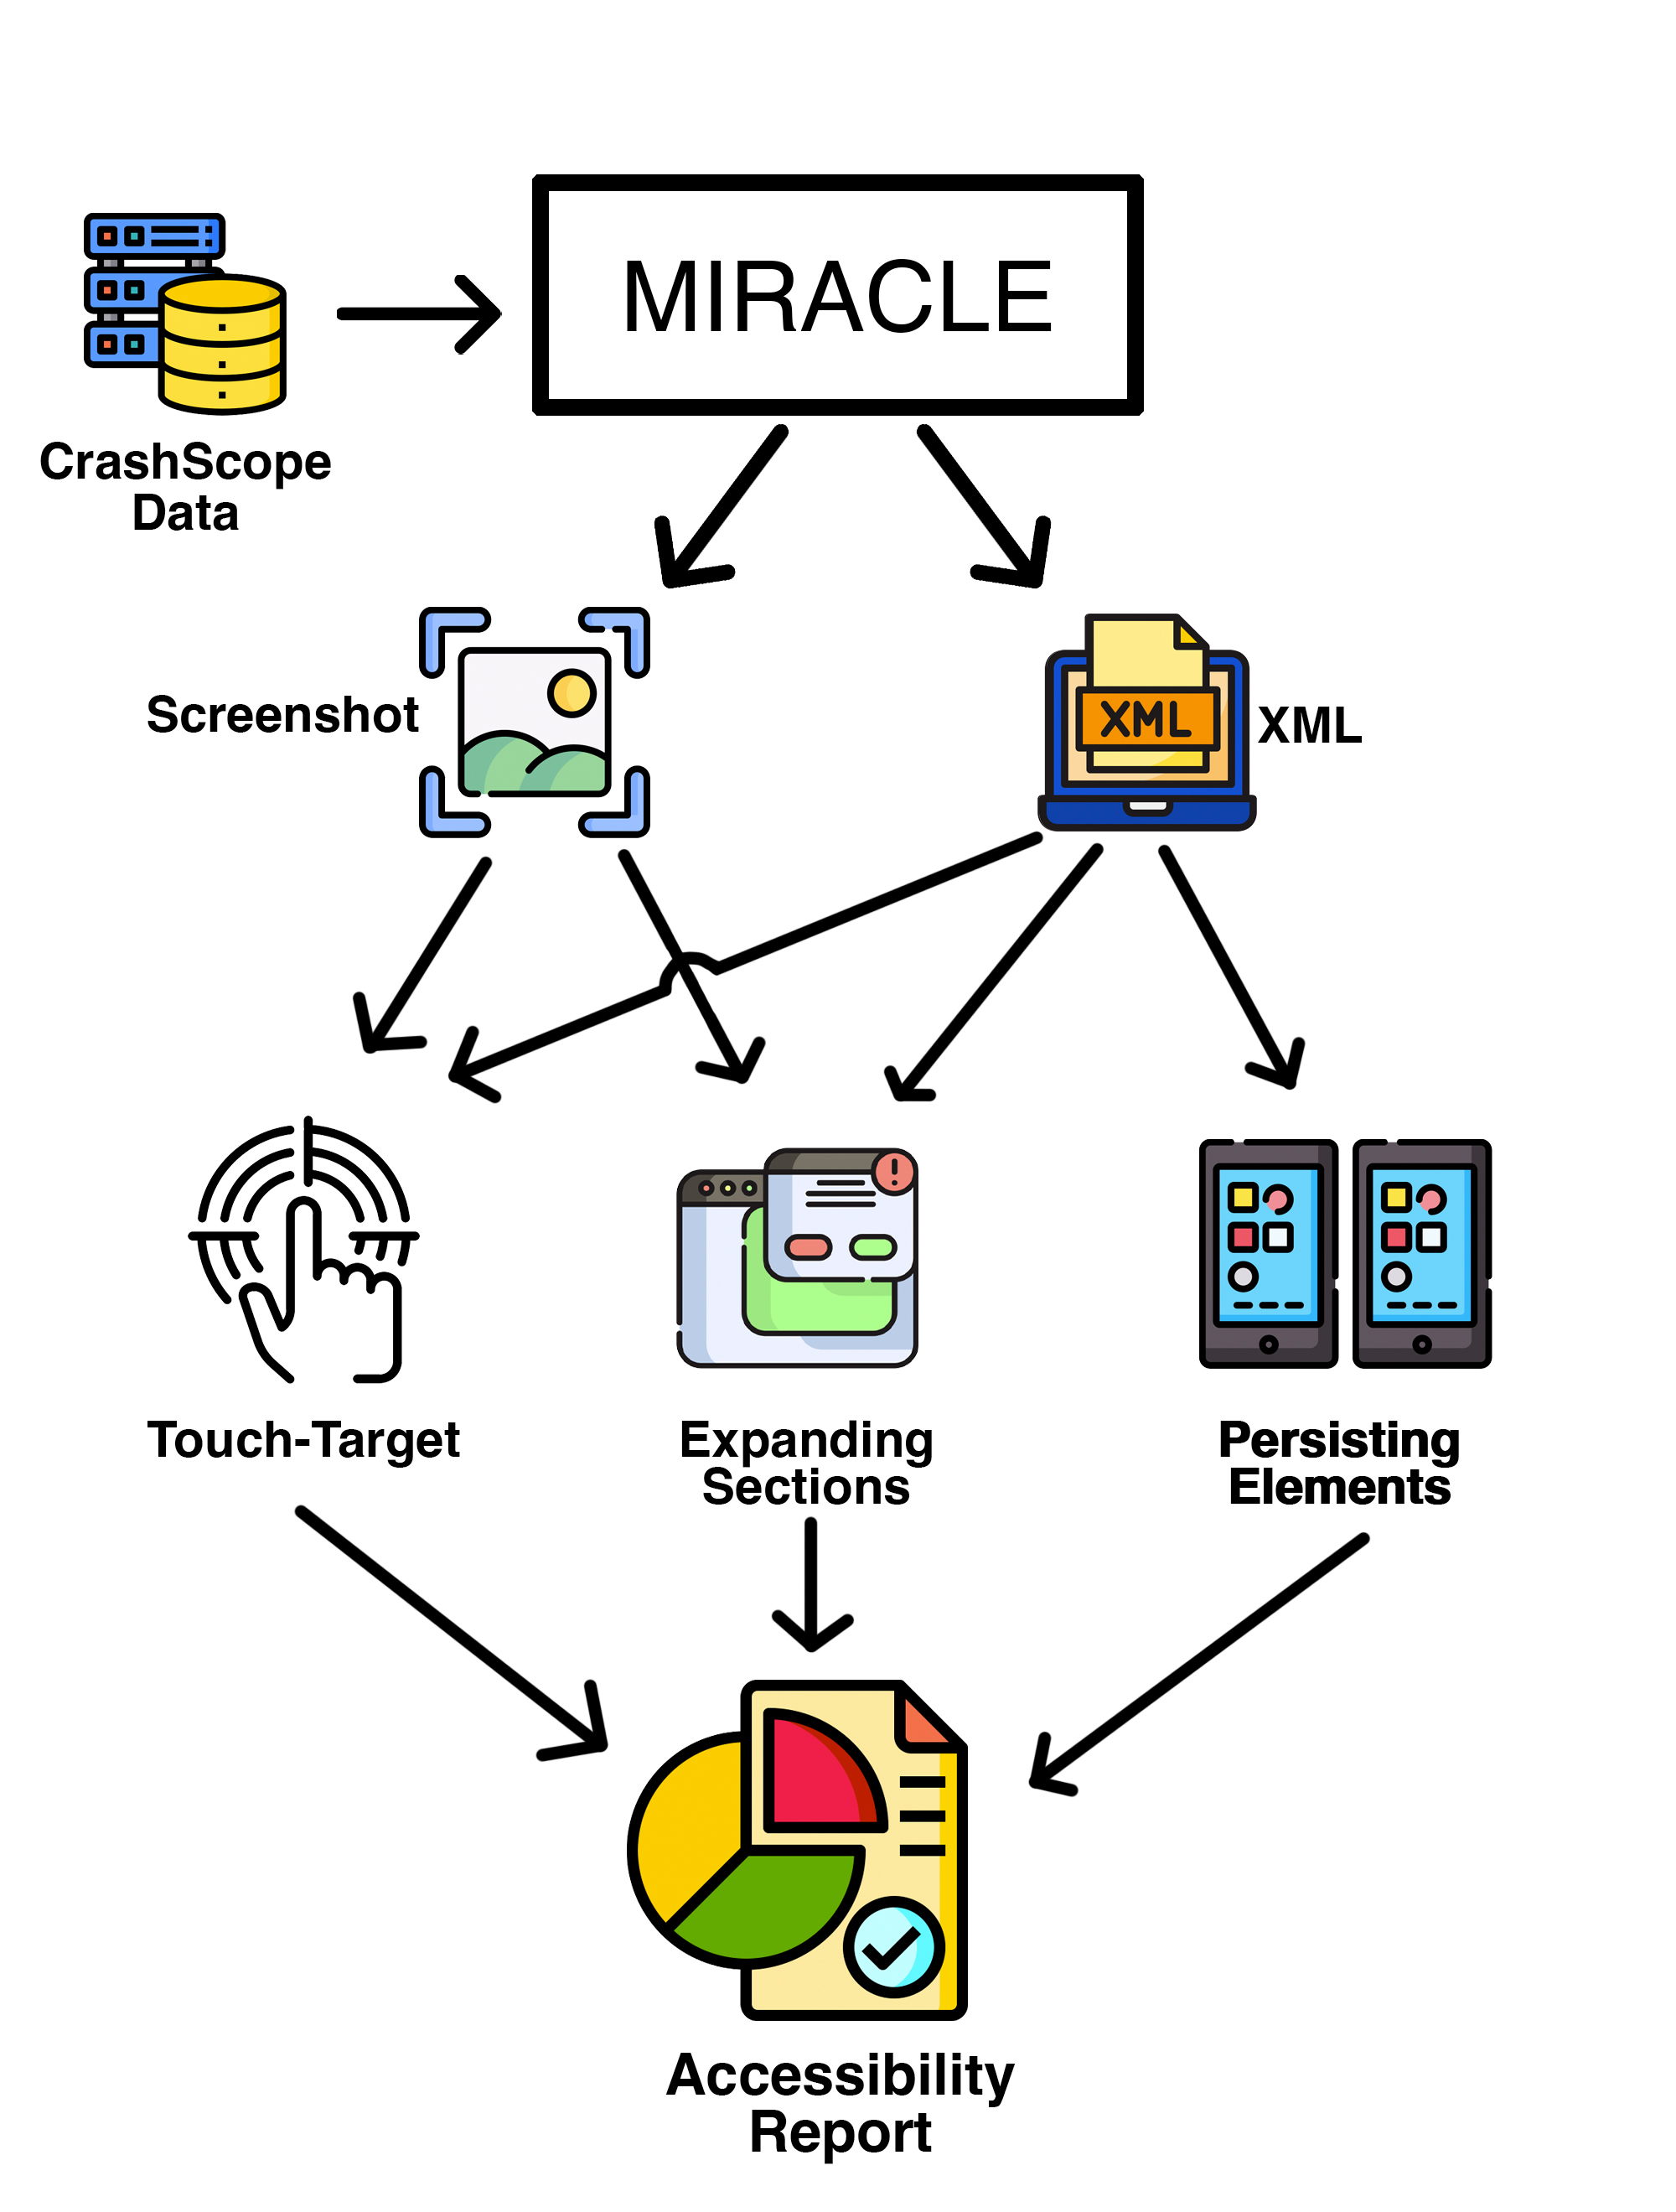
\includegraphics[width=0.9\textwidth]{Figures/overview.pdf}
  \centering
  \vspace{-5pt}
  \caption{Overview of \sysName's approach to predict likely flaky tests given a set of known flaky tests.}
  \vspace{-15pt}
  \label{over_all_graph}
\end{figure*}
\vspace{-5pt}

This section is a summary of the \emph{approach} section in my paper ``FlakeFlagger: Predicting Flakiness Without Rerunning Tests" published in ICSE2021 \cite{alshammari2021flakeflagger}.

\sysName is a Machine Learning (ML) approach to identify which tests in a test suite are flaky, \emph{without} rerunning them many times. \sysName learns from existing flaky tests in order to predict unseen tests if they are flaky or not. \sysName can be used to search for flaky tests in a large test suite, where developers identify that a portion of the test suite is or is not flaky, and use \sysName to help label the rest of the tests as flaky or not. Also, \sysName could help in terms \emph{prioritize} which tests should be run first by reporting which tests are most likely to be flaky. 


By proactively identifying flaky tests, we may also help developers understand why these tests are flaky.
Prior work has suggested different properties of tests that might make them more likely to be flaky, and \sysName can report which of these features are present in each test~\cite{eck2019understanding,ahmad2021empirical}.
In practice, if a feature has a strong correlation with flakiness, developers might choose to focus on this feature in their future test maintenance and development activities. 





\subsection{Features Collections}
\label{sec:detector}
Machine learning classifiers such as \sysName require a set of feature in order to learn and predict. I started with the prior work \cite{luo2014empirical,eck2019understanding,bell2018deflaker} to study which features is highly linked to flakiness. I aim to collect verity of features because of the fact that some flaky tests in different projects often have different root causes for their flakiness\cite{luo2014empirical}. Similarly, some features that are predictive for one project may not be as predictive for others, due to the inherent non-determinism in flaky tests. 
I intentionally collect some dynamic features, in addition to static features (e.g. presence of textual tokens in the body of each test method). This is important because some causes not in the test method itself, but instead, in the production code that is executed by that test \cite{eck2019understanding}.
Ahmed et al. \cite{ahmad2021empirical} categorized 23 developer-reported factors which affect test flakiness. 
These features are described by practitioners at a high level, and include test case complexity, hard-coded values and test smells.
Eck et al. \cite{eck2019understanding} interviewed 21\Space{ professional} developers about flaky tests and tabulated the frequency of different kinds of flaky tests as well as developers' fixes for those flaky tests. 


Inspired by previous studies on test flakiness, I developed a list of sixteen features, 
some of are based on general studies on the causes of flaky tests \cite{luo2014empirical,ahmad2021empirical}, while others are defined as bad practices in writing unit tests.
Hence, I considered all of the features described in the prior works, and then selected only those for which I could write automated detectors.
This ends up with implementing detectors for each of the features shown in Table \ref{table:Feature_desc}. This list of features is not intended to be complete: there may yet be other features that can be easily collected and will be useful for predicting test flakiness.

While some of the features can be detected by inspecting the test method statically (specifically, the conditional logic smell and test line of code), the rest of the features require more than static analysis.
A hybrid static/dynamic framework \emph{detector} was developed to collect the statement coverage of each test, and then statically analyze the covered code in order to collect these behavioral features.
The \emph{detector} also collect a variety of other features related to the statement coverage of each test, such as how many recently changed lines of code are covered.
The \emph{detector} is implemented as an extension to the Maven build system.



\subsection{Classification Process}

FlakeFlagger takes a list of tests, where each of them is represented as a vector $\{x_1, x_2, x_3,\dots, x_n\}$  where each \emph{x} represents a feature value and \emph{n} correspond the total number of features. I applied data inspection and cleaning process to make that dataset more clear for the classification. Missing data can exist to the dataset due to the fact that some features collected by the detector can be incomplete e.g. due to crashes in the middle of the test execution. Some tests are not written in Java, and hence the feature detectors may not be applicable to them, and due to inheritance, some tests may not have source code in the project under test.

As in any classification problem, considering multiple supervised learning algorithms could be better. In \sysName, it is designed to use a set of models including Random Forest (\emph{RF}) and Decision Tree (\emph{DT}. I follow a feature selection process using \emph{information gain}, which computes the amount of information that a feature can provide for a classification \cite{lei2012feature}. Imbalanced datasets (where there is not an equal number of instances in each class --- flaky and non-flaky tests in our case) usually have very low information gain values. 


\subsection{Experimental Design}
\label{sec:Prediction_Design}
To evaluate \sysName, I used the same dataset described in Section \ref{sec:flakeFlaggerStudy}. I ran the detector described in Section \ref{sec:detector}, to collect the set of features shown in Table \ref{table:Feature_desc}. \sysName, similar to any machine learning classifiers, relies on two data sets: one to build the model (training) and another for testing. Because this is not already designed and I have only one dataset, I applied $k$-fold cross validation  \cite{kohavi1995study,bengio2004no} to evaluate our model. Following this practice, we split the data into $k$ parts, leave one part for testing and $k-1$ to train the classifier.
We then repeat this process with another $k-1$ parts, each time leaving one part for testing.
However, $k$-fold cross validation is most applicable to data that is evenly balanced, where the proportions of each class (flaky and not flaky) are similar. In fact, most tests are not flaky, which means imbalance data. To overcome this, I applied a sample technique SMOTE \cite{chawla2002smote} only on training dataset, to ensure a valid and fair result.




%  the new table 3 

\begin{table*}[t]
 \setlength{\tabcolsep}{1.6pt}

\caption[FlakeFlagger Prediction Result.]{Prediction performance for \sysName, the \vocabName, and the hybrid combination of both.
\textnormal{The hybrid approach builds a model with both \sysName's and the \vocabName's features. I show the number of True Positives, False Negatives, False Positives and True Negatives, Precision, Recall, and F1 scores per-project.
The AUC value is calculated after each fold where the reported value is the overall averages of AUC values after all folds. Projects with zero F1 values have very low numbers of flaky tests (less than 3 per project), and illustrate known limitations of \sysName. } }
%\caption{Prediction performance for \sysName, MSR and the combination between two approaches. 
% \textnormal{For \sysName, showing True Positives, False Negatives, False Positives, True Negatives, Precision, Recall and F1-score. For comparison approaches (FLAST \cite{flast} at $\sigma=0.5$ and $\sigma=0.95$ and random guessing with 50\% probability of flakiness or weighted by the distribution of flaky tests in the project), we show only Precision, Recall and F1-score. Highest F1-score in each row is shown in bold. Since each project uses a different model, we do \emph{not} include a ``total'' row.}
%}
\label{table:Full_result}
\vspace{-5pt}
\resizebox{\textwidth}{!}{
% \scriptsize
\begin{tabular}{l rr| rrrrrrr | rrrrrrr | rrrrrrr}

\toprule
% & \multicolumn{4}{c|}{} & \multicolumn{4}{c|}{\textbf{MSR tool *}} & \multicolumn{4}{c}{\textbf{Both}}\\
% \cmidrule(lr){2-5} \cmidrule(lr){6-10}
& & \textbf{Flaky by} & \multicolumn{7}{c|}{\textbf{\sysName}} & \multicolumn{7}{c|}{\textbf{Vocabulary-Based Approach \cite{pintovocabulary}}} & \multicolumn{7}{c}{\textbf{Combined Approach}}  \\
\cmidrule(lr){4-10} \cmidrule(lr){11-17}  \cmidrule(lr){18-24}
% \cmidrule(lr){2-14} \cmidrule(lr){10-13} \cmidrule(lr){14-17} \cmidrule(lr){18-21} 


\textbf{Project} & \textbf{Tests} & \textbf{Reruns} &\textbf{TP} & \textbf{FN} & \textbf{FP} & \textbf{TN} & \textbf{Pr} & \textbf{R} & \textbf{F} & \textbf{TP} & \textbf{FN} & \textbf{FP} & \textbf{TN} & \textbf{Pr} & \textbf{R} & \textbf{F} &  \textbf{TP} & \textbf{FN} & \textbf{FP} & \textbf{TN} & \textbf{Pr} & \textbf{R} & \textbf{F}\\
\midrule
spring-boot& 2,108 & 160 & 139 & 21 & 15 & 1,933 & 90\% & 87\% & 89\% & 134 & 26 & 703 & 1,245 & 16\% & 84\% & 27\% & 143 & 17 & 18 & 1,930 & 89\% & 89\% & 89\% \\
\rowHighlight hbase &431 & 145& 129 & 16 & 32 & 254 & 80\% & 89\% & 84\% & 89 & 56 & 152 & 134 & 37\% & 61\% & 46\% & 130 & 15 & 33 & 253 & 80\% & 90\% & 84\% \\
alluxio & 187 & 116& 116 & 0 & 0 & 71 & 100\% & 100\% & 100\% & 108 & 8 & 11 & 60 & 91\% & 93\% & 92\% & 116 & 0 & 0 & 71 & 100\% & 100\% & 100\% \\
\rowHighlight okhttp & 810 &100 & 52 & 48 & 159 & 551 & 25\% & 52\% & 33\% & 79 & 21 & 444 & 266 & 15\% & 79\% & 25\% & 46 & 54 & 104 & 606 & 31\% & 46\% & 37\% \\
ambari & 324 & 52& 47 & 5 & 3 & 269 & 94\% & 90\% & 92\% & 36 & 16 & 121 & 151 & 23\% & 69\% & 34\% & 47 & 5 & 3 & 269 & 94\% & 90\% & 92\% \\
\rowHighlight hector & 142 & 33 & 30 & 3 & 8 & 101 & 79\% & 91\% & 85\% & 13 & 20 & 23 & 86 & 36\% & 39\% & 38\% & 25 & 8 & 11 & 98 & 69\% & 76\% & 72\% \\
activiti & 2,043 & 32 & 10 & 22 & 43 & 1,968 & 19\% & 31\% & 24\% & 12 & 20 & 531 & 1,480 & 2\% & 38\% & 4\% & 7 & 25 & 34 & 1,977 & 17\% & 22\% & 19\% \\
\rowHighlight java-websocket & 145 & 23& 19 & 4 & 1 & 121 & 95\% & 83\% & 88\% & 23 & 0 & 74 & 48 & 24\% & 100\% & 38\% & 19 & 4 & 4 & 118 & 83\% & 83\% & 83\% \\
wildfly &1,023 & 23 & 11 & 12 & 27 & 973 & 29\% & 48\% & 36\% & 20 & 3 & 554 & 446 & 3\% & 87\% & 7\% & 17 & 6 & 24 & 976 & 41\% & 74\% & 53\% \\
\rowHighlight httpcore & 712 & 22& 14 & 8 & 23 & 667 & 38\% & 64\% & 47\% & 16 & 6 & 375 & 315 & 4\% & 73\% & 8\% & 15 & 7 & 24 & 666 & 38\% & 68\% & 49\% \\
logback & 805 & 22& 3 & 19 & 17 & 766 & 15\% & 14\% & 14\% & 10 & 12 & 259 & 524 & 4\% & 45\% & 7\% & 5 & 17 & 11 & 772 & 31\% & 23\% & 26\% \\
\rowHighlight incubator-dubbo & 2,174 & 19& 8 & 11 & 35 & 2,120 & 19\% & 42\% & 26\% & 11 & 8 & 813 & 1,342 & 1\% & 58\% & 3\% & 13 & 6 & 23 & 2,132 & 36\% & 68\% & 47\% \\
http-request & 163 & 18& 12 & 6 & 6 & 139 & 67\% & 67\% & 67\% & 16 & 2 & 84 & 61 & 16\% & 89\% & 27\% & 12 & 6 & 6 & 139 & 67\% & 67\% & 67\% \\
\rowHighlight wro4j & 1,135 & 16 & 4 & 12 & 2 & 1,117 & 67\% & 25\% & 36\% & 2 & 14 & 101 & 1,018 & 2\% & 12\% & 3\% & 0 & 16 & 1 & 1,118 & 0\% & 0\% & 0\% \\
orbit & 86 & 7& 1 & 6 & 8 & 71 & 11\% & 14\% & 12\% & 6 & 1 & 32 & 47 & 16\% & 86\% & 27\% & 1 & 6 & 7 & 72 & 12\% & 14\% & 13\% \\
\rowHighlight undertow & 183 & 7& 2 & 5 & 8 & 168 & 20\% & 29\% & 24\% & 6 & 1 & 63 & 113 & 9\% & 86\% & 16\% & 3 & 4 & 8 & 168 & 27\% & 43\% & 33\% \\
achilles &1,317 & 4 & 2 & 2 & 3 & 1,310 & 40\% & 50\% & 44\% & 0 & 4 & 0 & 1,313 & 0\% & 0\% & 0\% & 0 & 4 & 0 & 1,313 & 0\% & 0\% & 0\% \\
\rowHighlight elastic-job-lite & 558 &3 & 0 & 3 & 0 & 555 & 0\% & 0\% & 0\% & 0 & 3 & 34 & 521 & 0\% & 0\% & 0\% & 1 & 2 & 0 & 555 & 100\% & 33\% & 50\% \\
zxing & 345 & 2 & 0 & 2 & 2 & 341 & 0\% & 0\% & 0\% & 1 & 1 & 144 & 199 & 1\% & 50\% & 1\% & 0 & 2 & 2 & 341 & 0\% & 0\% & 0\% \\
\rowHighlight assertj-core & 6,261 & 1& 0 & 1 & 5 & 6,255 & 0\% & 0\% & 0\% & 0 & 1 & 6 & 6,254 & 0\% & 0\% & 0\% & 0 & 1 & 0 & 6,260 & 0\% & 0\% & 0\% \\
commons-exec & 55 & 1& 0 & 1 & 1 & 53 & 0\% & 0\% & 0\% & 1 & 0 & 18 & 36 & 5\% & 100\% & 10\% & 0 & 1 & 1 & 53 & 0\% & 0\% & 0\% \\
\rowHighlight handlebars.java & 420 & 1& 0 & 1 & 5 & 414 & 0\% & 0\% & 0\% & 0 & 1 & 91 & 328 & 0\% & 0\% & 0\% & 0 & 1 & 0 & 419 & 0\% & 0\% & 0\% \\
ninja &307 &1 & 0 & 1 & 3 & 303 & 0\% & 0\% & 0\% & 0 & 1 & 50 & 256 & 0\% & 0\% & 0\% & 0 & 1 & 0 & 306 & 0\% & 0\% & 0\% \\

\midrule
\rowHighlight \textbf{Total} & 21,734 & 808 & 599 & 209 & 406 & 20,520 & 60\%& 74\%& 66\%&  583 & 225 & 4,683 & 16,243 & 11\%& 72\%& 19\%& 600 & 208 & 314 & 20,612& 66\%& 74\%& 68\% \\
\midrule
% \textbf{Precision} &&& \multicolumn{7}{c|}{60\%} & \multicolumn{7}{c|}{11\%} & \multicolumn{7}{c}{66\%} \\
% \textbf{Recall} &&& \multicolumn{7}{c|}{74\%} & \multicolumn{7}{c|}{72\%} & \multicolumn{7}{c}{74\%} \\
% \textbf{F1-score} &&& \multicolumn{7}{c|}{66\%} & \multicolumn{7}{c|}{19\%} & \multicolumn{7}{c}{70\%} \\
% \textbf{AUC} (Average per fold) &&& \multicolumn{7}{c|}{86\%} & \multicolumn{7}{c|}{75\%} & \multicolumn{7}{c}{68\%}\\ \bottomrule	
\end{tabular}}
\vspace{-15pt}
\end{table*}



In our prediction evaluation, I label each prediction result as a True Positive (TP), False Negative (FN), False Positive (FP), or True Negative (TN) as follows:
TP - predicted flaky, known to be flaky; FP - predicted flaky, not known to be flaky; FN - predicted not flaky, known to be flaky; TN - predicted not flaky, not known to be flaky.
I also evaluate our models using F1-score, which is computed using the standard formula based on Recall and Precision. %, to evaluate how our approach works to detect flaky tests as $TP$s.
%  \abdul{I added the following sentences ... } JB: Looks good!
Lastly, I calculate the Area Under the Curve (AUC), a measure of how effective a model is at distinguishing classes (in our case, flaky and not flaky).

In the evaluation, false positives represent the number of tests that might be considered as flaky by developers, resulting in excess effort spent re-running them to determine if they are flaky or not. I focus primarily on total positives, because I have confidence that the collected flaky tests are indeed flaky, but I cannot be confident in our classification of a test as not flaky. 
In other words, the oracle is a result of detecting flaky tests after \numruns~runs for each test, but this does not guarantee that the ``not flaky'' tests are really not flaky: they may just not have been observed to be flaky. 
This approach also allows us to confirm $FN$s are truly flaky tests because they fail at least once during rerun tests.
However, because of the inherent non-determinism in flaky tests, I cannot construct a reliable oracle to evaluate $TN$s and $FP$s, but report them as-is.



\begin{table*}[t]
\scriptsize
%\renewcommand{\arraystretch}{1.3}
    \caption[FlakeFlagger List of Collected Features.]{Complete list of features captured for test flakiness prediction. The Covered Lines Churn feature is represented in multiple forms based on the $h$ values (number of the past commits). In the evaluation, I considered $h=5, 10, 25, 50, 75, 100, 500$ and $10,000$}
    \vspace{-5pt}
    \label{table:Feature_desc}
    \begin{tabularx}{\textwidth}{l | l X}
    \toprule
    & \bfseries Feature & \bfseries Description\\
    \midrule
\parbox[t]{2mm}{\multirow{8}{*}{\rotatebox[origin=c]{90}{Test Smells}}}	&
	Indirect Testing  	&	 True if the test interacts with the object under test via an intermediary \cite{van2001refactoring}  \\
	&	Eager Testing 	&	 True if the test exercises more than one method of the tested object \cite{van2001refactoring} \\
	&	Test Run War  	&	 True if the test allocates a file or resource which might be used by other tests \cite{van2001refactoring} \\
	&	Conditional Logic 	&	 True if the test has a conditional if-statement within the test method body \cite{meszaros2007xunit} \\
	&	Fire and Forget  	&	 True if the test launches background threads or tasks. \cite{garousi2018smells} \\
	&	Mystery Guest 	&	 True if the test accesses external resources  \cite{van2001refactoring} \\
	&	Assertion Roulette  	&	 True if the test has multiple assertions \cite{van2001refactoring} \\
	&	Resources Optimism  	&	 True if the test accesses external resources without checking their availability \cite{van2001refactoring}\\ \hline
\parbox[t]{2mm}{\multirow{8}{*}{\rotatebox[origin=c]{90}{Numeric Features}}}	&	Test Lines of Code   	&	 Number of lines of code in the test method body \\
	&	Number  of Assertions  	&	 Number of assertions checked by the test \\
	&	Execution Time   	&	 Running time for the test execution \\
	&	Source Covered Lines  	&	 Number of lines covered by each test, counting only production code \\
	&	Covered Lines  	&	 Total number of lines of code covered by the test  \\
	&	Source Covered Classes  	&	 Total number of production classes covered by each test \\
	&	External Libraries  	&	 Number of external libraries used by the test \\
	&	Covered Lines Churn 	&	 $h$-index capturing churn of covered lines in past 5, 10, 25, 50, 75, 100, 500, and 10,000 commits. Each value $h$ indicates that at least $h$ lines were modified at least $h$ times in that period.\\
\bottomrule
    \end{tabularx}
    % \vspace{-14pt}
\end{table*}

% \begin{table*}[t]
% \begin{tabular}{l l l}
% & Indirect Test Smell & Testing blah\\
% \end{tabular}
% \end{table*}


\subsection{Evaluation}
I evaluate the FlakeFlagger classifier by answering the following two main research questions:


\begin{description}
  \item[\textbf{RQ1:}] How effective is \sysName at predicting flaky tests?
  \item[\textbf{RQ2:}] How helpful is each feature in distinguishing between flaky and non flaky tests?

 \end{description}

\textbf{RQ1.} I used the results from rerunning tests (Section \ref{sec:flakeFlaggerStudy}) as the oracle for \sysName classification process, and ran the feature detector once on each of the same tests in order to gather the data needed to build a model.
I considered several different approaches to process the data, and measure classifier performance with a confusion matrix, precision, recall, F1-score and AUC. Even I applied different classification algorithms and balance techniques, I found that the best prefroamcne was  random forest model built using the SMOTE technique for balancing the training data (and using unbalanced testing data). I compare the result of \sysName classifier with the one of the state-of-the-art flaky test classifier, a \vocabName proposed by Pinto et al.~\cite{pinto2020vocabulary} which extracts tokens from each test using a simple bag-of-words model. I considered a hybrid model that adds the token features to \sysName's features. I consider only projects that have at least 10 flaky tests to ensure as shown in Table \ref{table:Full_result}. 

Overall, \sysName and the \vocabName  both detected a very similar number of flaky tests (599 and 583 respectively, out of a total of 808 flaky tests), but the two approaches varied in terms of precision --- \sysName had a far lower false positive rate with just \flaggerfp, compared to \msrfp~false positives from the \vocabName. Considering the initial use-case of a researcher or developer using \sysName to determine which tests to run time-intensive flaky test detectors on, using either \sysName or the \vocabName would result the same number of flaky tests eventually detected (that is, both have comparable recall).
However, if a developer uses both models to detect tests that are most likely to be flaky (which are false positive tests), \sysName reports fewer rate than \vocabName (406 vs 4,683).

\sysName's performance varied across projects: some projects (e.g., alluxio), had perfect precision and recall, while on others (e.g., okhttp and activiti) the approach was less successful. I investigated more about the results per projects and the performance could vary due to many reasons. First, the training and testing dataset sizes vary from one project to another. Because each project has its own environmental assumptions, development patterns, and other unique characteristics, it is really difficult to create a single general-purpose approach for flakiness classifications. Another reason for why performance varies across projects may be that not all flaky tests have been labeled correctly --- no rerun-based technique can guarantee to find all flaky tests (even after 10,000 reruns). The higher number of observed flaky tests in a single project does not guarantee that \sysName performs well.
Some flaky failures are due to rare dependency conflicts and network failures that are not captured well from our features described in Table \ref{table:Feature_desc}.
For example, okhttp has a high number of false positives and false negatives. With a further inspection on this particular project, there is a group of tests had all failed in the same way due to the same dependency problem in one single run.



\begin{table}[t]
\centering
  \setlength{\tabcolsep}{5.0pt}

\caption{\centering{Information gain (IG) for \sysName and the \vocabName.}}

\label{table:tokenbyig}
\vspace{-4pt}
%\resizebox{\t  extwidth}{!}{
\scriptsize
\begin{tabular}{lr|lr}

\toprule
\multicolumn{2}{c|}{\textbf{Vocabulary-Based Features}} & \multicolumn{2}{c}{\textbf{\sysName Features}}  \\
\cmidrule(lr){1-2} \cmidrule(lr){3-4}  


\textbf{Feature/Token} & \textbf{IG} & \textbf{Feature} & \textbf{IG} \\
\midrule

Test Lines of Code & 0.023 & Execution Time & 0.121 \\
\rowHighlight throws & 0.022 & Source Covered Lines & 0.067 \\
should & 0.020 & Source Covered Classes & 0.057 \\
\rowHighlight exception & 0.018 & Covered Lines & 0.034 \\
mtfs & 0.018 & Covered Changes (past 75 commits) & 0.029 \\
\rowHighlight runbuildfortask & 0.017 & Covered Changes (past 50 commits) & 0.028 \\
tfs & 0.017 & Covered Changes (past 100 commits) & 0.028 \\
\rowHighlight run & 0.016 & Covered Changes (past 500 commits) & 0.024 \\
transitive & 0.016 & Test Lines of Code & 0.023 \\
\rowHighlight ioexception & 0.015 & Covered Changes (past 10 commits) & 0.018 \\
tachyon & 0.014 & Covered Changes (past 1000 commits) & 0.015 \\
\rowHighlight fileid & 0.011 & Covered Changes (past 5 commits) & 0.011 \\
if & 0.011 & External Libraries & 0.011 \\
\rowHighlight actual & 0.010 & Covered Changes (past 25 commits) & 0.010 \\
someinfo & 0.010 & Fire and Forget & 0.007 \\
\rowHighlight testutils & 0.010 & Number of Assertions & 0.006 \\
writetype & 0.010 & Resources Optimism & 0.005 \\
\rowHighlight some & 0.009 & Mystery Guest & 0.003 \\
checkspring & 0.009 & Assertion Roulette & 0.002 \\
\rowHighlight testfile & 0.009 & Conditional Logic & 0.002 \\
createbytefile & 0.009 & Indirect Testing & 0.001 \\
\rowHighlight family & 0.009 & Test Run War & 0.001 \\
checkcommonslogging & 0.009 & Eager Testing & 0.000 \\

\bottomrule
\end{tabular}
\vspace{-10pt}
\end{table}


\textbf{RQ2}. I reported the the information gain of each feature in \sysName's model, and the top 23 features in the model built using the \vocabName to get more insight about the effectivnes of these features. As shown in Table \ref{table:tokenbyig}, I noticed that features that considered dynamic behavior from each test (e.g., execution time, covered lines, and coverage of recently changed lines) had a far greater information gain than the tokens that were statically extracted from the test method bodies. I found that the top eight \sysName features each had a higher information gain than the highest gain vocabulary feature. In the model built using the \vocabName \cite{pinto2020vocabulary}, the features with the highest information gain were: test lines of code, presence of the `throws' Java keyword, and several tokens like `should', `exception', and `mtfs', each with an information gain significantly lower than the top features in \sysName's model.

The majority of the flaky tests in the prior study with the `job' token came from a single project, ``oozie,'' which is \emph{not} in our evaluation. At the same time, the majority of non-flaky tests with the token `job' in the dataset were in the project ``elastic-job-lite,'' which was not included in the prior evaluation.
The co-occurrence of individual tokens with flaky tests can vary dramatically between projects. Terms that correlate with flakiness in one project can not be expected to correlate with flakiness in other projects --- this is also evident from the limited number of projects which contain each token. Note that this finding only underscores the need for a large, balanced dataset of flaky tests: the DeFlaker dataset that Pinto et al. used contained \emph{more} flaky tests than \sysName dataset (1,403 vs 810). However, a single project in that dataset (``oozie'') contributed more than half of those flaky tests (856), which can make it extremely difficult to draw conclusions that can generalize beyond a single project, or beyond the dataset.


\section{Structurally Enhanced UI Embedding}
\label{sec:FRAME}

As society trends toward increasing digitization, large portions of individuals' daily lives are governed by software and the user interfaces (UIs) that drive them. As such, the design, programming, and adaptation of UIs has never been more important. However, the creation and construction of user interfaces is a challenging task due to the need to reason between the affordances offered by UIs and the underlying logic of software~\cite{Myers:CHD94}. To help tame these challenges, the research community has increasingly invested in techniques for automatically and computationally understanding and adapting UIs~\cite{li2021vut,bai2021uibert,Li21}. These techniques underlie powerful new tools that enable new forms of programming~\cite{DBLP:journals/corr/abs-1802-02312}, adaptions for accessibility~\cite{9284063}, and refinement of UI design~\cite{mansur2023aidui}.

For example, VUT~\cite{li2021vut} and UIBert~\cite{bai2021uibert} are composed of an ensemble of multi-modal models that jointly encode screen text, visual pixel-based information, and structural information related to UI hierarchies. Other techniques, such as ScreenVec~\cite{Li21} encode purely textual information from both app descriptions and text from the screen, and UI hierarchy information. The main challenge that these techniques aim to solve is the following, \textit{How can patterns unique to UI screens be learned such that they can support automated tasks for creating, understanding, and adapting user interfaces?}

The crux of the above challenge is adapting \textit{generalized} models, which have been shown to effectively learn patterns across a varied range of data domains, to the specific domain of user interfaces. As such, the methods mentioned often \textit{attempt} to capture rich contextual information conveyed through the visual elements of the screen. UI's are designed as graphical interfaces with specific layouts and visual properties that capture important semantic information about the affordances of the UI. That is, the structural, visual, and lexical properties of elements on the screen provide contextual information about each screen's function. 

These visual elements are valuable for techniques like Erica's \cite{Deka16} self-supervised clustering method, which identifies similar icons across multiple apps, and Liu et al.'s~\cite{Liu18} approach utilizing metadata and hierarchical UI structure to uncover structural patterns within interfaces. 

Another underlying challenge in learning patterns from user interfaces is the \textit{variability} in designs that convey similar semantic meanings. For example, even a screen as simple as a login screen, which is typically comprised of two text fields and a button, can be instantiated through a wide variety of different visual designs and lexicon. While current UI embedding techniques, such as VUT and UIBert aim to address these challenges through embedding UI hierarchy information, this information is often flattened into representations that make it difficult to deal with the large variety of semantically similar, yet characteristically different patterns that are found across UI designs.

However, recent research demonstrates the advantages of multi-modal embeddings such as BEiT~\cite{bao22} and CLIP~\cite{clip} that use visual and visual-language pairs respectively. These two embeddings are capable of embedding any image regardless of whether it is a UI screen or not. Recent work has shown that CLIP is a strong performing image embedding because of its visual-language paired embedding method~\cite{wei23, Che23, Alpay23, Yu23}. CLIP has also established itself as an excellent embedding in retrieval tasks~\cite{Alpay23, Radford21, Li22}. This has led to many works to use CLIP as the preferred image embedding technique in UI tasks as well. However, CLIP lacks the ability to consider the structural composition of user interfaces (UIs) and the potential advantages this information could offer in screen similarity tasks.

To address these limitations in the existing research, we propose \FRAME: A Rein\textbf{\underline{F}}orced Use\textbf{\underline{R}} Interf\textbf{\underline{A}}ce Screen E\textbf{\underline{M}}bedding With Graphical Structural Compr\textbf{\underline{E}}hension. \FRAME is a UI screen-specific embedding that enhances the existing CLIP embedding by incorporating structural information. \FRAME operates through five main steps to achieve this. Initially, it preprocesses the input image by converting it to black-and-white and enhancing contrast. Next, it utilizes a computer vision edge detection model to extract UI elements and generate embeddings for them. These embeddings form a positional graph representation of the screen's elements, integrating text and visual embeddings. The embeddings within the graph nodes are propagated to effectively weigh graph node embeddings according to their proximity within the graph, revealing underlying relations. The propagation of these embeddings employs a method derived from the first-order approximation of localized spectral filters on graphs~\cite{kipf2016semi, defferrard2016convolutional}. Subsequently, a triangulation approach called the Rips Complex consolidates the augmented graph embedding into a unified embedding using triangles formed in the embedding space as weights. The Rips Complex is a mathematical concept that is known to preserve structural information of the graph within an embedding space. This structural embedding is then combined with the augmented input image to embed the screen's structural properties into the augmented CLIP embedding of the input image. Although the final embedding is noisy, \FRAME mitigates this by applying PCA to reduce it to a size of 116. The resulting embedding encapsulates a comprehensive representation of the screen's structural characteristics, aiding in screen similarity and retrieval tasks. 




\subsection{Approach}

\begin{figure}[h!]
    \centering
    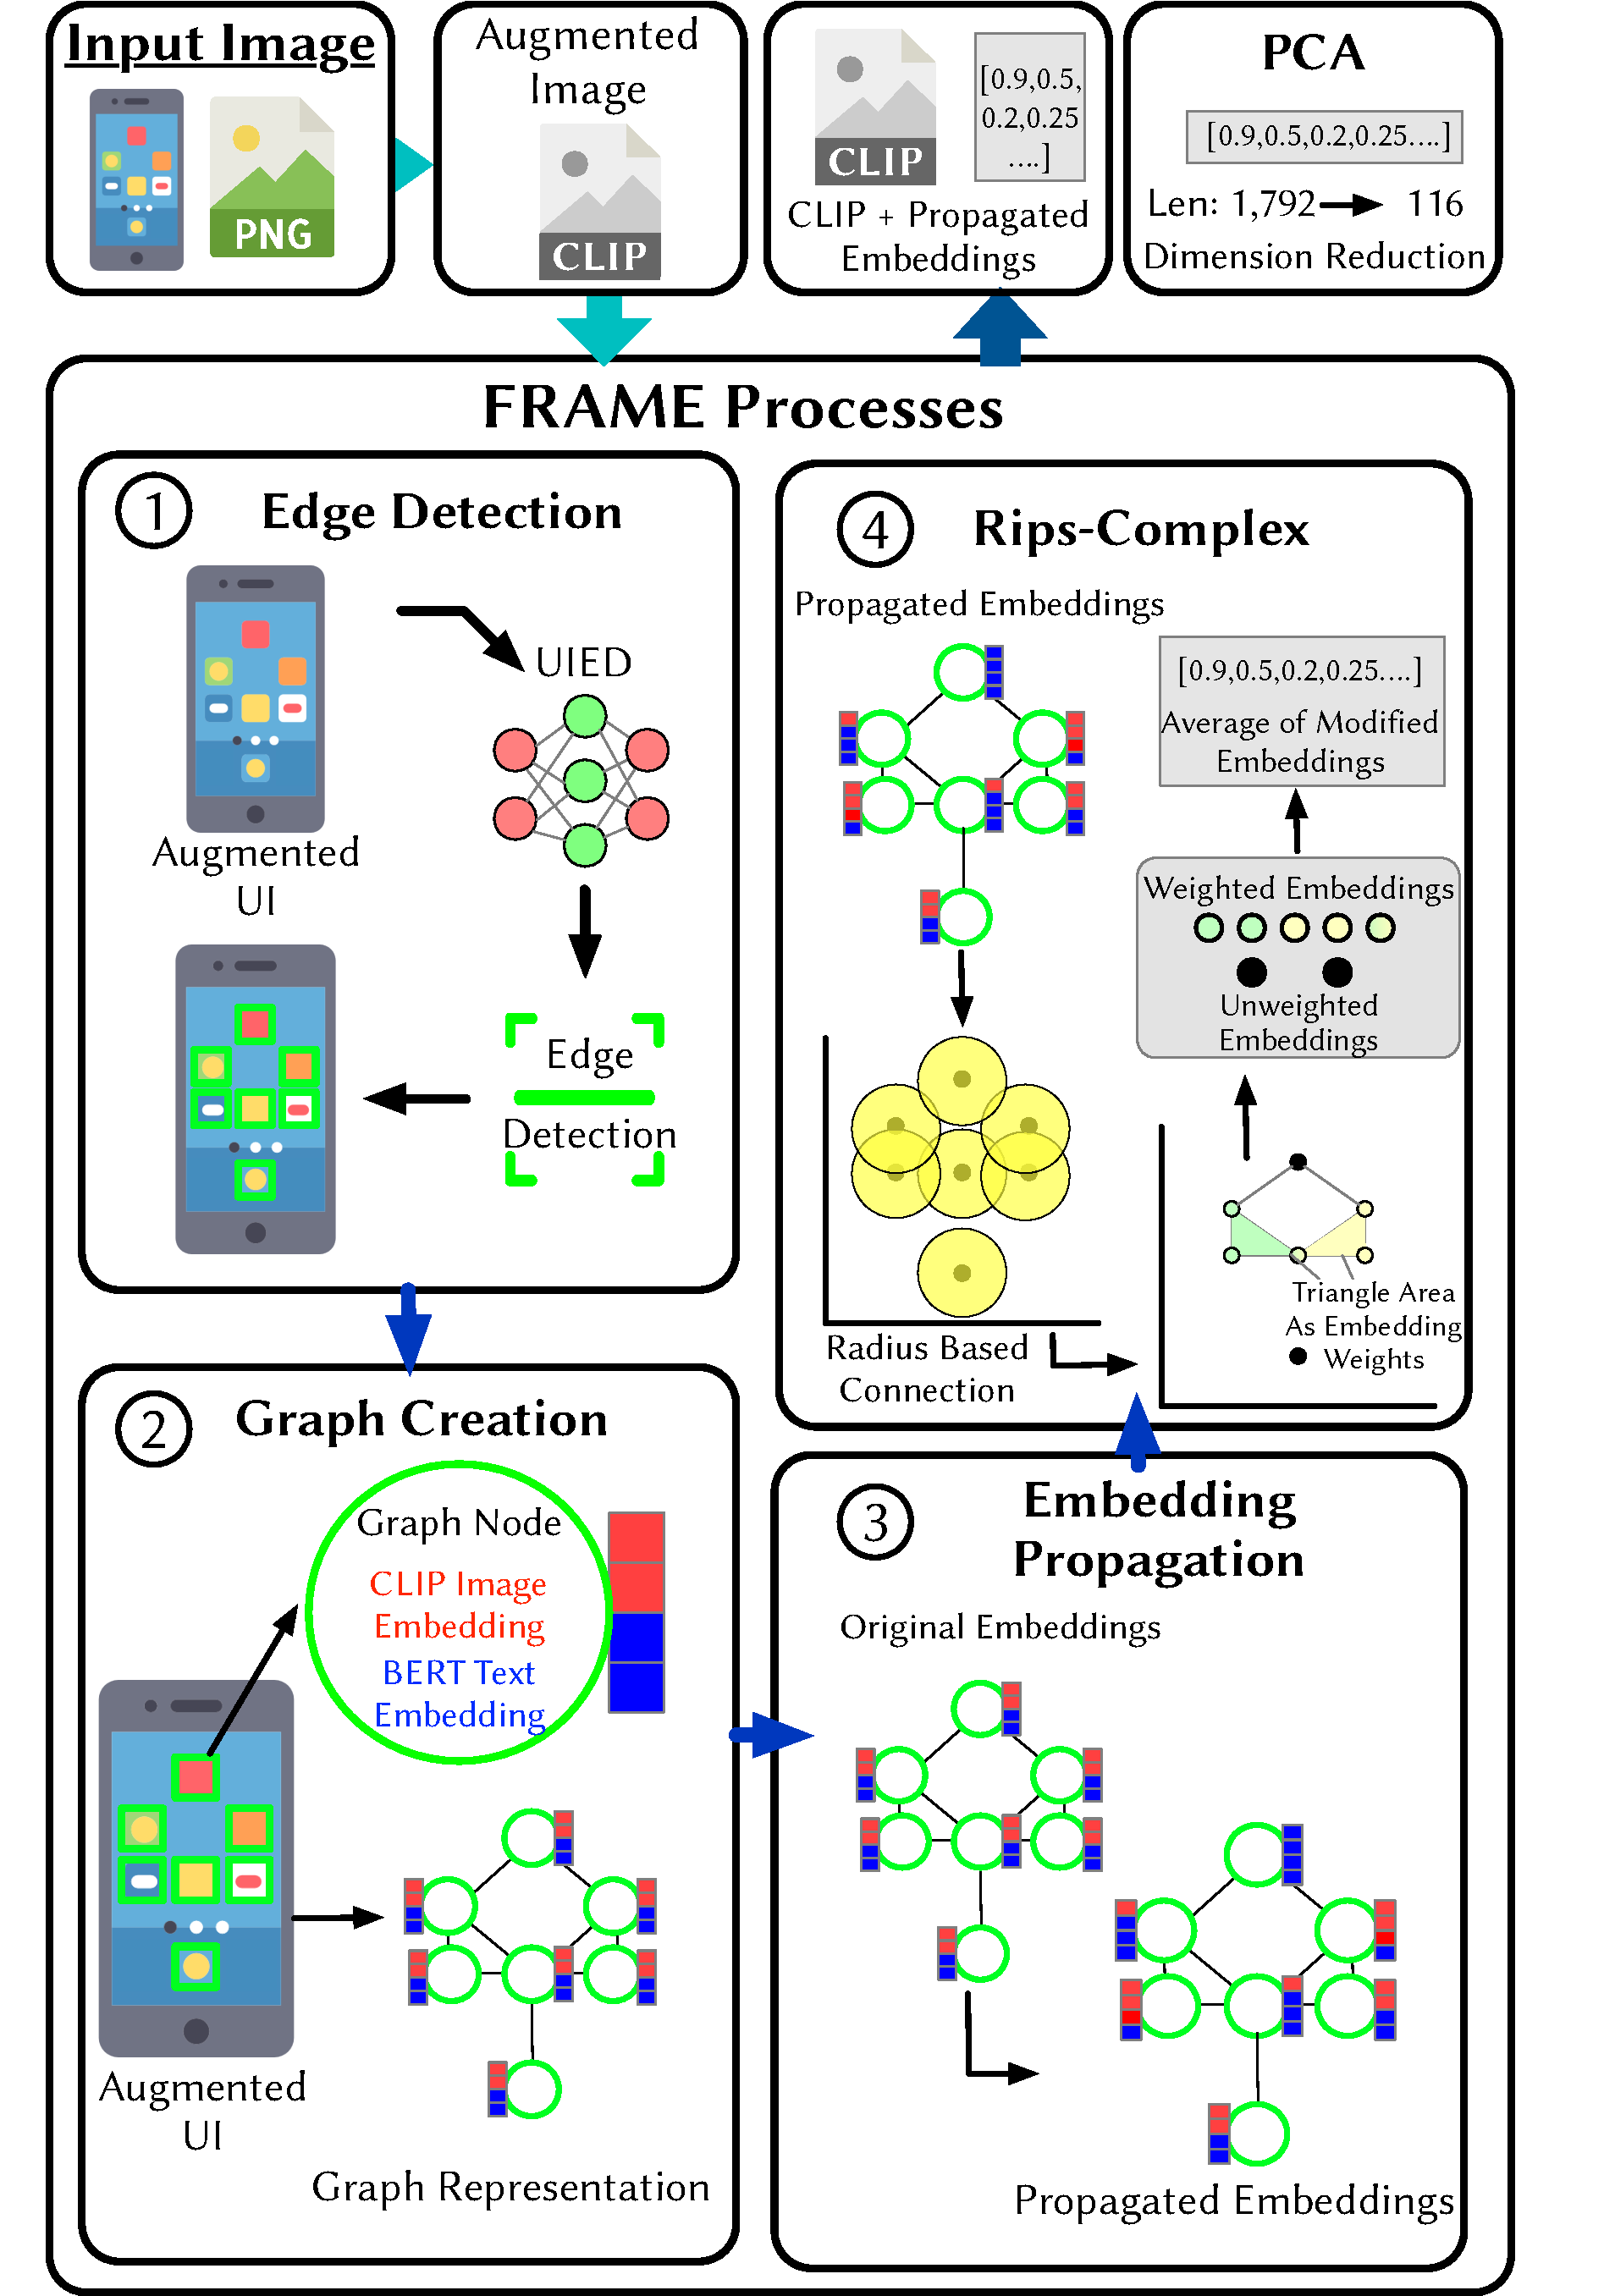
\includegraphics[width=0.6\textwidth]{imgs/FrameOverview.pdf}
    \caption{Overview of The FRAME Approach}
    \label{Overview}
\end{figure}

\FRAME is a structural-based approach to creating an image embedding that will aid in various screen similarity and retrieval tasks. To achieve this, \FRAME requires only the screenshot of a mobile app screen to generate the embedding. This is done as a way to maximize the use cases for \FRAME in any process that may require the embedding of a UI screen. \FRAME operates in five main stages to create the most structurally accurate representation of the screen. When a screen is given to \FRAME, it preprocesses the image using a series of image alteration techniques. We use the images and use edge detection to extract visual elements of the screen while retaining their positional information within the context of the screen. We create a graph-based representation of these elements and contextually weight the graph nodes based on their neighborhoods. Once that is done, \FRAME will take the new node embeddings and consolidate them using the Vietoris-Rips complex to consolidate the graph information into one embedding. The process of creating this embedding is visualized in Figure~\ref{Overview}. This embedding will be a structurally rich embedding which may aid in tasks requiring a numerical UI screen representation. 

\subsubsection{Pre Processing the Image}
Screens are designed to be visually pleasing and provide an intuitive placement of the elements such as icons and text boxes. In order for the embedding to abstract the elements on the screen and mitigate noise on the screen, \FRAME utilizes two screen preprocessing techniques. Noise on the screen can take many forms such as color palettes, customized icon designs, and different fonts. To mitigate these types of noise on the screen, \FRAME uses black-and-white as well as high contrast alterations to the screen. 
\subsubsubsec{black-and-white Modification}

\begin{figure}[h]
    \centering
    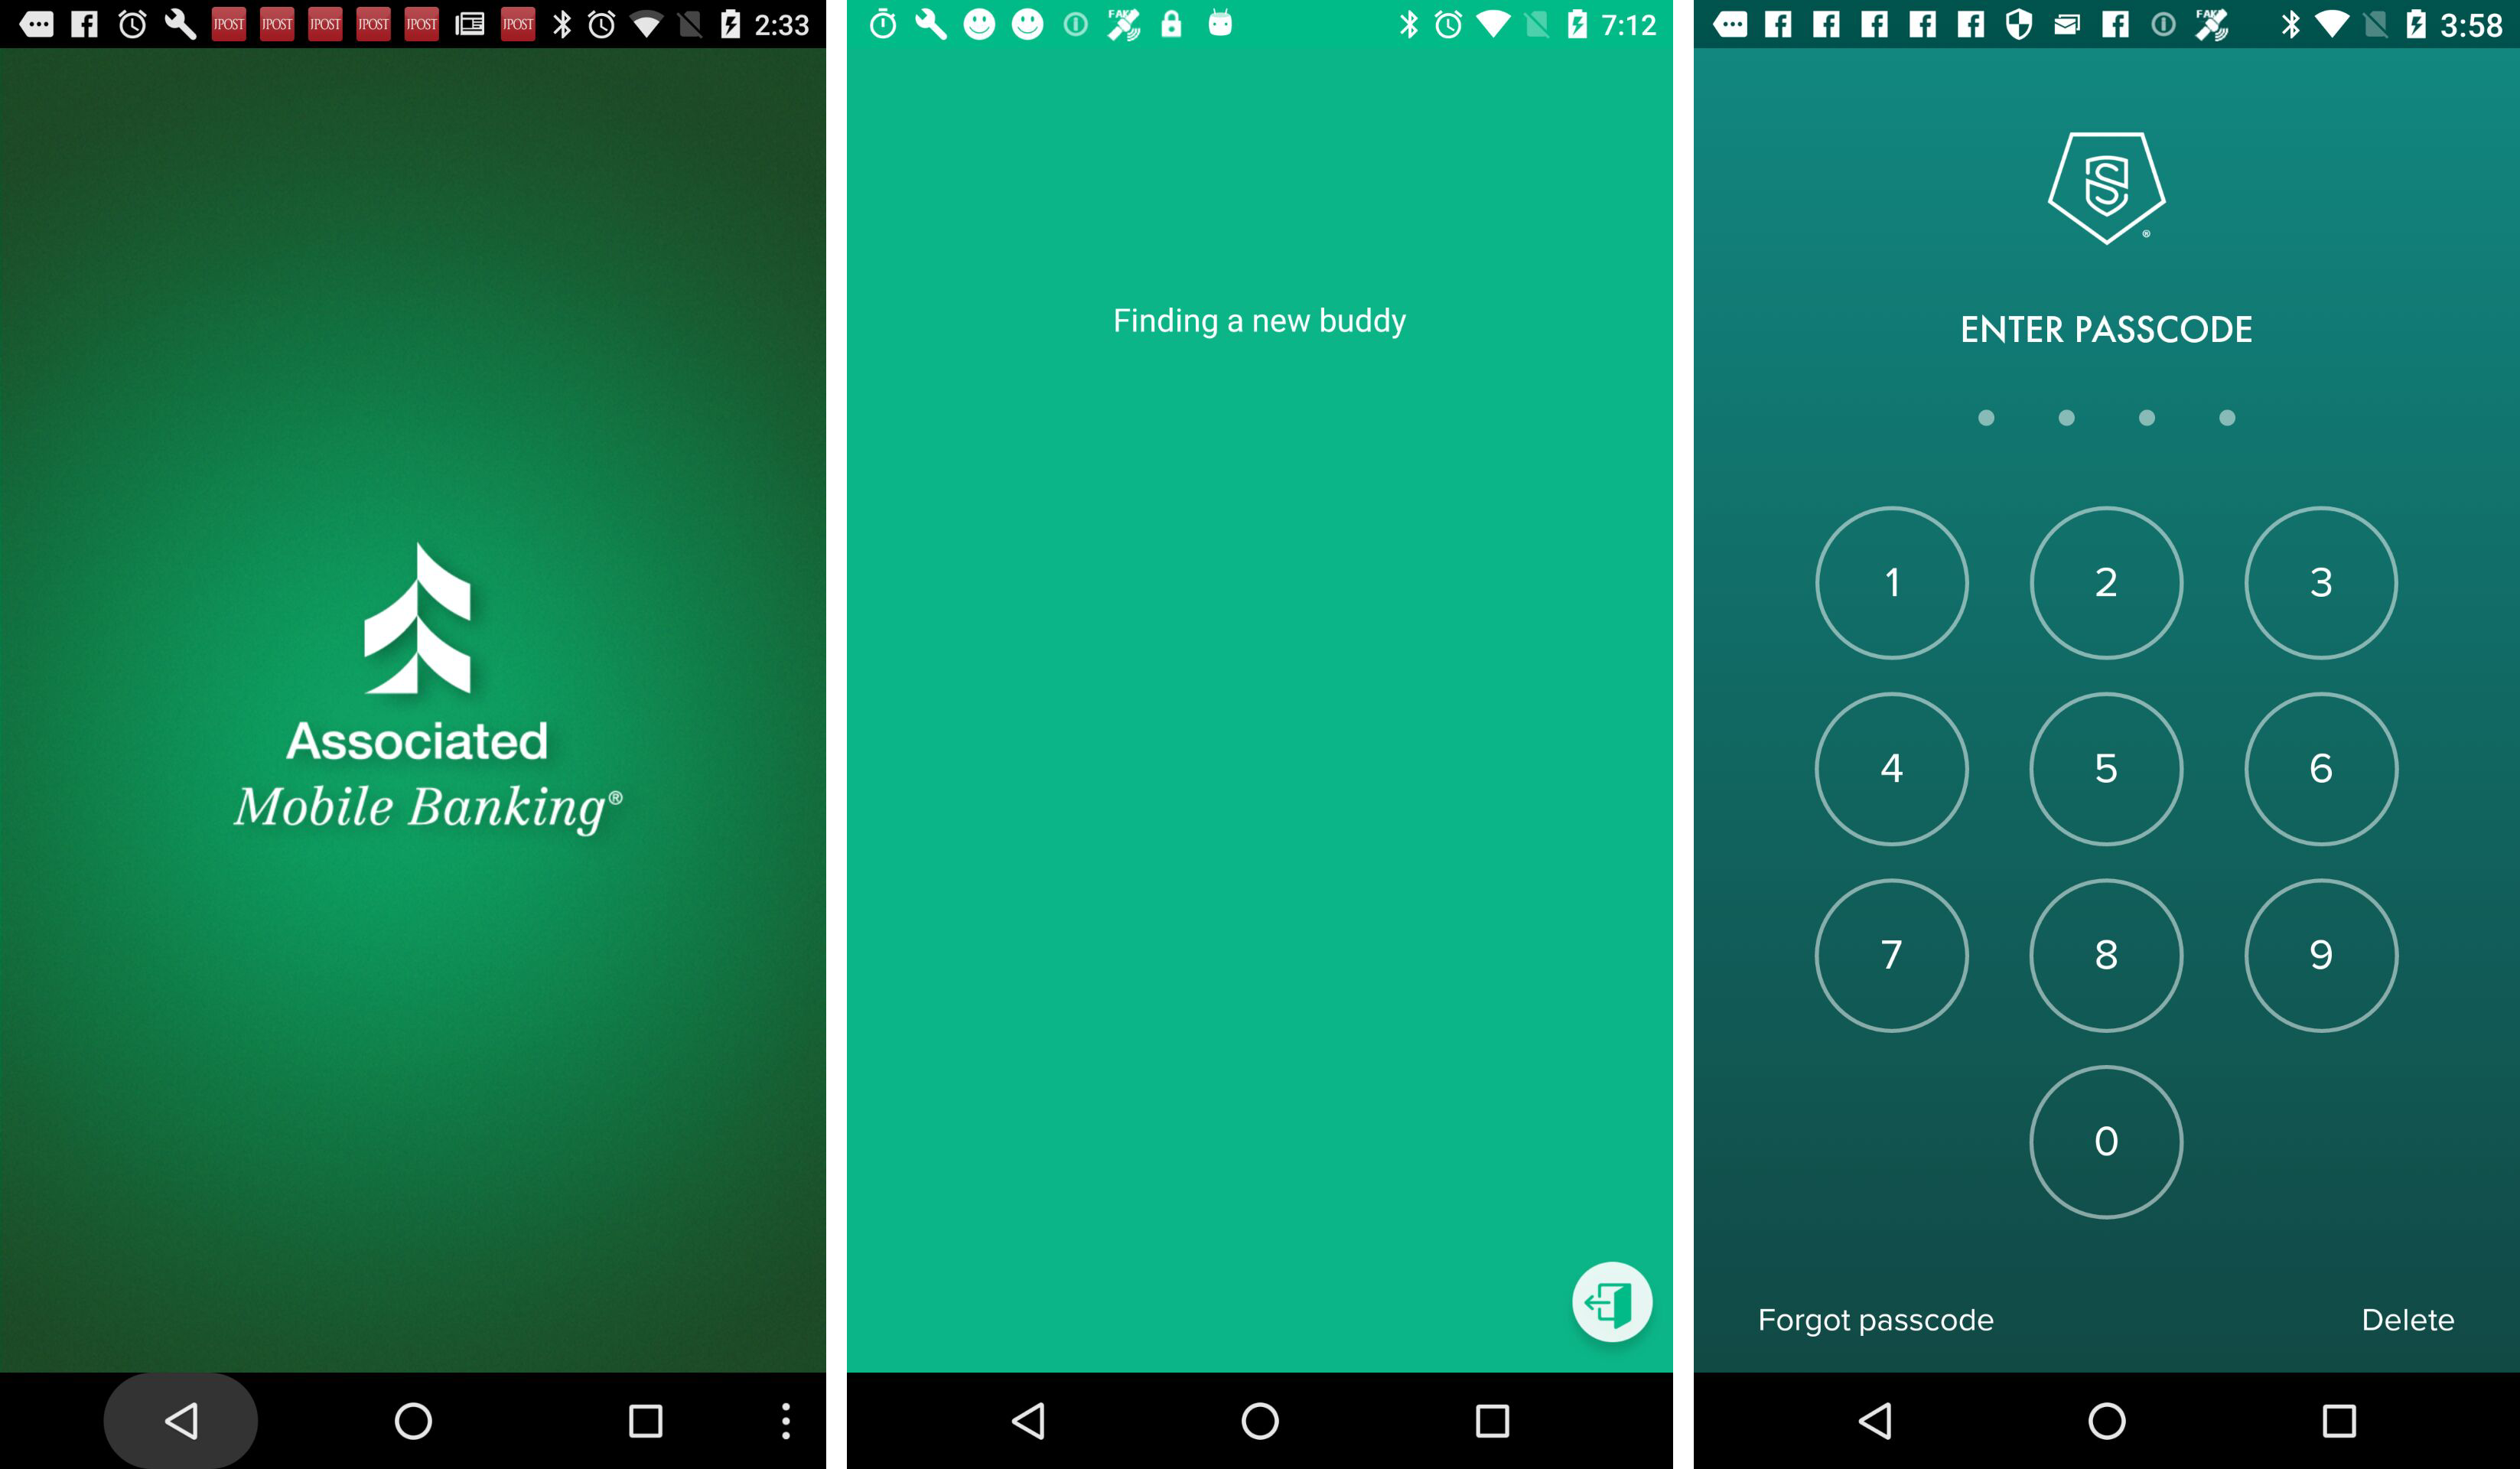
\includegraphics[width=0.55\textwidth]{imgs/3Clip.png}
    \caption{3 Similar Images using CLIP Embeddings}
    \label{3clip}
\end{figure}

\FRAME's goal is to provide skeletal-based similarity of screens rather than color. For example, Figure~\Ref{3clip} shows three images that were the most similar when using a CLIP embedding~\cite{clip}. The three screenshots have very similar color palettes and dominating colors upon visual inspection. On top of being similarly colored, these images do not share the same structural components and are three different types of screens. The leftmost screen is a Splash screen, the middle is a Search screen, and the rightmost screen is a password screen. Visual intuition suggests that these three screens provide different functions, but the CLIP embedding, which considers the colors of the screen, is unable to properly identify this discrepancy in the visual structure of the elements on the screen. To diminish the identified issues experienced by CLIP, we opt to remove color as a factor from consideration. We use the Pillow library's~\cite {pillow} grey scale conversion to convert the image to black-and-white first to ensure that no color is present in the extraction of the screen elements in the process of making the embedding. This can be seen in Figure~\ref{preprocessing} as the input image is made black-and-white. 


\begin{figure}[h]
    \centering
    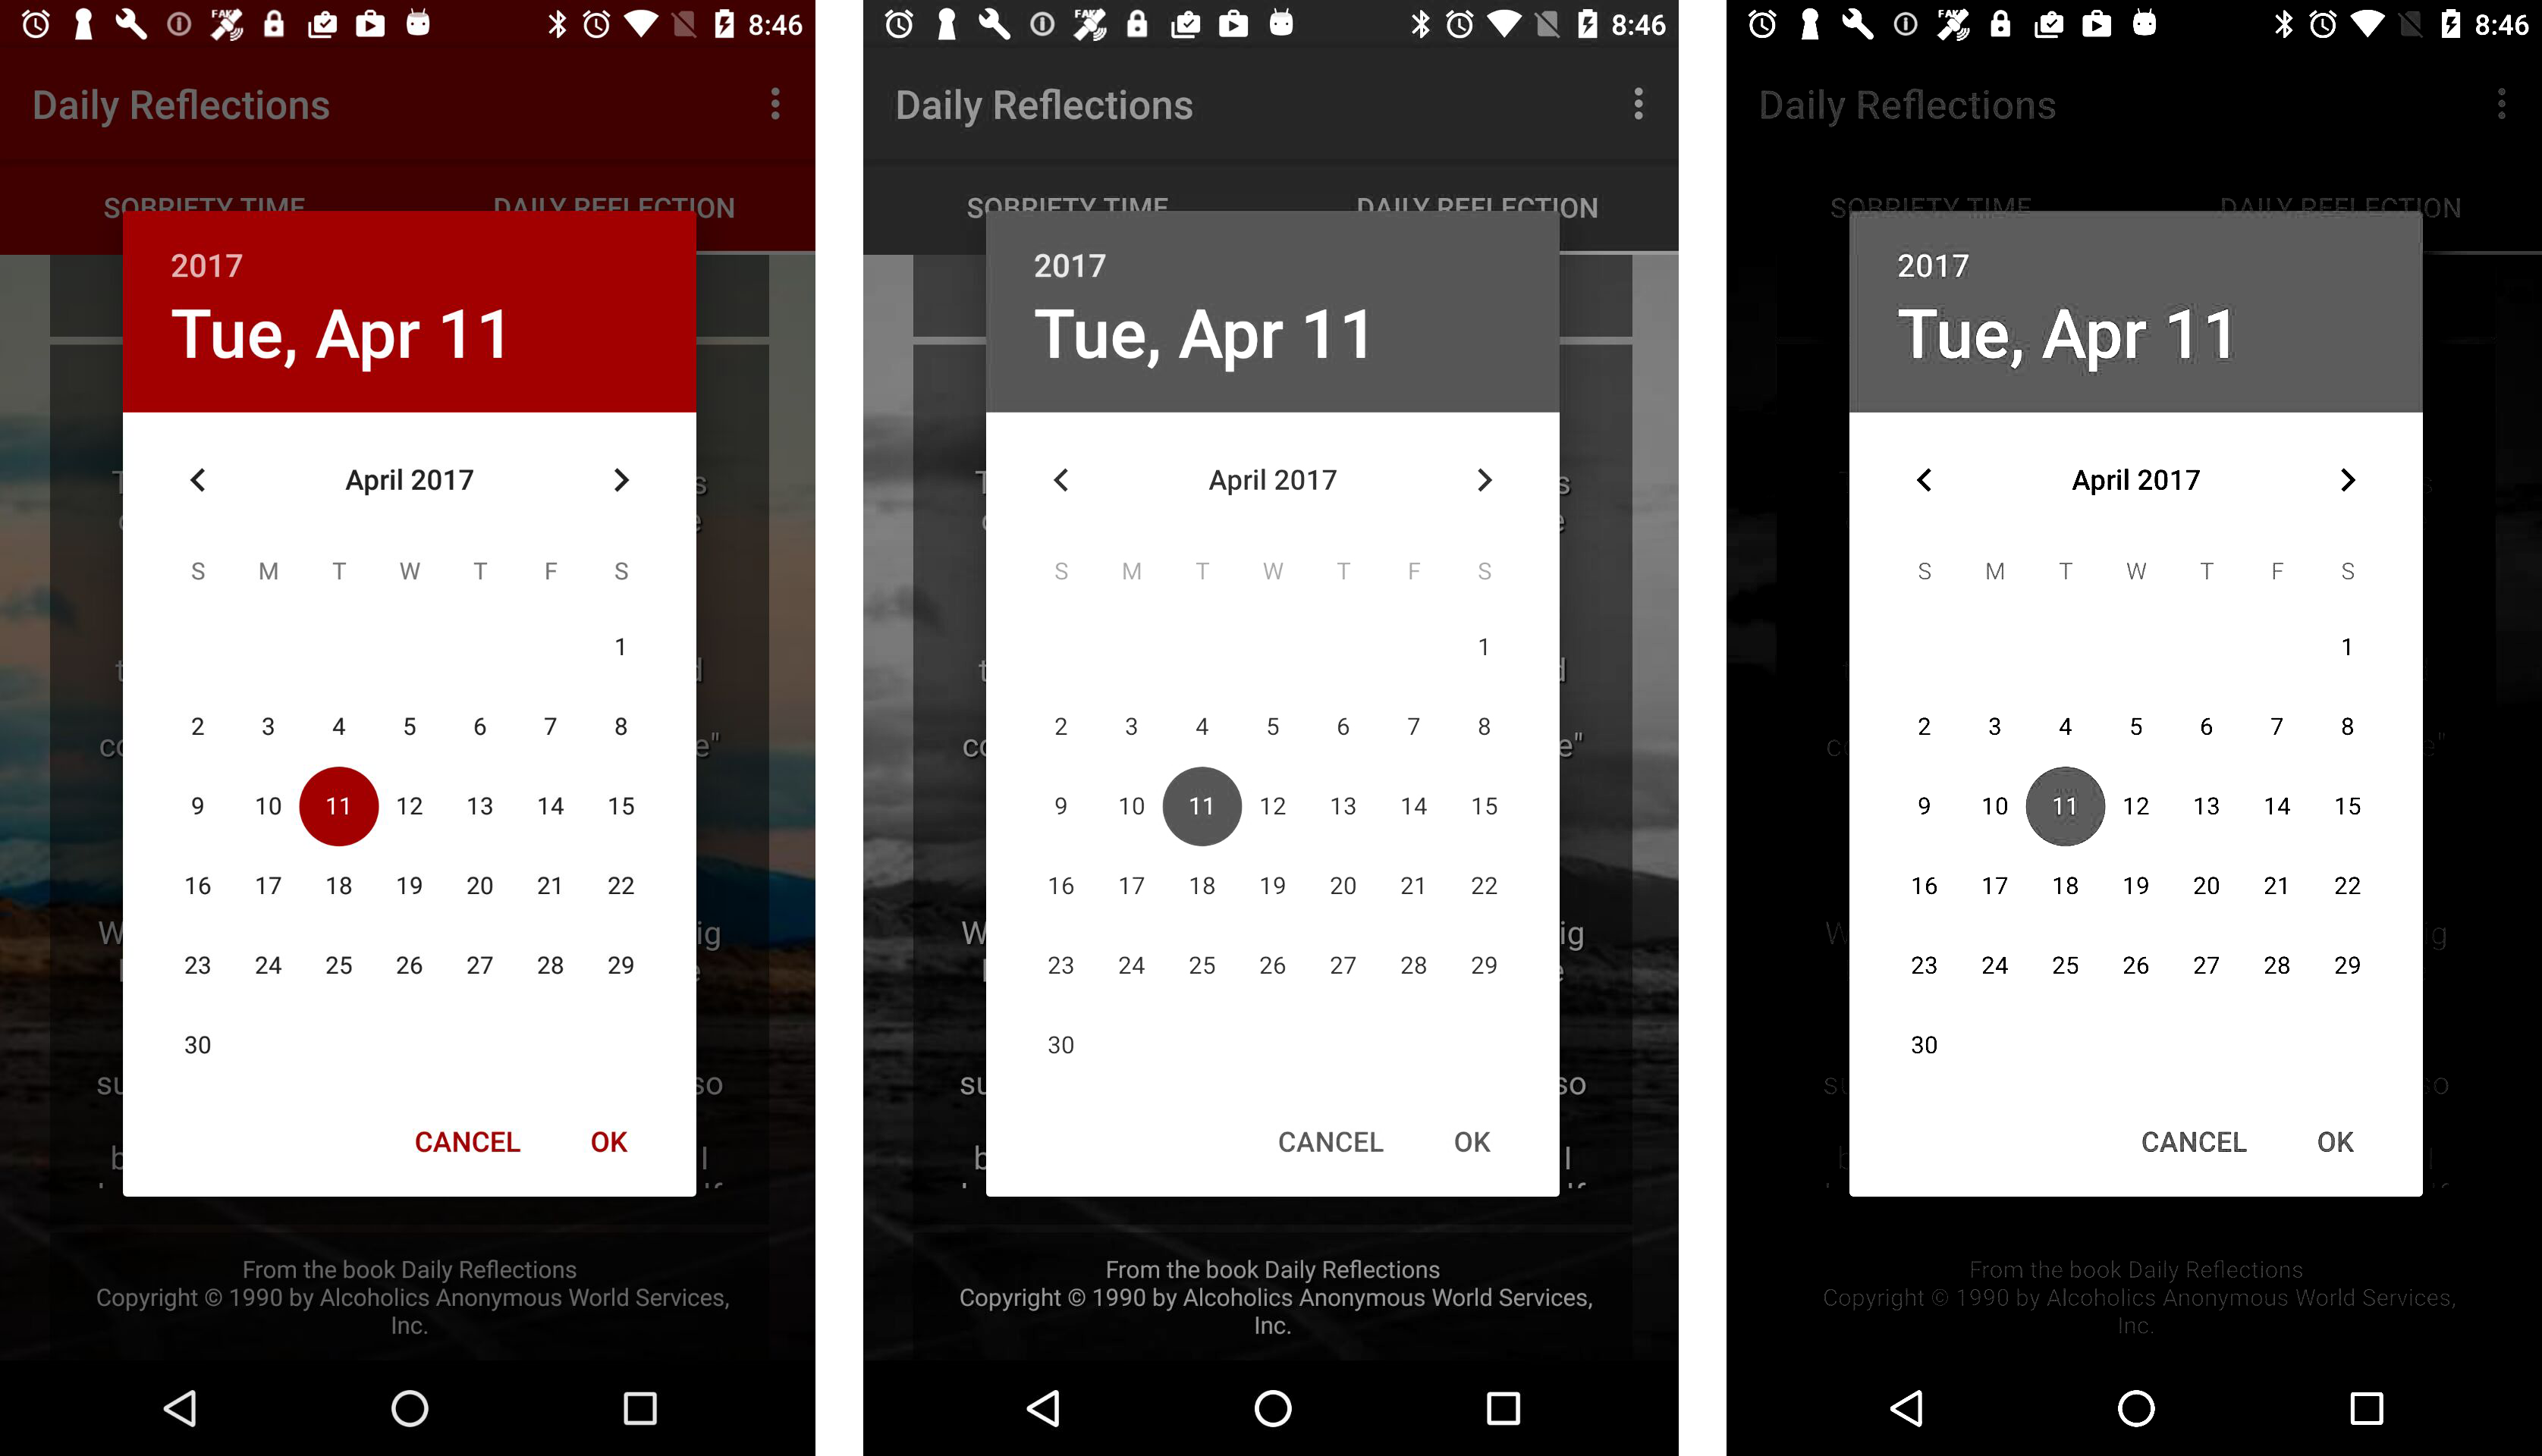
\includegraphics[width=0.55\textwidth]{imgs/PreProcessing.png}
    \caption{Preprocessing and augmenting the input image}
    \label{preprocessing}
\end{figure}

\subsubsubsec{High-Contrast} 


In addition to making each input screenshot black-and-white, we alter the images by increasing the contrast by 2X in the image. Contrast allows \FRAME to darken the dark pixels in the screen and brighten the brighter pixels in the screen. The resulting image has two main characteristics: (i) enhanced edge visibility; (ii) reduced noise influence. Enhanced edges are created because the colors on either side of the edge are modified, resulting in a more obvious and harsh edge. This aids the edge detection algorithm in finding accurate edges to accurately represent the screen's elements. Reduced noise is achieved by merging shades that are very close to each other, such as drop shadows, to create an abstract screen without many distractions for the edge detection algorithm. We use the Pillow library's~\cite{pillow} "ImageEnhance" sublibrary which has a contrast function to increase the contrast in the image. An example of this is shown in Figure~\ref{preprocessing}. We can see that the initial black-and-white image has less pronounced shades of greyscale colors and edges, while the high-contrast image has very clear boundaries between light and dark which can help facilitate edge detection. 


\subsubsection{Graph Creation}

To ingrain the visual structure of a UI screen, \FRAME utilizes a graph to plot nodes in similar areas as they appear on the screen. These nodes are created by the individual elements of the screen and their positional information. This positional information combined with elemental embedding information provides for a rich node within the graph to define relations between elements within the graph neighborhoods. There are three stages to developing a graph for each screen. 


\subsubsubsec{Edge Detection}

 \FRAME's goal is to create an embedding with the same intuitive structural pattern humans notice in their UIs. This is motivated by the examples of screens shown in Figure ~\ref{3clip}. We identify that passcode screens traditionally have the keypad in the center and that splash screens traditionally have the logo of the app in the center while surrounded by color. Being able to extract the icons and elements of the screen that suggest these patterns is a key element in creating an embedding that is capable of identifying these patterns. The edge detection approach used is an open-source edge detection model called UIED ~\cite{UIED}. UIED is specialized to work with UI Screens and provides high-quality element detection. This approach is further aided by the preprocessed image. \FRAME takes the edge detector's output and crops out each image. \FRAME only considers images larger than 48x48px since that is the standard for minimum accessible icons on an Android screen as per Google's Accessibility Guidelines ~\cite{GoogleAccess}. UIED gives the bounding box for each element as well, which can be used to find the centralized (x,y) point where the element is located on the screen. This is the positional information for each extracted element on the screen. 

\subsubsubsec{Graph Creation}


Icons on the screen have contextual information to offer to a screen. For example, a magnifying glass icon can indicate search, or a gear wheel icon may suggest settings. In addition to the positional information obtained through UIED, \FRAME takes into account the visual and textual aspects of each icon on the screen. To do this, we take the cropped icon provided by UIED and create 2 embeddings from it, an image embedding using CLIP, and a text embedding using BERT~\cite{BERT}.

\begin{figure}[h]
    \centering
    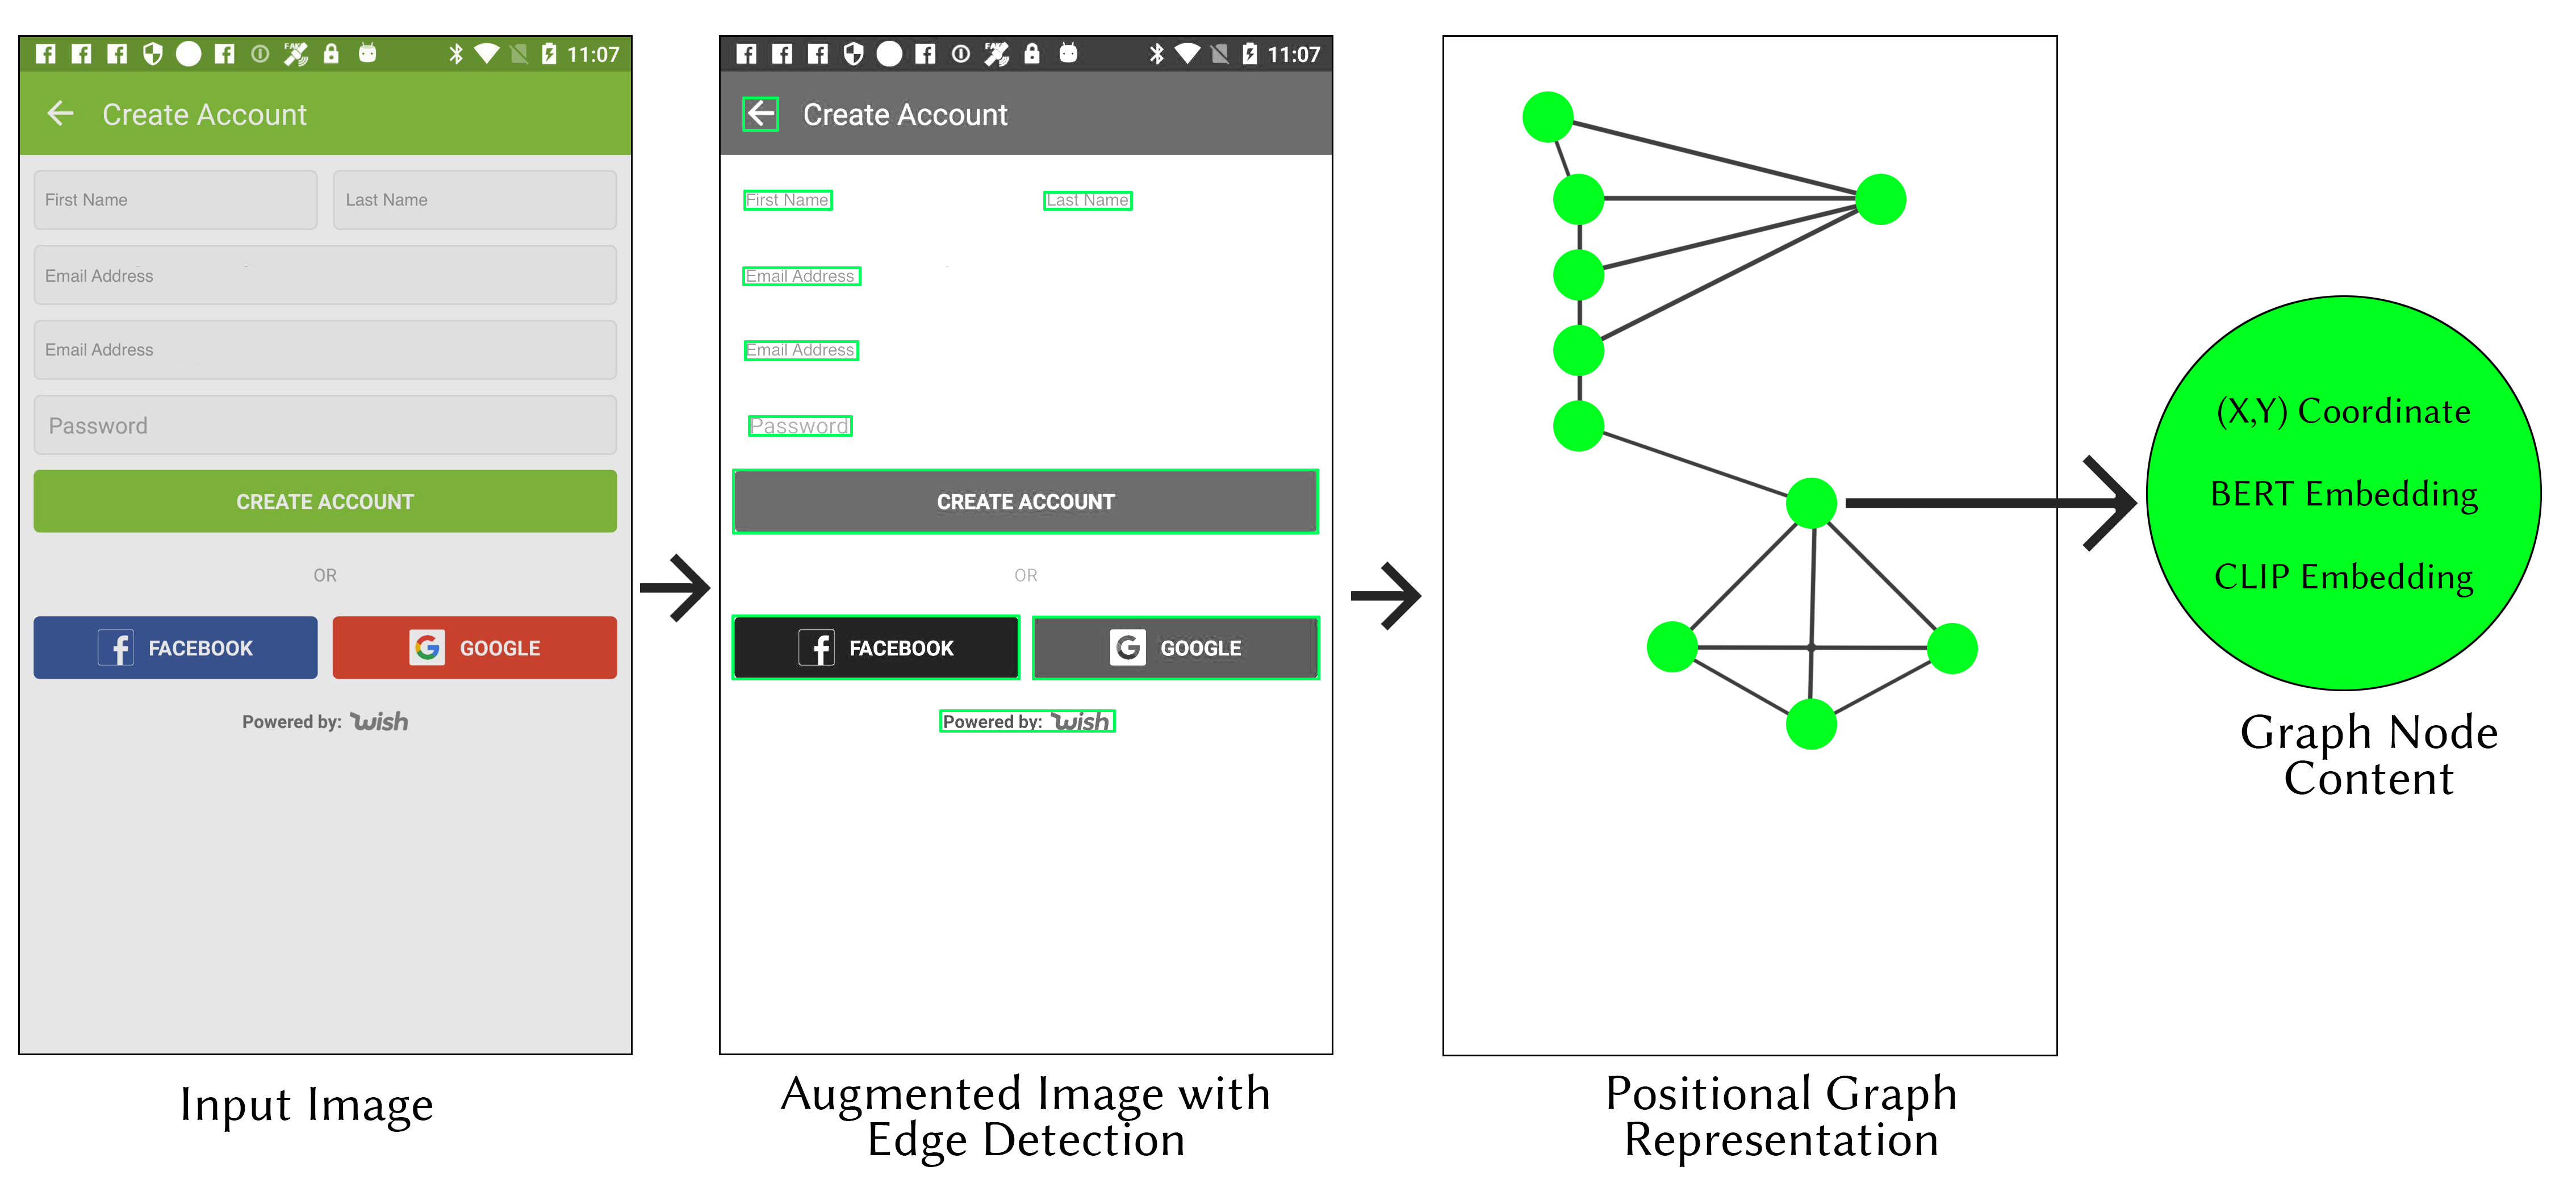
\includegraphics[width=0.7\textwidth]{imgs/graphCreation.png}
    \caption{Process of creating the graph}
    \label{graphCreation}
\end{figure}


\underline{\textit{Image Embedding:}} Though CLIP may not capture structure that well, CLIP is excellent at identifying stylistically similar screens as shown in Figure~\ref{3clip}. We use this property of CLIP to create embeddings for each icon on the screen. We create the icon embedding and add it to the node in the graph that represents the element on the screen. As shown in Figure~\ref{graphCreation}, each node has a visual representation of the icon that is cropped out of the screen.
 
\underline{\textit{Text Embedding:}} BERT is currently the most advanced text embedding available and we utilized it to create textual embeddings for each icon. Icons may have text in them, for example, the Facebook icon has the letter "F" and the word "Facebook" under the logo. We can leverage this text to add more depth to each node within the graph. We use PyTesseract to extract text from each cropped icon. We take the extracted text and clean it using regex functions to make it clean text. \FRAME takes the extracted, cleaned text and creates the BERT embedding to add to the graph node. As shown in Figure~\ref{graphCreation}, each node has a textual representation of the icon that is cropped out of the screen. In the case there is no text, a single space character is used as default. 

With the inclusion of the image and text embeddings within each node as well as the (x,y) positional coordinate for each icon, the nodes in the graph are filled with niche data that is localized to each icon. This gives each node a unique set of features that sets it apart from other nodes within the graph and its neighborhoods. We can utilize this diversity of node information to create a graph that can map relations between nodes based on their embedding data. 

\underline{\textit{Graph Edges:}} Once nodes for the graph are created, \FRAME takes into account the positional distance between the nodes in the graph and connects nodes that are within a certain distance to each other on the screen. The graph connects nodes that are a maximum of 300 pixels in distance from each other when using Manhattan distance. On average, the distance between icons on the screens is 300 pixels as observed by the authors. Therefore, we elected to use the average distance as the threshold for edge connection to ensure that the resulting graph does not lack edges or appear overly complete. This approach allows for the formation of distinct neighborhood clusters within the graph. The graph is built with nodes that have position coordinates, BERT embedding, and CLIP embedding and are connected via edges to form neighborhoods. This is shown in Figure~\ref{graphCreation}. \FRAME aims to find patterns between close elements, so having the connections be a maximum distance of 300 pixels allowed the graph to have distinct neighborhoods of nodes on different parts of the screen. This helps localize icon clusters and elements on the screen that may closely be related to each other. 



\subsubsection{Graph Embedding Propagation}
Unlike ordinary images, GUI screens exhibit a more structural nature, with closer relationships existing between adjacent components. Therefore, we augment the image/text embedding of each component by its neighbor component embeddings based on the constructed structural graph. This is inspired by a recent work for code embedding augmentation by leveraging the program dependence (i.e. structural) graph constructed for a software system  \cite{yanfu2024athena}. Specifically, our embedding propagation strategy is derived from the first-order approximation of localized spectral filters on graphs \cite{kipf2016semi, defferrard2016convolutional}, which can be represented as follows: 

\begin{equation} 
    S' = (I_N + w D ^ {-\frac{1}{2}} A  D ^ {-\frac{1}{2}}) S. 
\end{equation} 

$S \in \mathbb{R}^{N \times M}$ represents the matrix of all the image/text embeddings of nodes from $G$ and $S'$ represents the updated matrix by incorporating the information from the neighbor nodes. $M$ denotes the dimension of each image/text embedding (i.e. $768$) and $N$ denotes the number of nodes in the graph. $A$ is the adjacency matrix of $G$ without self-connections and $D$ is the degree matrix of $A$ so that the adjacency matrix is normalized by $D$ with respect to both the row and the column. $w$ is a constant to balance the information from the original node/component with structural information from the neighbor nodes/components. By leveraging the embedding propagation strategy, the image/text embedding for each component will encompass more structural information from its adjacent components, which is expected to further enhance GUI screen understanding. A visual representation of this process is shown in Figure \ref{Overview}-3.  


\subsubsection{Rips-Complex}

We realize the propagated UI embeddings as a set of points in Euclidean space to capture information regarding the topological relationship of the embedded data. This is achieved by triangulating the points to create a structure known as a simplicial complex as shown in Figure~\ref{fig:simplex}. 

\begin{figure}[h]
    \centering
    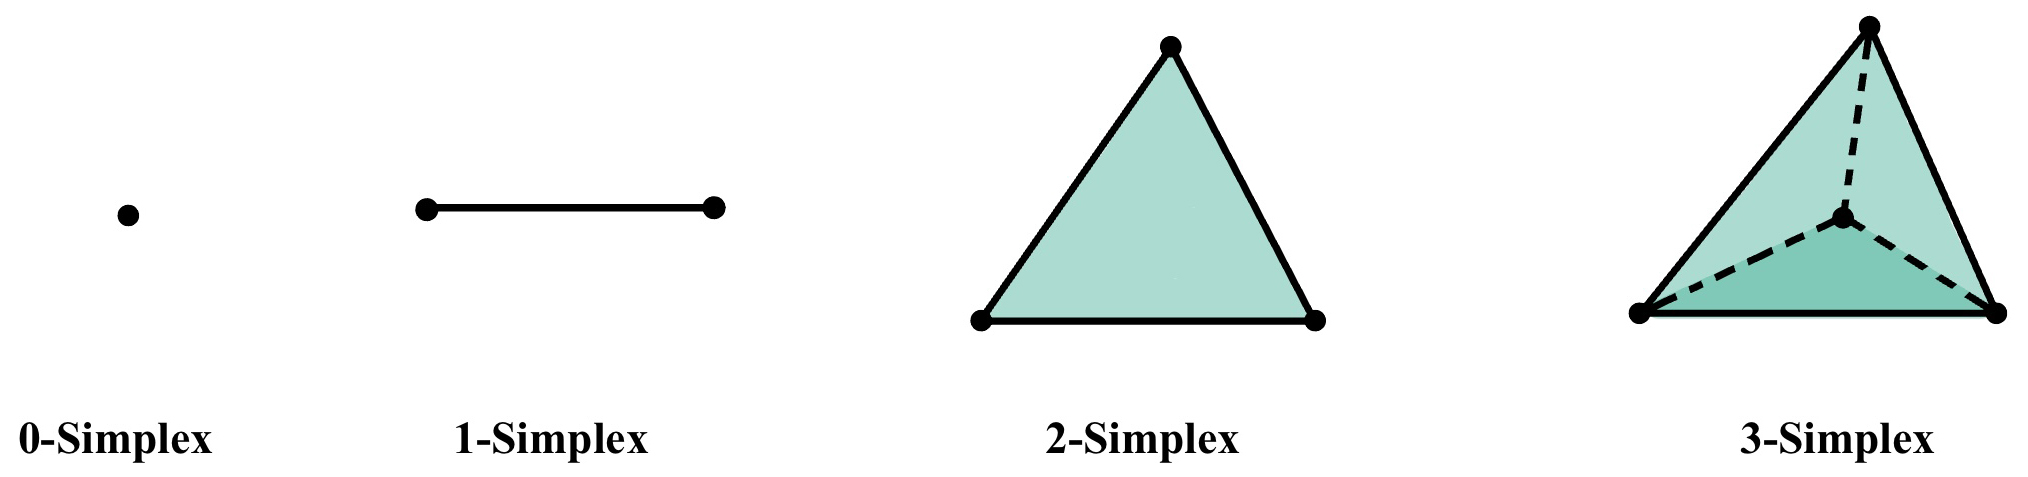
\includegraphics[width=0.6\textwidth]{imgs/simplexMod.jpg}
    \caption{Visualization of low dimensional simplicies}
    \label{fig:simplex}
\end{figure}

A simplicial complex is created by plotting the propagated embeddings on a graph in Euclidian space. We use our embeddings to create an object known as the Vietoris-Rips complex (often called the Rips complex) using GUHDI \cite{gudhi:RipsComplex}. Given a parameter $\epsilon>0$, the Rips complex of embeddings $\mathcal{X}$ is made into a simplicial complex that captures the spatial and topological relationships between the points in space using the following definition: 

\begin{definition}
Given a set of embeddings $\mathcal{X} = \{x_1, x_2, \hdots, x_k\} \subset \mathbb{R}^{n}$ and an $\epsilon>0$, a $k$-simplex $\sigma = [x_{i_1}, x_{i_2}, \hdots x_{i_k}]$ is in the Vietoris-Rips Complex $\textit{Rips}_{\epsilon}(\mathcal{X})$ if and only if:
\[ \mathbb{B}_{\epsilon}(x_{i_j}) \cap \mathbb{B}_{\epsilon}(x_{i_{j'}}) \neq \emptyset \]
where $\mathbb{B}_{\epsilon}(x_{i_j})$ is an open ball at $x_{i_j}$.
\end{definition}

\begin{figure}[h]
    \centering
    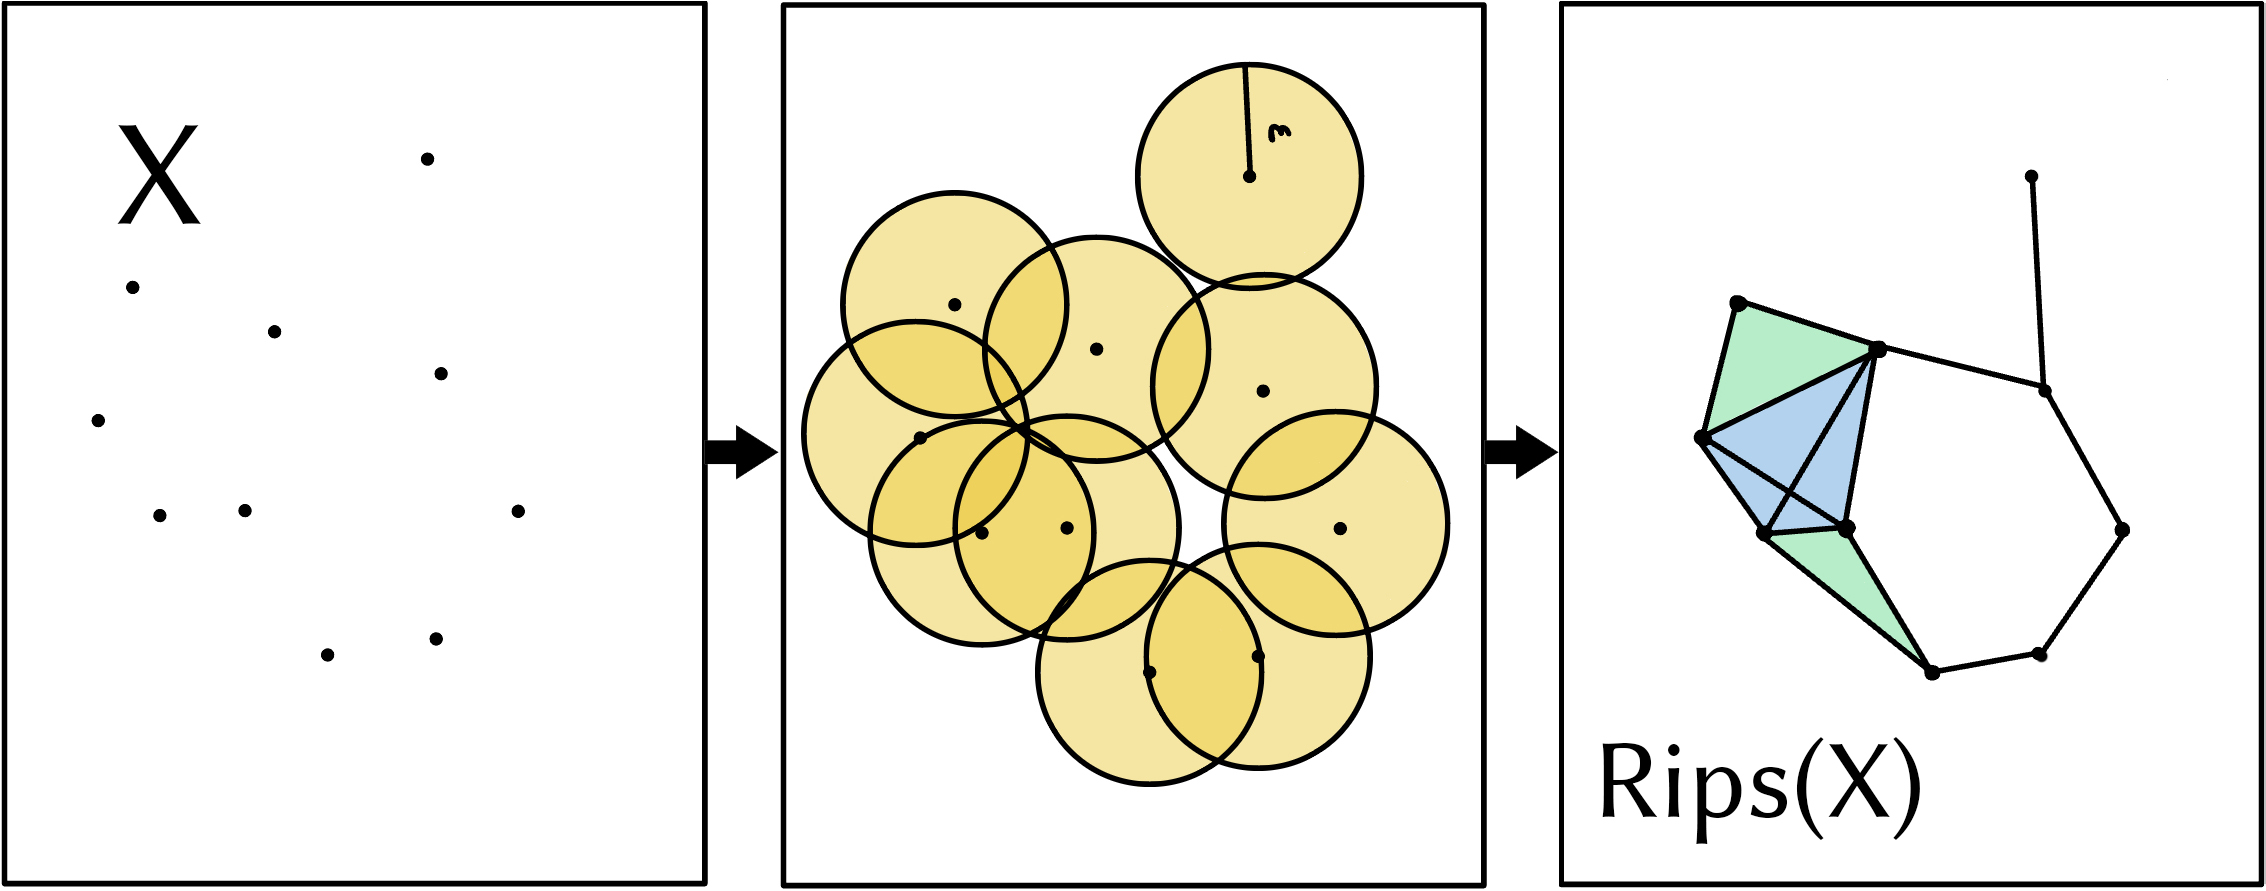
\includegraphics[width=0.6\textwidth]{imgs/RipsMod.jpg}
    \caption{Process of creating the Rips Complex using a set of embeddings}
    \label{fig:Rips}
\end{figure}

$\epsilon>0$ is the radius of the open ball used to determine edge connections within the embedding space. For small parameters of $\epsilon$, the open balls are too small to intersect and result in a complex with only the original embeddings. On the opposite end, if $\epsilon$ is too large, every feature in the input image is related to every other feature. We selected $\epsilon$ by performing a parameter study from $0.1-1$ in increments of $0.05$. Our ideal value of $\epsilon$ captures the average 100-200 features present in an input image. This was chosen to be $\epsilon=0.5$, as it resulted in an average of 100-200 $2$-simplicies generated in the Rips complex. The process of overlapping open balls and simplex creation is shown in Figure \ref{fig:Rips}. 

By employing the Rips complex on the propagated UI embeddings we are topologically capturing the relationship between an object in an image with all other objects in the image as shown in Figure \ref{fig:Rips}. Once the simplex is created, we consider the embeddings that make $2$-simplicies (2D triangles) and use the area of the resulting simplex as a weight for the involved embeddings. The area of a given 2-simplex can be calculated using Heron's formula \cite{weisstein2003heron}:
\begin{equation}
    \text{Area} = \sqrt{S(S-A)(S-B)(S-C)}
\end{equation}
\noindent where $S$ is the semi-perimeter of the 2-simplex and $A,B,$ and $C$ are the lengths of its three edges. The area is then used to weigh the involved embeddings.

We employ the Area-based Triangulated Embedding method (ATE), proposed by Krishna Vajjala et al. \cite{vajjala2024vietoris}, for the weighted average of the embeddings. This creates a weighted relation between embeddings that are close to each other, resulting in a weighted preservation of information between those three embeddings. We do this until we have a set of weighted and unweighted embeddings. We then average these embeddings together into one final embedding. A visual representation of this process is shown in Figure \ref{Overview}-4. 

\subsubsection{Final Embedding}

\FRAME embeddings reinforce existing embeddings by adding structural understanding to an image. The process of creating a distance-similar graph, propagating the embeddings within it, and consolidating them using the area-based triangulation creates a structure-encoded set of embeddings. This set of embeddings can then be added to the initial pre-processed CLIP image embedding. This results in an embedding that has the pre-processed version of the CLIP embedding along with the propagates structural relations between the icons on the screen which are a CLIP and BERT embedding combined. The resulting embedding is noisy and large with a size of 1,792 dimensions. To combat this, \FRAME uses PCA \cite{PCA}, a dimension reduction technique to reduce noise in high-dimension vectors. PCA takes a list of vectors and identifies the directions (principal components) where the data varies the most. By projecting the original data onto these principal components, PCA effectively reduces the dimensionality of the dataset while preserving as much of the original information as possible through linear transformations. We use Google's Scikit-Learn's~\cite{sklearn} PCA which takes as input a series of vectors and the desired size of the vector. We considered the training data vectors from both of our datasets and ran a hyperparameter study to determine the best size for the resulting vector. The resulting vector size is reduced from 1,792 down to 116. To ensure that new embeddings result in size 116 without re-running PCA on the dataset, we use PCA's transformation matrix and do a dot product with the initial noisy vector and the transformation matrix to obtain the 116 size representation of the new embedding. 

\subsection{Evaluation Methodology}

\setlist[questions,1]{label=RQ\arabic*.,ref=RQ\arabic*}
\setlist[questions,2]{label=(\alph*),ref=\thequestionsi(\alph*)}
In this section, we describe the procedure we used to evaluate \FRAME. To achieve our study goals, we formulated the following
four research questions:

\begin{itemize}
	\item{\textbf{RQ$_1$} \textit{How does \FRAME perform against other baselines in screen retrieval tasks}}
	\item{\textbf{RQ$_2$} \textit{How does \FRAME perform on various types screens against the best baseline?}}
        \item{\textbf{RQ$_3$} \textit{How important is the structural embedding propagation between graphs in order enhance the embedding ?}}
        \item{\textbf{RQ$_4$} \textit{How well does \FRAME leverage its ability to abstract the screen and disregard styling?}}
        
\end{itemize}

\subsubsection{{\FRAME Evaluation Database}}
\FRAME is designed to understand structural aspects of the screen. Screen retrieval tasks are a suitable benchmark for \FRAME since the embedding will need to effectively identify other screens with similar visual layouts regardless of colors and text differences. This means that the evaluation for \FRAME has to focus on screen similarity and retrieval tasks that require \FRAME to find screens labeled of the same category. 

We evaluate \FRAME with two different databases, Avgust~\cite{Avgust} and Aurora~\cite{khan24}. 

\subsubsubsec{Aurora Dataset} 
While creating the Aurora tool~\cite{khan24}, authors created a labeled version of the RICO dataset with a small subset of the images. The RICO dataset is a set of 66,000 unique UI screenshots~\cite{Rico}. However, this dataset is just a set of screens and they are not labeled. The labeled Aurora dataset was made by selecting a 1\% subset of RICO UI images randomly. Then they performed an unlabeled clustering of the images based on their visual properties. They used k-means clustering and clustered them into groups. The authors manually examined the clusters and collectively agreed to label them into 21 distinct categories. This process resulted in a high-quality dataset to evaluate screen retrieval and search algorithms. This dataset has 21 distinct categories and 1370 screens. It is a sparse dataset and can test \FRAME's ability to find similar screens in a dataset with lots of variability. We divide this dataset using a 90 to 10 train-test split for testing. The resulting evaluation dataset is 1233 train images and 137 test images. 

\subsubsubsec{Avgust Dataset}
The Avgust dataset is another subset of the RICO dataset. This dataset is obtained from the Avgust paper by Zhao et al.~\cite{Zhao:FSE22}. It has 25 labels with 2475 total screens. This dataset was manually labeled by 4 authors who mutually agreed on each screen's category. This is a dense daset with above 130 screens per category on average. For testing, we divide this dataset using a 90 to 10 train-test split. The resulting evaluation dataset is 2219 train images and 256 test images. 


\subsubsection{\textbf{RQ$_1$} \textit{How does \FRAME perform against other baselines in screen retrieval tasks?}}
\label{sec:eval_metrics}
To evaluate \FRAME, we use two common information retrieval metrics to test its ability to find similar screens properly; we use Hits@k and Mean Reciprocal Rank (MRR). 

\subsubsubsec{Hits@k}

Hits@K is a metric that evaluates the effectiveness of information retrieval systems by measuring how many relevant items appear within the top K results. It assesses the tool's ability to provide relevant content within a specified top K number of ranked items. For example, Hits@10 would quantify the percentage of relevant items found within the top 10 results. This metric is beneficial for evaluating search algorithms and retrieval tasks, as it prioritizes the most relevant results users will likely encounter. 

\begin{equation}
\text{Hits@}k = \frac{\text{Number of relevant items in top }k\text{ results}}{k}
\end{equation}

We perform Hits@k with three different K values, 1, 5, and 10. When using Hits@K, a higher K value can make for a more lenient evaluation, having smaller numbers results in a rigid evaluation of the embedding that can provide true insight into its performance. In our assessment of \FRAME, we input a test image labeled with a specific category, then examine the top K images most similar to the test image to determine how many of them share the same label. This gives us an accurate representation of how \FRAME is able to find similarly structured screens. We perform this evaluation on both the Aurora and the Avgust datasets to test its ability to find similar screens in sparse and dense datasets. 

\subsubsubsec{Mean Reciprocal Rank (MRR)}

Mean Reciprocal Rank (MRR) is a metric commonly used in information retrieval and ranking tasks. It calculates the average of the reciprocals of the ranks at which the relevant items are retrieved. For instance, if a relevant item is found at rank 3, its reciprocal would be \( \frac{1}{3} \). If another relevant item is found at rank 5, its reciprocal would be \( \frac{1}{5} \). The MRR is then calculated as the average of these reciprocals. 

\begin{equation}
\text{MRR} = \frac{1}{N} \sum_{i=1}^{N} \frac{1}{rank_i}
\end{equation}

MRR provides a single numerical value that summarizes the performance of the system across multiple queries, making it useful for evaluating and comparing different ranking algorithms or search models. In our assessment of \FRAME, we input a test image labeled with a specific category, then examine the list of images most similar to the test image to find the first image with the same label as the test image. This evaluation provides insight into how well \FRAME identifies similar images as higher in the list of similar images. We perform this evaluation on both the Aurora and the Avgust datasets to test its ability to find similar screens in sparse and dense datasets. 

It is important to understand how well \FRAME performs on its own, but having it perform the same tasks as other, common, baselines provides an insight into how well \FRAME is able to perform in information retrieval tasks. We take the same test and train data from both of our datasets and perform the same, rigorous, evaluation on three baselines to measure \FRAME's performance in comparison to the baselines. We compare \FRAME to three key baselines: CLIP, Screen2Vec, and BERT. We use these baselines to measure \FRAME 's efficacy compared to popular tools. 

\subsubsubsec{CLIP}

OpenAI's CLIP embeddings~\cite{clip} are currently the most popular embedding for image-related tasks. CLIP embeddings are capable of creating an embedding for any image regardless of it being a screen or not. However, CLIP has emerged as the prominent embedding given that they can represent both images and text in a shared embedding space, enabling cross-modal understanding. \FRAME takes into account the visual and textual aspects of the screen as well, so having CLIP embeddings given their popularity and their construction is a valuable baseline to \FRAME. 

\subsubsubsec{Screen2Vec}


Li et al.'s Screen2Vec ~\cite{Li21} is designed as an embedding specifically for screens. This serves as a valuable baseline in evaluating the performance of \FRAME because Screen2Vec is designed to embed UI screens and so is \FRAME. This baseline allows us to test \FRAME against another screen-specific embedding.  

\subsubsubsec{BERT}

Google's BERT embeddings ~\cite{BERT} serve as a good baseline for \FRAME because it is a widely-used and well-understood model for natural language understanding tasks. Despite being primarily designed for text processing, BERT can still encode textual information about images, providing a simple and readily available baseline for cross-modal tasks. 

We use these three baselines and the same information retrieval metrics presented above to evaluate \FRAME 's performance in comparison to the baselines. 

\subsubsection{\textbf{RQ$_2$} \textit{How does \FRAME perform on various types of screens against the best baseline?}}

To determine \FRAME's ability to detect various screens, we present a case study aimed at evaluating the performance of \FRAME across various types of screens, comparing its performance against the best baseline. The study focuses on different screen functionalities such as login, search, etc., to provide a comprehensive understanding of \FRAME's efficacy in diverse contexts. 

To conduct the case study, we identify the best baseline against which to compare \FRAME's performance. This baseline is chosen based on the most similar performance to \FRAME when considering the metrics presented in Section \ref{sec:eval_metrics}, considering its robustness and reliability in similar contexts. Additionally, we implemented both \FRAME and the best baseline in the same test and train splits across both Avgust and Aurora datasets to ensure there is a thorough, fair comparison.

\subsubsection{\textbf{RQ$_3$} \textit{How important is the structural embedding propagation between graphs in order enhance the embedding ?}}

Embedding propagation is the process of modifying embeddings within a neighborhood to weigh nodes differently. This process aids in weighting embeddings based on their structural proximity. This process provides the structural-based enhancement to the base CLIP embedding. To determine \FRAME's ability to structurally enhance the base embedding, it is important to consider \FRAME's performance with and without its embedding propagation. There are six variants of embedding propagation that we test against the final variant of \FRAME. In the interest of space and simplicity, we have elected to create codes for each variant of \FRAME. The structure is as follows: C-PB-PC. This indicates the augmented CLIP, the propagated BERT, and the propagated CLIP embeddings are all present within the variant. To omit an embedding to create a variant, we add an \textbf{'N'} next to the embedding. For example: NC-PB-PC indicates that the augmented CLIP embedding is \textbf{not} present, but the propagated BERT and CLIP embeddings are present. Below are the descriptions of each variant along with their codes for reference. 

\subsubsubsec{Propagated Embedding: NC-PB-PC}

The propagated embedding has both the CLIP and BERT propagated embeddings that are concatenated with the original modified CLIP embedding. This set of concatenated propagated embeddings provides the foundation to enhance the modified CLIP embedding with structural properties. To demonstrate the need for propagated embedding in the final embedding, we run the same set of tests that the \FRAME embedding is evaluated with, but we omit the augmented CLIP embedding and only leave the propagated embedding. In return, this will demonstrate the performance impact that the CLIP has within the \FRAME embedding.

\subsubsubsec{CLIP + No Propagated CLIP: C-PB-NPC}

The propagated embedding has both the CLIP and BERT propagated embeddings that are concatenated with the original modified CLIP embedding. The propagated CLIP embedding is a weighted CLIP embedding that is created by the propagation between graph nodes within a neighborhood. This relationship is crucial to adding image-based structural properties to the image since the approach weighs images that are closer to each other.  To demonstrate the need for propagated CLIP embeddings in the final embedding, we run the same set of tests that the \FRAME embedding is evaluated with, but we omit the propagated CLIP embedding and leave in propagated BERT embedding and augmented CLIP embedding. In return, this will demonstrate the performance impact that CLIP embedding propagation has within the \FRAME embedding. 

\subsubsubsec{CLIP + No Propagated BERT: C-NPB-PC}

The propagated embedding has both the CLIP and BERT propagated embeddings that are concatenated with the original modified CLIP embedding. The propagated BERT embedding is a weighted BERT embedding that is created by the propagation between graph nodes within a neighborhood. This relationship is crucial to adding textual-based structural properties to the image since the approach weighs text within icons that are closer to each other.  To demonstrate the need for propagated BERT embeddings in the final embedding, we run the same set of tests that the \FRAME embedding is evaluated with, but we omit the propagated BERT embedding and leave in propagated CLIP embedding and augmented CLIP embedding. In return, this will demonstrate the performance impact that BERT embedding propagation has within the \FRAME embedding. 

\subsubsubsec{CLIP + No Propagated Embeddings: C-NPB-NPC}

The propagated embedding has both the CLIP and BERT propagated embeddings that are concatenated with the original modified CLIP embedding. This set of concatenated propagated embeddings provides the foundation to enhance the modified CLIP embedding with structural properties. To demonstrate the need for propagated embedding in the final embedding, we run the same set of tests that the \FRAME embedding is evaluated with, but we omit the propagated embeddings and only leave the augmented CLIP embedding. In return, this will demonstrate the performance impact that the propagated embedding has within the \FRAME embedding.

\subsubsubsec{Only Propagated BERT: NC-PB-NPC}

Propagated embeddings carry intrinsic spatial data with weights depending on their proximity to other elements on the screen. However, it is important to consider the performance of the propagation itself. We do this by running the same tests that the \FRAME embedding is evaluated with, but only consider the propagated BERT embedding. 

\subsubsubsec{Only Propagated CLIP: NC-NPB-PC}

Propagated embeddings carry intrinsic spatial data with weights depending on their proximity to other elements on the screen. However, it is important to consider the performance of the propagation itself. We do this by running the same tests that the \FRAME embedding is evaluated with, but only consider the propagated CLIP embedding. 

\subsubsection{\textbf{RQ$_4$} \textit{How well does \FRAME leverage its ability to abstract the screen and disregard styling?}}

To determine \FRAME's ability to disregard stylistic elements in a UI, it is important to consider \FRAME's performance with and without its various screen augmentations. \FRAME performs a black-and-white augmentation first and then adds on a high contrast augmentation to remove color bias in the screen and create more defined objects on the screen. To test the efficacy of these techniques, we run an augmentation study to determine how much each augmentation impacts the resulting performance for \FRAME. We do this by testing three different variants of \FRAME. In the interest of space and simplicity, we have elected to create codes for each variant of \FRAME in the augmentation study. The structure is as follows: B-C. This indicates the augmented input image has both black-and-white and contrast augmentations. To omit an augmentation to create a variant, we add an \textbf{'N'} next to the augmentation. For example: B-NC indicates that the augmented input image has a black-and-white augmentation but the high contrast augmentation is \textbf{not} present. Below are the descriptions of each variant along with their codes for reference.

\subsubsubsec{No Contrast: B-NC}

\FRAME uses contrast enhancement to aid the computer vision in identifying elements on the screen. This is necessary to avoid extracting elements that could be slight color variations or small on the screen. This gives \FRAME the highest quality elements to use in its graph and reduces the number of unrelated elements in the propagation. To demonstrate the need for contrast enhancements in the image, we run the same set of tests that the \FRAME embedding is evaluated with, but we omit the contrast augmentation and leave in the other augmentations to the embedding including the embedding propagation and the black-and-white augmentation. In return, this will demonstrate the performance impact that contrast provides within the \FRAME embedding. 

\subsubsubsec{No black-and-white: NB-C}
\FRAME converts the input image to black-a
nd-white to remove a color bias in the similarity measure. This is important since it eliminates the ability for the embedding to make similar embeddings solely off color and allows \FRAME to enhance the embedding with structural properties. To demonstrate the need for black-and-white enhancements to the image, we run the same set of tests that the \FRAME embedding is evaluated with, but we omit the black-and-white conversion and leave in the other augmentations to the embedding including the embedding propagation and the contrast enhancements. In return, this will demonstrate the performance impact that black-and-white provides within the \FRAME embedding. Thus proving the motivation that color-independent screen similarity tasks are structurally influenced.

\subsubsubsec{No Contrast and No black-and-white: NB-NC}

To demonstrate the need for augmentation, it is important to consider the performance of the embedding without any augmentation. \FRAME embeddings are motivated by the idea that the embedding should have no color and style bias, unlike popular image embeddings. To do this, we built \FRAME to remove colors from the image being processed. This intuition serves well for the idea behind \FRAME, but it is important to show that this intuition results in higher performance. %\FRAME increases the contrast in the image to create harsher edges to aid the computer vision model in finding elements on the screen. These two techniques combined serve as the base for the larger embedding.
To demonstrate that these augmentations are necessary, we run the same set of tests that the \FRAME embedding is evaluated with, but we omit all initial enhancements while retaining the embedding propagation. In return, this will demonstrate the performance impact that the preprocessing steps provide within the \FRAME embedding. Thus strengthening the motivation behind the augmentation decisions.


\subsection{Evaluation Results}

This section analyzes the results of our empirical evaluation of \FRAME. 

\subsubsection{\textbf{RQ$_1$} \textit{How does \FRAME perform against other baselines in screen retrieval tasks?}}

\begin{table}[h]
\centering
\renewcommand{\arraystretch}{1} % Adjust the row height
\scalebox{1}{
\begin{tabular}{|c|c|c|c|c|c|}
\toprule
\textbf{Dataset} & \textbf{Metrics} & \textbf{Screen2Vec} & \textbf{BERT} & \textbf{CLIP} & \textbf{FRAME} \\
\hline
\midrule
\multirow{4}{*}{Aurora} & HR@1 & 0.3750 & 0.3194 & 0.4722 & \textbf{0.5625*} \\
& HR@5 & 0.3027 & 0.2486 & 0.4013 & \textbf{0.4652*} \\
& HR@10 & 0.2604 & 0.2187 & 0.3590 & \textbf{0.4166*} \\
& MRR & 0.4853 & 0.4363 & 0.5963 & \textbf{0.6729*} \\
\hline
\hline
\multirow{4}{*}{Avgust} & HR@1 & 0.3922 & 0.8270 & 0.8549 & \textbf{0.8784*} \\
& HR@5 & 0.3185 & 0.7788 & 0.7788 & \textbf{0.8266*} \\
& HR@10 & 0.2739 & 0.7141 & 0.7364 & \textbf{0.7799*} \\
& MRR & 0.5116 & 0.8908 & 0.8913 &  \textbf{0.9138*} \\
\bottomrule
\end{tabular}
}
\caption{Results over 2 datasets, where the best results are in \textbf{bold}, and \textbf{*} indicates a p-value less than 0.05 from two-tailed paired t-test between FRAME and best baseline (CLIP). }
\label{MainResults}
\end{table}

\noindent \FRAME performs significantly better in screen retrieval tasks compared to the state-of-the-art baseline methods. Specifically, \FRAME outperforms Screen2Vec, BERT, and CLIP in every metric for both datasets. It is important to note that Screen2Vec is designed as an embedding for UI screens, BERT is used in image embeddings by extracting the text on the screen to identify semantic similarities between screens, and CLIP is the leading image embedding method that leverages textual and visual properties of images. From the results in Table \ref{MainResults}, we can see that, compared to the best baseline, \FRAME shows an average of 15.9\% improvement on the Aurora dataset and an average of 4.3\% improvement on the Avgust dataset. The Aurora dataset contains fewer images and is more sparse overall, making the screen retrieval task difficult. On the other hand, the Avgust dataset is very dense and contains a large number of screens. Given that the two datasets are very different in nature, \FRAME is able to show superior performance in screen retrieval tasks across both datasets along with statistically significant results. In addition, for the Aurora dataset, the MRR improvement between \FRAME and the best baseline is roughly 12.8\% and the improvement between \FRAME and the best baseline for the Avgust dataset is 2.5\%. The MRR metric gives higher scores to screens that appear closer to the top of a ranked list. Based on these results, we show \FRAME's impressive ability to rank similar UI screens towards the top of the ranked list.



\begin{table}[h]
\centering
\renewcommand{\arraystretch}{1} % Adjust the row height
\scalebox{0.75}{
\begin{tabular}{|c|c|c|c|c|c|c|c|c|c|c|}
\toprule
\textbf{Dataset} & \textbf{Metrics} & \textbf{NC-NPB-PC} & \textbf{NC-PB-NPC} & \textbf{C-NPB-NPC} & \textbf{NC-PB-PC} & \textbf{C-PB-NPC} & \textbf{C-NPB-PC} & \textbf{FRAME}\\
\hline
\midrule
\multirow{4}{*}{Aurora} 
& HR@1 & 0.2777 & 0.3750 & 0.4722 & 0.4166 & 0.5138 & 0.4513 & \textbf{0.5625}\\
& HR@5 & 0.1944 & 0.2972 & 0.4013 & 0.2750 & 0.4486 & 0.4180 & \textbf{0.4652}\\
& HR@10 & 0.1631 & 0.2791 & 0.3590 & 0.2458 & \textbf{0.4180} & 0.3618 & 0.4166\\
& MRR & 0.3880 & 0.5026 & 0.5963 & 0.5136 & 0.6448 & 0.6077 &\textbf{0.6729} \\
\hline
\hline
\multirow{4}{*}{Avgust} 
& HR@1 & 0.7960 &  0.8352 & 0.8549 & 0.8666 & 0.8588 & 0.8705 & \textbf{0.8823}\\
& HR@5 & 0.6901 &  0.7850 & 0.7788 & 0.8023 & 0.8282 &  0.8219 & \textbf{0.8329}\\
& HR@10 & 0.5929 & 0.7360 &  0.7364 & 0.7498 & 0.7721 & 0.7674 & \textbf{0.7827} \\
& MRR & 0.8380 &  0.8724 & 0.8913 & 0.9012 & 0.9014 & 0.9114 & \textbf{0.9184}\\
\bottomrule
\end{tabular}
}
\caption{Ablation analysis over 2 datasets between \FRAME and its variants, where the best results are in \textbf{bold}.}
\label{AblatioTable}
\end{table}

\subsubsection{\textbf{RQ$_2$} \textit{How does \FRAME perform on various types of screens against the best baseline?}}

It is important to evaluate \FRAME on fine grained datapoints in addition to the averaged metrics. We evaluated \FRAME and its best baseline, CLIP, to gain a finer understanding of their performance on various screen types. We present a head-to-head comparison against the two embeddings using Hits@10. Hits@10 strikes a balance between precision (the proportion of relevant results among the retrieved items) and recall (the proportion of relevant results that are successfully retrieved). By considering only the top 10 results, Hits@10 emphasizes precision while still providing a reasonable measure of recall, giving a holistic view of each embedding's capabilities. 

\begin{figure}[h]
    \centering
    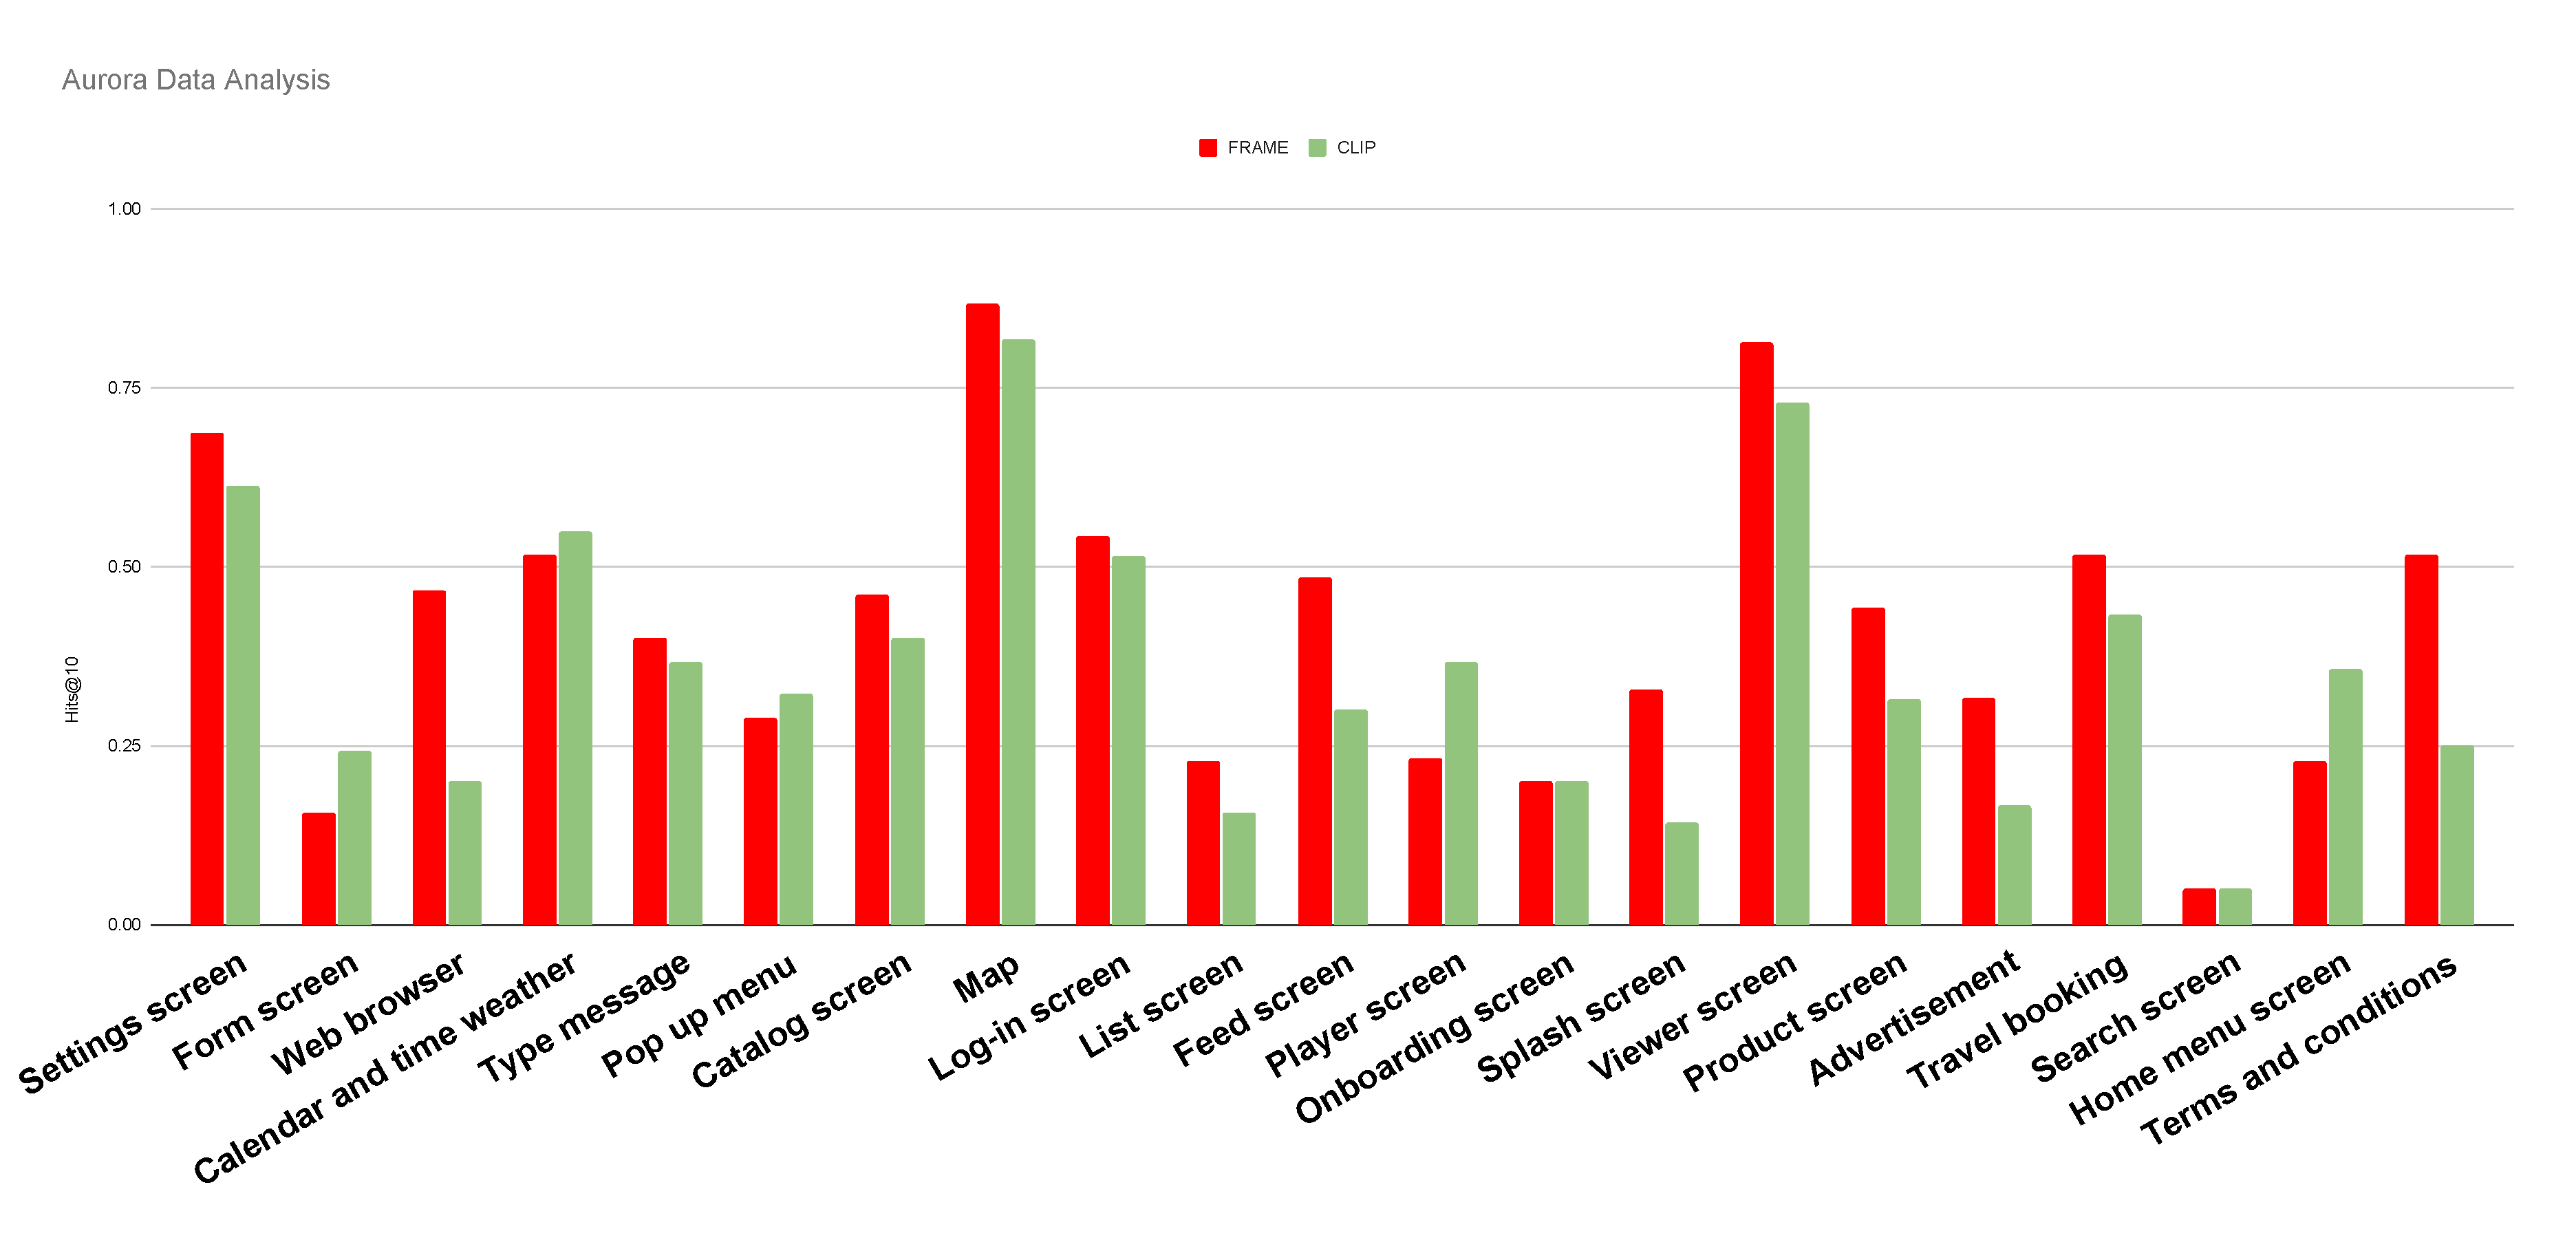
\includegraphics[width=0.75\textwidth]{imgs/AuroraCase.pdf}
    \caption{Visualization of FRAME vs CLIP Hits@10 on different screen types in the Aurora dataset}
    \label{fig:AuroraCase}
\end{figure}

Figure \ref{fig:AuroraCase} presents the difference between FRAME and CLIP embeddings on various screen types in the Aurora dataset. The bar chart shows \FRAME in red and CLIP in green. We see that \FRAME outperforms CLIP in every category except for four screen types. This gives \FRAME an advantage above CLIP in 17/21 screen categories. In the context of UI screen retrieval, the \FRAME embedding's advantage over CLIP embedding's performance across 17 out of 21 screen categories highlights \FRAME 's efficacy in capturing nuanced visual features specific to UI elements. \FRAME's performance in comparison to CLIP suggests that Frame embeddings are better suited for tasks requiring precise understanding and representation of static UI screens, potentially leading to improved retrieval accuracy and user experience in UI-related applications. 

\begin{figure}[h]
    \centering
    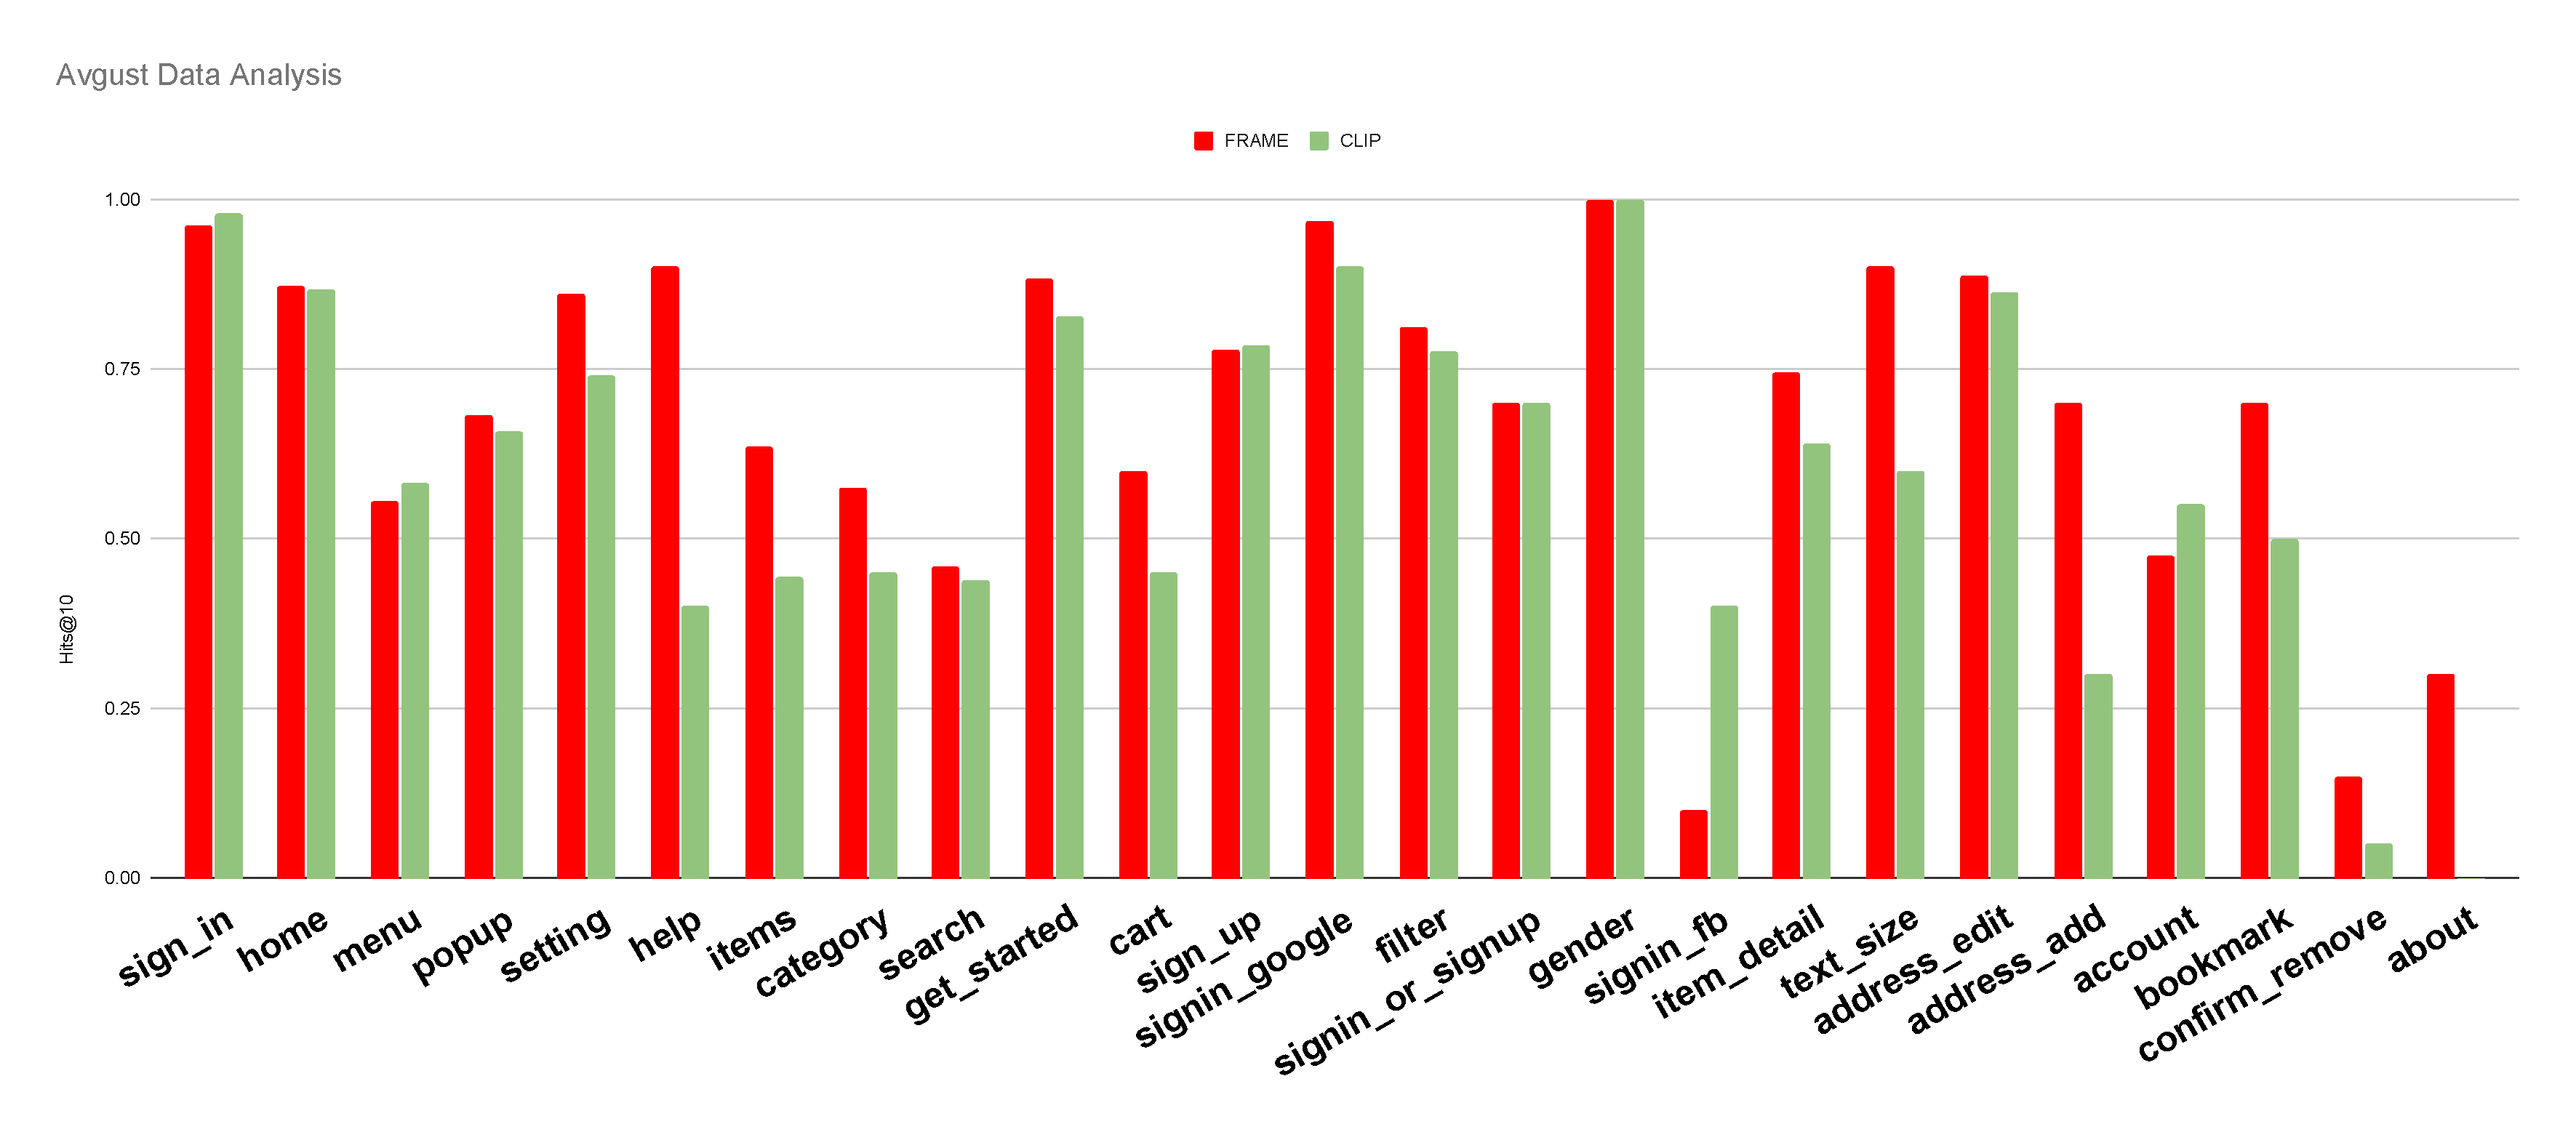
\includegraphics[width=0.75\textwidth]{imgs/AvgustCase.pdf}
    \caption{Visualization of FRAME vs CLIP Hits@10 on different screen types in the Avgust dataset}
    \label{fig:AvgustCase}    
\end{figure}

Figure \ref{fig:AuroraCase} presents the difference between FRAME and CLIP embeddings on various screen types in the Avgust dataset. The bar chart shows \FRAME in red and CLIP in green. We see that \FRAME outperforms CLIP in every category except for four screen types. This gives \FRAME an advantage above CLIP in 20/25 screen categories. In the context of UI screen retrieval, the \FRAME embedding's advantage over CLIP embedding's performance across 20 out of 25 screen categories highlights \FRAME 's efficacy in capturing nuanced visual features specific to UI elements. \FRAME's performance in comparison to CLIP suggests that Frame embeddings are better suited for tasks requiring precise understanding and representation of static UI screens, potentially leading to improved retrieval accuracy and user experience in UI-related applications. 


\subsubsection{\textbf{RQ$_3$} \textit{How important is the structural embedding propagation between graphs in order to enhance the embedding?}}


\FRAME creates a graph representation of the screen and augments weights within the nodes based on proximity and neighborhoods. This approach is designed to provide a set of weighted embeddings that can ingrain structural information into the embedding. To demonstrate the need for this propagation, we conduct an ablation study with six different variants of \FRAME, including and excluding various properties from the embedding. Table~\ref{AblatioTable} has the results for the ablation study for both datasets with each variant of \FRAME. \FRAME outperforms all variants of frame in every metric except for the version of frame that has the modified CLIP embedding and the propagated CLIP embedding in Hits@10 on the Aurora dataset. There are 6 variants of \FRAME. Table~\ref{AblatioTable} shows a comparison of \FRAME's results to all the variants.  
In the variants that do not have the larger augmented CLIP embedding and have one of the two possible propagated embeddings, Variants: NC-NPB-PC and NC-PB-NPC, we see poor performance. This poor performance can be attributed to the lack of broader screen information. These variants are solely dependent on the propagation between the icons or the text on the screen. 

In the variants that do have the larger augmented CLIP embedding and have one of the two possible propagated embeddings, Variants: C-NPB-PC and C-PB-NPC, we see an improved performance to the previous two variants. However, these variants still underperform when compared to the results for \FRAME. Given the lower performance of these two variants, it is assumed that the presence of both propagated is important to provide a higher structural context for the overall embedding. 

Given the results of the other four embeddings, \FRAME has two more configurations which offer a direct insight into the impact of the modified CLIP embedding and propagated embedding inclusion. 
The two main configurations to consider are NC-PB-PC and C-NPB-NPC. 

\begin{itemize}
  \item \textbf{NC-PB-PC}: This variant of \FRAME only has the propagated CLIP and BERT embedding. This is the information that ingrains the modified CLIP with structural information. However, on its own, the propagated embeddings are the fourth best variant of \FRAME. It outperforms the augmented version of CLIP which is just an image with no structural enhancements. This is shown in Table~\ref{AblatioTable}.
  \item \textbf{C-NPB-NPC}: This variant of \FRAME only has the augmented CLIP embedding without the propagated CLIP and BERT embeddings. This is the base image that is going to be enhanced with structural context. This variant of \FRAME is only the third best variant of \FRAME, only beating out the individual propagated CLIP and BERT embeddings, as shown in Table~\ref{AblatioTable}.
\end{itemize}

However, together, \FRAME can combine the two variants and leverage the properties of the augmented CLIP embedding and the structural properties of the propagated embeddings to create a structure-biased embedding. This results in \FRAME outperforming every variant of itself, demonstrating the impact of each element within the ablation process. 

\subsubsection{\textbf{RQ$_4$} \textit{How well does \FRAME leverage its ability to abstract the screen and disregard styling?}}
\begin{table}[h]
\centering
\renewcommand{\arraystretch}{1} % Adjust the row height
\scalebox{1}{
\begin{tabular}{|c|c|c|c|c|c|}
\toprule
\textbf{Dataset} & \textbf{Metrics} & \textbf{NB-C} & \textbf{NB-NC} & \textbf{B-NC} & \textbf{FRAME} \\
\hline
\midrule
\multirow{4}{*}{Aurora} 
& HR@1 & 0.4930 & 0.5347 & 0.5208 & \textbf{0.5625} \\
& HR@5 & 0.4069 & 0.4250 & 0.4527 & \textbf{0.4652} \\
& HR@10 & 0.3638 & 0.3805 & 0.4138 & \textbf{0.4166} \\
& MRR & 0.6171 & 0.6484 & 0.6492 & \textbf{0.6729} \\
\hline
\hline
\multirow{4}{*}{Avgust} 
& HR@1 & 0.8505 & 0.8784 & 0.8784 & \textbf{0.8823} \\
& HR@5 & 0.8119 & 0.8298 & 0.8266 & \textbf{0.8329} \\
& HR@10 & 0.7658 & 0.7827 & 0.7799 & \textbf{0.7827} \\
& MRR & 0.9094 & 0.9118 &  0.9138 &  \textbf{0.9184} \\
\bottomrule
\end{tabular}
}
\caption{Results over 2 datasets, where the best results are in \textbf{bold}, between FRAME and its variants including both contrast and black and white. }
\label{AugmentationTable}
\end{table}

\FRAME addresses color and style bias limitations in prior work by augmenting the image. There are three image preprocessing variants for the \FRAME embedding. The results for this augmentation ablation study are presented in Table~\ref{AugmentationTable}.

\subsubsubsec{NB-C}
This variant of \FRAME only increases the contrast on the input image. The results show that increasing the contrast on the input image is the least effective form of augmentation. As shown in Table~\ref{AblatioTable}, this variant of \FRAME is the least effective. 

\subsubsubsec{B-NC} 
This variant of \FRAME does not increase the contrast in the input image and only converts it to greyscale. The results show a noticeable increase in the performance of this variant, making it the highest-performing variant behind \FRAME. This variant benefits from the lack of color and allows the embedding to take on the structural aspects of the propagated embedding without allowing color bias to play a factor. 

\subsubsubsec{NB-NC}
This variant of \FRAME does not increase the contrast or make the image black-and-white. The results for this variant are interesting since it outperformed the contrast only variant. This gives an insight into how important the black-and-white is for the high contrast augmentation to define clear edges. 

Together with the inclusion of the black-and-white and high contrast modification, \FRAME can create an embedding that outperforms its variants while excluding color and increasing edge detection capabilities to define elements clearly on the screen. 


\FRAME is a novel approach to enhance existing image embeddings with structural information to embed UIs. There has been limited work in this area, so we present related work that has similar concepts to what \FRAME tries to achieve. We looked at previous work in UI Embeddings, UI Search and similarity, and Graph Based UI Representations. 

\subsection{Embedding Related Works}
There exists a limited body of work when considering embeddings for UI screens~\cite{Li21}, however, there have been increased efforts to provide a screen-specific embedding. 

One such effort is Screen2Vec, proposed by Li et al.~\cite{Li21}. Screen2Vec tackles the lack of UI Screen embeddings and proposes its own neural embeddings. Screen2Vec uses BERT text embeddings to take into account the text on the screen. Additionally, they use a layout embedding to embed the images with some layout information. Screen2Vec differs by creating their own embedding while using the Rico data~\cite{Rico} and uses the extracted screen hierarchy to embed screen hierarchy. This layout-based screen embedding is also employed by Deka et al. in Rico~\cite{Rico}. Both of these approaches use the same layout-based screen embedding which differs from the \FRAME proposes. These two embedding techniques aim to create a new embedding while \FRAME aims to enhance an existing embedding to be suitable for screen structure. 
\FRAME uses a computer vision approach to find the elements on the screen and use their positional information on the screen as opposed to finding elements within the screen hierarchy. \FRAME also utilizes a graph-based approach to creating layouts while considering both element visual and text characteristics within the graph. 

Li et al.~\cite{li2021vut} proposed VUT, a UI transformer for multimodal multi-task user interface modeling. This approach considered the hierarchical structure, image, and language properties of the screen to create their screen representations. VUT has two Transformer architectures, an Image-Structure model,
and a Question-Answer model. The image-structure model combines screenshot and view hierarchy data for UI encoding while the question-answer model encodes questions while attending to UI encodings from the Image-Structure model, generating text answers for language tasks and serving as the question encoder for grounding tasks to locate UI elements for action. However, \FRAME is a lightweight approach that takes existing embeddings and enhances them with structural properties and does not create its embedding using a transformer architecture. The structural properties of the screen in \FRAME are graph and visual position-based as opposed to hierarchy-based representation in VUT. VUT is an excellent baseline comparison for \FRAME, however, the model and architecture to use VUT are currently unavailable to the public. 

Bai et al.~\cite{bai2021uibert} proposed UIBert, a transformer-based joint image-text model to learn generic feature representations for a UI and its components~\cite{bai2021uibert}. This embedding is similar to VUT in its goal to create an embedding using image, text, and structural properties of the screen. Similar to VUT, UIBert also considers the view hierarchies for each screen and the leaf nodes. UIBert uses the element information on the screen in conjunction with the visual text to create an embedding with both textural and structural information. However, as discussed with VUT, UIBert is a new transformer-based embedding framework, whereas \FRAME enhances existing embeddings. Additionally, \FRAME interprets structure as visual positions on the GUI rather than an image's position in the hierarchy. UIBert may have provided an insight into the performance of \FRAME as a baseline, however, the models for UIBert are not available to the public. 

\subsubsubsec{UI Search and Similarity}
This paper presents a retrieval-motivated image embedding. It is important to consider other ways screen retrieval has been done ~\cite{Huang19, Bernal-Cardenas19, Chen20} and how \FRAME can be used to enhance search based on its retrieval-based evaluation. Guigleproposed by Bernal-Cardenas et al.~\cite{Bernal-Cardenas19} is a UI search engine. They use metadata information to facilitate a filter-based search. This method of finding embeddings is functional but does not provide and mbedding based search. Search is done through filters to find an image. 

GeminiScope proposed by Mao et al.~\cite{Mao18} proposed a GUI similarity metric that uses the leaf nodes in the hierarchy tree to determine the position of the elements on the screen. They compute the absolute values of UI-related features,
such as position and size, and use these metrics as their numerical representation for the screen. This allows them to perform distance calculations on the different images based on UI feature locations. \FRAME, like GeminiScope, considers the position of UI elements on the screen. However, GeminiScope does not consider the relations between the embeddings, unlike \FRAME. Additionally, \FRAME considers the text on the screen along with the actual visual representation of the icons. 

\subsubsubsec{UI Comprehension}
To modify or test a UI, it is necessary to have a semantic understanding of the UI. Many tools use the android screen hierarchy~\cite{bai2021uibert,li2021vut, Li21, Schoop22}, however, the hierarchy is not always available. We present a prior work that has used computer vision techniques to gain a semantic understanding of the elements on the screen. 
Spotlight, a tool introduced by Li et al.~\cite{li20spotlight} is a tool that uses computer vision to create a vision-language model architecture that can assist in screen comprehension tasks. Spotlight can generate text to suggest a screen or icon's function. This helps create lightweight icon detection for screens without a hierarchy. Following this line of thinking, we designed \FRAME to be hierarchy-free and use a computer vision approach to detect icons on the screen, resulting in an embedding that only needs a screenshot as input. 

Additionally, Schoop et al. ~\cite{Schoop22} proposed a technique to classify tappable icons on a screen given an image. This work is done by using XRAI. XRAI identifies and emphasizes influential areas within the input screenshot, which affect the prediction of capability for the chosen region. Additionally, it employs k-Nearest Neighbors to showcase mobile UIs from the dataset that exhibit contrasting influences on the perception of tappability. Though the intended application was not related to screen embedding creation, tappable icons can uncover important relations within the way the icons on a screen are laid out. \FRAME does not consider the tappability of the icon, however, it is a direction that can be considered. \FRAME is concerned with identifying niche relationships between icons and where they are positioned on the screen as opposed to their functionality. 

\subsubsubsec{Graph Based UI Representation}
Li et al. proposed Sugilite~\cite{Li20-suglite}, a graph-based UI element search for UI screens. Sugilite creates a UI snapshot graph using element metadata and position to identify each element on the screen. This allows users to write test scripts to test certain elements of the screen using natural language queries. WHile this is not an embedding, it utilizes a similar intuition to \FRAME by considering the graph-based approach to mapping elements. This method differs from \FRAME in two ways. Sugilite does not perform any structural relationship analysis between the different elements, they use the graph as a means to query the UI and find elements. Sugilite also uses metadata from the UI screens to create the graph. \FRAME aims be more versatile, therefore it creates an embedding for a screen from only the image of the screen. 

\subsection{Summary}
In this paper, we presented \FRAME, an approach for enhancing UI screen embeddings with structural information. We measured the performance and generalizability of \FRAME to various open source UIs. Our results indicate that \FRAME is effective in practice and outperforms key baselines, offering a novel approach to create vectors for UIs. Future work will examine the potential create embeddings for web apps and focus on creating an entirely new embedding as opposed to enhancing current ones.












% 
\section{Flaky Failure Logs: Study}
\label{sec:failureLogsStudy}

This is a summary of my study section in the paper currently under preparation.
% \jon{i would write "under preparation" until it is submitted}. \abdul{Done}


The detection of test flakiness can be achieved through various methods, and one such method is to debug failure logs, as highlighted in a study by Habchi et al. \cite{habchi2022qualitative}. Some developers might prefer this technique over others due to the fact that rerunning or using other detection methods could require significant resources and expertise. However, manual debugging can be a challenging approach, particularly when attempting to determine if a particular failure is due to flakiness or not. This is because the process can be time-consuming and demands a high level of skill and attention to detail in order to accurately identify if the failure is flaky or not. Failure logs can be particularly complex, especially in large and distributed systems, and require a deep understanding of the system's architecture, programming language, and all other dependencies to effectively analyze the logs.


Experienced developers may sometimes be able to identify whether a failure is flaky or not by examining the failure message and stacktrace, as discussed in a Gradle blog post on preventing flaky tests~\cite{gradlePreventingFlaky}.
This implies that developers can recognize flaky failures because they have encountered similar failures before, which means that flaky failures could be not unique in their failure exceptions. To gain a deeper understanding of this technique, I am currently analyzing the failure logs of flaky tests documented in Section~\ref{sec:flakeFlaggerStudy}. Specifically, my aim is to collect the failure logs from each reported flaky test in order to determine if each flaky failure, as indicated by its log, has been previously reported. The primary research questions I am addressing are as follows:


\begin{description}
  \item[\textbf{RQ1:}] Do flaky failures match for the same test across different executions of the test suite?
  \item[\textbf{RQ2:}] Do flaky failures match for different tests within the same execution of a test suite?

 \end{description}
 % \jon{Before going into the study design, I would suggest a paragraph or two right here describing what the implications of this study could be: if the answer to RQ1 and RQ2 is "yes", then how does that contribute to your overall goal?}\abdul{How about the following paragraph?}\jon{Looks great!}

By providing answers to the two research questions (RQs), developers can enhance their decision making process when it comes to utilizing logs to compare newly discovered failures with known flaky failures, in order to assess the potential flakiness of the new failures. The first RQ investigates whether a failure can be identified as flaky if its log matches previous flaky failures based on the failure exception and stacktrace lines. 
However, it should be noted that this does not necessarily imply that unique failures (failures that do not match any previously detected flaky failures) identified by their failure exception and stacktrace lines are not also flaky; they may simply not have been detected before. To address this aspect, the study aims to determine the proportion of unique failures in each flaky test that contains more than one flaky failure. The second RQ is formulated and discussed due to the occurrence of certain flakiness root causes that can lead to multiple tests failing simultaneously. For instance, if numerous tests share resources that may intermittently become unavailable, all dependent tests could fail. The study intends to assess the likelihood of flaky tests that fail concurrently sharing the same failure exception and stacktrace lines.

\newpage
\input{Listings/flakyFailure}
% \jon{Should line 3 end tag be </E>?}\abdul{Done}

 \subsection{Study Design}

To initiate this study, I collected the failure logs from the rerun experiment that was described in Section~\ref{sec:flakeFlaggerStudy}. For each flaky test, there was a collection of failure logs, with each log representing a specific failure that occurred during a particular run. I extracted the primary pieces of information that developers typically rely on when manually debugging from each failure log, which were the failure message and stacktrace lines. While the failure message in a log provides an overview of what went wrong in a test, examining the stacktrace lines is providing more details for identifying the root cause of a failure, as it provides a list of method calls that led to the failure. Both of them, in each failure, are used to generate an XML file for each flaky test, which contained all of its flaky failures. Each element in each test XML file corresponded to a specific type of failure based on its failure message and stacktrace lines.

% \jon{I suggest introducing 1-2 examples of failures here (before describing E/M/S), including the project name, test name, and complete exception/message/stacktrace. The following paragraphs can then reference back to those examples to explain what a "match" would be} \abdul{Next two paragraphs.}
% \jon{Looks great!}

Listing~\ref{lst:flakyFailures} shows two \emph{Failure} tags that correspond to two flaky failures reported in one of the tests of the \emph{alluxio} project. Each \emph{Failure} tag includes four primary sub-tags that describe each failure: test name (\textbf{T}), exception type (\textbf{E}), exception message (\textbf{M}), and stacktrace lines (\textbf{S}). The \textbf{T} tag provides the project to which the test belongs. The original failure message in the log follows the format of \textbf{E}:\textbf{M}, where \textbf{E} specifies the exception type (e.g., java.net.UnknownHostException), and \textbf{M} includes any text that comes after the exception. When analyzing the stacktrace lines (\textbf{S}), only the initial lines leading up to the test name are considered. This is because the top lines in a stacktrace represent the most recent method calls that were executed before the exception occurred and are often the ones most directly related to the root cause of the exception. The lower lines may still provide valuable information for debugging, but they are generally less relevant to the root cause of the exception. If the test name is not present in the stacktrace (such as failures occurring in the start or before methods in Listing~\ref{lst:flakyFailures}), the last line of the test class is taken as the final line from the stacktrace.


The failure message might contain distinct information associated with the specific time when the test fails. Consequently, when comparing two test failures using the elements (\textbf{E}), (\textbf{M}), and (\textbf{S}) as criteria, they may differ due to the unique information provided by the failure. For instance, the two failures shown in Listing\ref{lst:flakyFailures} could initially be perceived as separate failures, despite appearing identical except for the IP address mentioned in \textbf{M}. To compare two failures, I exclude the failure message \textbf{M} to prevent mismatched failures arising from this factor. While considering only \textbf{S} may not alter anything when comparing two failures, incorporating \textbf{E} provides additional information during the comparison of failures.





% \jon{I think that these two paragraphs clearly describes what you did, but does not completely capture why. Consider a reader who has no familiarity with flaky tests and matching failure logs. Why trim lines from the stacktrace? Why consider stacktraces at all? What would happen if you made different choices here?}\abdul{few updates in the previous paragraphs that hopefully capture Jon notes}\jon{Better now}



Various factors such as network or shared resources can cause test flakiness that impacts more than a single test, leading to multiple tests failing at the same time and producing similar failure logs. During manual debugging, developers may categorize a failure as flaky if it resembles a previous failure, even if it is not necessarily from the same test. To detect common failure logs, it is essential to compare failures from tests within the same test suite run, as well as failures from the same test. 
% Although it is possible to compare failure logs from two different projects, the domain of the two projects could impact the accuracy of matching. 
For the purpose of this study, I focus only on the two methods of comparing failures mentioned above. In the second method, when comparing failures, the stacktrace line that includes the failed test name is excluded to prevent mismatches due to differences only in the test name line.
% \jon{You are the one proposing these two methods here (not prior work) - can you provide some deeper discusion (at least a few sentences) of why it makes sense to consider these two methods, and whether there might be altenratives that you did not implement?} \abdul{Updated, but not sure if I captured the whole idea} \jon{Better now}


When dealing with a flaky test that exhibits multiple failures, I \emph{cluster} all failures based on the type of exception and stack trace lines. If there are two failures which have exactly the same exception type and stack trace lines, the expected to be in the same cluster. If a cluster consists only one failure, it is referred to as a unique cluster. Conversely, a non-unique cluster contains multiple failures. The uniqueness of a cluster indicates that the corresponding failure has been encountered only once, which implies challenges for developers when relying on previous knowledge. Equation~\ref{ScoreEq} quantifies the proportion of non-unique failures, providing a measure of the likelihood of similarities between these failures and other flaky failures.



% clustor instead of set 
\begin{equation}
    \label{ScoreEq}
  \text{NU score} = \frac{\text{Total number of non-unique clusters of failures}}{\text{Total number of failures clusters}}
\end{equation}




\subsection{Initial Study Result}

Table~\ref{tab:matchTable} presents a comprehensive overview of the study findings, containing three primary sections. The first column, labeled \emph{Total Flaky Tests and Failure}, provides fundamental statistical information derived from the collected failures including the number of studied flaky tests and the minimum, average, and maximum number of failures per test. 
The second column, titled \emph{Same Test Different Builds}, focuses on the matching of each test failure with other observed failures of the same test, in different test suite runs. 
I classify tests into six groups based on the number of flaky failures that we observed when running them 10,000 times.
For instance, tests that had flaky failures only twice belong to the group labeled \textbf{[2,3)}.
\sout{Then, for each of these groups, I provide the value \textbf{F}, which represents the total number of failure clusters from the tests in that group. Additionally, I calculate \textbf{NU} for each group of failure clusters.}
Then, I computer the value \textbf{S} exclusively for the first group, and \textbf{F} and \textbf{NU} for the remaining groups. \textbf{S} pertains to the total count of failure clusters arising from tests that experienced only one failure each. On the other hand, the term \textbf{F} represents the overall count of failure clusters resulting from the tests in each group, regardless to the number of failures within each cluster. The value \textbf{NU} corresponds to the percentage of clusters that contain at least two failures relative to the total number of clusters in the group.
The third column, titled as \emph{Different Tests Same Test Suite Run}, follows a similar computation method, but this time the grouping is based on the total number of failed tests in a single test suite run. For instance, if a test suite run encounters 3 failed tests, all the failures within that run are categorized into the group labeled \textbf{[3,10)}. As for the value of \textbf{F} in this column, it refers the clusters of failures within the grouped test suite runs.
\jon{I don't think that this explanation of the table clearly explains what the intervals mean in the header}\abdul{How about now? I feel that the description I want to deliver is too long to fit within the table's caption.}
\jon{This helps with the intervals. However: I think that the part that is still unclear is: are F and NU averages across all tests within that group? Or: are they totals across all of the tests?}\abdul{I rephrase it in order to be more clear. It is a total failure clusters from all tests within a group.}


\begin{table*}
\centering
\caption{How often do flaky test failures match other flaky failures.}
% \textnormal{ 1) Total Flaky Tests and Failures shows the number of flaky tests, and the failure frequency of those flaky test.\\
% 2) Matching each test failure against other observed failures of the same test (in different test suite run). We bucket each test by the number of test suite run that it failed in, and show the number of tests that failed that many times (F), and the percentage of failures of those tests that matched at least one other failure of the same test (called Non-Unique (NU)). \textbf{S} refers to a failure that has one single occurrence because a test only fails once.\\
% 3) Matching each test failure against a DIFFERENT test failure in the same test suite run as that failure. We bucket each test suite run by the total number of flaky test failures observed in that build, showing the total number of flaky tests that failed in test suite runs of that bucket (F), and the percentage of failures that matched at least one other failure in the same test suite run (NU). \textbf{S} refers to a test suite run that has one single flaky failure.\\ 
% 4) We chose to opt out the projects that have one flaky test reported in studied dataset. }}
% \jon{Generated by MatchingRatesPerTest.ipynb}
\footnotesize
\setlength{\tabcolsep}{2pt}
\resizebox{\textwidth}{!}{%
\begin{tabular}{lrrrr|rrrrrrrrrrr|rrrrrrrrr}
\toprule
\multicolumn{1}{c}{ } & \multicolumn{4}{c}{ Total Flaky Tests and Failures} & \multicolumn{11}{c}{Same Test Different Builds} & \multicolumn{9}{c}{Different Tests Same Test Suite Run} \\
\cmidrule(l{3pt}r{3pt}){2-5} \cmidrule(l{3pt}r{3pt}){6-16} \cmidrule(l{3pt}r{3pt}){17-25}
\multicolumn{2}{c}{ } & \multicolumn{3}{c}{Failures Per-Test} & [1] & \multicolumn{2}{c}{[2,3)}& \multicolumn{2}{c}{[3,10)} & \multicolumn{2}{c}{[10,100)} & \multicolumn{2}{c}{[100,1000)} & \multicolumn{2}{c}{[1000,10000)} & [1] &\multicolumn{2}{c}{[2,3)} & \multicolumn{2}{c}{[3,10)} & \multicolumn{2}{c}{[10,20)} & \multicolumn{2}{c}{[20,200)} \\
% \cmidrule(l{3pt}r{3pt}){4-6} \cmidrule(l{3pt}r{3pt}){7-8}  \cmidrule(l{3pt}r{3pt}){9-10} \cmidrule(l{3pt}r{3pt}){11-12} \cmidrule(l{3pt}r{3pt}){13-14} \cmidrule(l{3pt}r{3pt}){15-16} \cmidrule(l{3pt}r{3pt}){17-18} \cmidrule(l{3pt}r{3pt}){19-20} \cmidrule(l{3pt}r{3pt}){21-22}
 & Tests & Min & Avg & Max & S &F & NU &F & NU & F & NU & F & NU & F & NU & S & F & NU & F & NU & F & NU & F & NU \\
\midrule
spring-projects-spring-boot&163&1&1753&5525&16& & &19&74\%&32&91\%& & &299&100\%&4441&36&0\%& & &13&46\%&49844&78\%\\
\cellcolor{gray!6}{apache-hbase}&\cellcolor{gray!6}{145}&\cellcolor{gray!6}{1}&\cellcolor{gray!6}{716}&\cellcolor{gray!6}{2011}&\cellcolor{gray!6}{2}&\cellcolor{gray!6}{21}&\cellcolor{gray!6}{90\%}&\cellcolor{gray!6}{16}&\cellcolor{gray!6}{100\%}&\cellcolor{gray!6}{33}&\cellcolor{gray!6}{88\%}&\cellcolor{gray!6}{37}&\cellcolor{gray!6}{70\%}&\cellcolor{gray!6}{109}&\cellcolor{gray!6}{92\%}&\cellcolor{gray!6}{1263}&\cellcolor{gray!6}{252}&\cellcolor{gray!6}{17\%}&\cellcolor{gray!6}{3624}&\cellcolor{gray!6}{5\%}&\cellcolor{gray!6}{39654}&\cellcolor{gray!6}{71\%}&\cellcolor{gray!6}{ }&\cellcolor{gray!6}{ }\\
Alluxio-alluxio&116&1&51&168&0& & & & &166&94\%&17&94\%& & &721&13&8\%&3&67\%&15&73\%&1168&88\%\\
\cellcolor{gray!6}{square-okhttp}&\cellcolor{gray!6}{100}&\cellcolor{gray!6}{1}&\cellcolor{gray!6}{234}&\cellcolor{gray!6}{8539}&\cellcolor{gray!6}{31}&\cellcolor{gray!6}{3}&\cellcolor{gray!6}{33\%}&\cellcolor{gray!6}{57}&\cellcolor{gray!6}{89\%}&\cellcolor{gray!6}{4}&\cellcolor{gray!6}{100\%}&\cellcolor{gray!6}{9}&\cellcolor{gray!6}{100\%}&\cellcolor{gray!6}{17}&\cellcolor{gray!6}{94\%}&\cellcolor{gray!6}{1152}&\cellcolor{gray!6}{5910}&\cellcolor{gray!6}{3\%}&\cellcolor{gray!6}{15835}&\cellcolor{gray!6}{25\%}&\cellcolor{gray!6}{39}&\cellcolor{gray!6}{51\%}&\cellcolor{gray!6}{ }&\cellcolor{gray!6}{ }\\
apache-ambari&52&1&77&875&1& & &2&100\%&48&100\%&2&100\%& & &921&16&0\%& & &202&64\%& & \\
\cellcolor{gray!6}{hector-client-hector}&\cellcolor{gray!6}{33}&\cellcolor{gray!6}{43}&\cellcolor{gray!6}{198}&\cellcolor{gray!6}{5147}&\cellcolor{gray!6}{0}&\cellcolor{gray!6}{ }&\cellcolor{gray!6}{ }&\cellcolor{gray!6}{ }&\cellcolor{gray!6}{ }&\cellcolor{gray!6}{32}&\cellcolor{gray!6}{100\%}&\cellcolor{gray!6}{ }&\cellcolor{gray!6}{ }&\cellcolor{gray!6}{1}&\cellcolor{gray!6}{100\%}&\cellcolor{gray!6}{5145}&\cellcolor{gray!6}{50}&\cellcolor{gray!6}{0\%}&\cellcolor{gray!6}{ }&\cellcolor{gray!6}{ }&\cellcolor{gray!6}{87}&\cellcolor{gray!6}{99\%}&\cellcolor{gray!6}{ }&\cellcolor{gray!6}{ }\\
activiti-activiti&32&1&42&932&12&2&100\%&4&100\%&14&93\%&1&100\%& & &1281&98&2\%&3&0\%& & & & \\
\cellcolor{gray!6}{tootallnate-java-websocket}&\cellcolor{gray!6}{23}&\cellcolor{gray!6}{1}&\cellcolor{gray!6}{48}&\cellcolor{gray!6}{215}&\cellcolor{gray!6}{1}&\cellcolor{gray!6}{ }&\cellcolor{gray!6}{ }&\cellcolor{gray!6}{2}&\cellcolor{gray!6}{50\%}&\cellcolor{gray!6}{29}&\cellcolor{gray!6}{100\%}&\cellcolor{gray!6}{13}&\cellcolor{gray!6}{100\%}&\cellcolor{gray!6}{ }&\cellcolor{gray!6}{ }&\cellcolor{gray!6}{1139}&\cellcolor{gray!6}{435}&\cellcolor{gray!6}{26\%}&\cellcolor{gray!6}{265}&\cellcolor{gray!6}{54\%}&\cellcolor{gray!6}{ }&\cellcolor{gray!6}{ }&\cellcolor{gray!6}{ }&\cellcolor{gray!6}{ }\\
wildfly-wildfly&23&1&5&41&13& & &9&100\%&1&100\%& & & & &47&8&0\%&28&50\%& & & & \\
\cellcolor{gray!6}{qos-ch-logback}&\cellcolor{gray!6}{22}&\cellcolor{gray!6}{1}&\cellcolor{gray!6}{185}&\cellcolor{gray!6}{3824}&\cellcolor{gray!6}{6}&\cellcolor{gray!6}{5}&\cellcolor{gray!6}{60\%}&\cellcolor{gray!6}{2}&\cellcolor{gray!6}{100\%}&\cellcolor{gray!6}{8}&\cellcolor{gray!6}{100\%}&\cellcolor{gray!6}{1}&\cellcolor{gray!6}{100\%}&\cellcolor{gray!6}{1}&\cellcolor{gray!6}{100\%}&\cellcolor{gray!6}{3952}&\cellcolor{gray!6}{308}&\cellcolor{gray!6}{0\%}&\cellcolor{gray!6}{6}&\cellcolor{gray!6}{0\%}&\cellcolor{gray!6}{ }&\cellcolor{gray!6}{ }&\cellcolor{gray!6}{ }&\cellcolor{gray!6}{ }\\
apache-httpcore&22&1&16&162&9&5&100\%&6&100\%& & &2&100\%& & &346&8&0\%& & & & & & \\
\cellcolor{gray!6}{apache-incubator-dubbo}&\cellcolor{gray!6}{19}&\cellcolor{gray!6}{1}&\cellcolor{gray!6}{462}&\cellcolor{gray!6}{8849}&\cellcolor{gray!6}{2}&\cellcolor{gray!6}{4}&\cellcolor{gray!6}{100\%}&\cellcolor{gray!6}{9}&\cellcolor{gray!6}{100\%}&\cellcolor{gray!6}{3}&\cellcolor{gray!6}{100\%}&\cellcolor{gray!6}{1}&\cellcolor{gray!6}{100\%}&\cellcolor{gray!6}{1}&\cellcolor{gray!6}{100\%}&\cellcolor{gray!6}{8563}&\cellcolor{gray!6}{654}&\cellcolor{gray!6}{0\%}&\cellcolor{gray!6}{9}&\cellcolor{gray!6}{22\%}&\cellcolor{gray!6}{ }&\cellcolor{gray!6}{ }&\cellcolor{gray!6}{ }&\cellcolor{gray!6}{ }\\
kevinsawicki-http-request&18&1&194&246&3& & & & & & &15&100\%& & &0& & &3&67\%&735&67\%& & \\
\cellcolor{gray!6}{wro4j-wro4j}&\cellcolor{gray!6}{16}&\cellcolor{gray!6}{1}&\cellcolor{gray!6}{474}&\cellcolor{gray!6}{1803}&\cellcolor{gray!6}{1}&\cellcolor{gray!6}{ }&\cellcolor{gray!6}{ }&\cellcolor{gray!6}{2}&\cellcolor{gray!6}{100\%}&\cellcolor{gray!6}{7}&\cellcolor{gray!6}{71\%}&\cellcolor{gray!6}{1}&\cellcolor{gray!6}{100\%}&\cellcolor{gray!6}{12}&\cellcolor{gray!6}{100\%}&\cellcolor{gray!6}{382}&\cellcolor{gray!6}{227}&\cellcolor{gray!6}{0\%}&\cellcolor{gray!6}{6285}&\cellcolor{gray!6}{44\%}&\cellcolor{gray!6}{44}&\cellcolor{gray!6}{27\%}&\cellcolor{gray!6}{ }&\cellcolor{gray!6}{ }\\
undertow-io-undertow&7&1&8&54&0&2&0\%&7&86\%&3&100\%& & & & &92& & & & & & & & \\
\cellcolor{gray!6}{orbit-orbit}&\cellcolor{gray!6}{7}&\cellcolor{gray!6}{7}&\cellcolor{gray!6}{420}&\cellcolor{gray!6}{2546}&\cellcolor{gray!6}{0}&\cellcolor{gray!6}{ }&\cellcolor{gray!6}{ }&\cellcolor{gray!6}{1}&\cellcolor{gray!6}{100\%}&\cellcolor{gray!6}{3}&\cellcolor{gray!6}{100\%}&\cellcolor{gray!6}{2}&\cellcolor{gray!6}{100\%}&\cellcolor{gray!6}{1}&\cellcolor{gray!6}{100\%}&\cellcolor{gray!6}{2721}&\cellcolor{gray!6}{214}&\cellcolor{gray!6}{1\%}&\cellcolor{gray!6}{5}&\cellcolor{gray!6}{20\%}&\cellcolor{gray!6}{ }&\cellcolor{gray!6}{ }&\cellcolor{gray!6}{ }&\cellcolor{gray!6}{ }\\
doanduyhai-Achilles&4&1&26&60&1& & & & &3&100\%& & & & &103&2&0\%& & & & & & \\
\cellcolor{gray!6}{elasticjob-elastic-job-lite}&\cellcolor{gray!6}{3}&\cellcolor{gray!6}{1}&\cellcolor{gray!6}{2}&\cellcolor{gray!6}{4}&\cellcolor{gray!6}{2}&\cellcolor{gray!6}{ }&\cellcolor{gray!6}{ }&\cellcolor{gray!6}{2}&\cellcolor{gray!6}{50\%}&\cellcolor{gray!6}{ }&\cellcolor{gray!6}{ }&\cellcolor{gray!6}{ }&\cellcolor{gray!6}{ }&\cellcolor{gray!6}{ }&\cellcolor{gray!6}{ }&\cellcolor{gray!6}{5}&\cellcolor{gray!6}{1}&\cellcolor{gray!6}{100\%}&\cellcolor{gray!6}{ }&\cellcolor{gray!6}{ }&\cellcolor{gray!6}{ }&\cellcolor{gray!6}{ }&\cellcolor{gray!6}{ }&\cellcolor{gray!6}{ }\\
alibaba-fastjson&3&4&49&121&0& & &2&100\%& & &2&100\%& & &191&4&0\%& & & & & & \\
\cellcolor{gray!6}{zxing-zxing}&\cellcolor{gray!6}{2}&\cellcolor{gray!6}{322}&\cellcolor{gray!6}{352}&\cellcolor{gray!6}{382}&\cellcolor{gray!6}{0}&\cellcolor{gray!6}{ }&\cellcolor{gray!6}{ }&\cellcolor{gray!6}{ }&\cellcolor{gray!6}{ }&\cellcolor{gray!6}{ }&\cellcolor{gray!6}{ }&\cellcolor{gray!6}{2}&\cellcolor{gray!6}{100\%}&\cellcolor{gray!6}{ }&\cellcolor{gray!6}{ }&\cellcolor{gray!6}{694}&\cellcolor{gray!6}{10}&\cellcolor{gray!6}{0\%}&\cellcolor{gray!6}{ }&\cellcolor{gray!6}{ }&\cellcolor{gray!6}{ }&\cellcolor{gray!6}{ }&\cellcolor{gray!6}{ }&\cellcolor{gray!6}{ }\\
\bottomrule
\label{tab:matchTable}
\end{tabular}
}
\end{table*}




% RQ1 
\textbf{RQ1: Do flaky failures match for the same test across different executions of the test suite?} In Table~\ref{tab:matchTable}, the result per each project has been computed. For instance, the first row is a summary of the project \spring. Among the 10,000 trials, there are 163 flaky tests that have failed an average of 1753 times. Within these 163 failures, I observe the following distribution of failure clusters: 16 failure clusters consist of tests that failed only once, 19 failure clusters from tests that failed between 3 to 10 times (\textbf{[3-10)}), 32 failure clusters from tests that failed between 10 to 100 times (\textbf{[10-100)}), and 299 failure clusters from tests that failed more than 1,000 times.
Of the 19 failure clusters in the group \textbf{[3-10)}, 74\% of them contain at least two failures, indicating that the remaining clusters only have a single failure.
In terms of the \emph{Different Tests Same Test Suite Run} column in the first row, I found 4,441 test suite runs that include only one failed test. Additionally, there are 36 failure clusters from test suite runs with two failed tests, and none of these clusters have more than one failure (0\%).
% \jon{Given the complexity of the table, I would suggest quickly providing one or two example findings in prose. Example:
% For example, in the first row, we can see that there were 163 flaky tests, failing an average of 1,753 times (out of the 10,000 trials).
% Of those failures, there are 16 unique failure clusters, 19 failure clusters that match 3-10...}\abdul{How about now?}
% \jon{this is better, thanks.}


% Generally, there is an increase in non-unique failures across multiple projects, by finding many projects with 100\% scores.
In numerous projects, a consistent primary observation is that the non-unique proportion (\textbf{NU}) reaches 100\% in the \emph{Same Test Different Builds} results, implying that flaky failures frequently occur. This finding supports the idea that developers often depend on their past experiences with flaky failures to help them identifying these failures flakiness.
\jon{I don't understand this sentence. Is the meaning: results for NU across projects are quite similar?}
\abdul{I meant that the concept of NU is not detected only in one project indicating that this could be usefull approach regardless to the project domain.}
\jon{Here is some proposed new text:
A key finding is that, for many projects, the non-unique proportion (NU) is 100\% in the ``Same Test Different Builds'' configuration, implying that flaky failures often repeat.
This is important because...}\abdul{How about now}
Another notable finding is that tests experiencing frequent flakiness do not always exhibit similarities among their failures consistently. For example, approximately 30\% of the flaky failures that occur more than 100 times in \emph{hbase} are classified as unique failure clusters. On the other hand, within the same project, there are no unique clusters among failures that exhibit flakiness less than 10 times. This prompts me to conduct a comprehensive analysis of the factors contributing to the occurrence of unique failure clusters.

According to the study findings, there are a total of 101 failure clusters that are classified as unique across all projects. These unique failures contribute to a decrease in UN scores. Among these clusters, 82 of them are considered unique because they differ either in the exception type, the line from the stack trace that begins with the test name, or both. These cases indicate entirely distinct failures, as each one is associated with a different line of test code. In comparison to the non-unique failures, I am investigating whether specific factors, such as test complexity or the type of exception, could be connected to the presence of unique failure clusters. Alternatively, it is possible that uniqueness occurs independently and may be related to the underlying causes of flakiness in general.

I have examined three factors, namely test length, the number of lines in the stack traces, and the total number of assertion statements, to assess the complexity of each flaky test. Using these factors, I conducted an analysis of both unique and non-unique failures to investigate potential connections with specific clusters.
For instance, in the \emph{java-websocket} project, the only unique failure cluster exhibited a significantly larger number of lines in the test body compared to all tests associated with non-unique failure clusters (79 lines versus a maximum of 3 lines). In the \emph{spring-boot} project, it was observed that all unique failure clusters had a median of 73 stack trace lines, while considering both unique and non-unique failure clusters resulted in a median of 4 stack trace lines. Additionally, in the \emph{undertwo} project, there were two distinct tests with unique failure clusters, and these tests shared the highest number of assertion statements when compared to other tests.
\sout{Overall, there is no single factor among these that consistently correlates with unique failure clusters across all projects. However, the impact of these factors varies from one project to another. This analysis provides valuable insights into the relationship between test complexity factors and the occurrence of unique failure clusters.}
In general, no single factor consistently correlates with unique failure clusters across all projects, as the impact of these factors varies from one project to another. It is crucial to avoid relying on a single factor to determine the uniqueness of a failure. Instead, it is essential to examine multiple factors when necessary. By doing so, a more comprehensive and accurate assessment of failure uniqueness can be achieved, taking into account the specific characteristics of each individual project.
\jon{The valuable insights are not clear to me - it seemed more like there was no clear pattern/finding?}\abdul{I may not explain it well, I try to see if there is a specific pattern between having unique failure with some discussed factors.}
\jon{Can you add a sentence or two explaining why it is a valuable insight to see that there is no pattern between these factors? The implications of this are not otherwise motivated in the preceeding text.}\abdul{How clear is it now?}


Regarding exceptions, I discovered that the \emph{java.lang.IllegalArgumentException} is detecting in 5 unique clusters in two different projects (\emph{Alluxio} and \emph{hbase}, while in \emph{hbase}, it is associated with also a non-unique cluster in only one case. Interestingly, all these tests with unique clusters also have non-failure clusters linked to the \emph{UnknownHostException}. This suggests that considering the correlation among failures per test can help establish connections between the project domain and failures. It is possible that some exceptions occur due to infrequent causes of flakiness. For instance, in the \emph{wro4j} project, there are only two unique failure exceptions, originating from separate tests, but sharing the same type of failure exception (\emph{java.net.SocketTimeoutException}). Upon conducting a comprehensive analysis, I noticed that these two unique failures occurred consecutively during test suite runs and exhibited similar stack trace lines, except for the lines specific to the respective tests involved. 

To enhance the analysis of exceptions in relation to their occurrence in unique and non-unique failures, I gathered data on the various exception types present in all unique failures. For each exception type, I then determined the frequency of its appearance in non-unique failures, as indicated in Table~\ref{table:uniqueExceptions}. This investigation aimed to identify exceptions that might be closely associated with causing unique failures.
From a total of 72 unique clusters, I identified 16 different exceptions. Among these exceptions, only two, namely \emph{java.lang.IllegalArgumentException} and \emph{java.net.SocketTimeoutException}, were more observed in unique clusters than in non-unique ones. However, it is also occurred once in non-unique failures even for these two exceptions. 
Despite examining these exceptions, it remains challenging to establish a direct link between the uniqueness of a failure and the specific type of exception. Furthermore, I observed that even in exceptions that are specific to a particular project, like \emph{org.apache.hadoop.hbase.client.NoServerForRegionException}, cannot be definitively linked to the cause of uniqueness.  
\jon{What about including the analysis of exception types in this proposal, or, describing it as future work?}\abdul{I have not discussed it here. I discuss only the exception type when we compare flaky with non flaky? If you think it is good to be discussed here, I can provide 1-2 paragraphs here. }
\jon{I think that it is interesting and relevant to discuss here, too.} \abdul{I added this paragraph to briefly discuss the relationship between the uniqueness and exception type. Any further comments here?}




% This is similar to the Table~\ref{nonunique}, but for the failures that flakes once (which have no match with other flaky failures). For the columns \textit{Failures Flake =1}: it shows the number of failures that flakes once (\textbf{f}), follow by the total number of tests where these failures belong (\textbf{t}), followed by the number of tests where the whole test only flakes once (\textbf{t_{1}})

\begin{table*}[t]
\caption[Top 10 Most Occurrence Exception in Flaky and True Failures]{Top 10 Most Occurrence Exception in Flaky and True Failures \\ 
\textnormal{ The \textit{Exception Occurrence} column details the frequency of a specific exception, indicating in how many projects, tests, and failures this exception has been observed. The \textit{Match Result (with Stacktraces)} column displays the match distributions, considering stacktraces and the related test count while the, \textit{Match Result (without Stacktraces)} column indicates match results based on exception types, excluding stacktraces.}}

\vspace{-5pt}
\setlength{\tabcolsep}{2.5pt}
\newcommand{\failureRateWidth}{2.5in}
\newcommand{\failureRateHeight}{4em}
\scriptsize
\centering

% -- > Version 2: With Tests .. 

    \begin{tabular}{l|rrr|rr|rrrr|rrrr}
    \toprule
      & \multicolumn{5}{c|}{\textbf{Exception Occurrence}} & \multicolumn{4}{c|}{\textbf{Match Result by Failures}} & \multicolumn{4}{c}{\textbf{Match Result by Failures}} \\ 

      & \multicolumn{5}{c|}{\textbf{}} & \multicolumn{4}{c|}{\textbf{(with Stacktraces)}}  &\multicolumn{4}{c}{\textbf{(without Stacktraces)}} \\ 
     
     \textbf{Exception Name}&\textbf{Projects}&\textbf{Tests}&\textbf{Failures}&\textbf{True}&\textbf{Flaky}&\textbf{TP}& \textbf{FN}&\textbf{FP}& \textbf{TN}&\textbf{TP}& \textbf{FN}&\textbf{FP}& \textbf{TN}\\
        \midrule
AssertionError&21&407&51,453&20,507&30,946&6,120&24,826&4,850&15,657&64&30,550&13,968&6,539\\

\cellcolor{gray!6}{NullPointerException}&\cellcolor{gray!6}{22}&\cellcolor{gray!6}{498}&\cellcolor{gray!6}{49,906}&\cellcolor{gray!6}{41,709}&\cellcolor{gray!6}{8,197}&\cellcolor{gray!6}{1,644}&\cellcolor{gray!6}{6,553}&\cellcolor{gray!6}{449}&\cellcolor{gray!6}{41,260}&\cellcolor{gray!6}{34}&\cellcolor{gray!6}{8,163}&\cellcolor{gray!6}{7,913}&\cellcolor{gray!6}{33,796}\\
IOException&7&257&20,097&15,963&4,134&3,614&520&519&15,444&28&3,141&3,717&12,246\\
\cellcolor{gray!6}{RuntimeException}&\cellcolor{gray!6}{17}&\cellcolor{gray!6}{420}&\cellcolor{gray!6}{13,810}&\cellcolor{gray!6}{13,676}&\cellcolor{gray!6}{134}&\cellcolor{gray!6}{43}&\cellcolor{gray!6}{91}&\cellcolor{gray!6}{1,011}&\cellcolor{gray!6}{12,665}&\cellcolor{gray!6}{31}&\cellcolor{gray!6}{103}&\cellcolor{gray!6}{1,141}&\cellcolor{gray!6}{12,535}\\
NoServerForRegionException&1&35&11,686&169&11,517&11,512&5&0&169&1,921&9,596&75&94\\
\cellcolor{gray!6}{UnknownHostException}&\cellcolor{gray!6}{9}&\cellcolor{gray!6}{234}&\cellcolor{gray!6}{9,942}&\cellcolor{gray!6}{319}&\cellcolor{gray!6}{9,623}&\cellcolor{gray!6}{9,620}&\cellcolor{gray!6}{3}&\cellcolor{gray!6}{0}&\cellcolor{gray!6}{319}&\cellcolor{gray!6}{9,620}&\cellcolor{gray!6}{3}&\cellcolor{gray!6}{0}&\cellcolor{gray!6}{319}\\
ActivitiException&1&30&9,893&9,821&72&0&72&614&9,207&0&72&3,094&6,727\\
\cellcolor{gray!6}{IllegalArgumentException}&\cellcolor{gray!6}{17}&\cellcolor{gray!6}{401}&\cellcolor{gray!6}{9,052}&\cellcolor{gray!6}{9,049}&\cellcolor{gray!6}{3}&\cellcolor{gray!6}{0}&\cellcolor{gray!6}{3}&\cellcolor{gray!6}{190}&\cellcolor{gray!6}{8,859}&\cellcolor{gray!6}{0}&\cellcolor{gray!6}{3}&\cellcolor{gray!6}{212}&\cellcolor{gray!6}{8,837}\\
AssertionFailedError&7&98&8,832&7,054&1,778&66&1,712&1,648&5,406&66&1,712&4,150&2,904\\
\cellcolor{gray!6}{PersistenceException}&\cellcolor{gray!6}{2}&\cellcolor{gray!6}{30}&\cellcolor{gray!6}{8,581}&\cellcolor{gray!6}{8,580}&\cellcolor{gray!6}{1}&\cellcolor{gray!6}{0}&\cellcolor{gray!6}{1}&\cellcolor{gray!6}{164}&\cellcolor{gray!6}{8,416}&\cellcolor{gray!6}{0}&\cellcolor{gray!6}{1}&\cellcolor{gray!6}{398}&\cellcolor{gray!6}{8,182}\\



%     \begin{tabular}{l|rrr|rr|rrrr|rrrr|rrrr|rrrr}
%     \toprule
%       & \multicolumn{5}{c|}{\textbf{Exception Occurrence}} & \multicolumn{8}{c|}{\textbf{Match Result (with Stacktraces)}} & \multicolumn{8}{c}{\textbf{Match Result (without Stacktraces)}} \\ 

%       & \multicolumn{5}{c|}{\textbf{}} & \multicolumn{4}{c|}{\textbf{By Failures}} & \multicolumn{4}{c|}{\textbf{By Tests}} & \multicolumn{4}{c}{\textbf{By Tests}} & \multicolumn{4}{c}{\textbf{By Failures}} \\ 
     
%      \textbf{Exception Name}&\textbf{Projects}&\textbf{Tests}&\textbf{Failures}&\textbf{True}&\textbf{Flaky}&\textbf{TP}& \textbf{FN}&\textbf{FP}& \textbf{TN}&\textbf{TP}& \textbf{FN}&\textbf{FP}& \textbf{TN}&\textbf{TP}& \textbf{FN}&\textbf{FP}& \textbf{TN}&\textbf{TP}& \textbf{FN}&\textbf{FP}& \textbf{TN}\\
%         \midrule
% AssertionError&21&407&51,453&20,507&30,946&6,120&24,826&4,850&15,657&64&122&96&371&396&30,550&13,968&6,539&5&176&173&226\\
% \cellcolor{gray!6}{NullPointerException}&\cellcolor{gray!6}{22}&\cellcolor{gray!6}{498}&\cellcolor{gray!6}{49,906}&\cellcolor{gray!6}{41,709}&\cellcolor{gray!6}{8,197}&\cellcolor{gray!6}{1,644}&\cellcolor{gray!6}{6,553}&\cellcolor{gray!6}{449}&\cellcolor{gray!6}{41,260}&\cellcolor{gray!6}{32}&\cellcolor{gray!6}{100}&\cellcolor{gray!6}{99}&\cellcolor{gray!6}{489}&\cellcolor{gray!6}{34}&\cellcolor{gray!6}{8,163}&\cellcolor{gray!6}{7,913}&\cellcolor{gray!6}{33,796}&\cellcolor{gray!6}{9}&\cellcolor{gray!6}{120}&\cellcolor{gray!6}{120}&\cellcolor{gray!6}{369}\\
% IOException&7&257&20,097&15,963&4,134&3,614&520&519&15,444&28&19&13&234&993&3,141&3,717&12,246&19&27&22&212\\
% \cellcolor{gray!6}{RuntimeException}&\cellcolor{gray!6}{17}&\cellcolor{gray!6}{420}&\cellcolor{gray!6}{13,810}&\cellcolor{gray!6}{13,676}&\cellcolor{gray!6}{134}&\cellcolor{gray!6}{43}&\cellcolor{gray!6}{91}&\cellcolor{gray!6}{1,011}&\cellcolor{gray!6}{12,665}&\cellcolor{gray!6}{7}&\cellcolor{gray!6}{14}&\cellcolor{gray!6}{2}&\cellcolor{gray!6}{409}&\cellcolor{gray!6}{31}&\cellcolor{gray!6}{103}&\cellcolor{gray!6}{1,141}&\cellcolor{gray!6}{12,535}&\cellcolor{gray!6}{5}&\cellcolor{gray!6}{16}&\cellcolor{gray!6}{12}&\cellcolor{gray!6}{399}\\
% NoServerForRegionException&1&35&11,686&169&11,517&11,512&5&0&169&8&4&0&33&1,921&9,596&75&94&2&9&9&24\\
% \cellcolor{gray!6}{UnknownHostException}&\cellcolor{gray!6}{9}&\cellcolor{gray!6}{234}&\cellcolor{gray!6}{9,942}&\cellcolor{gray!6}{319}&\cellcolor{gray!6}{9,623}&\cellcolor{gray!6}{9,620}&\cellcolor{gray!6}{3}&\cellcolor{gray!6}{0}&\cellcolor{gray!6}{319}&\cellcolor{gray!6}{133}&\cellcolor{gray!6}{3}&\cellcolor{gray!6}{0}&\cellcolor{gray!6}{98}&\cellcolor{gray!6}{9,620}&\cellcolor{gray!6}{3}&\cellcolor{gray!6}{0}&\cellcolor{gray!6}{319}&\cellcolor{gray!6}{133}&\cellcolor{gray!6}{3}&\cellcolor{gray!6}{0}&\cellcolor{gray!6}{98}\\
% ActivitiException&1&30&9,893&9,821&72&0&72&614&9,207&0&9&7&29&0&72&3,094&6,727&0&9&8&21\\
% \cellcolor{gray!6}{IllegalArgumentException}&\cellcolor{gray!6}{17}&\cellcolor{gray!6}{401}&\cellcolor{gray!6}{9,052}&\cellcolor{gray!6}{9,049}&\cellcolor{gray!6}{3}&\cellcolor{gray!6}{0}&\cellcolor{gray!6}{3}&\cellcolor{gray!6}{190}&\cellcolor{gray!6}{8,859}&\cellcolor{gray!6}{0}&\cellcolor{gray!6}{3}&\cellcolor{gray!6}{3}&\cellcolor{gray!6}{401}&\cellcolor{gray!6}{0}&\cellcolor{gray!6}{3}&\cellcolor{gray!6}{212}&\cellcolor{gray!6}{8,837}&\cellcolor{gray!6}{0}&\cellcolor{gray!6}{3}&\cellcolor{gray!6}{3}&\cellcolor{gray!6}{398}\\
% AssertionFailedError&7&98&8,832&7,054&1,778&66&1,712&1,648&5,406&1&21&21&94&66&1,712&4,150&2,904&1&21&21&76\\
% \cellcolor{gray!6}{PersistenceException}&\cellcolor{gray!6}{2}&\cellcolor{gray!6}{30}&\cellcolor{gray!6}{8,581}&\cellcolor{gray!6}{8,580}&\cellcolor{gray!6}{1}&\cellcolor{gray!6}{0}&\cellcolor{gray!6}{1}&\cellcolor{gray!6}{164}&\cellcolor{gray!6}{8,416}&\cellcolor{gray!6}{0}&\cellcolor{gray!6}{1}&\cellcolor{gray!6}{1}&\cellcolor{gray!6}{30}&\cellcolor{gray!6}{0}&\cellcolor{gray!6}{1}&\cellcolor{gray!6}{398}&\cellcolor{gray!6}{8,182}&\cellcolor{gray!6}{0}&\cellcolor{gray!6}{1}&\cellcolor{gray!6}{1}&\cellcolor{gray!6}{29}\\

\bottomrule


\end{tabular}
\label{table:exceptions}
\vspace{-10pt}
\end{table*}




% \begin{table}[t]
%   \setlength{\tabcolsep}{2.0pt}

% % \jon{Resized table to try to fit bigger column headers. Not clear what unique means. Unique by stack trace?}
% \caption{List of top 10 Exceptions in Flaky Failures. \\
% \textnormal{\emph{Total Failure} indicates the count of each exception's occurrences and the total projects where these exceptions appear. \emph{With S} and \emph{Without S} represent the presence or absence of stacktrace lines during the matching using the \syntax, respectively. \emph{TP} refers to failures not matching any non-flaky failures, while \emph{FN} refers flaky failures that match with at least one non-flaky failure.}}
% \label{table:exceptions}
% \vspace{-4pt}
% %\resizebox{\textwidth}{!}{
% % \scriptsize
% \footnotesize
% \begin{tabular}{l|rr|rr|rr}

% \toprule
%       & \multicolumn{2}{c|}{\textbf{Total Failures}} & \multicolumn{2}{c|}{\textbf{With S}} & \multicolumn{2}{c}{\textbf{Without S}}\\
      

% \textbf{Exceptions} & \textbf{F} & \textbf{P}  & \textbf{TP} & \textbf{FN}  & \textbf{TP} & \textbf{FN} \\
% \midrule
% % AssertionError&186&15&88&98&8&178\\
% % \cellcolor{gray!6}{NullPointerException}&\cellcolor{gray!6}{185}&\cellcolor{gray!6}{5}&\cellcolor{gray!6}{39}&\cellcolor{gray!6}{146}&\cellcolor{gray!6}{9}&\cellcolor{gray!6}{176}\\
% % UnknownHostException&136&6&136&0&136&0\\
% % \cellcolor{gray!6}{IOException}&\cellcolor{gray!6}{70}&\cellcolor{gray!6}{4}&\cellcolor{gray!6}{57}&\cellcolor{gray!6}{13}&\cellcolor{gray!6}{36}&\cellcolor{gray!6}{34}\\
% % ProvisionException&49&1&49&0&0&49\\
% % \cellcolor{gray!6}{HCassandraInternalException}&\cellcolor{gray!6}{31}&\cellcolor{gray!6}{1}&\cellcolor{gray!6}{31}&\cellcolor{gray!6}{0}&\cellcolor{gray!6}{31}&\cellcolor{gray!6}{0}\\
% % SocketException&31&1&29&2&1&30\\
% % \cellcolor{gray!6}{Exception}&\cellcolor{gray!6}{30}&\cellcolor{gray!6}{5}&\cellcolor{gray!6}{30}&\cellcolor{gray!6}{0}&\cellcolor{gray!6}{28}&\cellcolor{gray!6}{2}\\
% % RuntimeException&23&3&21&2&9&14\\
% % \cellcolor{gray!6}{AssertionFailedError}&\cellcolor{gray!6}{22}&\cellcolor{gray!6}{5}&\cellcolor{gray!6}{1}&\cellcolor{gray!6}{21}&\cellcolor{gray!6}{1}&\cellcolor{gray!6}{21}\\


% AssertionError&30946&19&6149&24797&399&30547\\
% \cellcolor{gray!6}{NoServerForRegionException}&\cellcolor{gray!6}{11517}&\cellcolor{gray!6}{1}&\cellcolor{gray!6}{11517}&\cellcolor{gray!6}{0}&\cellcolor{gray!6}{1921}&\cellcolor{gray!6}{9596}\\
% UnknownHostException&9623&6&9623&0&9623&0\\
% \cellcolor{gray!6}{NoSuchMethodError}&\cellcolor{gray!6}{8539}&\cellcolor{gray!6}{1}&\cellcolor{gray!6}{8539}&\cellcolor{gray!6}{0}&\cellcolor{gray!6}{8539}&\cellcolor{gray!6}{0}\\
% NullPointerException&8197&5&1647&6550&34&8163\\
% \cellcolor{gray!6}{WroRuntimeException}&\cellcolor{gray!6}{6487}&\cellcolor{gray!6}{1}&\cellcolor{gray!6}{0}&\cellcolor{gray!6}{6487}&\cellcolor{gray!6}{0}&\cellcolor{gray!6}{6487}\\
% SocketException&4547&1&4492&55&3&4544\\
% \cellcolor{gray!6}{IOException}&\cellcolor{gray!6}{4134}&\cellcolor{gray!6}{4}&\cellcolor{gray!6}{3620}&\cellcolor{gray!6}{514}&\cellcolor{gray!6}{998}&\cellcolor{gray!6}{3136}\\
% ExecutionException&3465&1&0&3465&0&3465\\
% \cellcolor{gray!6}{ProvisionException}&\cellcolor{gray!6}{3055}&\cellcolor{gray!6}{1}&\cellcolor{gray!6}{3055}&\cellcolor{gray!6}{0}&\cellcolor{gray!6}{0}&\cellcolor{gray!6}{3055}\\
% \bottomrule
% \end{tabular}
% \vspace{-10pt}
% \end{table}

 
In general, it is common for newly detected flaky failures to have matches with previously known detected failures. This practice helps in identifying recurring patterns and establishing a connection between similar failures. However, there are cases where a failure does not have a previous match. Cases where flaky failures have no common cause or previous match require additional investigation to understand their underlying causes. The study findings suggest that these unique cases do not have a shared or identifiable cause among them.

% One of the observed factors is when the failed test is complex e.g. contains multiple assertion statements, which is subject to have many failures with different stack trace lines. 
% For example, a flaky test in the "okhttp" project demonstrates this behavior by having three different assertion statements. \jon{I'm not sure what this is trying to say - that the reason why it doesn't match is because there are many different assertions that could fail?} \abdul{Yes, this is what I want to say, but the example sounds weak. I am thinking to study the correlation between the test size ( Test Lines of Code numbers from FlakeFlagger dataset)}
% \sout{We have not identified any particular projects that exhibit a higher occurrence of non-unique failures compared to others.}  \jon{Is apache-hbase different than the others? Or wro4j? The numbers seem the most different for these projects compard to the others, and maybe we should mention this along with a 1-2 sentence explanation for why that might be.} \abdul{I am working on finding why apache-hbase has many unique failure clusters.}
% \sout{This leads us to the conclusion that non-unique failures are not specifically tied to the nature of the project itself. However, we have observed that there are four projects with over 10 tests that exhibit flakiness, occurring once. In these projects, a significant portion of the flaky tests, even those that exhibit flakiness multiple times, have unique failures.}
% I noticed that most of the flaky tests in Spring-boot failed more than half of the total number of runs and none of these failures have been reported as a unique failure. With a close look, we have founds that around third-quarter of the failures comes from the \emph{parameterized} tests. 






% DQ2
\textbf{RQ2: Do flaky failures match for different tests within the same execution of a test suite?} The main observation from the \emph{Different Tests Same Test Suite Run} result that when a test suite has more failed tests, it is more likely to have similar failures. This could be because the root cause of the failures affect many tests to be failed with the same failures. For example, all flaky failures in Alluxio projects that are under the category [20,200) come always from 116 tests (the total number of flaky tests in the project). That means the same root cause that forces all 116 tests to fail together and \emph{all} failures due to the \emph{UnknownHostException}, similar to the example shown in listing~\ref{lst:flakyFailures}. 
The reason behind the uniqueness of the remaining failures within this category lies in the fact that each failure is specific to its corresponding test class.
Similarly to the project spring-boot, we have found around third quarters of failures that are not unique and most of the failures shares similar exceptions. 
In some instances, there are test suites with a small number of failed tests where multiple failures exhibit similar logs. 
For instance, approximately one quarter of the test suites in the "java-websocket" project that have two failed tests fall into this scenario. 
In each of these test suites, the two failures share an identical stack trace. Furthermore, it is interesting to note that neither of the test names is included in these stack traces, suggesting that the failures stem from a common underlying cause.


% 
\section{Flaky Failure Logs Based Approaches}
\label{sec:failureLogsApproach}


Chapter \ref{sec:failureLogsStudy} explored the accuracy of identifying new flaky failures as similar to previous confirmed flaky failures, both within and across different tests in the same project. Assuming that developers label a failure as flaky due to specific signals present in the stack trace, I hypothesize that these signals are present in flaky failure logs and absent in non-flaky ones. Otherwise, this could lead to misleading results. To clarify, if two failure logs (one flaky and one non-flaky) are identical, this could indicate that one of them was misclassified, or that the failure exception and stack trace lines are not sufficient for distinguishing between the two types of failures. Through this approach, my goal is to assess the likelihood of detecting the signals that differentiate flaky failures from non-flaky ones based on the failure exception and stack trace lines.

To conduct this experiment, it is necessary to have access to logs of both flaky and non-flaky failures for the same tests. However, in datasets such as Deflaker \cite{bell2018deflaker} and iDFlakies \cite{lam2019idflakies}, there are no accompanying logs of non-flaky failures for the same flaky tests. Additionally, I am not aware of any available datasets that provide both types of failure logs for the same set of tests. In the previous section, I utilized my FlakeFlagger dataset, and one possible solution for obtaining non-flaky failures is to examine defects in the projects from this dataset. However, this approach may not be practical due to uncertainty regarding the number of collected failures and their non-flakiness status. Given the difficulty in obtaining all deterministic failures for a given test (as it is hard to anticipate all developer mistakes), a reasonable amount of deterministic failures per flaky test would suffice.

It is possible to obtain alternative sources of non-flaky failures by utilizing mutation testing to gather data on the failures of killed mutants. Just et al. have explored the idea of replacing real test failures with the failures of killed mutants \cite{just2014mutants}. The use of killed mutant failures can increase the likelihood of non-flaky failures, although it should be noted that not every killed mutant failure is necessarily non-flaky, as recent studies have shown that mutants can also exhibit flakiness \cite{shi2019mitigating}. To mitigate this issue, the approach of
Shi et al. has been used to filter out flaky mutants~\cite{shi2019mitigating}. I began by gathering mutants for each flaky test from FlakeFlagger dataset. For each test, mutants have been collected and executed 20 times in order to identify any potential flakiness. The failure messages and stack traces lines were recorded in a similar manner to the process outlined in Section~\ref{sec:failureLogsStudy}. I then updated the XML result file per test to include a list of mutant blocks. Each mutant block contains the failure exception, message, and stacktrace lines. 

To compare flaky failures with non-flaky ones for each test, a \syntax will be employed, similar to the approach used in chapter \ref{sec:failureLogsStudy} when comparing two flaky failures. This approach aims to capture any differences, such as in the stack trace line number, as different lines of code being executed can result in different stack traces. Along with the \syntax, I explore the possibility of using a machine learning approach to develop a classifier that can learn from flaky failure logs and predict the status of others. While the syntax approach works better for comparing failures at the test level (within the test), the generality of the machine learning approach motivated me to apply it as well.
% \jon{Before going into the two approaches, I suggest a 1-paragraph overview describing the different kinds of approaches that could be considered and their relative merits} \abdul{how does this sound?}\jon{Great!}

\begin{table*}[t]
    \caption{A list of features used to train the \classifier}
\label{table:Features}
\vspace{-5pt}
% \setlength{\tabcolsep}{2.5pt}
\newcommand{\failureRateWidth}{2.5in}
\newcommand{\failureRateHeight}{4em}
\scriptsize
\centering
    \begin{tabular}{l|c|l}
    \toprule     
     \textbf{Feature Name}&\textbf{Type}&\textbf{Description}\\
        \midrule
        Exception Type & Str & The name of the exception e.g. UnknownHostException \\
        Test name in Stacktrace & Boolean & \textit{True} if one of Stacktrace lines starts with the test name else \textit{False} \\
        Test Class name in Stacktrace & Boolean & \textit{True} if one of Stacktrace lines contains the test class name else \textit{False} \\
        Other Tests in Stacktrace & Boolean & \textit{True} if one of Stacktrace lines starts with other tests names else \textit{False} \\
        JUnit in Stacktrace & Boolean & \textit{True} if one of Stacktrace lines starts with any Junit Lines else \textit{False} \\
        CUT in Stacktrace & Boolean & \textit{True} if one of Stacktrace lines contains any lines from Code Under Test else \textit{False} \\
\bottomrule 
\end{tabular}
\vspace{-10pt}
\end{table*}






\subsection{Syntax Based Approach}

I utilize a syntax-matching method to compare the exception and stack trace lines of two failures. The approach is simply detecting any differences (including line numbers) between two given failures logs. I will be relying on the exception type and the stack trace lines, similar to the discussed technique in Section \ref{sec:failureLogsStudy} of the study. The first step involves grouping failures per test based on their exception and stack trace lines. Each group will then be labeled as either flaky (consisting of failures that are exclusively flaky), non-flaky (groups containing only non-flaky failures), or a combination of both (groups that include both flaky and non-flaky failures). 

The presence of flaky groups indicates that the failures within those groups do not match with any non-flaky failures. When a project has a higher number of flaky failure groups, this approach becomes valuable in distinguishing between flaky and non-flaky failures.
For instance, if a new failure falls into a flaky group, it is more likely to be flaky because it matches the patterns of other flaky failures and does not match those of non-flaky ones.
Moreover, applying this approach and analyzing the resulting groups can provide insights into the characteristics that differentiate flaky failures from non-flaky ones. When a group is labeled as a \emph{flaky group}, it means that the failure contains \emph{at least} one stack trace line that has never been observed in any of the non-flaky failures. This discovery raises suspicion and points to a possible link to the root cause of flakiness.
\abdul{Do you think this should be well explained e.g. with more details and examples.}
\jon{Yes, I think that a few ``For example" sentences here would be helpful.}\abdul{How about now?}


\subsection{Failure Log Classifier}
The earlier approach involves comparing the syntax of two failures, including the line number in the stack trace, which may not be suitable for comparing failures from different tests. Assuming that flaky failures exhibit differences compared to non-flaky ones, could a classifier be developed to predict if a failure is likely to be flaky based on other flaky failures from various tests?

My proposal involves a failure log classifier, which employs a machine learning approach to learn from both flaky and non-flaky failure logs, enabling it to predict the status of a given failure log as either flaky or not. The classifier gathers specific features from the failure logs, which are outlined in Table~\ref{table:Features}. To ensure that the classifier can learn from various tests, the selected features should encompass all tests and not be influenced by the content of a particular test, such as whether the stack trace lines cover any line in the test suite rather than the test itself. Although the initial set of features is not final, I believe they are sufficient to begin training the classifier.

To begin, I processed the data by extracting features from the failure exception and stack trace lines. These features require knowledge of all test names in the test suite, test names throughout the entire project, and all source code file names of the code under test to facilitate determining the feature values for each test failure. Next, I employed a simple \emph{Decision Tree} (\textbf{DT}) as the supervised learning algorithm and utilized stratified cross-validation to train on a portion of the data and predict the remaining. Additionally, I used SMOTE to balance the data due to its imbalanced nature. To evaluate the performance of the log classifier, I applied \emph{TF-IDF} (Term Frequency-Inverse Document Frequency~\cite{tfidf}), as a baseline for prediction results.


\subsection{Failure logs Approaches: Initial Result}

I am looking to emphasize the main findings of using the proposed approaches by answering the following questions:

\begin{description}
  \item[\textbf{RQ1:}] Is the \syntax able to discriminate the flaky failures?
  \item[\textbf{RQ2:}] Are some exceptions related to flakiness more than non flaky failures?
  \item[\textbf{RQ3:}] Can machine learning be utilized to predict flaky failures using the failure logs?

 \end{description}

% \begin{table*}[t]
%     \caption{caption X}
%     % by Test -> How many flaky tests in a certain project? Show number of tests that flake exactly once, then the minimum number of flakes per-test, max, and a sparkline
%     % by Build -> How many builds have at least one flaky test? How many builds iwht exactly one flaky test, then min, max, and distribution of flaky tests 
% \label{table:classifier_table}
% \vspace{-5pt}
% \setlength{\tabcolsep}{2.5pt}
% \newcommand{\failureRateWidth}{2.5in}
% \newcommand{\failureRateHeight}{4em}
% \scriptsize
% \centering
%     \begin{tabular}{l|ccc|cc|rrrrrrr|rrrrrrr}
%     \toprule
%       & \multicolumn{3}{c}{\textbf{Text-Match-Approach}} & \multicolumn{2}{c}{\textbf{Text-Match-Approach}} & \multicolumn{7}{c}{\textbf{Failure Log Classifier}} & \multicolumn{7}{c}{\textbf{TF-IDF}}  \\ 
     
%      \textbf{Project}&\textbf{Failures}&\textbf{Flaky}&\textbf{Non-Flaky}&\textbf{UNMATCH}&\textbf{MATCH}&\textbf{TP}&\textbf{FN}&\textbf{FP}&\textbf{TN}&\textbf{P}&\textbf{R}&\textbf{F1}&\textbf{TP}&\textbf{FN}&\textbf{FP}&\textbf{TN}&\textbf{P}&\textbf{R}&\textbf{F1}\\
%         \midrule

% java-webSocket&3276&1977&1299&42&3&1942&35&854&445&69\%&98\%&81\%&1855&122&1158&141&62\%&94\%&74\%\\
% assertj-core&30&13&17&1&0&9&4&1&16&90\%&69\%&78\%&10&3&1&16&91\%&77\%&83\%\\
% % ninja&319&110&209&NA&NA&110&0&90&119&55\%&100\%&71\%&110&0&92&117&54\%&100\%&71\%\\
% orbit&1035&213&822&2&5&202&11&69&753&75\%&95\%&83\%&108&105&236&586&31\%&51\%&39\%\\
% % handlebars.java&183&36&147&NA&NA&36&0&16&131&69\%&100\%&82\%&36&0&16&131&69\%&100\%&82\%\\
% achilles&499&57&442&2&3&54&3&61&381&47\%&95\%&63\%&39&18&105&337&27\%&68\%&39\%\\
% logback&2948&334&2614&7&14&298&34&496&2118&38\%&90\%&53\%&186&146&34&2580&85\%&56\%&67\%\\
% okhttp&36685&2419&34266&105&16&2261&158&3019&31247&43\%&93\%&59\%&717&1702&9968&24298&7\%&30\%&11\%\\
% wro4j&576&36&540&12&9&26&8&45&495&37\%&76\%&50\%&23&11&14&526&62\%&68\%&65\%\\
% activiti&48271&2171&46100&5&28&2136&35&7856&38244&21\%&98\%&35\%&480&1691&5544&40556&8\%&22\%&12\%\\
% http-request&405&18&387&7&11&14&4&113&274&11\%&78\%&19\%&18&0&0&387&100\%&100\%&100\%\\
% hbase&11895&571&11324&130&4&425&26&478&10846&47\%&94\%&63\%&269&182&2146&9178&11\%&60\%&19\%\\
% alluxio&33317&709&32608&138&172&630&74&6996&25612&8\%&89\%&15\%&385&319&5649&26959&6\%&55\%&11\%\\
% httpcore&8426&93&8333&1&21&52&41&1789&6544&3\%&56\%&5\%&39&54&2049&6284&2\%&42\%&4\%\\
% hector&3638&34&3604&31&2&31&3&0&3604&100\%&91\%&95\%&33&1&0&3604&100\%&97\%&99\%\\
% % io-undertow&2325&21&2304&NA&NA&17&4&1388&916&1\%&81\%&2\%&19&2&1719&585&1\%&90\%&2\%\\
% spring-boot&2503&353&2150&13&0&5&9&516&1634&1\%&36\%&2\%&12&2&0&2150&100\%&86\%&92\%\\
% ambari&11106&57&11049&52&2&49&7&439&10610&10\%&88\%&18\%&51&5&119&10930&30\%&91\%&45\%\\
% wildfly&3863&16&3847&18&0&16&0&116&3731&12\%&100\%&22\%&16&0&0&3847&100\%&100\%&100\%\\
    

% \bottomrule 
% \end{tabular}
% \vspace{-10pt}
% \end{table*}


\begin{table*}[t]
% \jon{New columns: Flaky tests, Flaky Failures, Non-Flaky Failures, Group of 3 columns with header "Synatx-based approach": (Flaky only, Both, Non-Flaky Only), Failure log classifier, TF-IDF}
% \jon{Remove "Killed Mutant statistics" and instead do some analysis to determine how many flaky failures have fewer than N (N=1,2,3?) mutants to match against, and comment on these (and whether or not they match)}
\caption[The Prediction of \classifier and TF-IDF of Flaky and True Failures]{The Result of \classifier and TF-IDF of Flaky and True Failures Prediction?\\
\textnormal{The \classifier and TF-IDF show (per project) the confusion matrix, precision (P), recall (R), and F1 score of the overall prediction result. 
% Compared to Table\ref{nonunique}, projects with fewer than 10 flaky failures have been opted out.
}}
    % by Test -> How many flaky tests in a certain project? Show number of tests that flake exactly once, then the minimum number of flakes per-test, max, and a sparkline
    % by Build -> How many builds have at least one flaky test? How many builds iwht exactly one flaky test, then min, max, and distribution of flaky tests 
\label{table:classifier_table}
\vspace{-5pt}
\setlength{\tabcolsep}{1.0pt}
\newcommand{\failureRateWidth}{2.5in}
\newcommand{\failureRateHeight}{4em}
\scriptsize
\centering
    \begin{tabular}{l|rrrr|rrrrrrr|rrrrrrr}
    \toprule
      & \multicolumn{4}{c}{\textbf{Total Flaky Tests and Failures}} & \multicolumn{7}{c}{\textbf{Failure Log Classifier}} & \multicolumn{7}{c}{\textbf{TF-IDF}}\\ 
     
     \textbf{Project}&\textbf{Test}&\textbf{Failures}&\textbf{Flaky}&\textbf{True}&\textbf{TP}&\textbf{FN}&\textbf{FP}&\textbf{TN}&\textbf{P}&\textbf{R}&\textbf{F1}&\textbf{TP}&\textbf{FN}&\textbf{FP}&\textbf{TN}&\textbf{P}&\textbf{R}&\textbf{F1}\\
        \midrule

Alluxio-alluxio&114&49,466&16,858&32,608&16,014&844&1,104&31,504&93\%&94\%&94\%&16,580&278&394&32,214&97\%&98\%&98\%\\
\cellcolor{gray!6}{square-okhttp}&\cellcolor{gray!6}{100}&\cellcolor{gray!6}{62,530}&\cellcolor{gray!6}{28,264}&\cellcolor{gray!6}{34,266}&\cellcolor{gray!6}{28,123}&\cellcolor{gray!6}{141}&\cellcolor{gray!6}{1,585}&\cellcolor{gray!6}{32,681}&\cellcolor{gray!6}{94\%}&\cellcolor{gray!6}{99\%}&\cellcolor{gray!6}{97\%}&\cellcolor{gray!6}{28,238}&\cellcolor{gray!6}{26}&\cellcolor{gray!6}{108}&\cellcolor{gray!6}{34,158}&\cellcolor{gray!6}{99\%}&\cellcolor{gray!6}{99\%}&\cellcolor{gray!6}{99\%}\\
apache-hbase&62&31,146&19,822&11,324&19,782&40&369&10,955&98\%&99\%&98\%&19,676&146&19&11,305&99\%&99\%&99\%\\
\cellcolor{gray!6}{apache-ambari}&\cellcolor{gray!6}{51}&\cellcolor{gray!6}{15,112}&\cellcolor{gray!6}{4,063}&\cellcolor{gray!6}{11,049}&\cellcolor{gray!6}{4,055}&\cellcolor{gray!6}{8}&\cellcolor{gray!6}{482}&\cellcolor{gray!6}{10,567}&\cellcolor{gray!6}{89\%}&\cellcolor{gray!6}{99\%}&\cellcolor{gray!6}{94\%}&\cellcolor{gray!6}{4,063}&\cellcolor{gray!6}{0}&\cellcolor{gray!6}{5}&\cellcolor{gray!6}{11,044}&\cellcolor{gray!6}{99\%}&\cellcolor{gray!6}{100\%}&\cellcolor{gray!6}{99\%}\\
Hector&33&10,133&6,529&3,604&6,529&0&405&3,199&94\%&100\%&96\%&6,529&0&13&3,591&99\%&100\%&99\%\\
\cellcolor{gray!6}{activiti-activiti}&\cellcolor{gray!6}{31}&\cellcolor{gray!6}{47,478}&\cellcolor{gray!6}{1,378}&\cellcolor{gray!6}{46,100}&\cellcolor{gray!6}{947}&\cellcolor{gray!6}{431}&\cellcolor{gray!6}{311}&\cellcolor{gray!6}{45,789}&\cellcolor{gray!6}{75\%}&\cellcolor{gray!6}{68\%}&\cellcolor{gray!6}{71\%}&\cellcolor{gray!6}{1,013}&\cellcolor{gray!6}{365}&\cellcolor{gray!6}{60}&\cellcolor{gray!6}{46,040}&\cellcolor{gray!6}{94\%}&\cellcolor{gray!6}{73\%}&\cellcolor{gray!6}{82\%}\\
apache-httpcore&22&8,687&354&8,333&315&39&110&8,223&74\%&88\%&80\%&314&40&16&8,317&95\%&88\%&91\%\\
\cellcolor{gray!6}{Java-websocket}&\cellcolor{gray!6}{22}&\cellcolor{gray!6}{3,394}&\cellcolor{gray!6}{2,095}&\cellcolor{gray!6}{1,299}&\cellcolor{gray!6}{2,082}&\cellcolor{gray!6}{13}&\cellcolor{gray!6}{721}&\cellcolor{gray!6}{578}&\cellcolor{gray!6}{74\%}&\cellcolor{gray!6}{99\%}&\cellcolor{gray!6}{85\%}&\cellcolor{gray!6}{2,082}&\cellcolor{gray!6}{13}&\cellcolor{gray!6}{722}&\cellcolor{gray!6}{577}&\cellcolor{gray!6}{74\%}&\cellcolor{gray!6}{99\%}&\cellcolor{gray!6}{84\%}\\
qos-ch-logback&20&3,052&438&2,614&172&266&104&2,510&62\%&39\%&48\%&239&199&41&2,573&85\%&54\%&66\%\\
\cellcolor{gray!6}{Http-request}&\cellcolor{gray!6}{18}&\cellcolor{gray!6}{3,888}&\cellcolor{gray!6}{3,501}&\cellcolor{gray!6}{387}&\cellcolor{gray!6}{3,498}&\cellcolor{gray!6}{3}&\cellcolor{gray!6}{124}&\cellcolor{gray!6}{263}&\cellcolor{gray!6}{96\%}&\cellcolor{gray!6}{99\%}&\cellcolor{gray!6}{98\%}&\cellcolor{gray!6}{3,498}&\cellcolor{gray!6}{3}&\cellcolor{gray!6}{54}&\cellcolor{gray!6}{333}&\cellcolor{gray!6}{98\%}&\cellcolor{gray!6}{99\%}&\cellcolor{gray!6}{99\%}\\
wildfly-wildfly&18&3,895&48&3,847&0&48&0&3,847&0\%&0\%&0\%&48&0&0&3,847&100\%&100\%&100\%\\
\cellcolor{gray!6}{wro4j-wro4j}&\cellcolor{gray!6}{14}&\cellcolor{gray!6}{11,373}&\cellcolor{gray!6}{10,833}&\cellcolor{gray!6}{540}&\cellcolor{gray!6}{10,833}&\cellcolor{gray!6}{0}&\cellcolor{gray!6}{65}&\cellcolor{gray!6}{475}&\cellcolor{gray!6}{99\%}&\cellcolor{gray!6}{100\%}&\cellcolor{gray!6}{99\%}&\cellcolor{gray!6}{10,833}&\cellcolor{gray!6}{0}&\cellcolor{gray!6}{29}&\cellcolor{gray!6}{511}&\cellcolor{gray!6}{99\%}&\cellcolor{gray!6}{100\%}&\cellcolor{gray!6}{99\%}\\
Spring-boot&12&2,164&14&2,150&6&8&0&2,150&100\%&42\%&60\%&10&4&1&2,149&90\%&71\%&80\%\\
\cellcolor{gray!6}{orbit-orbit}&\cellcolor{gray!6}{7}&\cellcolor{gray!6}{3,765}&\cellcolor{gray!6}{2,943}&\cellcolor{gray!6}{822}&\cellcolor{gray!6}{2,943}&\cellcolor{gray!6}{0}&\cellcolor{gray!6}{69}&\cellcolor{gray!6}{753}&\cellcolor{gray!6}{97\%}&\cellcolor{gray!6}{100\%}&\cellcolor{gray!6}{98\%}&\cellcolor{gray!6}{2,943}&\cellcolor{gray!6}{0}&\cellcolor{gray!6}{59}&\cellcolor{gray!6}{763}&\cellcolor{gray!6}{98\%}&\cellcolor{gray!6}{100\%}&\cellcolor{gray!6}{99\%}\\
Undertow&7&2,396&92&2,304&3&89&0&2,304&100\%&3\%&6\%&5&87&0&2,304&100\%&5\%&10\%\\
\cellcolor{gray!6}{Achilles}&\cellcolor{gray!6}{4}&\cellcolor{gray!6}{607}&\cellcolor{gray!6}{165}&\cellcolor{gray!6}{442}&\cellcolor{gray!6}{120}&\cellcolor{gray!6}{45}&\cellcolor{gray!6}{0}&\cellcolor{gray!6}{442}&\cellcolor{gray!6}{100\%}&\cellcolor{gray!6}{72\%}&\cellcolor{gray!6}{84\%}&\cellcolor{gray!6}{148}&\cellcolor{gray!6}{17}&\cellcolor{gray!6}{26}&\cellcolor{gray!6}{416}&\cellcolor{gray!6}{85\%}&\cellcolor{gray!6}{89\%}&\cellcolor{gray!6}{87\%}\\
% elasticjob-elastic-job-lite&3&0&0&0&0&0&0&0&0\%&0\%&0\%&0&0&0&0&0\%&0\%&0\%\\
Commons-exec&1&92&33&59&0&33&0&59&0\%&0\%&0\%&33&0&2&57&94\%&100\%&97\%\\
\cellcolor{gray!6}{zxing-zxing}&\cellcolor{gray!6}{1}&\cellcolor{gray!6}{398}&\cellcolor{gray!6}{322}&\cellcolor{gray!6}{76}&\cellcolor{gray!6}{322}&\cellcolor{gray!6}{0}&\cellcolor{gray!6}{0}&\cellcolor{gray!6}{76}&\cellcolor{gray!6}{100\%}&\cellcolor{gray!6}{100\%}&\cellcolor{gray!6}{100\%}&\cellcolor{gray!6}{322}&\cellcolor{gray!6}{0}&\cellcolor{gray!6}{0}&\cellcolor{gray!6}{76}&\cellcolor{gray!6}{100\%}&\cellcolor{gray!6}{100\%}&\cellcolor{gray!6}{100\%}\\
handlebars.java&1&558&411&147&411&0&16&131&96\%&100\%&98\%&411&0&16&131&96\%&100\%&98\%\\
\cellcolor{gray!6}{assertj-core}&\cellcolor{gray!6}{1}&\cellcolor{gray!6}{991}&\cellcolor{gray!6}{974}&\cellcolor{gray!6}{17}&\cellcolor{gray!6}{974}&\cellcolor{gray!6}{0}&\cellcolor{gray!6}{1}&\cellcolor{gray!6}{16}&\cellcolor{gray!6}{99\%}&\cellcolor{gray!6}{100\%}&\cellcolor{gray!6}{99\%}&\cellcolor{gray!6}{974}&\cellcolor{gray!6}{0}&\cellcolor{gray!6}{0}&\cellcolor{gray!6}{17}&\cellcolor{gray!6}{100\%}&\cellcolor{gray!6}{100\%}&\cellcolor{gray!6}{100\%}\\
ninja-ninja&1&685&476&209&476&0&90&119&84\%&100\%&91\%&476&0&90&119&84\%&100\%&91\%\\
\midrule
21 Projects Total &540&261,810&99,613&162,197&97,605&2,008&5,556&156,641&&&&98,435&1,178&1,655&160,542&&&\\

\bottomrule


% Alluxio-alluxio&114&49,466&16,858&32,608&16,014&844&1,104&31,504&93\%&94\%&94\%&16,565&293&389&32,219&97\%&98\%&97\%\\
% \cellcolor{gray!6}{square-okhttp}&\cellcolor{gray!6}{100}&\cellcolor{gray!6}{62,530}&\cellcolor{gray!6}{28,264}&\cellcolor{gray!6}{34,266}&\cellcolor{gray!6}{28,123}&\cellcolor{gray!6}{141}&\cellcolor{gray!6}{1,585}&\cellcolor{gray!6}{32,681}&\cellcolor{gray!6}{94\%}&\cellcolor{gray!6}{99\%}&\cellcolor{gray!6}{97\%}&\cellcolor{gray!6}{28,239}&\cellcolor{gray!6}{25}&\cellcolor{gray!6}{108}&\cellcolor{gray!6}{34,158}&\cellcolor{gray!6}{99\%}&\cellcolor{gray!6}{99\%}&\cellcolor{gray!6}{99\%}\\
% apache-hbase&62&31,174&19,850&11,324&19,809&41&369&10,955&98\%&99\%&98\%&19,676&146&19&11,305&99\%&99\%&99\%\\
% \cellcolor{gray!6}{apache-ambari}&\cellcolor{gray!6}{51}&\cellcolor{gray!6}{15,112}&\cellcolor{gray!6}{4,063}&\cellcolor{gray!6}{11,049}&\cellcolor{gray!6}{4,055}&\cellcolor{gray!6}{8}&\cellcolor{gray!6}{481}&\cellcolor{gray!6}{10,568}&\cellcolor{gray!6}{89\%}&\cellcolor{gray!6}{99\%}&\cellcolor{gray!6}{94\%}&\cellcolor{gray!6}{4,063}&\cellcolor{gray!6}{0}&\cellcolor{gray!6}{5}&\cellcolor{gray!6}{11,044}&\cellcolor{gray!6}{99\%}&\cellcolor{gray!6}{100\%}&\cellcolor{gray!6}{99\%}\\
% hector-client-hector&33&10,133&6,529&3,604&6,529&0&405&3,199&94\%&100\%&96\%&6,529&0&12&3,592&99\%&100\%&99\%\\
% \cellcolor{gray!6}{activiti-activiti}&\cellcolor{gray!6}{31}&\cellcolor{gray!6}{47,478}&\cellcolor{gray!6}{1,378}&\cellcolor{gray!6}{46,100}&\cellcolor{gray!6}{1,303}&\cellcolor{gray!6}{75}&\cellcolor{gray!6}{5,421}&\cellcolor{gray!6}{40,679}&\cellcolor{gray!6}{19\%}&\cellcolor{gray!6}{94\%}&\cellcolor{gray!6}{32\%}&\cellcolor{gray!6}{1,038}&\cellcolor{gray!6}{340}&\cellcolor{gray!6}{70}&\cellcolor{gray!6}{46,030}&\cellcolor{gray!6}{93\%}&\cellcolor{gray!6}{75\%}&\cellcolor{gray!6}{83\%}\\
% apache-httpcore&22&8,687&354&8,333&321&33&115&8,218&73\%&90\%&81\%&314&40&17&8,316&94\%&88\%&91\%\\
% \cellcolor{gray!6}{tootallnate-java-websocket}&\cellcolor{gray!6}{22}&\cellcolor{gray!6}{3,394}&\cellcolor{gray!6}{2,095}&\cellcolor{gray!6}{1,299}&\cellcolor{gray!6}{2,082}&\cellcolor{gray!6}{13}&\cellcolor{gray!6}{721}&\cellcolor{gray!6}{578}&\cellcolor{gray!6}{74\%}&\cellcolor{gray!6}{99\%}&\cellcolor{gray!6}{85\%}&\cellcolor{gray!6}{2,082}&\cellcolor{gray!6}{13}&\cellcolor{gray!6}{722}&\cellcolor{gray!6}{577}&\cellcolor{gray!6}{74\%}&\cellcolor{gray!6}{99\%}&\cellcolor{gray!6}{84\%}\\
% qos-ch-logback&20&3,052&438&2,614&172&266&104&2,510&62\%&39\%&48\%&245&193&49&2,565&83\%&55\%&66\%\\
% \cellcolor{gray!6}{kevinsawicki-http-request}&\cellcolor{gray!6}{18}&\cellcolor{gray!6}{3,888}&\cellcolor{gray!6}{3,501}&\cellcolor{gray!6}{387}&\cellcolor{gray!6}{3,498}&\cellcolor{gray!6}{3}&\cellcolor{gray!6}{124}&\cellcolor{gray!6}{263}&\cellcolor{gray!6}{96\%}&\cellcolor{gray!6}{99\%}&\cellcolor{gray!6}{98\%}&\cellcolor{gray!6}{3,498}&\cellcolor{gray!6}{3}&\cellcolor{gray!6}{54}&\cellcolor{gray!6}{333}&\cellcolor{gray!6}{98\%}&\cellcolor{gray!6}{99\%}&\cellcolor{gray!6}{99\%}\\
% wildfly-wildfly&18&3,895&48&3,847&48&0&116&3,731&29\%&100\%&45\%&48&0&0&3,847&100\%&100\%&100\%\\
% \cellcolor{gray!6}{wro4j-wro4j}&\cellcolor{gray!6}{14}&\cellcolor{gray!6}{11,373}&\cellcolor{gray!6}{10,833}&\cellcolor{gray!6}{540}&\cellcolor{gray!6}{10,474}&\cellcolor{gray!6}{359}&\cellcolor{gray!6}{42}&\cellcolor{gray!6}{498}&\cellcolor{gray!6}{99\%}&\cellcolor{gray!6}{96\%}&\cellcolor{gray!6}{98\%}&\cellcolor{gray!6}{10,833}&\cellcolor{gray!6}{0}&\cellcolor{gray!6}{29}&\cellcolor{gray!6}{511}&\cellcolor{gray!6}{99\%}&\cellcolor{gray!6}{100\%}&\cellcolor{gray!6}{99\%}\\
% spring-projects-spring-boot&12&2,164&14&2,150&13&1&850&1,300&1\%&92\%&2\%&10&4&2&2,148&83\%&71\%&76\%\\
% \cellcolor{gray!6}{orbit-orbit}&\cellcolor{gray!6}{7}&\cellcolor{gray!6}{3,765}&\cellcolor{gray!6}{2,943}&\cellcolor{gray!6}{822}&\cellcolor{gray!6}{2,943}&\cellcolor{gray!6}{0}&\cellcolor{gray!6}{69}&\cellcolor{gray!6}{753}&\cellcolor{gray!6}{97\%}&\cellcolor{gray!6}{100\%}&\cellcolor{gray!6}{98\%}&\cellcolor{gray!6}{2,940}&\cellcolor{gray!6}{3}&\cellcolor{gray!6}{59}&\cellcolor{gray!6}{763}&\cellcolor{gray!6}{98\%}&\cellcolor{gray!6}{99\%}&\cellcolor{gray!6}{98\%}\\
% undertow-io-undertow&7&2,396&92&2,304&57&35&148&2,156&27\%&61\%&38\%&5&87&0&2,304&100\%&5\%&10\%\\
% \cellcolor{gray!6}{doanduyhai-Achilles}&\cellcolor{gray!6}{4}&\cellcolor{gray!6}{607}&\cellcolor{gray!6}{165}&\cellcolor{gray!6}{442}&\cellcolor{gray!6}{120}&\cellcolor{gray!6}{45}&\cellcolor{gray!6}{0}&\cellcolor{gray!6}{442}&\cellcolor{gray!6}{100\%}&\cellcolor{gray!6}{72\%}&\cellcolor{gray!6}{84\%}&\cellcolor{gray!6}{148}&\cellcolor{gray!6}{17}&\cellcolor{gray!6}{28}&\cellcolor{gray!6}{414}&\cellcolor{gray!6}{84\%}&\cellcolor{gray!6}{89\%}&\cellcolor{gray!6}{86\%}\\
% \cellcolor{gray!6}{zxing-zxing}&\cellcolor{gray!6}{1}&\cellcolor{gray!6}{398}&\cellcolor{gray!6}{322}&\cellcolor{gray!6}{76}&\cellcolor{gray!6}{322}&\cellcolor{gray!6}{0}&\cellcolor{gray!6}{0}&\cellcolor{gray!6}{76}&\cellcolor{gray!6}{100\%}&\cellcolor{gray!6}{100\%}&\cellcolor{gray!6}{100\%}&\cellcolor{gray!6}{322}&\cellcolor{gray!6}{0}&\cellcolor{gray!6}{0}&\cellcolor{gray!6}{76}&\cellcolor{gray!6}{100\%}&\cellcolor{gray!6}{100\%}&\cellcolor{gray!6}{100\%}\\
% assertj-core&1&991&974&17&974&0&1&16&99\%&100\%&99\%&974&0&0&17&100\%&100\%&100\%\\
% \cellcolor{gray!6}{apache-commons-exec}&\cellcolor{gray!6}{1}&\cellcolor{gray!6}{92}&\cellcolor{gray!6}{33}&\cellcolor{gray!6}{59}&\cellcolor{gray!6}{0}&\cellcolor{gray!6}{33}&\cellcolor{gray!6}{0}&\cellcolor{gray!6}{59}&\cellcolor{gray!6}{0\%}&\cellcolor{gray!6}{0\%}&\cellcolor{gray!6}{0\%}&\cellcolor{gray!6}{33}&\cellcolor{gray!6}{0}&\cellcolor{gray!6}{2}&\cellcolor{gray!6}{57}&\cellcolor{gray!6}{94\%}&\cellcolor{gray!6}{100\%}&\cellcolor{gray!6}{97\%}\\
% ninja-ninja&1&685&476&209&476&0&90&119&84\%&100\%&91\%&476&0&90&119&84\%&100\%&91\%\\
% \cellcolor{gray!6}{handlebars.java}&\cellcolor{gray!6}{1}&\cellcolor{gray!6}{558}&\cellcolor{gray!6}{411}&\cellcolor{gray!6}{147}&\cellcolor{gray!6}{411}&\cellcolor{gray!6}{0}&\cellcolor{gray!6}{16}&\cellcolor{gray!6}{131}&\cellcolor{gray!6}{96\%}&\cellcolor{gray!6}{100\%}&\cellcolor{gray!6}{98\%}&\cellcolor{gray!6}{411}&\cellcolor{gray!6}{0}&\cellcolor{gray!6}{16}&\cellcolor{gray!6}{131}&\cellcolor{gray!6}{96\%}&\cellcolor{gray!6}{100\%}&\cellcolor{gray!6}{98\%}\\
% \midrule
% Total&543&261,838&99,641&162,197&97,744&1,897&11,761&150,436&&&&98,449&1,164&1,671&160,526&&&\\

% \bottomrule



% \bottomrule
\end{tabular}
\vspace{-10pt}
\end{table*}








I am looking to evaluate the effectiveness of the \syntax as a method for detecting test flakiness. By distinguishing flaky failures based on their failure exception and stack trace lines, developers can employ this approach to determine if a failure is flaky or not by comparing it with non-flaky failures. Additionally, I am interested in exploring how machine learning can leverage failure logs to construct a classifier that predicts the likelihood of a failure being flaky. 

\subsubsection{RQ1: Is the \syntax able to discriminate the flaky failures?}

Table~\ref{table:classifier_table} illustrates the outcomes of applying the \syntax to flaky and non-flaky failures in different projects. The column labeled \textit{Failure by \syntax} is divided into three parts: \textit{OnlyFlaky}, \textit{Only Non-Flaky}, and \textit{Both}. The \textit{OnlyFlaky} column represents failure logs that are exclusively observed in flaky failures, while the \textit{Only Non-Flaky} column represents failures that are only present in non-flaky failures. The \textit{Both} column captures failure logs that are common to both flaky and non-flaky failures. If the number of occurrences in the \textit{Both} column is minimized, it suggests that the \syntax is more likely to be considered effective.

The outcomes of the \syntax exhibit variations among the studied projects. Among the 15 projects analyzed, there are six projects in which at least 86\% of their flaky failures exclusively appear in the \emph{OnlyFlaky} category. Conversely, there are projects where this approach did not perform effectively, such as in the case of the \httpcore project, where it successfully distinguishes only one flaky failures. It is notable that the number of flaky failures is not a common key of these projects, as this approach perform well regardless to the number of flaky failures. These findings motivate further analysis of the failure exceptions and identification of common patterns across these projects.

The primary observation in projects where it is challenging to distinguish flaky failures using the \syntax is that these failures often manifest as assertion exceptions. For instance, in both the \emph{java-webscoket} and \emph{http-request} projects, all the failures in the column \emph{Both} share the \textit{AssertionError} exception. Similarly, the majority of failures in projects like \emph{qos-ch-logback} and \emph{activiti} also fall under the \textit{AssertionError} exception.
Conversely, in projects where flaky failures are exclusively present, the majority of failures are characterized by different exceptions, such as \emph{UnknownHostException} and \emph{IOException}. 
In the context of the \emph{Alluxio} project, there are 164 failure groups (out of a total of 174 groups containing both flaky and non-flaky failures) that are attributed to a specific exception type: \emph{NullPointerException}. Despite having access to the stack trace lines, these exceptions prove to be challenging to distinguish, highlighting the difficulty of utilizing failure logs as a criteria for such exception types. It is worth noting that this exception is not detected in failure logs of other projects where it is not reported as an exception in only flaky failures.

In general, leveraging the exception type and stack trace lines is a promising approach for developers and researchers to analyze failure logs and distinguish between flaky and non-flaky failures. When comparing flaky failures to non-flaky failures, focusing on the stack traces alone can often be effective without explicitly relying on the exception type. This is evident from the discovery that all failures identified as unique based on the exception types are also unique based on their stack trace lines. However, incorporating the exception types can enhance the analysis and provide supplementary information to aid in the classification of failure logs. The use of exception types will be further explored and discussed in detail in RQ3.

\subsubsection{RQ2: Are some exceptions related to flakiness more than non flaky failures?}

The column \emph{OnlyFlaky} in Table~\ref{table:classifier_table} illustrates the existence of groups of failures that are only appear in flaky side and never been detected in non-flaky failures.
Among these failures, there are 284 failures groups where the exceptions alone never been reported in the non flaky failures of the same test, regardless of using stack trace lines in the comparison, which accounts for 55\% of the these failures. In other words, these exceptions have never been detected in the non-flaky failures obtained from the corresponding tests associated with these flaky failures.


Table~\ref{table:exceptions} presents the top ten most frequently occurring exceptions observed in the analyzed flaky failures. Among them, two exceptions, namely \emph{UnknownHostException} and \emph{HCassandraInternalException}, consistently distinguish the failures from the non-flaky failures. Approximately 93\% of the failures involve the \emph{IOException} exception, while around 63\% of the failures involve the \emph{Exception} exception.
The uniqueness of failures based on exceptions can be influenced by the project domain. For example, the \emph{HCassandraInternalException} exception is specific to one project, potentially affecting its uniqueness. The \emph{UnknownHostException} exception is encountered in six projects, with roughly 75\% of these exceptions originating from the \alluxio project.
However, it is important to clarify that the presence of an exception like \emph{UnknownHostException} does not necessarily indicate a direct association with flaky failures. I have identified a few of the non-flaky failures reported with this exception in the \emph{okhttp} project. Interestingly, none of the flaky failures in that project have been reported with an \emph{UnknownHostException}.


\begin{table}[t]
  \setlength{\tabcolsep}{2.5pt}


\caption[List of top 10 Exceptions in flaky failures.]{
\textnormal{The Occurrence column denotes the count of failures associated with these exceptions and indicates the number of projects in which these failures originate from.
The With Stacktrace columns provide the count of each exception (including the stacktrace) that occur exclusively in flaky failures, as well as when they occur in non-flaky failures.
The Without Stacktrace (w/o) column corresponds to the With Stacktrace column, but excludes the consideration of stacktraces.}}
\label{table:exceptions}
\centering
\vspace{-4pt}
%\resizebox{\textwidth}{!}{
% \scriptsize
\footnotesize
\begin{tabular}{l|rr|rr|rr}

\toprule
      & \multicolumn{2}{c|}{\textbf{Occurrence}} & \multicolumn{2}{c|}{\textbf{With Stacktrace}} & \multicolumn{2}{c}{\textbf{w/o Stacktrace}}\\
      

\textbf{Exceptions} & \textbf{Failures} & \textbf{Project}  & \textbf{onlyFlaky} & \textbf{Both}  & \textbf{onlyFlaky} & \textbf{Both} \\
\midrule
AssertionError&186&15&88&98&8&178\\
\cellcolor{gray!6}{NullPointerException}&\cellcolor{gray!6}{185}&\cellcolor{gray!6}{5}&\cellcolor{gray!6}{39}&\cellcolor{gray!6}{146}&\cellcolor{gray!6}{9}&\cellcolor{gray!6}{176}\\
UnknownHostException&136&6&136&0&136&0\\
\cellcolor{gray!6}{IOException}&\cellcolor{gray!6}{70}&\cellcolor{gray!6}{4}&\cellcolor{gray!6}{57}&\cellcolor{gray!6}{13}&\cellcolor{gray!6}{36}&\cellcolor{gray!6}{34}\\
ProvisionException&49&1&49&0&0&49\\
\cellcolor{gray!6}{HCassandraInternalException}&\cellcolor{gray!6}{31}&\cellcolor{gray!6}{1}&\cellcolor{gray!6}{31}&\cellcolor{gray!6}{0}&\cellcolor{gray!6}{31}&\cellcolor{gray!6}{0}\\
SocketException&31&1&29&2&1&30\\
\cellcolor{gray!6}{Exception}&\cellcolor{gray!6}{30}&\cellcolor{gray!6}{5}&\cellcolor{gray!6}{30}&\cellcolor{gray!6}{0}&\cellcolor{gray!6}{28}&\cellcolor{gray!6}{2}\\
RuntimeException&23&3&21&2&9&14\\
\cellcolor{gray!6}{AssertionFailedError}&\cellcolor{gray!6}{22}&\cellcolor{gray!6}{5}&\cellcolor{gray!6}{1}&\cellcolor{gray!6}{21}&\cellcolor{gray!6}{1}&\cellcolor{gray!6}{21}\\


\bottomrule
\end{tabular}
\vspace{-10pt}
\end{table}


It is crucial to emphasize that not all \emph{OnlyFlaky} failure groups can be identified by a unique exception type. I found some failures where failure exceptions belong to both the unique and non-unique failure categories, as indicated in Table~\ref{table:exceptions}. In the context of our experiment, the most frequently occurring exception is the \emph{AssertionError} which is almost evenly split between the two categories, with 58\% of occurrences in unique failures. However, when considering only the exception type and excluding stacktrace lines, the proportion of unique failures with this exception drops to less than 5\%.
The reason behind this observation is the generality of the \emph{AssertionError} exception. For example, a test may have multiple assertion statements, and if they fail for different reasons, they match the exception but differ in the stack trace. Therefore, it becomes challenging to attribute this type of exception to a specific type of failure.



I conducted an analysis of failures involving the \emph{AssertionError} exceptions and identified them as \emph{OnlyFlaky} failures when compared to other non-flaky failures, including stacktrace lines. One important observation I made is that the test name does not appear in 70\% of the stack traces for these failures. This suggests that these failures occur in setup methods, as observed in the majority of flaky failures in projects like \okhttp and \emph{tootallnate-java-websocket}. On the other hand, all of the \emph{Both} failures groups that contain an \emph{AssertionError} in their exception have the test name present in the stack trace lines.

I have noticed that approximately half of the \emph{OnlyFlaky} failures groups can be identified by considering the exception type without examining the stack trace lines. This suggests that certain exceptions may be more likely to be associated with flaky failures under circumstances such as project domains.Also, I found that linking the \emph{AssertionError} exception to one of the two types of failures is challenging due to the general nature of this exception. 


\subsubsection{RQ3: Can machine learning be utilized to predict flaky failures using the failure logs?}

I utilized the dataset employed in the syntax-based approach to train and evaluate the \classifier. As part of the dataset preparation, I represent each failure with  a set of values, based on the features outlined in Table~\ref{table:Features}. For features that required accessing the code under test, I extracted all the \emph{java} file names from each project. During this process, I encountered missing values, such as two flaky tests in \emph{wildfly-wildfly}. Since the total number of missing values was minimal, I exclude all flaky tests associated with these failures.

Next, I developed a decision tree model that employed stratified cross-validation per project. Since the proportion of flaky failures was quite low compared to the total number of failures, I balanced the training data using SMOTE. The \classifier column in Table~\ref{table:classifier_table} demonstrates the prediction results per project. For instance, out of 310 flaky failures in \emph{Alluxio-alluxio}, the classifier correctly identified 281 as flaky (\textbf{TP}), while the remaining 29 failures were incorrectly predicted as non-flaky. To evaluate the performance of the classifier per project, I utilized precision, recall, and F1 score as evaluation metrics. To ensure that each testing dataset fold contains at least one flaky failure, I excluded projects with fewer than 10 instances of flaky failures, as compared to the projects analyzed in Section~\ref{sec:failureLogsStudy}.

In order to obtain a deeper understanding of the effectiveness of applying machine learning concepts, I conducted a thorough investigation to identify a state-of-the-art classifier specifically designed for failure logs. However, to the best of my knowledge, there is no currently publicly available and accessible machine learning approach for predicting test flakiness based on failure logs. As an alternative, I employed TF-IDF as a baseline to compare the prediction results of the classifier. The motivation behind using this approach is that the features of the classifier are directly extracted from the syntax of the failure log, without any dynamic features.




In the \classifier, there is a considerable number of true positives (714 out of 818) when predicting flaky failures. However, this also leads to a high number of false positives, where non-flaky failures are incorrectly identified as flaky. As a result, the classifier exhibits high recall across most of the project but has low precision rates.
Upon conducting a thorough analysis, I discovered that the type of exceptions has a significant impact on the overall performance of the classifier. In projects with a substantial number of false positives (e.g., more than 100 cases, as seen in project \emph{activiti-activiti}), general exceptions such as \emph{AssertionError} or \emph{NullPointerException} make up the majority of the failures classified as both flaky and non-flaky.
On the other hand, in projects with \textbf{no} false positives, like \emph{hector-client-hector}, almost all flaky failures are distinct from non-flaky failures in terms of exception types.
 

The \classifier exhibits a notable occurrence of false positives. In this experiment, these false positives originated from mutation testing. Despite multiple runs to exclude flaky mutants, there remains a possibility of misclassifying non-flaky failures that happen to group with flaky failures ones. It's essential to recognize that real-world scenarios may differ from these experimental results.

In the \tfidf approach, I noticed that the number of true positives (\textbf{TP}) is relatively low compared to the \classifier. However, there is a significant reduction in the false positive rates. This approach performs well in projects that have a reasonable number of flaky failures, except for the \alluxio project, where a large number of flaky failures are associated with NullPointerExceptions, leading to challenges in classification.
This \tfidf approach exhibits poor performance in projects where flaky failures are presented in an assertion format, such as in the \websocket. The model struggles to accurately identify flaky failures in such scenarios.
Overall, the \tfidf approach shows promise in projects with a moderate number of flaky failures but requires careful consideration and adjustments to handle specific patterns, such as NullPointer and Assertion exceptions to achieve better performance. 



The usability of different machine learning approaches varies based on the specific use case and objectives. If the main goal is to maximize the number of true positives (\textbf{TP}) without being overly concerned about the rate of false positives, the \classifier could be a good fit. In this scenario, the model is more focused on correctly identifying as many flaky failures as possible, even if it means accepting a higher number of false positives.
One of the main advantages of the \classifier is its flexibility in extending the learned features. The model can be easily augmented with additional static and dynamic features extracted from each failure. The proposed features shown in Table~\ref{table:Features} are not exhaustive but serve as a starting point, particularly utilizing information available within the failure log, such as the log syntax.
By leveraging these additional features, the failure log classifier can potentially enhance its performance and accuracy in identifying flaky failures.









\newpage
\section{Categorizing Flaky Failures}
\label{sec:categotize}

% I will limit the root causes to be OD / NOD 
% 

Throughout the rest of my PhD program, I plan to focus on categorizing flaky failures. This will involve the development and suggestion of tools to assist in the categorization process. 

Addressing flaky tests, including the process of fixing them, faces challenges during software development. When developers come across a confirmed flaky test, their primary objective is to determine the appropriate action. The initial step developers take is to understand the reason causing a test being flaky. Numerous works have proposed categorizing flaky tests based on their root cause or predicting their categories\cite{akli2023flakycat}\cite{lam2019root}. 
Flaky test failures can arise from various reasons, and they may or may not share the same root cause. Once a flaky failure is confirmed as a flaky, how likely to be caused with the same root cause of previous flaky failures. I am exploring if two flaky failures root causes could be distingushedable by their failure logs (espcially the \failures), and use them as indicator to identify the root causes of a new encountered flaky failure. If failures logs of flaky failures of the same tests differ because there are different root causes, I plan to utilize machine learning to construct a classifier that predicts the root causes of flaky failures. This prediction will be based on analyzing failure logs and dynamic information, which includes factors such as execution time.


% but the effectiveness of these categorization methods when a flaky test can be triggered by multiple causes remains uncertain. Categorizing flaky tests by their failures is an unexplored area in research and categorizing root causes based on patterns of flaky test failures could help more addressing test flakiness. My current research involves using failure logs for this purpose and planning to develop a machine learning classifier to predict root causes of flaky failures based on failure logs and dynamic information, including execution time.






% Addressing flaky tests, including the process of fixing them, faces challenges during software development. When developers come across a confirmed flaky failure, their primary objective is to determine the appropriate action. The initial step they take is to understand the reason causing a test being flaky. 
% % This understanding not only aids in addressing the specific encountered failure but also indirectly helps in dealing with other flaky failures if exist. 
% In many cases, certain root causes can impact multiple tests to fail, and rather than handling failures on a case-by-case basis, it is beneficial to address the root cause itself. By categorizing flaky failures based on their root causes, considerable time can be saved in the debugging and resolution process.


% Understanding flaky failures is essential to identifying their root causes. Primarily, failure logs provide insight into the manner of the test failures. These logs are also accessible to developers. As mentioned in Section \ref{sec:failureLogsStudy}, developers manually go through these logs to determine whether a failure is due to flakiness. However, there is minimal effort on creating tools that use failure logs for flaky failure analysis. Beyond using failure logs to determine flakiness as outlined in Section~\ref{sec:livingTestFlakiness}, I will investigate the ability to build a tool based on these logs to categorize the root causes.

% In addition to analyzing failures logs, I am planning to build a machine learning classifier to predict the root causes of flaky failures. I am planning to take the advantages of code coverage, libraries usages and failure logs exceptions to predict flakiness cause. With some cases where developers have no prior knowledge about other flaky test causes, and instead of debugging every failure log to know the cause, the tool should group the failure logs based on the similarity of the expected causes. 

\subsection{Current Progress}

I am searching for a dataset that labels flaky tests based on their root causes. Given the potential difficulty of obtaining such a dataset, I have come across a dataset that relies on collected commits from GitHub~\cite{akli2023flakycat}. I also have found another dataset that may categorize flakiness causes, focusing on whether they are order-dependent or not~\cite{lam2019idflakies}. Due to the need to have failure logs for this purpose, I will start with two types of root causes (order dependent and non-order dependent) as reported in iDFlakies dataset~\cite{lam2019idflakies}. 
I am exploring if the flaky tests could be caused by many root causes. I am exploring the accessibility of the failure logs of these flaky tests in order to find if a flaky tests which have been flaky for different root causes lead to have different failure logs. The initial research questions I am trying to investigate are as follow:



\begin{description}
    \item \textbf{RQ1}: \textbf{Is it possible for a flaky test to be triggered by multiple flakiness root causes?}\label{future1} Initially, I aim to validate whether a flaky test can exhibit flakiness due to a range of reasons. The first step in this validation process would involve examining if the same test has been reported in multi dataset with different root causes.
    \item \textbf{RQ2}: \textbf{Can failure logs associate flaky failures with their root causes using machine learning?}\label{future2} I aim to determine if the root causes can be predicted using the features gathered from the failures, especially the information from the failure logs.
\end{description}




% I am aware that it is hard to find a public dataset of flaky tests labeled by their category of flakiness. Hence, I might be limited to some 
% % This includes collecting flaky tests from multiple datasets which provide the root causes. 

% The current work of categorizing the root causes of test flakiness, including predicting the root causes, focuses on the root causes of flaky tests \cite{akli2023flakycat}\cite{lam2020study}. Flaky tests could be caused by more than one flakiness root causes depends on a particular flaky failure. I am looking if the failure logs can tell the root causes of flakiness in a way that a flaky test can be labeled by more than one root causes. The initial research questions I am trying to investigate are as follow:

% \begin{description}
%     \item \textbf{RQ1}: \textbf{Is it possible for a flaky test to be triggered by multiple flakiness root causes?} Initially, I aim to validate whether a flaky test can exhibit flakiness due to a range of reasons. The first step in this validation process would involve examining the failure logs of the same test when it encounters flaky failures.
%     \item \textbf{RQ2}: \textbf{Can failure logs successfully associate flaky failures with their root causes using machine learning}? I aim to determine if the root causes can be predicted using the features gathered from the failures, especially the information from the failure logs.
% \end{description}

These research questions are currently in the discussion phase and might be revised.  
\newpage
\section{Literature Review}
\label{sec:SLR}

In order to fully capture the current landscape of accessibility guidelines that may impact various populations of users, and to aid in selecting the most impactful guidelines that aim to assist motor impaired users we conducted a systematic literature reviews on research at the intersection of software engineering, human-computer interaction, and accessibility. To conduct this review, we followed the methodology set forth by Kitchenham~ et al. ~\cite{kitchenham2007guidelines}. We defined a single research question that asked \textit{``What accessibility guidelines have been identified and discussed in prior research?''}. We used the relatively simple search string of "accessibility" to search DBLP, the ACM Digital Library, and IEEE Xplore, for work at the intersection of accessibility and software engineering for the date range of January 2010 - December 2023. The purpose of using such a simple search string was to "cast a wide net" and ensure that we did not miss important work. We defined inclusion criteria as follows: (i) must have been published in our studied date range, (ii) must have been published at one of 16 conference venues (ICSE, FSE, ASE, ICSME, MSR, ICPC, ISSTA, ICST, SANER, UIST, CHI, SPLASH, OOPSLA, PLDI, CSCW, ASSETS) or 5 journal venues (TSE, TOSEM, EMSE, JSS, ASE) that cross cut software engineering, HCI, and accessibility, (iii) the paper must describe a study or developer tool directly related to an accessibility issue that impacts end-users. The scope of our search was limited to these venues and digital libraries as they provide the highest quality of research in all matters including accessibility. Our search results returned 2948 papers from our selected conferences within our given date range. Then, two authors manually checked  each paper for adherence to the final inclusion criteria, resulting in 20 papers that intersect our desired research areas \textit{and} discuss developer guidelines for addressing accessibility issues. In addition to these 20 identified primary studies, we also examined Apple's and Google's design guidelines related to accessibility~\cite{AppleAccess,GoogleAccess}, as several of our primary studies referenced these sources. The results of this search are shown in in \ref{tab:guidelines}. The resulting guidelines have been used in my ongoing work to present a comprehensive list of guidelines that have been mentioned in accessibility focused literature. 

\begin{table}[h]
	\footnotesize
	\vspace{-0.0em}
	\caption{Accessibility guidelines extracted from our systematic literature review of accessibility guidelines -- includes recent research and Google's~\cite{GoogleAccess} and Apple's~\cite{AppleAccess} accessibility guidelines. (LV = low vision users, DHH = deaf and hard of hearing users)}
	\vspace{-1em}
	\begin{tabular}{>{\centering\arraybackslash}p{2in}|>{\centering\arraybackslash}p{1.8in}|>{\centering\arraybackslash}p{.82in}|>{\centering\arraybackslash}p{.82in}}
	
		\textbf{Accessibility Guideline} & \textbf{Primary Affected User Demographic} & \textbf{Guideline Source}  & \textbf{Previous Implementation} \\
		\hline
		Visual Touch Target Size & \footnotesize {Motor, LV} & \cite{Kong21, Parhi06} &  \\ 
		\rowcolor{gray!30!} Touch Target Size & \footnotesize {Motor, LV} & \cite{AppleAccess, GoogleAccess, HarvardAccess, WebGuide, Nunes15, Calvo16, Alshayban20, Abascal11, Kane11, Kong21} & X \\ 
		Persistent Element Location & \footnotesize {Motor} &\cite{AppleAccess, HarvardAccess, WebGuide, GoogleAccess} &   \\
		\rowcolor{gray!30!} Clickable Span & \footnotesize {Motor, LV} & \cite{Alshayban20} & X \\
		Duplicate Clickable Bounds & \footnotesize {Motor} & \cite{Alshayban20} & X \\
		\rowcolor{gray!30!} Editable Item Descriptions & \footnotesize {LV} & \cite{Alshayban20, Eler18} & X \\
		Expanding Section Closure & \footnotesize {Motor, LV} & \cite{AppleAccess, GoogleAccess, HarvardAccess, WebGuide} &   \\
		\rowcolor{gray!30!} Non-Native Elements & \footnotesize {Motor, LV} & \cite{GoogleAccess, Calvo16}& X \\
		Motion Activation & \footnotesize {Motor, LV} & \cite{AppleAccess, GoogleAccess, HarvardAccess} &  \\
		\rowcolor{gray!30!} Labeled Elements & \footnotesize {Visual, DHH} & \cite{Alshayban20, FlrezAristizbal19, Li21, Eler18} & X \\
		Screen Captioning & \footnotesize {LV, DHH} & \cite{AppleAccess, GoogleAccess, HarvardAccess, WebGuide, ADAWeb, AccessGov, Ross18, Li21, Pavel20, Kane11}& X \\
		\rowcolor{gray!30!}Keyboard Navigation & \footnotesize {Motor, LV} & \cite{ADAWeb, AccessGov, FlrezAristizbal19, Li21, Chiou21} & X \\
		Traversal Order & \footnotesize {Motor} & \cite{AccessGov, Alshayban20, FlrezAristizbal19} & X \\
		\rowcolor{gray!30!}Adjacent Visual Icon Distance & \footnotesize {Motor} & \cite{AppleAccess, GoogleAccess, WebGuide, Yan19, Abascal11, Nunes15} &  X \\
		
		 Proper Information Organization & \footnotesize {Motor, LV} & \cite{Calvo16} & X \\
		\rowcolor{gray!30!} Facial Recognition & \footnotesize {Motor} & \cite{Calvo16, Astler11} & X \\
		 Single Tap Navigation & \footnotesize {Motor} & \cite{AppleAccess, GoogleAccess, HarvardAccess, WebGuide, FlrezAristizbal19, Milne18} &  \\
		\rowcolor{gray!30!} Poor form design/instructions & \footnotesize {Motor, LV} & \cite{ADAWeb, AccessGov} &  
		\end{tabular}
\vspace{-1em}
	\label{tab:guidelines}
\end{table}

\subsection{Current Progress}

Currently I have found almost 2,948 different papers and and narrowed it down to about 100 papers to begin the data extraction process. I intend to extract the data from these papers present a comprehensive study about the current state of developer tools focused on accessibility. Below are a list of initial research questions that may be subject to change barring further discussion. 



\begin{description}
  
    \item \textbf{RQ$_1$}: \textit{Is the research targeted at automating developer activities, enhancing existing software, or creating guidelines for developers?}
    \item \textbf{RQ$_2$}: \textit{What software domains does research on accessibility typically target?}
    \item \textbf{RQ$_3$}: \textit{Which populations of users with accessibility needs has software engineering targeted?}
    \item \textbf{RQ$_4$}: \textit{What type of data do studies use and how can the quality of data and its collection suggest an impact on the research in the field?}
    \item \textbf{RQ$_5$}: \textit{What are the primary means of evaluation for research that targets users with accessibility needs.?}

 \end{description}


The timeline for the SLR involves data extraction and analysis. We are at the halfway point with data extraction and hope to finish it by May 3, 2024. Given that data consolidation and analysis takes time, we hope to complete that process within two weeks following the completion of the extraction. This paper is intended for journal publication. As of now we do not have any specific journal in mind, but hope to submit this work in June of 2024. 













































% \section{Proposed Work}
\label{sec:proposedWork}


For the remainder of my PhD program, I intend to concentrate on two primary areas. The first area will involve expanding my research on failure logs to address issues that have arisen during my present work. The second area will involve utilizing machine learning techniques to predict the underlying cause of test flakiness.


\subsection{Failure logs in Test Flakiness}

Failure logs are the main source that describe how the test fails. Also, failure logs are the source that mostly being accessible from the developers side. As discussed in Section \ref{sec:failureLogsStudy}, developers use failure logs manually to tell if failure due to flakiness or not. However, there is light efforts on how proposing tools to leverage the details of failure logs to analyze flaky failures. 

There are some interesting findings during my work in analyzing failure logs for flakiness detection. There are a numerous amount of failure logs that comes as assertion error e.g. expected X but got Y. I am planning to see if there are hard-to-detect differences from flaky failures with these messages in the failure logs with non flaky failures that contain the same failure structure. I am planning to study the values of X and Y in the failure message and how close, for example, the X value in flaky failure from the X values in non flaky failures. I want to reach if having failure logs with these types of failures messages are enough to stop continuing debugging the failure logs and use alternative techniques. Similar to these failure exception are failures that comes with NullPointer exceptions.

Another finding is to analyze the failures logs of tests that fail together and how these logs differ in terms of the root causes of this type of failures with the root causes of tests which flakes randomly and, in some cases, separately. This includes comparing the failure logs of tests that have been previously reported as order dependent flaky tests. I would like to conclude that the failure logs of order and non order dependent differ and how the root cause make these failure logs are different. I am planning to collect the failure logs of of the same flaky tests detected in Section \ref{sec:flakeFlaggerStudy}, but in previous studied \cite{lam2019idflakies}. 


I am planning to investigate more on how mutation variants linked to revealing flaky failures. In Section \ref{sec:failureLogsApproach}, I use killed mutants failure exceptions as a substitute for non flaky failures for the dataset I am studying currently. As mutants could be flaky as well which also claimed in Section \ref{sec:failureLogsApproach} by running the killed mutants many times, I am trying to investigate between the link of mutants being flaky compared to the test flaky failure with the mutant variants. 

Another interesting direction in this area is to study the reproducibility of flaky failures and whether certain flaky failures logs can not be detected in certain running environments. One of the main problem that developers encounter is how to reproduce the same failures to be further analyzed by the testing team, which it is sometime is hard to run the same tests on the same environment due to various reasons such as accessibility and authentication. I am planning to see how flaky failure logs may differ if I rerun the same experiment in Section \ref{sec:flakeFlaggerStudy}, but with different environments setting.


\subsection{Machine learning}

Machine learning has been used in test flakiness to leverage the effectiveness to detect flaky tests. Large amount of the Machine learning current work aims to detect flaky tests, I would like to participate in this field, in addition to my first work, by propose a tool that aim to help developers when they analyze the root cause of the test flakiness. This is important to help developers how to fix the cause and and assign the task. I am planning to take the advantages of code coverage, libraries usages and failure logs exceptions to predict flakiness cause. With some cases where developers have no prior knowledge about other flaky test causes, and instead of debugging every failure log to know the cause, the tool should cluster the failure logs based on the similarity of the expected causes. This will reduce the overhead to go though every failure log to analyze a cause that could be common across different tests. 

Another interesting topic I plan to investigate to expect which test in the test suite that could be flake by knowing that one test in the same test has been detected as a flaky. Giving a flaky test, the main questions I am interested in is what is the possability percnetage for each test in the same test suite that could flake in future runs. I am planning to take into consideration the static and dynamic features that have been proposed in Table X. My end goal is to have some dynamic tool that monitor the failed test and order not yet detected flaky tests in a specific order where thwe first test means it is most likely to flake in future runs. 

Another work is to extend the failure log classifer presented in Section \ref{sec:failureLogsApproach}, by representing the failure messages after being preprocessed and extract tokens that can be used in addition to the already studied features. I aim to reevaluate the classifier again with the extended list of features. I am planning to use the Association Rules technique as a main ML approach that will take only the failure excpeiton and message. My goal is to build a dataset of a rules that commonly seen in flaky failures even in different projects. The proposed tool will take any failure excpetion and message and predict if this failure could be flaky because of the co-occurance of certain tokens in the previous known flaky failures. 



% One of the common failures logs is when it comes as a format of assertion e.g. expect true but was false. This is a common type even in flaky failures. X\% of flaky tests in FlakeFlagger dataset have at least one failure within the assertion format. It is obviously that this type of failures contains information might be hard to linked to a specific type of failure e.g. flaky or not flaky. I am going to study if the these failures types may contain information to tell if a failure is more likely to be flaky or not.



\section{Research Plan}
\label{sec:researchPlan}

During Spring 2024, I will continue working on the proposed work and measure how likely the findings are motivated to investigate into new areas. In terms of writing my dissertation, I intend to defend it during Fall 2024. 





% \subsection{Flaky Tests and Their Impacts}
% \subsection{Techniques in Detecting Flaky Tests}

% \section{Detecting Flaky Tests Without Rerun}
% \subsection{Rerun Study}
% \subsection{Flaky Tests Classifier}
% \subsubsection{Features Collections}
% \subsubsection{Dataset}
% \subsubsection{Evaluation of Flaky Tests Classifier}

% \section{Detecting Flaky Failures Using Logs}
% \subsection{Study Part}
% \subsection{Approach Part}
% \subsection{Evaluation of Detecting Using Failure Logs}

% \section{Proposed Work}
% \subsection{NA}
% \begin{itemize}
%     \item start with our already collected dataset ... 
%     \item How many s a test flake with different failures. 
%     \item OD NOD ( maybe both)
%     \item Root causes based on the logs.. 
%     \item fix a bug may eliminate the flakiness cause.. 
%     \item 
% \end{itemize}

% \section{Research Plan}




\newpage


\begin{footnotesize}
\bibliographystyle{plain}
% \bibliography{string,itu,rfc,i-d}
\bibliography{ProposalBib.bib}
\end{footnotesize}

\newpage



\end{document}


